

%*************************************************************************************************************
% PREAMBLE STUFF
%*************************************************************************************************************
% Instead of inserting my \usepackage and defined commands here, I keep them in a separate file
% Queen's Thesis Format
% (Borrowed from Dean Jin's BigDis.tex file, then heavily modified :)

% Michelle L. Crane, Queen's University, 2003

%*************************************************************************************************************
% DOCUMENT STYLE
%*************************************************************************************************************
\documentclass[12pt]{report}
%-------------------------------------------------------------------------------------------------------------
\usepackage{quthesis}        % the Queen's University dissertation style file
                             % Note:  In my thesis, I had many Listings, so I
                             % tweaked the old quthesis sty file to create a
                             % List of Listings in the table of contents.
                             % However, this version of quthesis does *not*
                             % include these modifications.

%I don't even use the fancyheadings - it looks nice enough without it
%\usepackage{fancyheadings}  % doesn't seem to change the headings at all!
%*************************************************************************************************************


%*************************************************************************************************************
% SPACING
%*************************************************************************************************************
\usepackage{setspace}        % for use of \singlespacing and \doublespacing
%*************************************************************************************************************


%*************************************************************************************************************
% VERBATIM
%*************************************************************************************************************
\usepackage{moreverb}        % Using this package to get better control of the
                             % verbatim environment, mostly for the use of the
                             % listing environment which puts line number
                             % beside each line.  Note that there has to be a number
                             % in each set of brackets, i.e., \begin{listing}[1]{1}.
                             % PDF info file is "The moreverb package" by
                             % Robin Fairbairns (rf@cl.cam.ac.uk) after
                             % Angus Duggan, Rainer Schopf and Victor Eijkhout, 2000/06/29.
%-------------------------------------------------------------------------------------------------------------
%\usepackage{verbatim}        % allows the use of \begin{comment} and \end{comment}
                             % as well as \verbatiminput{file}
                             % Note:  when using verbatim to input from a text file,
                             % such as a specification or code, use \begin{singlespacing}
                             % and \end{singlespacing}.  Also, tabs are not read
                             % properly, so the input file must only use spaces.

%                             \begin{comment}
%                             Can also use the verbatim package for
%                             comments like this...
%                             \end{comment}
%*************************************************************************************************************


%*************************************************************************************************************
% GLOSSARY
% Using a glossary is more than beginners need to know; leaving the packages, etc. here for now.
%*************************************************************************************************************
\usepackage[refpages]{gloss}  % for my glossary
                              % refpages shows the first page where the term occurs

%-------------------------------------------------------------------------------------------------------------
% Tell Latex to make a glossary
\makegloss

% These commands clean up the glossary - make the headings nice, and
% make the names stay in the right font.

% This command changes the way that the page reference number is
% shown.  In this case "See Page..." in brackets.
\renewcommand{\glosspage}[1]{ \emph{Page~#1.}}

% This command sets the glossary label to be the "word" in the
% glossary definition.  The #2 stands for the word.  #3 would be
% the definition, and #1 is the short form (I think).  If I comment
% out this command, then the labels are in a different font.
%\setglosslabel{#2}

% This command sets the glossary label to be the word, in bold, followed
% by the short form in brackets, if it exists.  This is where I can
% change the font to something else if desired.
\setglosslabel{\bfseries#1\ifglossshort{ (#3)}{}}

% This would be where I make changes to how the headings go.  For
% example, here the heading can be centered.
%\renewcommand{\glossheading}[1]{%
%    \stopglosslist %
%    \vspace{1pc}%
%    {\large\centering\bfseries#1\par}}

% This command will print the contents of the glossary, without
% headings between each letter.
\renewcommand{\glossheading}[1]{}

% Make changes to the environment, but I don't know exactly
% what it does...
%\renewenvironment{glosslist}
%    {\begin{description}}
%    {\end{description}}
%*************************************************************************************************************


%*************************************************************************************************************
% INDEX
% Also possible to make an index; didn't use for my thesis.
%*************************************************************************************************************
\usepackage{makeidx}         % to make the index
%-------------------------------------------------------------------------------------------------------------
% Tell Latex to make an index
\makeindex
%*************************************************************************************************************


%*************************************************************************************************************
% MATH STUFF
%*************************************************************************************************************
\usepackage{amsmath,amssymb}         % to make nice equations
%-------------------------------------------------------------------------------------------------------------
\usepackage{amsthm}          % to make nice theorem, i.e., definition

% Using the amsthm package, define a new theorem environment for my
% definition.  * means don't number it.
\newtheorem*{definition}{Definition}
%-------------------------------------------------------------------------------------------------------------
\usepackage{cases}           % to make numbered cases (equations)
%-------------------------------------------------------------------------------------------------------------
\usepackage{calc}            % Used with the Ventry environment defined below.
%*************************************************************************************************************


%*************************************************************************************************************
% FLOATS AND FIGURES % declared later
%*************************************************************************************************************
%\usepackage{graphicx}        % for graphic images (use \includegraphics[...]{file.eps})
%-------------------------------------------------------------------------------------------------------------
\usepackage{tocloft}% for table of figures/tables/content
       \setlength{\cftfignumwidth}{3em}
%       \renewcommand{\cftchapfont}{Chapter }
%\usepackage{subfigure}% for subfigures (figures within figures)
%-------------------------------------------------------------------------------------------------------------
\usepackage{boxedminipage}   % to make boxed minipages, i.e., boxes around figures
%-------------------------------------------------------------------------------------------------------------
\usepackage{rotate}          % for use of \begin{sideways} and \end{sideways}
%-------------------------------------------------------------------------------------------------------------
\usepackage{float}           % Using this package to get better control of my floats
                             % including the ability to define new float types for
                             % my specification and code listings.
                             % DVI info file is "An Improved Environment for Floats"
                             % by Anselm Lingnau, lingnau@tm.informatik.uni=frankfurt.de
                             % 1995/03/29.

% Define new float styles here
% Ruled style for examples
%\floatstyle{ruled}
%\newfloat{Example}{h}{lop}[chapter]

% Style of float used for code listings
\usepackage{listings} % this line is added by Xiaodong for self-defined code listing
\floatstyle{ruled}
\newfloat{Listing}{H}{lis}[chapter]

                             % Note:  The listings don't have space between the chapters, unlike
                             % the standard list of tables etc.  At the end, copy the spacing
                             % commands from the .toc file and insert into the .lis file.  Then,
                             % DO NOT LATEX it again, simply go to the DVI viewer!
%*************************************************************************************************************
% TABLES
%*************************************************************************************************************
\usepackage{tabularx}        % Package used to make variable width-columns, i.e.,
                             % column widths are changed to fit the maximum width
                             % and text is wrapped nicely.

\usepackage{threeparttable}
%*************************************************************************************************************
% CAPTIONS
%*************************************************************************************************************
\usepackage[hang]{caption}   % Package used to make my captions 'hang', i.e., wrap
                             % around, but not under the name of the caption.
%-------------------------------------------------------------------------------------------------------------
% Find that the captions are too far from my verbatim figures, but if
% I change it to 0, then the captions are too close for my other types
% of figures.  Maybe set each one separately?
%\setlength{\abovecaptionskip}{1ex}

%\setlength{\textfloatsep}{1ex plus1pt minus1pt}

%\setlength{\intextsep}{1ex plus1pt minus1pt}

%\setlength{\floatsep}{1ex plus1pt minus1pt}
%*************************************************************************************************************


%*************************************************************************************************************
% MISCELLANEOUS
%*************************************************************************************************************
\usepackage{layout}          % useful for determining the margins of a document
                             % use with \layout command
%-------------------------------------------------------------------------------------------------------------
\usepackage{changebar}       % Way of indicating modifications by putting bars in the
                             % margin.  Read about it in "The Latex Companion".
%*************************************************************************************************************


%*************************************************************************************************************
% REFERENCES ETC.
%*************************************************************************************************************
\usepackage{varioref}        % Better page references, e.g., "on preceding page", etc.
                             % \vref{key} Create an enhanced reference.
                             % \vpageref[text]{key} Create an enhanced page reference.
                             % \vrefrange{key}{key} Create an enhanced range of references.
                             % \vpagerefrange[text]{key}{key} Create an enhanced range of page references.
                             % Note: doesn't really work for consecutive pages.

% Renewing the text for before and after, because I don't like the default flip-flopping one.
% And 'on the page before' sounds dumb!

\renewcommand{\reftextafter}{on the next page}
\renewcommand{\reftextbefore}{on the previous page}
%-------------------------------------------------------------------------------------------------------------
\usepackage{url}             % for use of \url - pretty web addresses
% %*************************************************************************************************************
% % HYPERLINKS (must be last)
% %*************************************************************************************************************
% \usepackage[]{hyperref}
% \usepackage[dvips,bookmarks]{hyperref}
%                              % Neat package to turn href, ref, cite, gloss entries
%                              % into hyperlinks in the dvi file.
%                              % Make sure this is the last package loaded.
%                              % Use with dvips option to get hyperlinks to work in ps and pdf
%                              % files.  Unfortunately, then they don't work in the dvi file!
%                              % Use without the dvips option to get the links to work in the dvi file.
%
%                              % Note:  \floatstyle{ruled} don't work properly; so change to plain.
%                              % Not as pretty, but functional...
%                              % The bookmarks option sets up proper bookmarks in the pdf file :)
%
% % Need this command to allow hyperref to play nicely with gloss; otherwise
% % almost every \gloss will cause an error...
% \renewcommand{\glosslinkborder}{0 0 0}
% %*************************************************************************************************************


%*************************************************************************************************************
% MISCELLANEOUS COMMANDS AND ENVIRONMENTS
%*************************************************************************************************************
% Use this command to show more table of contents - used when playing
% with the draft outline
% I think it should be about 2???
\setcounter{tocdepth}{2}
%*************************************************************************************************************
% Environment definition I found in the "The Latex Companion".  Used to
% create a list environment where the indenting is the same for all of the
% entries, regardless of their length.  Note:  must \usepackage{calc}.
\newenvironment{Ventry}[1]%
    {\begin{list}{}{\renewcommand{\makelabel}[1]{\textbf{##1}\hfil}%
        \settowidth{\labelwidth}{\textbf{#1:}}%
        \setlength{\leftmargin}{\labelwidth+\labelsep}}}%
    {\end{list}}
%*************************************************************************************************************

%*************************************************************************************************************
% MY DEFINED COMMANDS
%*************************************************************************************************************
% Command that I can use to create notes in the margins;
% adapted from Juergen's META tag
\newcommand{\meta}[1]{\begin{singlespacing}
{\marginpar{\emph{\footnotesize Note: #1}}}\end{singlespacing}}
%*************************************************************************************************************
% Command that I can use to create lined headings
\newcommand{\heading}[1]{\bigskip \hrule \smallskip \noindent \texttt{#1} \smallskip \hrule}
%*************************************************************************************************************
% Command that I can use for reading in a file, verbatim, with line
% numbers printed along the left side.  The parameter is the file name.
\newcommand{\fileinnum}[1]{
    \begin{singlespacing} {\footnotesize
    \begin{listinginput}[1]{1}{#1}\end{listinginput}
    }\end{singlespacing}
}
%*************************************************************************************************************
% Command that I can use for reading in a file, verbatim, with NO line
% numbers, but in a smaller font.  The parameter is the file name.
\newcommand{\filein}[1]{
    \begin{singlespacing}{\footnotesize
    \begin{verbatiminput}{#1}\end{verbatiminput}
    }\end{singlespacing}
}
%*************************************************************************************************************
% Command that I can use for reading in a file, verbatim, with NO line
% numbers, but in a smaller font.  The parameter is the file name.
\newcommand{\fileinsmall}[1]{
    \begin{singlespacing}{\scriptsize
    \begin{verbatiminput}{#1}\end{verbatiminput}
    }\end{singlespacing}
}
%*************************************************************************************************************
% Dean't 'notesbox' command.  Needs setspace package.
%   Usage: \notesbox{This is a note.}
%
\newcommand{\notesbox}[1]{
%     \ \\
      \singlespacing
      \noindent\begin{boxedminipage}[h]{\textwidth}{\sf{#1}}\end{boxedminipage}
      \doublespacing
}


%**********************************
% My own definitions for shorthand
%**********************************
\usepackage{xcolor}
%\usepackage{amsmath}
\usepackage{bm}
%\usepackage{listings}
% % \textwidth 16cm \textheight 23.5cm
% \renewcommand{\baselinestretch}{1.2}
%\usepackage{graphicx}
\usepackage{cancel}
%\usepackage{subfigure}
\usepackage{psfrag}
\usepackage[greek,english]{babel} % added
\usepackage[utf8x]{inputenx} %
\usepackage[LGR, T1]{fontenc}
\usepackage{textcomp}  % defines \textmu, which is now what inputenx seems to use for ?? - probably due inpmath.. also \textdegree... but not \textrho
\usepackage{nomencl} % use nomenclatures
\renewcommand{\nomname}{List of Abbreviations}
\makenomenclature
\usepackage{CJK} % to input Chinese
%\AtBeginDvi{\input{zhwinfonts}}
\allowdisplaybreaks[3]% page breaks are allowed, more relaxed. go with amsmath package.
\usepackage{pdfsync}
%\usepackage[square, comma, sort&compress]{natbib}
\usepackage{cite}

%\usepackage{graphics}
%\usepackage{epsfig}
%\usepackage{color}
%\usepackage{multirow}
%\usepackage[colorlinks]{hyperref}
%\usepackage{fancyhdr}
%\usepackage{calc}
%\usepackage[numbers]{natbib}
%\usepackage{bibentry}
%\pagestyle{fancy}
%\headheight = 12pt

%\linespread{1.0}
%\fancyhead[R]{\thepage}
%\fancyfoot{}
%\hoffset =-1 cm
%\textwidth 424 pt
%\renewcommand{\headrulewidth}{0.4pt}
%\headwidth 424 pt
%\parindent 1 cm
% \usepackage[numbers]{natbib}

%% a try on fixing subfigure sytle regarding lofdepth command
 \makeatletter
 \let\c@lofdepth\relax
 \let\c@lotdepth\relax
 \makeatother
 \usepackage{subfigure}
% \usepackage[subfigure]{tocloft}
%\makeatletter
%\providecommand{\IfElsePackageLoaded}[3]{\@ifpackageloaded{#1}{#2}{#3}}
%\makeatother
%\IfElsePackageLoaded{subfig}
%	% IF subfig
%	{\usepackage[subfigure]{tocloft}}{	
%	% ELSE
%	\IfElsePackageLoaded{subfigure}
%		% IF subfigure
%		{\usepackage[subfigure]{tocloft}}
%	   % Else (No subfig nor subfigure)
%		{\usepackage{tocloft}}
%	}
%
%%%%%%%%% use pdf and eps at the same time %%%%%%
%\newif\ifpdf
%\ifx\pdfoutput\undefined
%   \pdffalse
%\else
%   \pdfoutput=1
%   \pdftrue
%\fi
\usepackage{ifpdf}

\ifpdf
   \usepackage{graphicx}
   \usepackage{epstopdf}
   \epstopdfsetup{suffix=}
   \DeclareGraphicsRule{.eps}{pdf}{.pdf}{`epstopdf #1}
   \pdfcompresslevel=9
\else
   \usepackage{graphicx}
\fi
%\DeclareGraphicsRule{.pdf}{eps}{}{`convert #1 eps:-}
%% �������� pdftex ���� latex �ĺ� \ifpdf
%%%%%%%%%%%%%%%%%%%%%%%%%%%%%%%%%%%%%%%%%%%%
%
%\ifpdf
%\DeclareGraphicsExtensions{.pdf,.png,.jpg,.mps}
%\else
%\DeclareGraphicsExtensions{.eps}
%\fi

%\newif\ifpdf
%\ifx\pdfoutput\undefined
%\pdffalse
%\else
%\pdfoutput=1
%\pdftrue
%\fi
%\ifpdf
%    \usepackage[pdftex]{graphicx}
%    \pdfcompresslevel=9
%\else
%    \usepackage{graphicx}
%    \DeclareGraphicsRule{.jpg}{eps}{.bb}{}
%    \DeclareGraphicsRule{.png}{eps}{.bb}{}
%\fi
%\ifx\pdfoutput
%\undefined \DeclareGraphicsRule{*}{eps}{*}{}
%\graphicspath{{Figs/}}
%\else
%\DeclareGraphicsRule{*}{pdf}{*}{}
%\graphicspath{{PDFfigs/}}
%\fi

% self-defined commands and definitions
% braket.sty          Macros for Dirac bra-ket <|> notation and sets {|}
%
\def\bra#1{\mathinner{\langle{#1}|}}
\def\ket#1{\mathinner{|{#1}\rangle}}
\def\braket#1{\mathinner{\langle{#1}\rangle}}
\def\Bra#1{\left<#1\right|}
\def\Ket#1{\left|#1\right>}
{\catcode`\|=\active
  \gdef\Braket#1{\left<\mathcode`\|"8000\let|\BraVert {#1}\right>}}
\def\BraVert{\egroup\,\mid@vertical\,\bgroup}
{\catcode`\|=\active
  \gdef\set#1{\mathinner{\lbrace\,{\mathcode`\|"8000\let|\midvert #1}\,\rbrace}}
  \gdef\Set#1{\left\{\:{\mathcode`\|"8000\let|\SetVert #1}\:\right\}}}
\def\midvert{\egroup\mid\bgroup}
\def\SetVert{\egroup\;\mid@vertical\;\bgroup}
% Some stuff deleted
% Macros for Dirac bra-ket <|> notation
\def\bra#1{\mathinner{\langle{#1}|}}
\def\ket#1{\mathinner{|{#1}\rangle}}
\def\braket#1{\mathinner{\langle{#1}\rangle}}
\def\ave#1{\mathinner{\langle{#1}\rangle}}
%
% END  braket.sty     Macros for Dirac bra-ket <|> notation and sets {|}

\newcommand{\greek}[1]{{\selectlanguage{greek}#1}} % will look for grmn font: tlmgr install cbfonts (65 MB)
\newcommand\lvec[1]{\accentset{\leftarrow}{#1}}
\newcommand{\dt}{\frac{d}{dt}}
\newcommand{\dtau}{\frac{d}{d\tau}}
\newcommand{\ssp}{\braket{\sigma^{+}(t)\sigma^{-}(t)}}
\newcommand{\aap}{\braket{a^{\dagger}(t)a(t)}}
\newcommand{\as}{\braket{a^{\dagger}(t)\sigma^{-}(t)}}
\newcommand{\sa}{\braket{a(t)\sigma^{+}(t)}}
\newcommand{\Hssp}{\braket{\sigma^{+}\sigma^{-}}}
\newcommand{\Haap}{\braket{a^{\dagger}a}}
\newcommand{\Has}{\braket{a^{\dagger}\sigma^{-}}}
\newcommand{\Hsa}{\braket{a\sigma^{+}}}
\newcommand{\adag}{a^{\dagger}}
\newcommand{\sigm}{\sigma^{-}}
\newcommand{\sigp}{\sigma^{+}}
\newcommand{\sigz}{\sigma^{z}}
\newcommand{\gp}{\gamma^{\prime}}
\newcommand{\oal}{\omega_a-\omega_0}
\newcommand{\ocl}{\omega_c-\omega_0}
\def\GFT{\overline{\bf G}}
\def\IT{\overline{\bf I}}
\def\TT{\overline{\bf T}}
\def\MT{\overline{\bf M}}
\def\AT{\overline{\bf A}}
\def\BT{\overline{\bf B}}
\def\fT{\overline{\bf f}}
\def\LT{\overline{\bf L}}
\def\alphaT{\overline{\bf \alpha}}
\def\GFTr{\overline{\bf G}\left(\mathbf{r},\mathbf{r}'\right)}
\def\GFTrw{\overline{\bf G}\left(\mathbf{r},\mathbf{r}';\omega\right)}
\def\rarg{\left(\mathbf{r}\right)}
\def\rargw{\left(\mathbf{r};\omega\right)}
\def\rrarg{\left(\mathbf{r},\mathbf{r}'\right)}
\def\rrargw{\left(\mathbf{r},\mathbf{r}';\omega\right)}
\def\rk{\left(\mathbf{r}_k\right)}
\def\rn{\left(\mathbf{r}_n\right)}
\def\rnrn{\left(\mathbf{r}_n,\mathbf{r}_n\right)}
\def\rnrk{\left(\mathbf{r}_n,\mathbf{r}_k\right)}
\def\rkrk{\left(\mathbf{r}_k,\mathbf{r}_k\right)}
\def\rkrn{\left(\mathbf{r}_k,\mathbf{r}_n\right)}
\def\br{\mathbf{r}}
\def\bG{\mathbf{G}}
\def\balpha{{\bm \alpha}}
\def\Erw{\hat{\mathbf{E}}^{(N)}(\mathbf{r},\omega)}
\def\E0{\hat{\mathbf{E}}^{(0)}(\mathbf{r},\omega)}
\def\Arw{\hat{\mathbf{A}}(\mathbf{r},\omega)}
\def\Enw0{\hat{\mathbf{E}}^{(0)}(\mathbf{r}_n,\omega)}
\def\Snw{\hat{\mathbf{S}}_n(\omega)}
\def\dnw{\hat{\mathbf{d}}_n(\omega)}
\def\Unw{\mathbf{U}_n(\omega)}
\def\unw{U_n(\omega)}
\def\Alphanw{{\bm \alpha}_n(\omega)}
\def\alphanw{\alpha_n(\omega)}
\def\Krrw{\mathbf{K}(\mathbf{r},\mathbf{r}',\omega)}
\def\Krrnw{\mathbf{K}(\mathbf{r},\mathbf{r}_n,\omega)}
\def\GTrrw{\mathbf{G}^T(\mathbf{r},\mathbf{r}',\omega)}
\def\Grrw{\mathbf{G}(\mathbf{r},\mathbf{r}',\omega)}
\def\Gn{\mathbf{G}^{(n)}}
\def\Gm1{\mathbf{G}^{(n-1)}}
\def\GN{\mathbf{G}^{(N)}}
\def\G0{\mathbf{G}^{(0)}}
\def\Gb{\mathbf{G}^0}
\def\G1{\mathbf{G}^{(1)}}
\def\Gi{\mathbf{G}^{(i)}}
\def\flamr{\mathbf{f}_\lambda(\mathbf{r})}
\def\rrn{\mathbf{r},\mathbf{r}_n}
\def\rnrn{\mathbf{r}_n,\mathbf{r}_n}
\def\rr{\mathbf{r},\mathbf{r}'}
\def\en{\mathbf{e}_n}
\def\eye{\mathbf{I}}


% define \onlinecite which is equivalent to RevTex style
\def\onlinecite{\cite}

%*************************************************************************************************************
% HYPERLINKS (must be last)
%*************************************************************************************************************
%\usepackage[]{hyperref}
\usepackage[bookmarks]{hyperref}
                             % Neat package to turn href, ref, cite, gloss entries
                             % into hyperlinks in the dvi file.
                             % Make sure this is the last package loaded.
                             % Use with dvips option to get hyperlinks to work in ps and pdf
                             % files.  Unfortunately, then they don't work in the dvi file!
                             % Use without the dvips option to get the links to work in the dvi file.

                             % Note:  \floatstyle{ruled} don't work properly; so change to plain.
                             % Not as pretty, but functional...
                             % The bookmarks option sets up proper bookmarks in the pdf file :)

% Need this command to allow hyperref to play nicely with gloss; otherwise
% almost every \gloss will cause an error...
\renewcommand{\glosslinkborder}{0 0 0}
%*************************************************************************************************************


%*************************************************************************************************************
% INCLUDE ONLY
%*************************************************************************************************************
% Use if you want to include only certain parts of the document, example \includeonly{introduction}
% in order to speed up compile time when you're focussing on some particular part.
%\includeonly{}

%*************************************************************************************************************
% DOCUMENT
%*************************************************************************************************************

\begin{document}

%*************************************************************************************************************
% TITLE
%*************************************************************************************************************

\title{The Effects of Multi-exciton Interactions \\ on Optical Cavity Emission}

\author{Xiaodong Qi}

\dept{Department of Physics, Engineering Physics \& Astronomy}
\degree{Master of Science}

% OPTIONAL HERE
% ~~~~~~~~~~~~~
% \submitdate{month year in which submitted to GPO}
%        - date LaTeX'd if omitted
% \copyrightyear{ear degree conferred}
%        - year LaTeX'd if omitted
% \figurespagetrue or \figurespagefalse
%        - produce or don't produce a List of Figures page (true by default)
% \tablespagetrue or \tablespagefalse
%        - produce or don't produce a List of Tables page (true by default)

% SET LIST style %% added by Xiaodong
\lstset{language={Matlab}, frameround=tttt, basicstyle=\tiny,
        frame=single, framerule=5cm, rulecolor=\color{blue},
        framexrightmargin=-8cm,
        columns=[c],
        boxpos=c,
        morecomment=[l][\color{green}]\%,
        %backgroundcolor=\color{yellow},
        }

\beforepreface

% Adding single spacing so abstract and table of contents is single spaced.

%*************************************************************************************************************
% ABSTRACT
%*************************************************************************************************************

\prefacesection{Abstract}

This thesis presents a theoretical study of the collective effects of a large number of photon emitters coupled to optical cavities. The ensemble effects are accounted for by considering both the light emitting and scattering by the photon emitters. It suggests that, to correctly estimate the emitters ensemble coupled cavity mode, it is necessary to consider the existence of the excited excitons ensemble and optical pumps. This thesis shows that optical pumps can excite more excitons and scattering channels as pumping power increases. The change in exciton population can lead to comprehensive spectral behaviors by changing the cavity spectral shapes, bandwidth and resonance positions, through the inhomogeneous broadening and frequencies repulsion effects of collective emissions. The existence of the exciton ensemble can also enhance optical coupling effects between target excitons and the cavity mode. The target exciton, which has a relatively large coupling strength and is close to the cavity peak, can affect the properties of the background dipoles and their coupling to the cavity. All these collective effects are sensitive to the number, the resonances distribution, and the optical properties of the background excitons in the frequency domain and the property of the target exciton, if any. This study provides a perspective on the control of the optical properties of cavities and individual excitons through collective excitation.


%*************************************************************************************************************
% ACKNOWLEDGEMENTS
%*************************************************************************************************************

\prefacesection{Acknowledgments}

%To be done...

%This research is on ensemble-cavity interaction, but similar conclusions may be also valid for people-society interaction at large... This is how this research starts and ends. I appreciate good behaviors of yours.

%We all have the responsibility to build a better world, especially for people who have a sound power and is capable to truly hear the voice of nature. As shown in this study, ensemble matters, no matter how weak they are. At the same time, a few individuals who coupled to the environment strongly, either close to the intrinsic resonance of the ``cavity'' or at a significant position, matter most and can transfer the interactions between the ensemble and the environment greatly...

There are aspects characterizing the intrinsic properties of society and human beings, which we call virtues. Everyone's actions and cognitions around those virtues, those ends and goals, consolidate this world as a family.

I will always remember those moments that moved and touched me deeply. When I was looking for someone to help me edit my writing, someone worked through my documents with me word by word. When I was busy handling urgent events, someone came to offer help. When I was taking a break, someone came to accompany me and share a joyful time. When I was worrying about living in this country far away from my home town, someone came to offer me food and opportunity. When I was frustrated, someone came to listen, comfort, and encourage me. When I was struggling, someone joined me and struggled alongside me... Many people created these moments, and contributed to the special experiences in my life.

There are other moments in the world at large in which I can see sparks of hope. Someone cuts his hair for cancer. Someone fights for justice and fairness beyond what the laws and regulations specify. Someone works on his students' behalf longer than average. Someone donates to charity. Someone puts up a solar energy poster publicizing a green planet. Someone  leads a union representing the rational voice of people. Someone teaches with all her heart. Someone is passionate about his beliefs and listens to what nature and history tells us. Someone insists on maintaining her integrity even if it may cost a lot. Someone creates positive space and environments. Someone appreciates the good so that the good grows... These are commonly seen and deep in everyone's heart.

Honor is not considered to be a part of prosperity, but prosperity will be found in righteousness. There is something more significant than material satisfaction in our affection, beliefs, relationships, the organization of our communities and the information we are passing along. Nature creates randomness. Intelligence is reforming the world to harmony. Moving and changing are the eternal themes of our lives and the world. Everyone is part of the process of changing and moving. As this thesis and innumerable works have already shown, everyone contributes to the social change and the development of society also changes everyone's life; especially as those who aware the intrinsic drive of society, and who behave in accordance with it can change the world tremendously. We do not need to wait for everything to be perfect; we only need to be the change we want to see and enjoy the here and now.

I believe all the behaviors and beliefs that created the moments referred to above are worth appreciating. With them, we would have a joyful place to live even if there were no iPad, no McDonald's, no Hollywood... I have been moved in the course of studying at Queen's University, and will dedicate my life and my destiny to the world determined by all of us.

%\noindent\begin{flushright} Qi, Xiaodong
%
%June 4th, 2012
%
%at Stauffer Library, Queen's University
%\end{flushright}

\bigskip
\bigskip
\noindent{The main contributors to this thesis work are acknowledged as below.}

Dr. Hughes initially guided me into this field and funded me to start the research. I independently derived all the key theoretical formulas presented in this thesis and did the coding and numerical calculation work, which has been examined in light of the known results (see Chapter 2). FDTD Solutions which is a product of Lumerical Solutions Inc. and Matlab which is a product of The Mathworks have been used for the FDTD simulation of photonic configurations and the rest of my coding work.
I also would like to mention that a code composed by Mr. V.S.C. Manga Rao, Mr. Mark Patterson, and Dr. Cole {Van Vlack}, for three-layer Green's function calculation has been used to scale the radiation and evanescence contributions of emitters in media, but this part of the calculation procedure will not be presented in this thesis; rather, the main conclusion from this calculation will be announced in the next chapter. I have also used a Harminv code developed by Mark Patterson to get the Q-value of cavities.
Part of the high performance calculation was done on Dr. Hughes group's cluster server, and the servers in HPCVL and WestGrid. Mr. Hui Yuan provided his personal computer and dedicated his time for me to double check the calculation results presented in this thesis. Helpful and professional discussions also came from Dr. Cole {Van Vlack}, Dr. Pradyumna Pathak, Dr. Peijun Yao, Dr. Philip Kristensen, Ms. Emilia Illes, Mr. Yongyi Chen of the Chinese Academy of Science, Dr. Xiaoyi Bao of the University of Ottawa, {\it et al}.

Dr. St{\'e}phane Courteau, Ms. Loanne Meldrum, Dr. David Hanes and Dr. Jian Yang of the Physics Department of Queen's University, Dr. David Rappaport of School of Graduate Studies, Ms. Victoria Millious of SGPS, Dr. Jing Xu, Mr. Hui Yuan, Dr. Jin Lu, my family, and many anonymous people helped me in solving some cumbersome yet significant issues, including the funding problem, in the course of my study at Queen's University.

While I was writing my thesis, many people offered me advice, paid comments to my work or helped me edited my thesis. This group of people includes Dr. Cole {Van Vlack}, Mr. Zhigang Wu, Dr. Li Qin of the Chinese Academy of Science, Dr. Dongshen Tu, Dr. Devon Lin, Ms. Elsa Xiao, Ms. Jia Xin Qiu, Ms. Maureen Garvie and Ms. Lynne Clark of The Writing Center, Mr. Yang Ji, Debra Fieguth, Dr. Xiaoyi Bao of the University of Ottawa, {\it et al}.

At the last stage of my thesis examination and submission, my committee members including Dr. St{\'e}phane Courteau (chair), Dr. Marc Dignam (supervisor), Dr. Malcolm Stott (examiner) and Dr. Lawrence Widrow (examiner) provided helpful advice and comments to my thesis, and marked questions of grammar and obscurities in the hard copies of my thesis. Without their inputs, this thesis would be far away from the final approval.

My thanks go to all the contributors to my MSc. study at Queen's University.
%One action worth appreciating is that you can recognize what a person around you need you. Through suffering, I know something that can be only finished with the help of others. Language is such a thing for a non-native speaker, if you are using it everyday, it become your second nature, even though there are all kinds of errors. I cannot recognize those hidden errors until someone else reminds me. Thank very much to friends who correct me on my documents writing, paper writing and thesis writing... Food and living expenses are another things people need when they are losing any other things... Notice what you can do and are good at doing is the beginning of building a better world. Because you are important to people who cannot live well without you.

%There are things that may be a direct need of people but deeply hidden social protocols that keep this world moving towards better. Integrity... Justice... Independence... Hardwork... Passion... You make, therefore you are. I appreciate, therefore I am. Everyone counts.

%\begin{CJK*}{GB}{gbsn}
%No country is perfect, no person is perfect, no social rule is perfect. When you realize this and behave based on reality and your beliefs, and appreciate the good, I appreciate you very much...
%``������������������''--
%Pecuniary gain is not to be considered to be prosperity, but its prosperity will be found in righteousness... We all have our logic to do things. Sometimes, it is not a problem of logic but what you are looking for matters most. When we are asking for wrong questions or pursuing wrong beliefs, nature depreciates. This world is on the way of changing based on your beliefs, behavior and exploring. You are also on the way of changing. Your well-being will be improved through pursuing your beliefs of what nature appreciates, and through making changes and taking actions...
%\end{CJK*}

%Things are not necessarily perfect. Even with ``repulsions'' or ``far-off-resonance individuals'', this world can be changed for the good. I sincerely acknowledge everyone who is seeking the meaning of life, the calling of the society, and the fate of mankind, and behaving as they should and can do in the world I am in... This is my research most importantly about...

%To discover...

%\singlespacing \afterpreface \doublespacing

% nomenclatures
\nomenclature{E-field}{electrical field}
\nomenclature{Equ. or Eq.}{Equation}
\nomenclature{FDTD}{finite-different time-domain}
\nomenclature{Fig.}{Figure}
\nomenclature{FWHM}{full-width half-maximum}
\nomenclature{GF}{Green function, or Green's function}
\nomenclature{GFT}{Green function tensor, or Green's function tensor}
\nomenclature{LS}{least square}
\nomenclature{LSM}{least square method}
\nomenclature{ME}{master equation}
\nomenclature{QD}{quantum dot}
\nomenclature{QED}{quantum electrodynamics}
\nomenclature{QRT}{quantum regression theorem}
\nomenclature{PC}{photonic crystal}
\nomenclature{PL}{Photoluminescence}
\nomenclature{Ref.}{Reference}

%\printnomenclature[3cm]

%*************************************************************************************************************
% MEATY CHAPTERS
%*************************************************************************************************************

%Testing my index\index{index} abilities.  And
%sub-entry\index{index!subentry} abilities.

% This command can be used to view the page layout for this document
% \layout

% Here, I'm tweaking how much space is put above and below floats.
% Comment out if you want the *purest* latex spacing.
\setlength{\abovedisplayskip}{3pt plus1pt minus1pt}
\setlength{\abovedisplayshortskip}{3pt plus1pt minus1pt}
\setlength{\belowdisplayskip}{3pt plus1pt minus1pt}
\setlength{\belowdisplayshortskip}{3pt plus1pt minus1pt}

%\pagenumbering{roman}
%\setcounter{page}{vii}
%\clearpage
%\setcounter{page}{1}
% Include my chapter texts - kept separated to make editing easier.
\singlespacing \afterpreface \doublespacing
%\afterpreface
\chapter[introduction]{Introduction}\label{ch:intro}
\chaptermark{Introduction}

% \section{Section}
% \subsection{SubSection}
% \subsubsection{SubSubSection}
% \paragraph{Paragraph}
% \subparagraph{SubParagraph}

\section{Motivation}

As early as the mid 20th century, Dicke had pointed out that the description of a spontaneously radiating gas needs to take into account that all emitters interact with a common radiation field~\cite{Dicke1954}, which has led to the study of ``superadiance'' phenomena for various cases~\cite{Friedberg1973,Friedberg2010,Svidzinsky2010,Scully2010,Rohlsberger2010}. Since the first ruby laser was demonstrated in 1960\cite{Maiman1960}, photon-emitter coupling in optical cavities has become a source of various inventions, including typical Fabry-Perot cavity lasers, LEDs and QED-cavity single photon sources\cite{Pelton2002,Santori2002,Schwagmann2011,Reimer2012}. At the same time, rate equations and master equations (ME) and many other models have been developed to depict the luminescence phenomena in optical cavities. Because of the difficulty in calculating many-exciton coupled to a cavity,
many researchers only look at the few-exciton coupled effect while ignoring the background excitons which may be off resonance or weakly coupled in  excited quantum dots (QDs) or quantum wells. In addition, generally parameters are fitted for few-exciton models~\cite{Laussy2008,Yao2009b,Yao2009c,Yao2009a,VanVlack2011,Reitzenstein2010,Hughes2009,Kristensen2011}.
Recently, there have also been attempts to calculate $N$-exciton coupled cavities;
however, interactions apart from Pauli exclusion have not been well considered~\cite{Illes2010a,Laussy2011,Laussy2006,Meldrum2010},
or the models relied on phenomenological parameters while not reporting great spectral modification effects apart from the change of decay rate in their calculations~\cite{Nowak2008,Meldrum2009,Temnov2005}.
In most cases, simplified models are applied to explain and fit for the phenomenological parameters,
including pumping rates and resonances, of various collective effects
such as spectral broadening effects\cite{Ulhaq2010},
spectral quenching/narrowing\cite{Zeller1998}, and hence modified emission rates or Q-factors,
resonances attraction~\cite{Tawara2010}, cavity resonance shift in dye cavity lasers,
photonic crystal (PC) cavities~\cite{Tawara2008,Luk2011} and planar layer structures~\cite{Walters2006},
spherical cavities~\cite{Meldrum2010,Bianucci2011},
cylindrical cavities, microdisk~\cite{Kekatpure2008} and so on.
Natural secrets are, therefore, hidden behind these fitted parameters and models.

It is quite common that one or more of the following assumptions are used in earlier studies: 1. the emission mode is mainly determined by the {\it bare} cavity mode before any emitters are distributed; 2.  the number of excitons is independent of pumping, while mainly correlated with the number of luminescence centers, such as quantum dots (QDs); 3. the modification to cavity properties induced by collective emitting in the presence of pumping is negligible; 4. excitons are considered only when they are close to the cavity resonances and have a large coupling strength, and the few-exciton strong-coupling criterion is held regardless of the rest of excitons. These assumptions may have overlooked the excitation process induced by pumping and the collective modification to the optical cavities. The neglect of these effects can lead to problems. For instance, as will be demonstrated later, the coupling strength may be overestimated as some of the contributions result from the ensemble emission.




%There are also some attempts on calculating the optical properties of $N$-exciton coupled cavities, but they only focused on the cases that excitons close to the cavity resonances, and have overlooked several other factors. For example, ...

As suggested in random-cavity laser studies, a Green function (GF) scattering model can be used as a unified model for general lasers and collective luminescence theory~\cite{Tureci2008,Bravo-Abad2008}.
It implies that, when photon emitters are present in a cavity, photons are generated and scattered by the photon emitters in the cavity, and are modifying the emitting modes and resonant frequencies (see Fig.~\ref{unifiedlasermodel}).
This model, beyond the conventional laser model, is successful in explaining the mode competition in random lasers in the nonlinear region.
In contrast to the nonlinear effects, this thesis will show that even weakly coupled or far-off-cavity-resonance excitons can have a great impact on an optical cavity and the coupling strength between the cavity and the target excitons in the linear region.
It will also show that optical pumps can excite many excitons so that one cannot rely too heavily on the bare cavity mode in some cases.


\begin{figure}[htp]%[floatfix]
\centering
\begin{center}
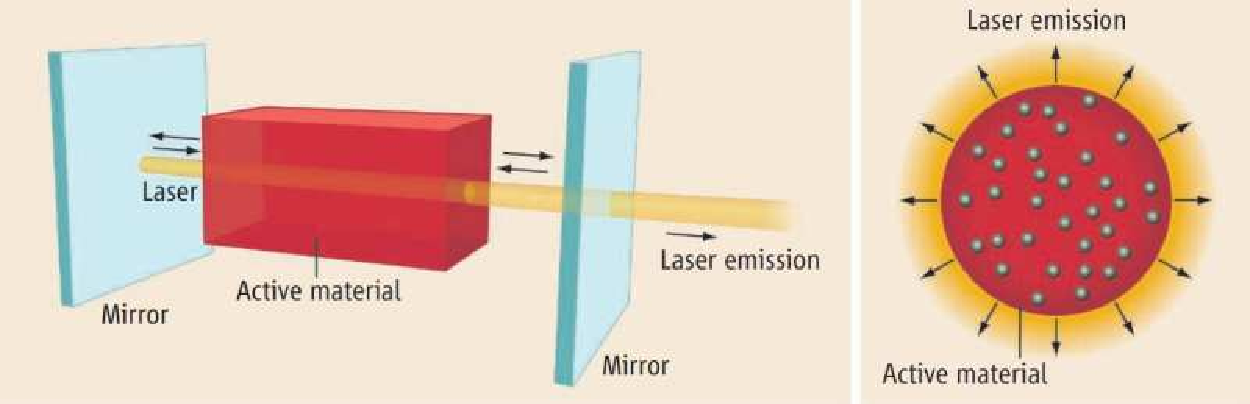
\includegraphics[width=12cm]{./Figs/F1_medium}
\end{center}
\caption[Unified models for light emitting in optical cavities.]{\textbf{Two models for light emitting in optical cavities.} (Left) Sketch of a conventional Fabry-Perot (F-P) laser cavity model: Light is tightly confined by a cavity with a given geometry shape that defines the resonant cavity modes and laser frequency. (Right) A random laser cavity model: Light is scattered by a set of photon emitting particles which modify the optical properties of the optical cavity. This thesis discusses the modification effect of emitters ensemble to the optical cavities in the linear optical regime. From~\cite{Bravo-Abad2008}. Reprinted with permission from AAAS.}
\label{unifiedlasermodel}
\end{figure}



%This work is an extension of previous success on a few excitons coupled cavities studies using scattering model~\cite{Yao2009b,Yao2009c,Yao2009a,VanVlack2011,Reitzenstein2010,Hughes2009,Kristensen2011}. %But for GF calculations involving a large amount of emitters, present works are only limited to a few cases, either within a very narrow frequency range~\cite{Averkiev2009} or ignoring iterated interactions between emitters~\cite{VanVlack2011}, because fully calculation using GF method is a memory- and CPU-time-costly work. This paper will report the spectral modification effects of up-to thousands of emitters for coupled cavities in a broad frequency range and with fully scattering interactions.

%Beyond the motivation in physics mentioned above, there is also a personal motivation strongly driving me to answer some sophisticated questions in the course of researching in theoretical physics. Not too long since I began to study at Queen's University, something really shocking happened to me. Issues arose with my previous supervisor around difference concerning basic principles, which I believe should not be given up. I was thinking about the meaning of life, the driving power of this world, and how I can survive this crisis. The world became both ugly and elegant, cold and warm, bitter and sweet, noisy and melodic, detached and crowded, greedy and generous, selfish and altruistic, impartial and fair... I came to a place of acceptance and decided to finish up the scientific research following my own line of inquiry. Collective interaction in nature may offer insight into the secrets I expect to explore and be significant to this world on many levels. This thinking and reflecting has led to the motivations and problems partially reflected in the scientific side of this thesis.
\section{Background}
In this section, to provide background, we present an overview of optical cavities, photon emitters and present commonly used photonic simulation methods.

\subsection{Optical Cavities}
An optical cavity is a structure that can confine the light in a limited space called cavity, and creates a relatively strong optical field to enhance light-matter interactions. A typical optical cavity is formed by arranging a set of ``mirrors'' or reflecting surfaces in a certain pattern so that the light is reciprocally reflected between them, and the optical fields of different light paths are superimposed to give a strong optical field in the cavity. The most simple pattern of mirror arrangement gives a cavity called Fabry-Perot (F-P) cavity, which has two plane mirrors in parallel to each other (see Fig.~\ref{unifiedlasermodel} left).

The reflectivity of the mirrors, which is defined as the ratio of the power of the reflected light to that of the incident light, determines how many times the light can travel in between the mirrors before decayed leaking out of the cavity. If a cavity is to induce strong interactions between light and the matter in the cavity, the cavity field must be strong enough, compared to the field strength around an electron without the cavity environment. It is necessary to increase the reflectivity of the mirrors in order to enhance the light-matter interactions in the cavity. The highest reflectivity is $100\%$; however, it is unnecessary to make it so high, because we usually need some output from the cavity for other purposes such as lasing. Once the reflectivity is not $100\%$, there is loss or dissipation in a cavity. The ratio of the energy stored to the lost in a cavity is called the Q-factor, denoted by $Q$. Obviously, the higher is the Q, the stronger the cavity field. A typical $Q$ value for a useful optical cavity ranges from several thousands to $10^8$~\cite{Vahala2003}.

The light confined by a cavity has to be essentially a standing wave, otherwise, it will be weakened and canceled by the many superpositions in the cavity~\cite{Novotny2006}. In this sense, an optical cavity is also called an optical resonator. Actually, lasers are typical applications of optical cavities, due to the frequency selection function of cavities. There are certain frequencies that survive, in which the light can permitted to propagate in a cavity. Each frequency corresponds to one mode or more. A mode is defined as a field distribution pattern for a given cavity at a certain frequency. The mode is mainly determined by the geometry of the cavity. The mode volume, $V_{eff}$, describes the concentration of normalized field strength considering the distribution of the refractive index of the cavity medium. It has a unit of volume. If the cavity field is well confined in a small region, the photon emitter in this region can be strongly coupled to the cavity field and show some non-classical or quantum behaviors. The coupling strength, $g\propto 1/\sqrt{V_{eff}}$, describes how strongly a photon emitter is coupled to the cavity field and is forced to emit or absorb photons under the influence of the cavity.  The smaller the mode volume is, the more the cavity field concentrates, and the more clearly the quantum behaviors are observed. To be specific, in this thesis we mainly focus on microcavities, which have typical mode volumes smaller than $10^3\,\mu m^3$. Some microcavities can emit single photon in each emission pulse~\cite{Schwagmann2011,Yao2009a}.

The $Q$ factor can be also defined as the confinement time in units of optical period, such that $Q=\frac{2\pi\tau}{T}=\frac{\omega_c}{\Gamma_c}$, where $\tau$ is the average lifetime of a photon in the cavity, $T$ is the optical period of a given cavity mode, $\omega_c$ is the mode's angular frequency, and $\Gamma_c=1/\tau$ is the decay rate of the cavity. In the presence of cavity decay, the cavity spectrum has a bandwidth, spectral width or linewidth characterized by $\Gamma_c$. The study of this thesis mainly focuses on how the cavity resonance, $\omega_c$, and decay rate or spectral width, $\Gamma_c$, are changed, with the coupling of many photon emitters. By understanding the mechanism of emitter-cavity interactions, one can design and fabricate novel photonic devices for optical communication, quantum computing and many other applications. Before stepping into light-matter interaction, we introduce some typical microcavities.

Microcavities have different structures.  The ones of interest in this thesis are realized in semiconductors which are good materials to form photon emitters included in a cavity. The cleavage planes of semiconductor crystals can be used as the mirrors for a F-P cavity. However, the reflectivity of a cleavage plane is too small to form a high-Q cavity. A distributed Bragg reflector (DBR), which is formed from multiple layers of alternating materials with varying refractive index, is usually used to enhance the Q-factor of a F-P type cavity. A micropillar laser~\cite{Vahala2003} is formed by using DBRs in 1-dimention (1-D). To further increase the Q-factor, 2- and 3-D confinements of light are helpful. A whispering-gallery-type cavity is a 2- or 3-D confined cavity, in which the light is reflected around the circular or spherical wall through total internal reflection.

A photonic crystal (PC) cavity is another type of high dimensional confined cavity. A PC is a photonic structure which has periodic variation of refractive index in 1-D, 2-D or 3-D space. The periodic structure creates a certain frequency band called photonic forbidden band or band gap (PBG), so that a light in this band cannot propagate. By adding a ``defect'' in the PC structure, a permitted narrow band is formed in a certain direction so that a light in this small frequency range is allowed to emit out of the cavity in a certain direction while reflected in the other directions through total internal reflection. The periodic arrangement of refractive index forms the photonic lattice. A ``defect'' in a PC structure is a break region of the periodical structure to form a cavity. It implies that a PC cavity is a photonic structure with periodic variation of refractive index and with a defect. The micropillar laser is a 1-D PC cavity.

The 2-D PC cavity studied in this thesis is called the H3 PC cavity. It is formed from a thin slab of material with a triangular lattice with three neighboring holes (usually airholes) removed in a line to form the cavity (see Fig.~\ref{FDTDsimulation}). A triangular lattice is a pattern of holes arrangement that every three nearest holes are on the vertexes of a equilateral triangle, where the side length of the triangle is the lattice period or pitch. The H3 PC cavity provides a large PBG for TE-like light in the slab made by InP, GaAs or silicon~\cite{Johnson2002a}. With a given material of slab, the resonance of the cavity can be tuned by changing the pitch, the radius of the holes or the distance between the airholes at the ends of the cavity. The uniformity of the hole sizes and positions, the roughness of fabrication, and the distance between the airholes at the ends of the cavity affect the decay rate of the cavity~\cite{Akahane2003}. The silicon-based H3 PC cavity used in this thesis is set to have the following parameters: the lattice period $a=420$ nm, the radius of the holes $r=115.5$ nm, the distance between the holes at the ends of the cavity is $1806$nm, and the thickness of the slab is $210$ nm. The finite difference time domain (FDTD) simulation (will be introduced shortly) gives the resonance of $191.551$ THz, the effective mode volume of $\sim 0.07\,\mu m^3$ and $Q$ is above $45,000$. The refractive index of the slab used in our FDTD simulation is $3.46$. We do not use the Q-factor and the decay rate obtained from FDTD simulation in our exciton-cavity interaction analysis, rather we numerically set the decay rate and Q-factor to match with published studies. According to the relationship of $Q=\frac{\omega_c}{\Gamma_c}$, therefore, the cavity resonance may be different from the FDTD simulation result. In most cases, we set $\Gamma_c=0.1$ meV, which gives $Q\approx 8000$.

\begin{figure}[htp]%[floatfix]
\centering
\begin{center}
%\DeclareGraphicsRule{.pdf}{eps}{}{`convert #1 eps:-}
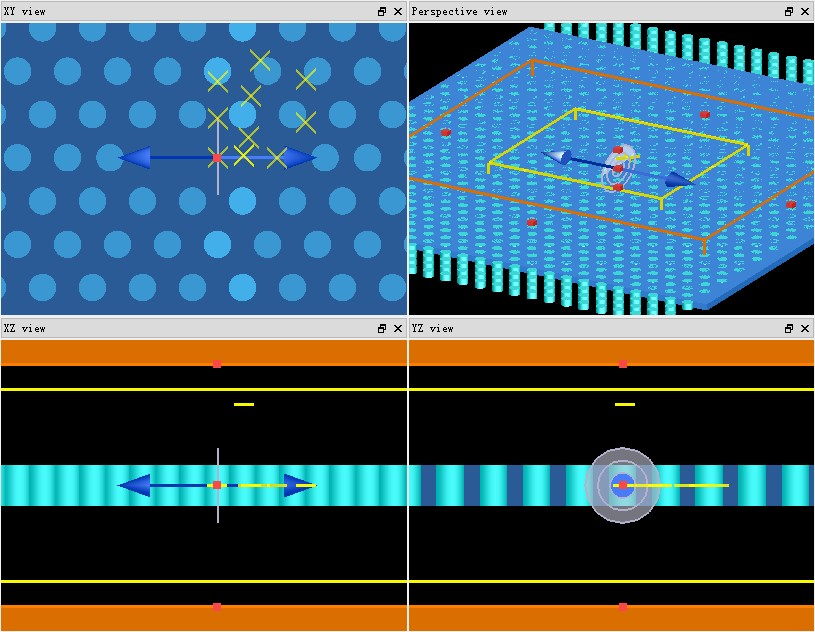
\includegraphics[width=10cm]{./Figs/FDTDsimulation}%[bb=1.0in 1.0in 7.5in 10in]
\end{center}
\caption[An FDTD simulation diagram of a H3 PC cavity.]{\textbf{An FDTD simulation diagram of a H3 PC cavity.} Top right shows the 3-D bird-view of the cavity configuration under simulation. Top left shows the zoomed-in top-view on the cavity, where three airholes (in light blue) are removed from the triangle lattice. Bottom left shows the $x$-$z$ view. Bottom right shows the $y$-$z$ view. Double arrows indicate a dipole source is in the center of the cavity. Cross signs indicate the in-site time monitors in an FDTD simulation.}
\label{FDTDsimulation}
\end{figure}


A PC cavity structure can be fabricated using epitaxial growth technique and standard semiconductor planar processing technology. The slab can be grown layer by layer using metalorganic vapor phase epitaxy (MOCVD) or molecular beam epitaxy (MBE) technologies in the scale of $0.1$ nm or so~\cite{III2009}. The components and growth conditions can be monitored and tuned in real-time to control the growth quality. Quantum wells and quantum dot layers can be formed by tuning growth conditions such as temperature, pressure, flow rate or supplying rate and so on. After the slab is grown, photolithography technology can be used to form the pattern of the hole arrangement. Some type of photoresist and a patterned mask are used in the photolithography process, and the pattern in the mask is transformed to the photoresist layer on top of the slab. Some parts of the photoresist layer are removed under $X$-ray exposure in the process. By using wet etching or dry etching technologies, the pattern is consequently transformed to the arrangement of holes by vertically etching off the materials of the slab uncovered by photoresist.


\subsection{Quantum Dots and Optical Emitters}
A cavity without photon emitters is useless unless the cavity is used as a pure coupler to an incident light. Photon emitters in a cavity can generate absorption and gain so that a laser or a light beam with a certain property is emitted from the cavity, and make the cavity functional. In this thesis, we only consider quantum photon emitters, which emit light mainly through quantum transitions or quantum jumps rather than thermal radiations. Some types of atoms, ions and electron-hole pairs in a certain environment can be the units of such quantum photon emitters, which emit photon through the transition of electrons in them from a high level to a low level, or through annihilation of electron-hole pairs (will be introduced in Chapter~\ref{ch:theory}). A nitrogen vacancy, a quantum well or a quantum dot (QD) provides the necessary environment for quantum transitions. Because of good thermal characteristics and excellent optical and electronic performances, QDs are widely used. We will use QDs as an example of quantum emitters in our discussion.

%Electrical and optical pumps are two ways to excite the emitters. In this thesis, we only interest in optical pump case, in which a pumping light is emitted to the cavity; the emitters absorb the light and re-emit the light with the interaction of the cavity. The emitted light usually has different properties such as frequency and bandwidth from the incident light. The differences and the mechanism is the study topic in this thesis.

In a simple model, a QD can be treated as a 0-D or 3-D quantum box, which confines electrons in a small condensed space. The electrons in a QD have discrete energy levels because of the quantum confinements from the nearby interface atoms. The energy discretization makes the quantum transition of states possible to emit photons. In practice, a QD is usually made of semiconductor materials such as InGaAs/GaAs, AlGaAs/GaAs and Ge/Si. As mentioned earlier, QDs can be grown through epitaxial growth technique~\cite{Schliwa2009}, which grows semiconductor materials layer by layer. Through changing the growth conditions, dot-shape bumps can be formed. Those bumps are quantum dots. We call the QDs grown in this method as self-assembled QDs, which are randomly distributed in a layer. QDs can also be grown through Hydrothermal method and sol-gel growth method, in forms of random nanocrystals. Self-assembled QDs usually have a dimension of $5\sim 150$ nm, a intrinsic decay rate ranging from several to several tens of $\mu$eV, and a density of $10^{10}\sim 10^{11}$/cm$^2$~\cite{Amano2006}. The size of a QD affects its emission resonance or frequency; the quality of growth and the slab environment affect its decay dynamics. Typically, there can be more than thousands of self-assembled QDs in an effective interaction area $\sim \mu m^2$, and the QD resonances are distributed in a Gaussian (normal) distribution profile or a logarithmic normal distribution profile with a standard deviation ranging from several to several tens of meV. We will discuss a cavity with {\textit {discrete}} and {\textit {dense}} QDs in later chapters, where there are several tens and several thousands of quantum emitters respectively.

\subsection{Simulation Methods}
One can simulate the mode distribution and calculate the mode resonance of a cavity using numerical methods. The finite element method (FEM) and finite-different time-domain (FDTD) method~\cite{Taflove2005} are two mature methods for the cavity analysis. The idea is to solve the Maxwell equations of the optical field with boundary conditions determined by the cavity geometry. The FDTD method solves the differential equations in the time domain and through meshing the geometric structure into small unit Yee cells~\cite{Taflove2005}. The FEM solves the corresponding integral form of Maxwell equations with finite Discretization of the cavity geometry structure based on Gauss-Green theorem. Packaged softwares such as PICS3D, COMSOL Multiphysics, R-Soft suit, Lumerical FDTD Solutions and Meep have been developed based on these two methods. We use Lumerical FDTD Solutions~\cite{LumericalSolutions} to simulate the bare cavity properties.

To calculate the cavity mode in FDTD solutions, one has to put a light source into the cavity to generate a propagating optical field in the time domain (see Fig.~\ref{FDTDsimulation}). We use a dipole source as the light source. Note that the dipole sources used in FDTD simulation is not the dipoles studied in this thesis for exciton-cavity interactions. The dipole sources in FDTD simulation can generate a light field as a dot light source under predefined parameters, but it does not interact with the cavity, which means the dipole source's properties cannot be changed by the optical field, and the dipole source cannot scatter light traveling toward it. In fact, there is no mature software which can fully simulate the complex cavity interactions with many photon emitters. This is why we conduct the study present in this thesis.


In our study, at first, we calculate the bare cavity mode without photon emitters using FDTD method; then we include the photon emitters into the cavity system based on Green function (GF) method (will be introduced in the next chapter), in which every photon emitter is treated as a dipole. We will discuss the cases that one- and two-dipole coupled to a cavity, discrete-dipole coupled to a cavity and dense-dipole coupled to a cavity to study the exciton ensemble-cavity or ensemble-cavity interactions in detail. The density of dipole distribution referred in this thesis is mainly used as a concept of describing how close the dipole resonances to each other in the frequency domain rather than in the spatial domain.

\section{Problems}
There are four major questions that I wish to address on the topic of exciton-cavity interactions:

a) How does an ensemble of emitters affect the optical properties of a cavity with which the emitters are coupling?

b) How does a cavity affect an ensemble of individual emitters that are coupling to it? Can we explain the spectral behaviors by considering the collective emitting and light scattering process?

c) Can we always view a photon emitting unit, for example, a QD, as one single exciton? How do optical pumps excite excitons?

d) Upon the excitation of emitters, can the cavity mode and the coupling condition of excitons be changed?


This thesis undertakes to answer these four questions rigorously and scientifically.

%If, for example, one replaces ''emitters'' with ``people'', or replaces ``cavities'' with ''communities''  in the questions above, one may see an aspect of the questions I was concerning myself with the social side. However, in what follows, we will confine our discussion to the interaction of emitters and cavities problems.

Technically, to fully understand the physics of cavity-emitter interaction, we need to calculate every interaction path between cavity and individual emitters. How to calculate the cavity spectrum considering these interaction channels is another problem in our study, which ultimately leads to an open work on making a nanophotonic toolbox to make calculation processing efficient.

\section{Objective}
In this thesis, we calculate the optical parameters of a photonic crystal (PC) H3 cavity (mainly) using the finite-different time-domain (FDTD) method and  calculate the ensemble spectrum of a few QDs in a PC cavity. Then, we develop a method to calculate a dense-emitter-coupling cavity spectrum. Through these calculations and comparing the results with that of simplified models, we answer the four problems referred to above (see Fig.~\ref{Cavity_pump}).

%    \notesbox{Note:  These are the section headings that I decided to use.  Check out several
%    recent theses to decide how you want to lay out your introduction (and conclusion) chapters.}

\begin{figure}[htp]%[floatfix]
\centering
\begin{center}
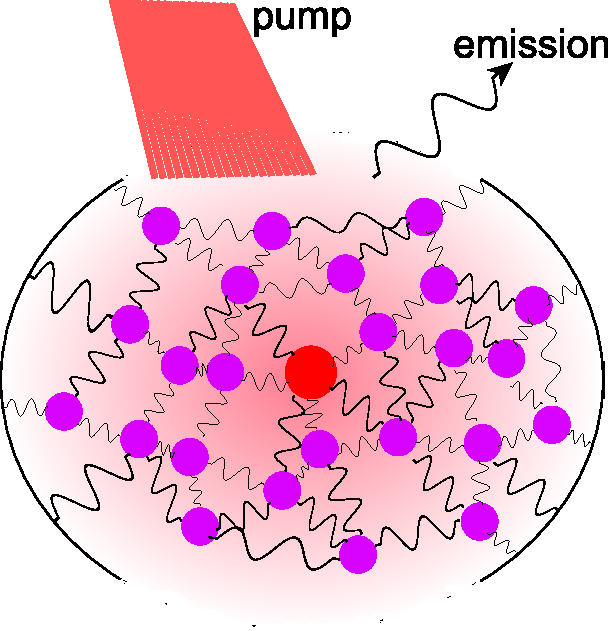
\includegraphics[width=6cm]{./Figs/Cavity_pump}%[bb=1.0in 1.0in 7.5in 10in]
\end{center}
\caption[Many photon emitters are coupled to a cavity.]{\textbf{Many photon emitters are coupled to a cavity.} In the linear optics regime, this thesis will study the changes of the cavity properties, the mechanism of optical pumps and the role of background emitters (purple balls in the figure) to the cavity, a target emitter and their coupling. The red ball at the center of the cavity indicates the target dipole which is on resonance and in a strong field.}
\label{Cavity_pump}
\end{figure}

\section{Hypothesis}
This thesis focuses on the light-matter interaction in a ``general`` schema while also including hypotheses that make our discussion less ``general``. For example, this study always uses the dipole approximation, which means that every exciton excited in photon emitters can be treated as a dipole. Notice that there is no strong correlation between the number of physical emitters, such as QDs, and that of dipoles we are using for our discussion. This assumption is commonly acceptable in the cases in which the electromagnetic field can be viewed as a constant homogeneous field on the scale of an emitter, which is valid for QDs and color centers in normal nanocavities. However, this assumption also means we do not consider the band structure of the emission units; rather, we mainly focus on the emitting and scattering nature of individual emitters merged in a dielectric environment. Hence, our work cannot explain the intraband absorption of QDs, Auger recombination, spin splitting, and other phenomena which involve complex band structures.

For the calculation based on the FDTD method and our Green function (GF) method, we assume that the cavity mode can be described by Maxwell equations, which is usually valid for normal nanophotonic devices, including all the cavity configurations we are going to discuss in this thesis.

For the calculation based on the GF method, we also always use the single excitation approximation~\footnote{There is only one exciton or photon in the cavity.} and only consider the linear effect of dipole-dipole and dipole-cavity interactions, which may not work for high-power pumped cavities or explain the spatial hole burning effect, but is good enough to reveal the physics of ensemble-cavity interaction in our scenarios.




\section{Organization of Thesis}

We begin the thesis by introducing necessary background, including photonic scattering theory and the Green function method, the initial condition of my calculations, as well as the statistical method of master equations in
chapter~\ref{ch:theory}. We discuss typical photonic nanocavities mode calculations with the FDTD method and Green function calculation algorithms, and study the spectrum and GFTs of cavities with a few discrete dipoles in Chapter~\ref{ch:cavity}. The methods and models we used in this thesis will be verified in this chapter. It will also identify the effects of modifying the optical property of a cavity and dipoles. Chapter~\ref{ch:ensemble} describes our work on the spectrum of cavities coupled with a dense quantity of photon emitters using the GF method, compared with master equation (ME) models, for several scenarios of random dipole distributions. Spectral modification effects will be studied in the presence of dense dipoles.
Chapter~\ref{ch:Conclusion} concludes the findings of this study, and outlines the future work. The overall structure of my research is shown in Fig.~\ref{MainStructure}.
Implementation details and long derivations of the calculations, calculation methods and some key formulas are presented in the appendices.

\begin{figure}[htp]%[floatfix]
\centering
\begin{center}
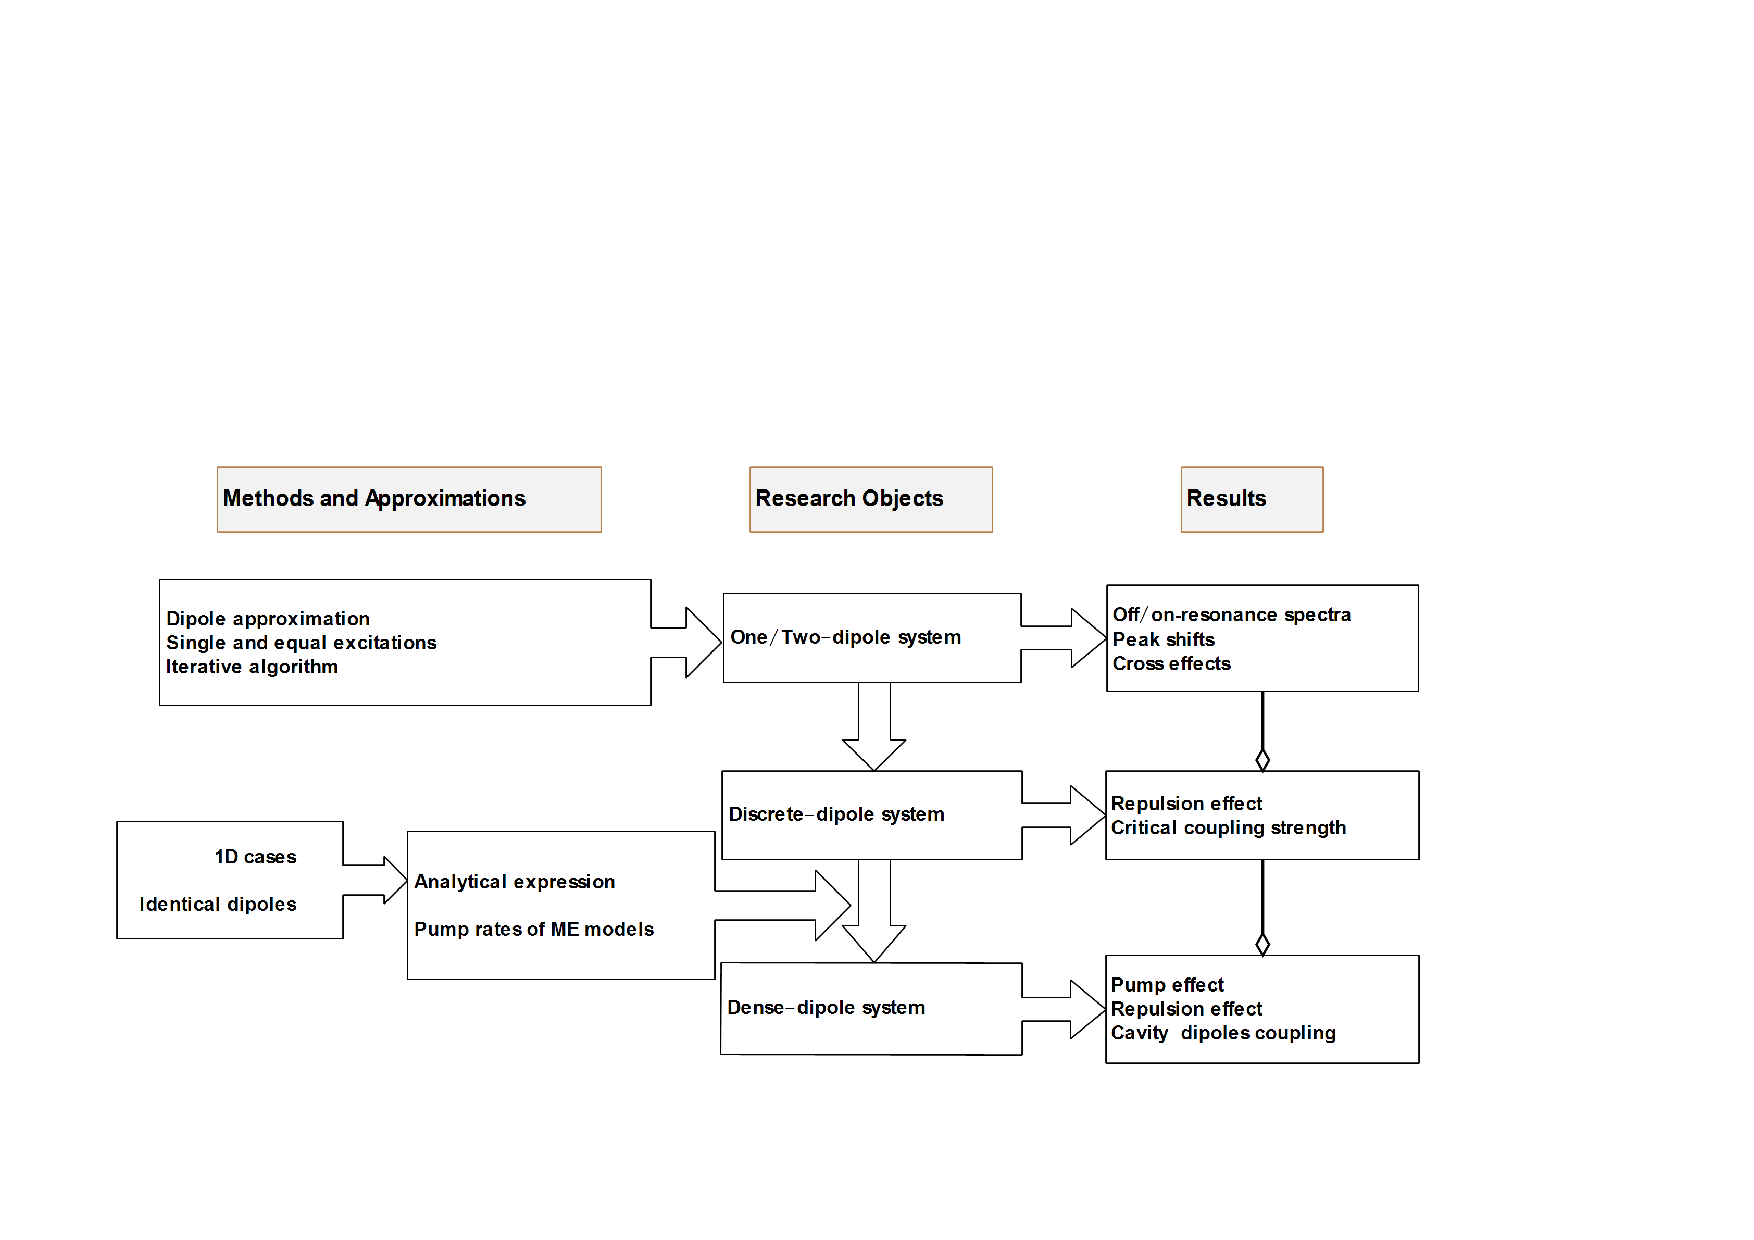
\includegraphics[width=16cm]{./Figs/MainStructure}%[bb=1.0in 1.0in 7.5in 10in]
\end{center}
\caption[Hypotheses, research objects and main results.]{\textbf{Hypotheses, research objects and main results.} }
\label{MainStructure}
\end{figure} 
%\include{Background}
\chapter[Models and Theories]{Models and Theories of Dipoles Coupled to a Cavity}\label{ch:theory}

\section{Dipoles Coupled to a Cavity}
Light has been widely employed to transmit information since the first semiconductor laser was demonstrated by researchers from General Electric and MIT's Lincoln Laboratory in 1962~\cite{Keyes1962}, and an appropriate material for optical fibers was found by Kao and Hockham from International Telephone and Telegraph Company in 1966~\cite{Kao1966}. Light is also believed to be a good candidate for information processing to replace the present electronic processing~\cite{Nagy2006a,Hemmer2005}. A light beam does not interact with another light beam in general, however, which is a big barrier for light control and information processing.

Optical cavities capture light in a confined space and enhance the electromagnetical field through light-reflection and light-scattering, making the control of light easier (see Fig.~\ref{Cavity_withDipoleT}). In a semiconductor, which is the emitter of interest in this thesis, electrons and holes in the conduction band and valence band can controllably annihilate to emit a polarized photon. A bound electron and a hole pair produced by exciting an electron to the conduction band in a semiconductor material is called an exciton. Photon emission by exciton annihilation is generally a dipole quantum transition process. In an inverse process, light can also be absorbed through dipole excitation from a lower energy state to a higher excited state. Here, a dipole is an electronic oscillator which contains a charge oscillating in a electromagnetic field. The dipole approximation is used when the electromagnetic field is approximately constant within the range of electron displacement. In this study, the dipole approximation is always used.

\begin{figure}[htp]%[floatfix]
\centering
\begin{center}
%\DeclareGraphicsRule{.pdf}{eps}{}{`convert #1 eps:-}
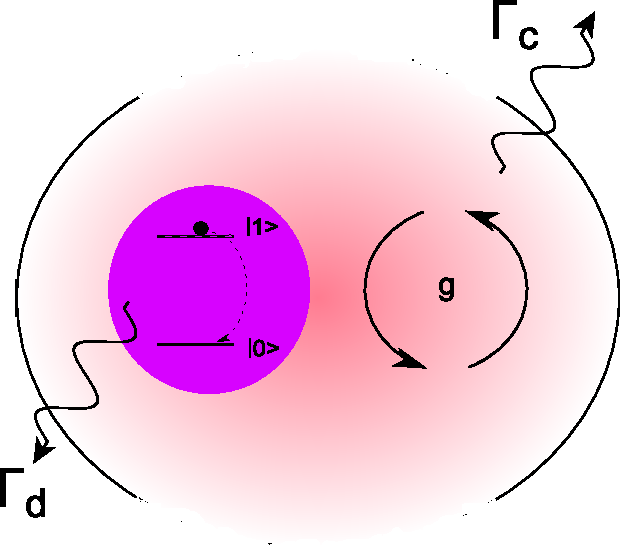
\includegraphics[width=7cm]{./Figs/Cavity_withDipoleT}%[bb=1.0in 1.0in 7.5in 10in]
\end{center}
\caption[A diagram of a cavity with one dipole.]{\textbf{A diagram of a cavity with one dipole.} }
\label{Cavity_withDipoleT}
\end{figure}


In addition to semiconductors, some light-emitting molecules, atoms and ions can also have dipole quantum transitions which emit photons. We also call the excited state of an emitter in those media an exciton, which is the basic unit of light emission~\cite{Gibbs2011}. A quantum dot (QD) is a good example of a photon emitter, in which the electrons are confined in a quantum box and discretely occupy energy levels where quantum transitions can occur under the drive of an external field. Particularly, we will consider the optical pump as a driver of light emission in this thesis.

A dipole can be viewed as a two-level system, which has a ground state of $\ket{0}$ and an excited state of $\ket{1}$. As the electron oscillates, it has a resonant frequency of $\Omega_d=(E_1-E_0)/\hbar$ and an optical moment or dipole moment of ${\bm\mu_d}$, where $E_1$ and $E_0$ are the eigen-energies of the excited and ground states respectively. The optical moment operator for the electron in the Heisenberg representation is defined as
\begin{equation}
\mathbf{\hat{d}}(t)=-e\mathbf{\hat{r}}(t),\label{eq:dt1}
\end{equation}
where $e$ is the unit charge, and $\mathbf{\hat{r}}$ is the position operator for the electron. The position operator determines the spatial distribution of charge and its time evolution. If we assume the dipole is in $\ket{\Psi}=1/\sqrt{2}(\ket{0}+\ket{1})$ at a given time $t=0$, the dipole moment can be measured as ${\bm\mu_d}=-e\bra{0}\mathbf{\hat{r}}\ket{1}$.  Considering a harmonic form of oscillation~\cite{Gerry2005,Mahan2000}, one can rewrite the optical moment operator as
\begin{equation}
\mathbf{\hat{d}}(t)={\bm\mu_d}[\hat{\sigma}_d^-(t=0) e^{-i(\Omega_d-i\Gamma_d/2) t} +\hat{\sigma}_d^+(t=0)e^{i(\Omega_d+i\Gamma_d/2) t}],\label{eq:dt2}
\end{equation}
where $\hat{\sigma}^{+/-}_d$ are Pauli operators for the exciton, and $\Gamma_d$ is the decay rate of dipole oscillation, which can be measured as the full-width-half-maximum (FWHM) of its spectrum. The $\hat{\sigma}^{+}_d$ operator is defined as $\hat{\sigma}^{+}_d=\ket{1}\bra{0}$, which moves a dipole from the ground state $\ket{0}$ to the excited state $\ket{1}$; in contrast, the $\hat{\sigma}^{-}_d$ operator is defined as $\hat{\sigma}^{-}_d=\ket{0}\bra{1}$, which moves a dipole from the excited state $\ket{1}$ to the ground state $\ket{0}$. Writing $\mathbf{\hat{d}}(\omega)=\int_{0}^{+\infty}{dt e^{i\omega t}\mathbf{\hat{d}}(t)}$, one obtains the quantum dipole moment operator in the frequency domain as
\begin{equation}
 \label{dipole}
  \mathbf{\hat{d}}(\omega) =
{i\bm\mu_d}\left [ \frac{\hat{\sigma}_d^-(t=0)}
{\omega-\Omega_d+i\Gamma_d/2}+\frac{\hat{\sigma}_d^+(t=0)}{\omega+\Omega_d+i\Gamma_d/2}\right ].
\end{equation}
%By comparing Equs.\eqref{eq:dt1} and~\eqref{eq:dt2}, one can obtain
%\begin{equation}
%{\bm\mu_d}=-e\bra{0}\mathbf{\hat{r}}\ket{1}.
%\end{equation}

In our study, the dipoles sit in the optical field of a cavity made by a semiconductor or many other media. Since the electrical field dominates the photon-dipole interactions in our case, we are only concerned with the electric field, or E-field. A cavity is usually characterized by its spectrum or power spectrum, which is defined as the Fourier transform of the modulus square of the time-domain field strength. One can identify the resonance of $\omega_c$ and the decay rate of $\Gamma_c$ in a certain mode. A mode is a defined pattern of the electromagnetic field for a cavity. The mode of a cavity is usually believed to be pre-determined by the bare cavity with a given geometric shape, but in this thesis we will show that the parameters (resonance and decay rate, or spectral width) of the cavity can be changed in the presence of photon emitters.

The mode of a bare cavity, where no photon emitters are added, can be calculated using some software, such as Lumerical Solutions~\cite{LumericalSolutions} based on FDTD method, which we used throughout the course of the research in this thesis.

%The interaction between dipoles and cavities can be


As nanophotonic innovation and nanotechnology march on, high-Q (optical quality) cavities can be achieved commonly~\cite{Akahane2003, Akahane2005}, and photon emitters can be implanted in a cavity accurately~\cite{Reithmaier2004, Reitzenstein2008}. As a result, some exciting or unexpected phenomena have been witnessed because of the interaction between a large number of individual emitters and a coupled optical cavity. For example, researchers have observed spectral broadening effects in InAs/InGaAs quantum dots (QDs) in a semiconductor photonic nanocavity~\cite{Tawara2008}. Meanwhile, cavity enhancement and spectral narrowing effect in nitrogen vacancy (NV) center(s), QD(s) and golden nano-particles have also been observed experimentally~\cite{Wolters2010, Faraon2011, Reithmaier2004, Englund2005, lodahl2004controlling}. An in-depth study of cavity-ensemble emission is used to explain these experimental phenomena and to predict new properties.

%\begin{figure}[H]
%\centering
%\begin{center}
%\includegraphics[width=8cm]{./Figs/pc}
%\end{center}
%\caption[Diagram of a Photonic Crystal H3 cavity with QDs.]{\textbf{Diagram of a Photonic Crystal H3 cavity with QDs.}  }
%\label{pc}
%\end{figure}

%\begin{figure}[H]
%\centering
%\begin{center}
%\includegraphics[width=8cm]{./Figs/Pillar_arrows}
%\end{center}
%\caption[Diagram of a micropillar cavity with QDs.]{\textbf{Diagram of a micropillar cavity with QDs.}  }
%\label{pillar}
%\end{figure}

%So far, however, theoretical studies on this topic are largely focused on few emitters coupled cavity luminescence~\cite{Hughes2009, Hughes2007, Xu2000, Averkiev2009}, or studied under truncated parameters by reducing an ensemble of emitters as one single emitter~\cite{Laussy2006, Reboul2009, Schwab2006, Illes2010a}, or studied without sophisticated considering the interaction between emitters~\cite{Meldrum2010}, and so on.

There are many models to explain the collective luminescence in a cavity field, but there are few based on the microscopic scattering process among a large number of emitters and the cavities. Rate equations and master equation (ME) methods are two widely used statistical methods suitable for a huge number of emitters and a few emitters cases~\cite{Hughes2009, Hughes2007, Xu2000, Averkiev2009}, respectively. Some phenomenological parameters, such as pumping rate, come from parameter fitting rather than first principles coefficients. Some of the ME methods only focused on one or two strongly coupled excitons~\cite{Laussy2006, Reboul2009, Schwab2006, Illes2010a}, and truncated the ensemble effect into phenomenological parameters. Other researchers try to adjust ME models to $N$-exciton coupled cavities~\cite{Illes2010a,Laussy2011}, but discussions are limited to a few excitons strongly coupled cavities, and these models can hardly explain the inhomogeneous broadening effect with a large number of background excitons, as we will discuss later. The ME-based Monte Carlo method and quantum trajectory method~\cite{Nowak2008,Meldrum2009,Temnov2005} have the same drawbacks of employing phenomenological parameters, and so far none has explicitly shown the spectral shifting effects.  A model based on Fermi's golden rule was developed by Meldrum to assess the spectral inhomogeneous broadening effect~\cite{Meldrum2010}, but it doesn't consider emitter-emitter interactions and hence may not be able to reflect well the spectral shifting effect. Among these models, moreover, it is still difficult to explain how light travels in the cavity and among the ensemble of photon emitters and hence revises the optical property of the cavity, as the models mainly focus on the energy transmission between levels and individuals, and assume that both the corresponding luminescence frequencies and modes are essentially determined by the bare cavity in which the photon emitters are not added.

As discussed in the introduction, the Green function method may be a good method to calculate ensemble effects in optical cavities. This chapter will introduce some basic features of the GF method and the models we are going to use in the remaining chapters. In the next section, we will first introduce the approach to calculate bare cavity GFs, and then discuss how to effectively calculate the GFs with $N$ dipoles. The initial conditions and the cavity spectrum calculation theory will be discussed next. The ME method will also be introduced at the end of this chapter.

%The initial motivation for the study throughout this thesis is to provide a general theory fully considering the interaction between emitters and cavity in linear region, and explain the detuning effect to cavity optical properties caused by coupled individual emitters, and how a cavity affects the interaction among emitters.

\section{Green Function Method of Optical Emission and Scattering}
This section will be introduced following the diagram in Fig.~\ref{FromG2S}.

\begin{figure}[htp]%[floatfix]
\centering
\begin{center}
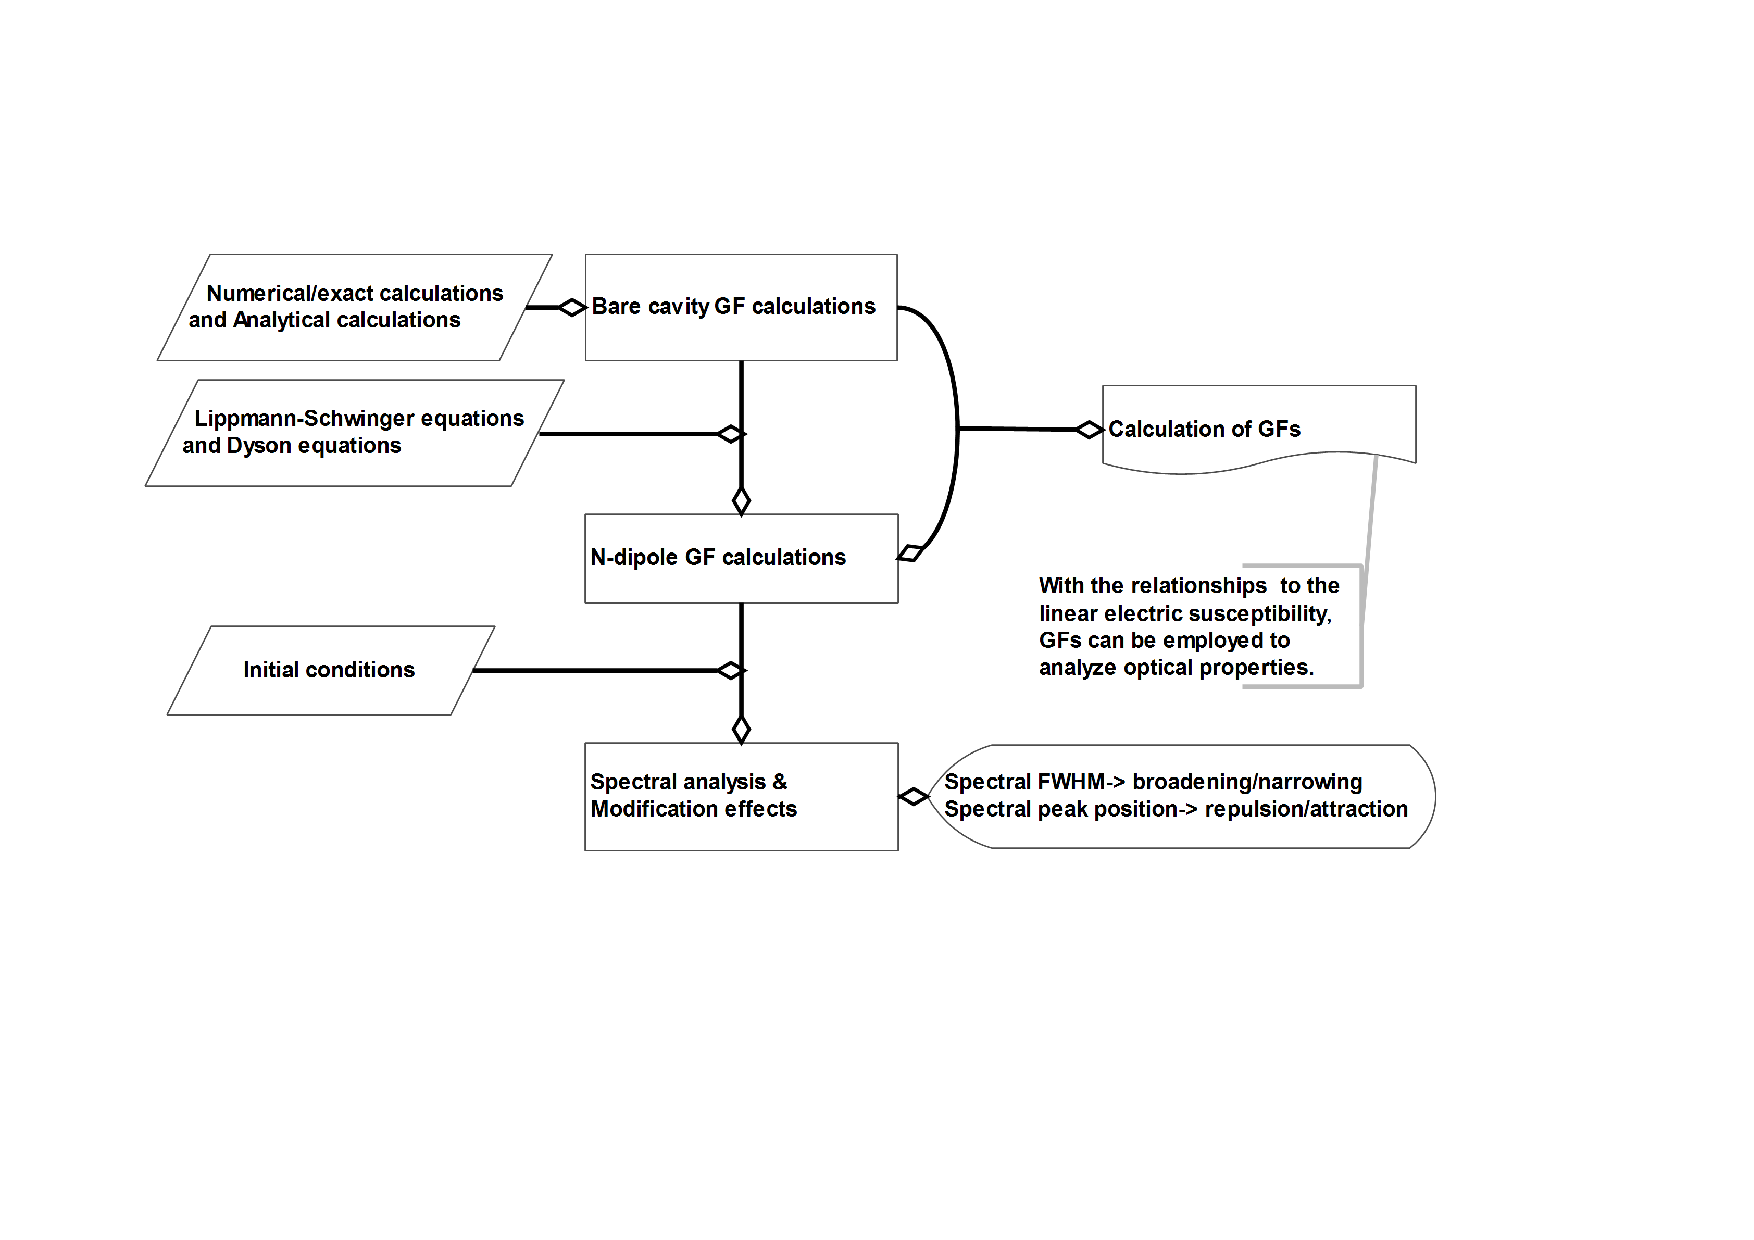
\includegraphics[width=16cm]{./Figs/FromG2S}%[bb=1.0in 1.0in 7.5in 10in]
\end{center}
\caption[The diagram of Green function theory for the exciton-cavity study.]{\textbf{The diagram of GF theory for the exciton-cavity study.} }
\label{FromG2S}
\end{figure}

\subsection{Classical GFT and FDTD method}\label{section:GFT}
In an optical cavity or a waveguide, corresponding to a given mode $\mathbf{f}_\lambda(\mathbf{r})$, the Maxwell equations give~\cite{Wubs2004}
\begin{equation}
 \label{eq:Maxwell}
-\nabla \times \nabla \times \mathbf{f}_\lambda(\mathbf{r}) + \varepsilon(\mathbf{r})(\omega_\lambda/c)^2 \mathbf{f}_\lambda(\mathbf{r}) = 0,
\end{equation}
where we have made $\lambda=(\mathbf{k},s)$, $k=\omega/c$, and $s$ is the polarization degenerate index (determined by the symmetry of the cavity or waveguide). Here, the mode $\mathbf{f}_\lambda(\mathbf{r})$ is
a harmonic solutions of the Maxwell equations for the inhomogeneous dielectric in absence of dipoles. If we put a dipole into the dielectric at ${\bf r}'$, there is a classical Green function tensor (GFT), $\Grrw$, detected at ${\bf r}$. $\varepsilon(\mathbf{r})$ is the permittivity of the medium at ${\bf r}$.
Notice that we limit our discussion of the GFTs to the frequency domain and only the electric GFTs--
the Magnetic GFTs, $\mathbf{G}_M(\rr, \omega)$ can be discussed similarly. The GFT corresponding to mode $\mathbf{f}_\lambda(\mathbf{r})$ is defined by a wave equation similar to Eq. (\ref{eq:Maxwell})
but with a dipole source  (generally a polarized source, described by a delta or Lorentzian function, based on the dipole approximation)
on the right-hand side, which is given by
\begin{equation}
\label{def:GEwave}
 -\nabla \times \nabla \times \mathbf{G}(\rr,\omega) + \varepsilon(\mathbf{r})(\omega/c)^2 \mathbf{G}(\rr,\omega) = \mathbf{I} \delta \left(\br-\br'\right).
\end{equation}
The GFT defined above describes how the wave propagates from source $\mathbf{r}'$ to detector $\mathbf{r}$. The total GFT can be decomposed into transverse and longitudinal parts, $\mathbf{G}^T(\rr,\omega)$ and $\mathbf{G}^L(\rr,\omega)$, respectively. That is,
\begin{equation}
\mathbf{G}(\rr,\omega)=\mathbf{G}^T(\rr,\omega)+\mathbf{G}^L(\rr,\omega),
\end{equation}
where the longitudinal part is given by~\cite{Wubs2004}
\begin{equation}
\label{GL}
\mathbf{G}^L(\rr,\omega)=\frac{\boldsymbol{\delta}_{\varepsilon}^L \left(\br',\br\right)}{\varepsilon(\mathbf{r})(\omega_\lambda/c)^2}.
\end{equation}
The $\boldsymbol{\delta}_{\varepsilon}^L \left(\br',\br\right)$ in the equation above is the generalized longitudinal delta function in a dielectric medium, and is defined as the difference between the ordinary Dirac, $\mathbf{I} \delta \left(\br-\br'\right)$,
and the generalized transverse delta function, $\boldsymbol{\delta}_{\varepsilon}^T \left(\br',\br\right)$. The transverse delta function is defined as
\begin{equation}
\boldsymbol{\delta}_{\varepsilon}^T \left(\br,\br'\right)
=\sum_{\lambda}{\mathbf{f}_\lambda^*(\mathbf{r})\mathbf{f}_\lambda(\mathbf{r}') \varepsilon(\mathbf{r}')},
\end{equation}
and has the projection property $\int{d\br' \boldsymbol{\delta}_{\varepsilon}^T \left(\br',\br\right) \cdot \mathbf{X}^T(\br')}=\mathbf{X}^T(\br)$ for any transverse vector field  $\mathbf{X}^T(\br)$.
In Equ.\eqref{GL}, the generalized longitudinal delta function in a dielectric medium, $\delta_{\varepsilon}^L \left(\br-\br'\right)$, and hence $\mathbf{G}^L(\rr,\omega)$ gives a countable effect only when $\br=\br'$. In most cases in this thesis referring to high-Q cavities, one can approximate the total GFT by the transverse GFT, which means
\begin{equation}
\mathbf{G}(\rr,\omega) \approx \mathbf{G}^T(\rr,\omega),
\end{equation}
which can be a Lorentzian function, as will be discussed in Section~\ref{section:Lorentz} and Appendix~\ref{App:analyticalGF}.

If the background E-field at $\br$ is $\mathbf{E}_0$, then the E-field at $\br$ responding to a polarized source at $\br'$ is given by
\begin{equation}
 \label{EandGwithE0}
\mathbf{E}=\mathbf{E}_0+\mathbf{G} \cdot \mathbf{P},
\end{equation}
where $\mathbf{P}$ is the source's polarization vector or polarization density.
Now, we let $\mathbf{E}_0=0$, which means there is no initial E-field at the detector's position.
Hence, one has
\begin{equation}\label{eq:EGP}
\mathbf{E}=\mathbf{G} \cdot \mathbf{P}.
\end{equation}
In terms of matrices, the equation above can be written as
\begin{align}
\label{EandGwithoutE0}
\left( \begin{array}{c}
       E_x\\
       E_y\\
       E_z  \end{array} \right)
                   = \left( \begin{array}{c}
                      G_{xx} \quad G_{xy} \quad G_{xz} \\
                      G_{yx} \quad G_{yy} \quad G_{yz} \\
                      G_{zx} \quad G_{zy} \quad G_{zz}  \end{array}  \right) \left( \begin{array}{c}
                                                                                     P_x\\
                                                                                     P_y\\
                                                                                     P_z
                                                                                    \end{array} \right).
\end{align}
If we let the polarization source only have $x$ component or orientate the polarized source to $x$ direction, which means
\begin{equation}
 \label{Px}
\mathbf{P}=\left( \begin{array}{c}
                   P_x\\
                   0\\
                   0
                  \end{array} \right),
\end{equation}
then only the first column of GFT contributes to the measured E-field, and from Eq. (\ref{EandGwithoutE0}) we obtain
\begin{equation}
 \label{Gix}
G_{ix} \equiv \frac{E_{i}}{P_x}, \quad (i=x, y, z).
\end{equation}
The $G_{ix}\,(i=x, y, z)$ stretch out the first column of the GFT.
Similarly, if we orientate the polarized source to $y$ and $z$ direction, we can get the second and third column of GFT.
All the discussions above form the basis of the FDTD method to obtain GFT for our configuration.


The FDTD method is a numerical method to calculate the time domain electromagnetic field propagating in an arbitrary optical structure.
Further, we can get frequency domain results by operating a Fourier transformation from the time domain fields,
and get the background Green function tensor components as
\begin{equation}
 \label{def:GFT}
 G_{ij}(\rr,\omega)=\frac{{\rm FT}[E^i_\lambda(\mathbf{r},t)]}{{\rm FT}[E^j_d(\mathbf{r}',t)]}
=\frac{E^i_\lambda(\mathbf{r},\omega)}{E^j_d(\mathbf{r}',\omega)}, \quad (i,j=x, y, z),
\end{equation}
where we assume the test dipole source is located at $\mathbf{r}'$ and only has a $j$ component of polarized electric field $E^j_d(\mathbf{r}')$
(we have replaced $ \mathbf{P}$ with $\mathbf{E}_d$, which is the observed E-field at the source and already includes the dielectric effect),
and the detector is located at $\mathbf{r}$ with $i=x, y, z$ components of electric field $E^i_\lambda(\mathbf{r})$, ${\rm FT}$ indicates Fourier transformation.
When we apply this formula in a waveguide or a cavity, the electric field $\mathbf{E}_\lambda$ here
can be the electric mode $\mathbf{f}_\lambda$ used above.

If $\br=\br'$, the real part of the Green function usually diverges~\cite{Dung2003}. We can use the imaginary part to identify the Green function:
\begin{equation}
 \label{GFTimag}
 {\rm Im}(G_{ij}(\br',\br',\omega))={\rm Im}\left(\frac{{\rm FT}[E^i_\lambda(\mathbf{r}',t)]}{{\rm FT}[E^j_d(\mathbf{r}',t)]}\right)
={\rm Im}\left(\frac{E^i_\lambda(\mathbf{r}',\omega)}{E^j_d(\mathbf{r}',\omega)}\right),
\end{equation}
where ${\it Im}$ means the imaginary part of a quantity.



For a dipole source $\mathbf{r}'=\mathbf{r}_d$ in an FDTD calculation (if using Lumerical Solutions~\cite{LumericalSolutions}), we have
\begin{equation}
 \label{def:dipleft}
E^j_d(\mathbf{r}_n,t)=-\frac{\mu_n^j}{\varepsilon_0}\exp(-2\ln(2)\frac{(t-t_0)^2}{\tau^2})\cdot\sin[\omega_0(t-t_0)],\quad j=x, y, z,
\end{equation}
where $\mu_n^j$ is the $j$th component of the dipole moment in a Cartesian coordinate, $t_0$ is the time delay of the dipole source,
and $\tau$ is the FWHM of the dipole pulse. Equ.~\eqref{def:dipleft} shows that the dipole oscillates at mode $\omega_0$ with a Gaussian amplitude profile in the time domain. So, through Fourier transformation, we can get
\begin{equation}
 \label{dipolefw}
E^j_d(\mathbf{r}_n,\omega)={\rm FT}[E^j_d(\mathbf{r}_n,t)].
\end{equation}

In practice, one can run an FDTD calculation in Lumerical, for example, and follow the steps listed in Appendix \ref{App:FDTD_GFT} to calculate the background or bare cavity GFTs.

Note that, in the linear optics of dielectric material, we have~\cite{Boyd2003}
\begin{equation}
\mathbf{P}=\varepsilon_0\mathbf{\chi} \cdot \mathbf{E},
\end{equation}
or
\begin{equation}\label{eq:polarization}
\mathbf{E}=\frac{1}{\varepsilon_0}\mathbf{\chi}^{-1} \cdot \mathbf{P},
\end{equation}
where $\mathbf{\chi}$ is the electric susceptibility of the medium.
By comparing Equ.\eqref{eq:EGP} with the linear polarization equation above, one can find that Equ.\eqref{eq:EGP} is identical to the linear optical polarization equation by defining
\begin{equation}
\mathbf{G}\equiv \frac{1}{\varepsilon_0}\mathbf{\chi}^{-1}.
\end{equation}
This relationship above shows that the GF method we use in this thesis corresponds to a linear optics model for a given optical structure. Moreover, once we obtain the GFs, we equivalently know the $\mathbf{\chi}$. Since $\mathbf{\chi}$ determines the optical properties such as dispersion, absorption, resonant shift and spectral broadening~\cite{Boyd2003,Cohen-Tannoudji1998,Haug1990,Maier2007,Novotny2006,Gerry2005,Sakoda2005}, we can analyze the optical properties of a given optical structure through calculating the GFs. In this study, we focus on the spectral behavior including resonant shift and spectral broadening effects of optical cavities with many dipoles.

%%%%
\subsection{Quantum Description of an Optical Cavity with $N$ Dipoles}
%In the scale of an atom, interactions should be described by full quantum operators in principle.
In a lossless cavity, to describe quantized light emission in an arbitrary inhomogeneous dielectric with relative dielectric function $\varepsilon(\mathbf{r})$ and a finite number N of embedded
dipoles in it, we employ a canonical Hamiltonian in the absence of dephasing and decoherence \cite{Vats2002,Wubs2004}:
\begin{equation}
\label{eq:h}
\begin{split}
 \hat{H} =& \hat{H}_{X}+\hat{H}_F+\hat{H}_I\\
=& \sum_n\hbar \Omega_n \hat{\sigma}_n^+\hat{\sigma}_n^-+
\sum_\lambda\hbar \omega_\lambda
\hat{a}_\lambda^\dagger\hat{a}_\lambda +\sum_{n,\lambda}(
\hat{\sigma}_n^- + \hat{\sigma}_n^+)(g_{n\lambda}
\hat{a}_\lambda+g_{n\lambda}^*\hat{a}_\lambda^\dagger),\\
\end{split}
\end{equation}
where the dipole is at the spatial position $\mathbf{r}_n$; $\hat{a}_{\lambda}^{\dagger}$ and $\hat{a}_{\lambda}$ represent the field mode operators to give the field Hamiltonian $\hat{H}_F=\sum_\lambda\hbar \omega_\lambda
\hat{a}_\lambda^\dagger\hat{a}_\lambda$; $\hat{\sigma}^{+/-}_n$ are the Pauli operators of the excitons
(for excitons that are in the frequency regime of interest) to give the exciton Hamiltonian $\hat{H}_{X}=\sum_n\hbar \Omega_n \hat{\sigma}_n^+\hat{\sigma}_n^-$;
the remaining exciton-photon interaction terms are treated within the dipole approximation
($\hat{H}_I=-\sum_n{\bm{\mu} _n \cdot \hat{\mathbf{E}}(\mathbf{r}_n)}$ corresponding to $\delta$-form polarization
\begin{equation}\label{eq:P}
\hat{\mathbf{P}}_n(\mathbf{r},t)=\delta(\mathbf{r}-\mathbf{r}_n)\bm{\mu} _n(\hat{\sigma}_n^- + \hat{\sigma}_n^+),
\end{equation}
valid for photon emitters whose spatial size is much smaller than a wavelength); we have assumed that there is no decay for individual dipole oscillation. The time dependence is implicit in the Heisenberg picture, and all derivations are under the approximation of single excitation.
In addition, $\Omega_n$ is the resonant frequency of the $n$th exciton, and $\omega_\lambda$ is the eigenfrequency
corresponding to the bare cavity modes of the system ($\mathbf{f}_\lambda(\mathbf{r})$) excluding the dipoles. The coupling strength between the dipole at $\br_n$ and the cavity mode field is given by~\cite{Wubs2004}
\begin{equation}
g_{n\lambda}=-i\sqrt{\frac{\hbar\omega_\lambda}{2 \varepsilon_0}}\boldsymbol{\mu}_n\cdot \mathbf{f}_\lambda(\mathbf{r}_n).
\end{equation}

The Heisenberg equations of motion for the operators can be derived from  $\dot {\hat O}_i = -i{\hbar^{-1}[\hat O_i,H]}$,
yielding~\cite{Wubs2004}
\begin{align}
\frac{d\hat{a}_\lambda}{dt}&=-i\omega_\lambda \hat{a}_\lambda-i\sum_n\hbar^{-1}g_{n\lambda}^*(\hat{\sigma}_n^-+\hat{\sigma}_n^+), \label{eq:a-t}\\
%
\frac{d\hat{a}_\lambda^\dagger}{dt}&=i\omega_\lambda \hat{a}_\lambda^\dagger+i\sum_n\hbar^{-1}g_{n\lambda}(\hat{\sigma}_n^-+\hat{\sigma}_n^+), \label{eq:a+t}\\
%
\frac{d\hat{\sigma}_n^-}{dt}&=-i\Omega_n\hat{\sigma}^-_n-i\hbar^{-1}\sum_{\lambda}(g_{n\lambda}
\hat{a}_\lambda+g_{n\lambda}^*\hat{a}_\lambda^\dagger), \label{eq:sig-t} \\
%
\frac{d\hat{\sigma}_n^+}{dt}&=i\Omega_n\hat{\sigma}^+_n+i\hbar^{-1}\sum_{\lambda}(g_{n\lambda}
\hat{a}_\lambda+g_{n\lambda}^*\hat{a}_\lambda^\dagger). \label{eq:sig+t}
%
%\frac{d\hat{\sigma}_{nz}}{dt}&=2i\hbar^{-1}\sum_{\lambda}(\hat{\sigma}_n^-- %\hat{\sigma}_n^+)(g_{n\lambda}
%\hat{a}_\lambda+g_{n\lambda}^*\hat{a}_\lambda^\dagger).
\end{align}

Next we perform a Laplace transform to positive frequency space,
$O(\omega)=\int_0^\infty dt e^{i\omega t}\, O(t)$, and obtain \cite{Wubs2004}:
\begin{align}
{\hat{a}_\lambda(\omega)}&= \hat{a}_\lambda(t=0) + \frac{i\hbar^{-1}}{\omega-\omega_\lambda}
\sum_n g_{n\lambda}^*[\frac{\hat{\sigma}_n^-(t=0)}{\omega-\omega_\lambda}
+\frac{\hat{\sigma}_n^+(t=0)}{\omega+\omega_\lambda}]\nonumber\\
& \quad + \frac{\hbar^{-2}}{\omega-\omega_\lambda}
\sum_{n,\lambda'} \frac{2g_{n\lambda}^*\Omega_n}{\omega^2-\Omega_n^2} [g_{n\lambda'}
\hat{a}_{\lambda'}(\omega)+g_{n\lambda'}^*\hat{a}_{\lambda'}^\dagger(\omega)], \label{eq:aw} \\
{\hat{a}_\lambda^\dagger(\omega)}&=\adag_\lambda(t=0) - \frac{i\hbar^{-1}}{\omega-\omega_\lambda}
\sum_n g_{n\lambda}^*[\frac{\hat{\sigma}_n^-(t=0)}{\omega-\omega_\lambda}
-\frac{\hat{\sigma}_n^+(t=0)}{\omega+\omega_\lambda}]\nonumber\\
& \quad + \frac{\hbar^{-2}}{\omega+\omega_\lambda}
\sum_{n,\lambda'} \frac{2g_{n\lambda}\Omega_n}{\omega^2-\Omega_n^2} [g_{n\lambda'}
\hat{a}_{\lambda'}(\omega)+g_{n\lambda'}^*\hat{a}_{\lambda'}^\dagger(\omega)],
\label{eq:adaggerw} \\
\hat{\sigma}_n^-(\omega)&=\frac{i\hat{\sigma}_n^-(t=0)}
{\omega-\Omega_n}+\frac{\hbar^{-1}}{\omega-\Omega_n}
\sum_{\lambda}[g_{n\lambda}
\hat{a}_\lambda(\omega)+g_{n\lambda}^*\hat{a}_\lambda^\dagger(\omega)], \label{eq:sig-w} \\
\hat{\sigma}_n^+(\omega)&=\frac{i\hat{\sigma}_n^+(t=0)}
{\omega+\Omega_n}-\frac{\hbar^{-1}}{\omega+\Omega_n} \sum_{\lambda}[g_{n\lambda}
\hat{a}_\lambda(\omega)+g_{n\lambda}^*\hat{a}_\lambda^\dagger(\omega)]. \label{eq:sig+w}
%\hat{\sigma}_{nz}(\omega)&=\frac{i\hat{\sigma}_{nz}(t=0)}
%{\omega}+\frac{2\hbar^{-1}\mu_n\hat{E}_\mu(\mathbf{r}_n)\ast
%[\hat{\sigma}_{n}^-(\omega)-\hat{\sigma}_{n}^+(\omega)]}{\omega}.
\end{align}
%
Here,
\begin{equation}
 \label{eq:Esum}
 \mathbf{\hat{E}}(\mathbf{r},t)=\mathbf{\hat{E}}^+(\mathbf{r},t)+\mathbf{\hat{E}}^-(\mathbf{r},t)=i\sum_\lambda\sqrt{\frac{\hbar
\omega_\lambda}{2\varepsilon_0}}\hat{a}_\lambda(t)\mathbf{f}_\lambda(\mathbf{r})+h.c.
\end{equation}
where the mode expansion of the inhomogeneous field operator $\mathbf{\hat{E}}$
has a sum of a positive-frequency part $\mathbf{\hat{E}}^+$ (containing only annihilation operators in the time domain or positive frequency components in the frequency domain through Fourier transformation)
and its Hermitian conjugate $\mathbf{\hat{E}}^-$, where
\begin{equation}
 \label{eq:E^plus}
 \mathbf{\hat{E}}^+(\mathbf{r},t)=i\sum_\lambda\sqrt{\frac{\hbar\omega_\lambda}{2\varepsilon_0}}\hat{a}_\lambda(t)\mathbf{f}_\lambda(\mathbf{r}).
\end{equation}
Notice that $\mathbf{\hat{E}}(\mathbf{r},t)$ here is equal to a non-interacting (no dipoles embedded) electric field operator everywhere, except at the positions $\mathbf{r}_n$ of the dipoles,
since the dipoles couple to fields in which their own polarization fields are included.
When we use $\mathbf{\hat{E}}(\mathbf{r}_n,t)$ at the dipole position $\mathbf{r}_n$,
it means a self-interaction polarization is included in the dipole self-coupling field; otherwise such a distinction is not necessary.


Using  Equ.\eqref{eq:aw} and~\eqref{eq:adaggerw}, and the expansion of $\mathbf{\hat{E}}$ (Equ.\eqref{eq:Esum}),
we obtain the electric field operator \cite{Wubs2004}:
%
\begin{subequations}
\label{eq:ew1_1}
\begin{align}
\mathbf{\hat{E}}(\mathbf{r},\omega) =& \mathbf{\hat{E}}^{(0)}(\mathbf{r},\omega)\label{bareE0_1}\\
&+ \sum_n{\mathbf{K}(\mathbf{r},\mathbf{r}_n,\omega)\cdot\hat{\mathbf{S}}_n(\omega)}\label{sourceE_1}\\
&+ \sum_n{\mathbf{K}(\mathbf{r},\mathbf{r}_n,\omega)\cdot\mathbf{U}_n(\omega)\cdot\mathbf{\hat{E}}(\mathbf{r}_n,\omega)}\label{scatteringE_1}
\end{align}
\end{subequations}
%
\begin{equation}
 =\mathbf{\hat{E}}^{(0)}(\mathbf{r},\omega)+ \mathbf{\hat{E}}_{source}(\mathbf{r},\omega)+\mathbf{\hat{E}}_{scatt}(\mathbf{r},\omega)\label{eq:E0sourcescatt_1},
% This is an important equation.
\end{equation}
where $\mathbf{K}(\mathbf{r},\mathbf{r}',\omega)$ is the Green function in the context of quantum description, $\hat{\mathbf{S}}_n(\omega)$ is the source operator, and $\mathbf{U}_n(\omega)$ is the scattering potential. The $\mathbf{K}(\mathbf{r},\mathbf{r}',\omega)$ can be defined as a dyadic quantity or a tensor by
\begin{equation}
 \label{K}
 \mathbf{K}(\mathbf{r},\mathbf{r}',\omega)=c^2\sum_\lambda\frac{\mathbf{f}_\lambda(\mathbf{r})\mathbf{f}_\lambda^*(\mathbf{r}')}
{(\omega^2-\omega_\lambda^2)}\frac{\omega_\lambda^2}{\omega^2},
\end{equation}
where we have assumed that the dipole moments are real and  we
have exploited the fact that the summation over $\lambda$ includes
contributions from $\mathbf{f}_\lambda$ and $\mathbf{f}_\lambda^*$ (per $\lambda$)
in the sum.
%(both are solutions
%of an equivalent eigenvalue problem).

Equ.\eqref{eq:ew1_1} is an exact Lippmann-Schwinger equation, and it describes the scattering of and emission by dipoles inside an inhomogeneous dielectric, both for strong and weak dipole-field interactions\footnote{The strong coupling occurs when the dipole-field coupling strength (which is half the Rabi frequency), is faster than any underlying dissipative rate and larger than $1/\tau$ where $\tau$ is the interaction time~\cite{Kimble1998}.}.
More clearly, we can represent the Lippmann-Schwinger equation as three parts (as shown in Equ.\eqref{eq:E0sourcescatt_1}): an undisturbed term
(first term), a source term (second term), and a scattering term (third term).


For the first term, Equ.\eqref{bareE0_1}, the operator $\mathbf{\hat{E}}^{(0)}(\mathbf{r},\omega)$ is the electric field in the absence of the dipoles, with both the positive and negative frequency parts and only depends on input light.


The term (\ref{sourceE_1}), corresponding to $\mathbf{\hat{E}}_{source}(\mathbf{r},\omega)$ in (\ref{eq:E0sourcescatt_1}) account for the field radiated by the dipoles. It is a sum of every dipole with a product of Green function tensor and an emitting source operator $\hat{\mathbf{S}}_n(\omega)$,
which is a vector and has the form $\mathbf{e}_n\hat{S}_n(\omega)$ in the direction of the atomic or exciton's dipole moment \cite{Wubs2004}, and
\begin{equation}
 \label{source}
 \hat{S}_n(\omega) \equiv \left(\frac{i\mu_n\omega^2}{\varepsilon_0c^2}\right)
\lbrack\frac{\hat{\sigma}_n^-(t=0)}{\omega-\Omega_n}+\frac{\hat{\sigma}_n^+(t=0)}{\omega+\Omega_n}\rbrack
=\frac{\omega^2}{\varepsilon_0c^2}\hat{d}_n(\omega),
\end{equation}
where we have plugged in Equ.\eqref{dipole} with $\Gamma_n=0$.
Since both Equ.\eqref{source} and Equ.\eqref{dipole} only depend on $\hat{\sigma}^{+/-}_n$, the Pauli operators of the excitons,
we can see that the second term includes the dipoles and its function is to describe emitting sources.
The initial expectation value of this term can be obtained if we know the initial states and the $n$th dipole's optical momentum \(\boldsymbol{\mu}_n\).

The term (\ref{scatteringE_1}), corresponding to $\mathbf{\hat{E}}_{scatt}(\mathbf{r},\omega)$ in (\ref{eq:E0sourcescatt_1}), contains two parts in every element of the summation for every dipole:
the optical potentials $\mathbf{U}_n(\omega)$ produced at the on-site dipole
and the initial electric operator $\mathbf{\hat{E}}(\mathbf{r}_n,\omega)$ measured at the corresponding dipole position $\mathbf{r}_n$.
$\mathbf{U}_n(\omega)$ is a dyadic and
\begin{equation}
 \label{Udyadic}
\mathbf{U}_n(\omega)=\mathbf{e}_nU_n(\omega)\mathbf{e}_n,
\end{equation}
 where
\begin{equation}
 \label{Un}
 U_n(\omega) \equiv \left(\frac{\mu_n^2\omega^2}{\hbar\varepsilon_0c^2}\right)
\left(\frac{2\Omega_n}{\Omega_n^2-\omega^2}\right),
\end{equation}
and
\begin{subequations}\label{directproduct}
\begin{align}
\mathbf{e}_n\mathbf{e}_n=& \mathbf{e}_n \otimes \mathbf{e}_n\\
=& \left( \! \begin{array}{cc}
    e_n^x \\ e_n^y \\ e_n^z
   \end{array} \! \right)
\left(\, e_n^x\quad e_n^y \quad e_n^z \, \right)=\left( \! \begin{array}{c}
                                  e_n^xe_n^x\quad  e_n^xe_n^y\quad  e_n^xe_n^z\\
                                  e_n^ye_n^x\quad  e_n^ye_n^y\quad  e_n^ye_n^z \\
                                  e_n^ze_n^x\quad  e_n^ze_n^y\quad e_n^ze_n^z
                                 \end{array} \! \right)
\end{align}
\end{subequations}
is the tensor direct product.
Correspondingly, if we omit the factor $(\frac{\omega^2}{c^2})$, we can have the polarization
\begin{equation}
 \label{alpha}
 \alpha_n(\omega) \equiv \frac{\mu_n^2}{\hbar\varepsilon_0}\,\frac{2\Omega_n}{\Omega_n^2-\omega^2},
\end{equation}
which is directly connected to the dipole polarization tensor or dyadic
${\bm \alpha}_n(\omega) = {\bf e}_n \alpha_n(\omega){\bf e}_n$. Whether you prefer to use $\mathbf{U}_n(\omega)$ or ${\bm \alpha}_n(\omega)$,
this part of the term strongly depends on the resonant frequencies $\pm\Omega_n$ and will become sharp and change sign when $\omega$ goes through the dipole resonances.
The electric field operator can set to be the initial background (cavity) electric field operator, with the form as shown in Equ. (\ref{eq:Esum}).
The initial expectation value of this operator can be calculated
according to the given initial dressed states (actually, the cavity's or photons' parts) and normalized modes $\mathbf{f}_\lambda$ at $\mathbf{r}_n$.
Considering all these effects, in terms of physics, we call it the scattering term.


Now, $\Krrw$ is a quantum Green function tensor defined from a fully quantized Lippmann-Schwinger equation~\cite{Wubs2004}.
According to Wubs's work~\cite{Wubs2004}, there are simple relationships among the quantum Green function tensor, $\Krrw$, the classical transverse Green function tensor, $\GTrrw$, and the classical total Green function, $\Grrw$, which we discussed in the last section:
\begin{equation}
 \label{KG}
 \Krrw=\Grrw+\frac{\mathbf{I}\delta(\mathbf{r}-\mathbf{r}')}{\varepsilon(\mathbf{r})(\omega/c)^2}
=\GTrrw+\frac{\bm{\delta}^T(\rr)}{\varepsilon(\mathbf{r})(\omega/c)^2},
\end{equation}
where $\mathbf{I}$ is the unit dyadic, and $\bm{\delta}^T(\rr)
=\sum_\lambda{\mathbf{f}_{\lambda}(\mathbf{r})\mathbf{f}_{\lambda}^*(\mathbf{r}')}\varepsilon(\mathbf{r})$
is a generalized transverse delta function. Notice that the factor $(\omega/c)^2$ is ignored in some publications (for example, see Ref.~\cite{Yao2009a,Hughes2007}).

According to this relationship,  the dyadic $\Krrw$ differs from the total Green function tensor of the medium and its transverse component only when its two position arguments $\mathbf{r}$ and $\mathbf{r}'$ coincide.
%Although different from $\mathbf{G}$, the quantity $\mathbf{K}$ will also be called a Green function.
Because of this, we can make $\mathbf{K}=\mathbf{G}$ in most situations without any problem,
and through calculating the classical Green function to equivalently obtain $\mathbf{K}$.


If $\mathbf{r}=\mathbf{r}'$, all Green functions usually become divergent in their real parts.
Especially when $\mathbf{r}=\mathbf{r}_n$, the self-interaction inevitably makes the Green function divergent.
For these reasons, at $\mathbf{r}=\mathbf{r}'$ we use only the (finite) imaginary part of the background Green tensor, assuming that the effect of the (divergent) real part is already contained in the measured electron mass and transition frequency. Likewise, we will not explicitly include local field effects \cite{Martin1994} in the model but assume that
the effects are included in the measured dipole moments and transition frequencies of the emitters.

In a nutshell, we can resort to the classical Green function to get the quantum Green function just by identifying them
to be equal and using the imaginary part if divergent.

One simple way to verify the calculation accuracy is to examine the numerical result of GFT in a homogeneous case, where the analytical expression of the imaginary part of GFT can be obtained for both quantum and classical limit (see Appendix~\ref{App:homogeneous}). In the homogeneous case, the local optical density, Purcell factor, Lamb shift and decay rate can be expressed analytically as well.

%To realize this calculation, we may need to employ classical Green Function Tensor (GFT) and FDTD method as described below.



\subsection{Lorentz approximation}\label{section:Lorentz}
In practice, a cavity has optical loss in the forms of radiative and non-radiative decays, which can broaden the cavity mode linewidths, and add in radiative mode contribution to the cavity modes. Technically, one can obtain the exact bare cavity GFTs based on numerical calculations of a cavity field. To obtain an accurate result, however, one has to perform a hard computation task. For example, in the case of a typical H3 silicon PC cavity, which we will demonstrate later, one has to calculate about 12 hours with 12G memory on a Dell XPS 8500 workstation (8-core Intel i7 processors) just with 40 time-domain point monitors or a 2D slice monitor on about $1200\times1200$ nm$^2$ meshing grids with a computational step of $20$ nm. If we want to calculate it at hundreds or more positions, it will be a huge computation task.

Fortunately, as we have tested, a Lorentz approximation to the GFT is good enough for optical cavities with well defined modes~\footnote{The optical cavity modes can be quasi-modes, or primarily dominant modes with resonances $\omega_{c\lambda}$. This format of modes is referring to transverse modes.  See Refs.~\cite{VanVlack2012,Kristensen2011} for details.}. Moreover, as examined using Three-layer GF codes developed by our colleagues, if the center-to-center distance between emitting centers such as QDs is more than 20 nanometers, the evanescent contribution of GFT is negligible. That is to say, one can have the analytical GFT given by
\begin{equation}
 \label{Ganal}
\mathbf{G}^{A}=\mathbf{G}^{A}_{cav}+\mathbf{G}^{A}_{rad}\approx \mathbf{G}^{A}_{cav},
\end{equation}
\begin{equation}
 \label{Gcav}
\mathbf{G}^{A}_{cav}(\br,\br',\omega)=\sum_{c\lambda}{\frac{\omega^2\mathbf{f}_{c\lambda}(\mathbf{r},\omega_{c\lambda})\mathbf{f}_{c\lambda}^*(\mathbf{r}',\omega_{c\lambda})}
{\omega_{c\lambda}^2-\omega^2-i\omega\Gamma_{c\lambda}}},
\end{equation}
where $\mathbf{G}^{A}_{rad}$ is the radiative GFT, which usually does not have an explicit analytical expression; $c\lambda$ denote the modes of the cavity, $\Gamma_{c\lambda}$ is the decay rate~\footnote{Generally, to include decay or loss (characterized by $\Gamma_n$), we can simply add a phenomenological decay constant to the resonance energies of the lossless formulas, i.e.
$\omega \pm \Omega_n \rightarrow \omega\pm \Omega_n +
i\Gamma_n/2$, and $\omega^2- \Omega_n^2+
i\omega\Gamma_n$.\label{fn:decayrevision}} or FWHM of cavity mode $\mathbf{f}_{c\lambda}(\omega)$. We have labeled this form of bare cavity GFT with a superscription, ``A'', meaning ``analytical''.

As can be seen in the equations above, the GFT of a cavity is written in the Lorentz form, which has the same form of function as a dipole oscillation. We call this analytical expression Lorentz approximation.

One advantage of using this analytical expression for bare cavity GFTs is that, now, one only needs to calculate the field distribution in a plane or a volume, for example, using a 2D or 3D mode monitor on the given volume with a relatively easy FDTD computation. This is relatively easy to achieve compared with the usual exact numerical calculation method introduced in Appendix~\ref{App:FDTD_GFT}. The discussions later in this thesis are mainly based on this conclusion we have tested here.

The detailed examination between this analytical expression and numerical calculation of GFTs can be found in Appendix~\ref{App:analyticalGF}.




%\subsection{Contribution from $G^{rad}$}
%As calculated in a three-layer Green function method, the radiative part of Green function $G^{rad}$ is ignitible. ...

\subsection{Green Function Calculation of an Optical Cavity with $N$ Dipoles}\label{section:GN}
So far, we have shown that the background GFTs, in which no photon emitters or dipoles are present, can be approximated as a Lorentzian function; and the $\mathbf{K}(\br,\br',\omega)$ approximates to $\mathbf{G}(\br,\br',\omega)$. Now, we are ready to discuss how to calculate the GFTs including the emitting and scattering effects of $N$ dipoles.

Similar to Equ.\eqref{eq:ew1_1}, the E-field operator including the field term, the source term and the scattering term can be represented in terms of $\hat{\mathbf{E}}^{(N)}(\mathbf{r}_n,\omega)$~\cite{Wubs2004,Kristensen2011}:
\begin{align}
 \Erw &=\E0+\frac{1}{\varepsilon_0}\sum_{n=1}^N{\mathbf{G}^{(0)}(\rrn,\omega)\cdot \dnw} \nonumber \\
 &\quad +\sum_{n=1}^N{\mathbf{G}^{(0)}(\rrn,\omega)\cdot \Alphanw \cdot \hat{\mathbf{E}}^{(N)}(\mathbf{r}_n,\omega)}, \label{E4GNS}
\end{align}
where the quantum dipole moment operator for the dipole at $\br_n$ is $\mathbf{\hat{d}}_n(\omega)$
with the optical moment $\boldsymbol{\mu}_n$, the Pauli operators $\hat{\sigma}^{+/-}_n$ \footnote{In most cases of our calculations, we can safely ignore the creation Pauli operator $\hat{\sigma}^{+}_n$ terms, as they only give vanishing residual\cite{Kristensen}.} and resonance of the $n$th exciton pair $\Omega_n$,
and ${\bm \alpha}_n(\omega) = {\bf e}_n \alpha_n(\omega){\bf e}_n={\bf e}_n \otimes {\bf e}_n \alpha_n(\omega)$ with the definition of $\alphanw$ as
\begin{equation}
\label{alphanw}
\alpha_n(\omega)=\frac{\mu_n^2}{\hbar\varepsilon_0}\,\frac{2\Omega_n}{\Omega_n^2-\omega^2-i\omega\Gamma^{\rm
nr}_n},
\end{equation}
where $\Gamma_n$ is the decay rate of the $n$th dipole. Note that, in Equ.\eqref{E4GNS}, we have used $\dnw$ and $\alphanw$ instead of $\Snw$ and $\Unw$ as has be used in Wubs' work. This selection of variables is consistent with Yao's work (see Refs.~\cite{Yao2009a,Yao2009b} and~\cite{Yao2009c}).

In most cases of our discussion, we let the initial E-field at detector position be zero, which suggests $\E0=0$ and hence
\begin{align}
 \label{E4GNS_0}
 \Erw &=\frac{1}{\varepsilon_0}\sum_{n=1}^N{\mathbf{G}^{(0)}(\rrn,\omega)\cdot \dnw} \\
 &\quad +\sum_{n=1}^N{\mathbf{G}^{(0)}(\rrn,\omega)\cdot \Alphanw \cdot \hat{\mathbf{E}}^{(N)}(\mathbf{r}_n,\omega)}.
\end{align}
The initial condition $\E0=0$ is widely valid when there is no photon emitted to the detector's position, which is usually outside of a cavity.

The implicit scattering type formulation of Equ.\eqref{E4GNS_0} suggests that one can rewrite it in an explicit form as
\begin{equation}
 \label{E4GNS_1}
\Erw =\frac{1}{\varepsilon_0}\sum_{n=1}^N{\mathbf{G}^{(N)}(\rrn,\omega)\cdot \dnw},
\end{equation}
where $\GN(\rr,\omega)$ contains the scattering properties
of all $N$-dipole in the sample, and formally is the self-consistent solution to the Dyson equation~\cite{Martin1998} in the form
\begin{equation}
 \label{dysonGN}
\GN(\rr,\omega)=\mathbf{G}^0(\rr,\omega)+\sum_{n=1}^N{\mathbf{G}^0(\rrn,\omega)\cdot \Alphanw \cdot \GN(\mathbf{r}_n,\mathbf{r}',\omega)}.
\end{equation}

Note that Equ.\eqref{E4GNS_1} is identical to the linear polarization equation (Equ.\eqref{eq:polarization}) by defining the $ij$-th entry of tensor $\chi^{-1}$ as
\begin{equation}
(\mathbf{\chi}^{-1})_{ij}=\frac{\varepsilon_0 \braket{\Erw}_i}{P_j}=\frac{\braket{\sum_n{\mathbf{G}^{(N)}(\rrn,\omega)\cdot \dnw}}_i}{P_j},\quad i,j=x,y,z,
\end{equation}
where the polarization density
$\mathbf{P}=\braket{\sum_n{\dnw}}/V$, $V$ is the medium volume, $P_j$ is the $j$th component of $\mathbf{P}$, and $\braket{\hat{O}} _i$ is the $i$th component of the expectation value of an arbitrary vector operator $\hat{O}$. Therefore, the $\GN$ defines the effective susceptibility of the cavity medium, and determines the optical properties of the cavity. In other words, the light emitting and scattering effects among dipoles in the cavity determines the optical properties of the cavity. Consequently, one can control the cavity properties through adding proper coupled excitons into the cavity.


Now, we discuss how to calculate the GFTs. Considering $r'=r_i,\, i=1,2,3,\cdots,N$ labeling for $N$ dipoles, such that for any given detected position $r$, $\GN(\rr,\omega)$ is only dependent on the interacting GFTs between any two dipoles, namely $\GN(\mathbf{r}_i,\mathbf{r}_j,\omega)$. So, if we can obtain the interacting GFTs among all source pairs, we can easily get the GFTs at any detected positions since we know the background or bare cavity GFTs. Now, let us solve $\GN(\mathbf{r}_i,\mathbf{r}_j,\omega)$, which can be derived from Equ.\eqref{dysonGN} as
\begin{equation}
 \GN(\mathbf{r}_i,\mathbf{r}_j,\omega)=\mathbf{G}^0(\mathbf{r}_i,\mathbf{r}_j,\omega) +\sum_{n=1}^N{\mathbf{G}^0(\mathbf{r}_i,\mathbf{r}_n,\omega)\cdot \Alphanw \cdot \GN(\mathbf{r}_n,\mathbf{r}_j,\omega)}.
\end{equation}


\begin{figure}[htp]%[floatfix]
\centering
\begin{center}
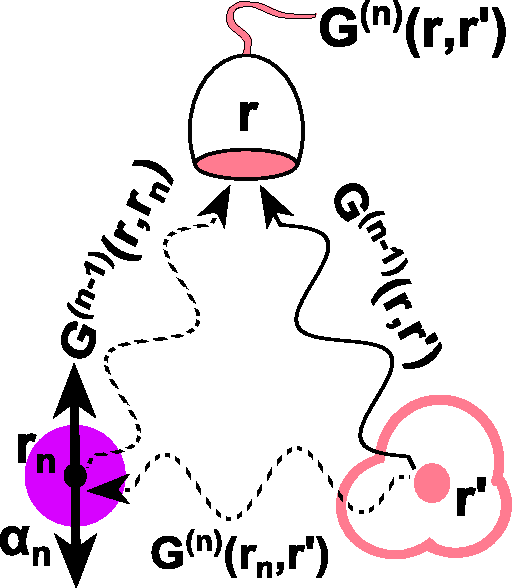
\includegraphics[width=5cm]{./Figs/GnDetection}%[bb=1.0in 1.0in 7.5in 10in]
\end{center}
\caption[The physics picture of Dyson equations.]{\textbf{The physics picture of the $n$-th order Dyson equations for $\Gn(\rr)$.} The solid wave illustrates the direct source emission path from $\br'$ to $\br$. The dashed wave illustrates the scattering path through the $n$-th dipole at $\br_n$. The cloud around $\br'$ illustrates that $(n-1)$ dipoles have been re-normalized as a single unit through the iteration of the $(n-1)$-th order of Dyson equations. }
\label{GnDetection}
\end{figure}

Instead of solving Equ.\eqref{dysonGN} directly, we can also adopt an iterative
scheme by rewriting a series of Dyson equations as
\begin{equation}
 \label{dysonGn}
\Gn(\rr)=\Gm1(\rr)+{\Gm1(\rrn)\cdot {\bm \alpha}_n \cdot \Gn(\mathbf{r}_n,\mathbf{r}')}.
\end{equation}
for $1 \leq  n \leq  N$. Equ. (\ref{dysonGn}) together with the symmetry relation
\begin{equation}
\label{symG2}
 G_{ji} \left(\br',\br,\omega\right) = G_{ij} \left(\br,\br',\omega\right)
\end{equation}
 forms the basis of GFTs and our calculation scheme in which QDs are
added to the system one by one in a self-consistent manner (see Fig.~\ref{GnDetection} for the physics picture). To solve this series of equations, as above, we also first place the detector at dipole positions. It gives interacting terms
\begin{equation}
\label{dysonGnij}
\Gn(\mathbf{r}_i,\mathbf{r}_j)=\Gm1(\mathbf{r}_i,\mathbf{r}_j)+{\Gm1(\mathbf{r}_i,\mathbf{r}_n)\cdot {\bm \alpha}_n\cdot \Gn(\mathbf{r}_n,\mathbf{r}_j)}.
\end{equation}
These interacting GFTs are first worked out for $\mathbf{r}_i=\mathbf{r}_n$, and this result is used to compute GFTs for $\mathbf{r}_i \neq \mathbf{r}_n$. As we increasing $n$ from 1 to $N$, we can solve the full Dyson equations in a straightforward iteration procedure based on bare cavity GFTs, which are supposed to be in Lorentzian forms as
\begin{equation}
 \label{Gcav}
\mathbf{G}^{(0)}(\br,\br',\omega)=\sum_{c}{\frac{\omega^2\mathbf{f}_{c}(\mathbf{r},\omega_{c})\mathbf{f}_{c}^*(\mathbf{r}',\omega_{c})}
{\omega_{c}^2-\omega^2-i\omega\Gamma_{c}}},
\end{equation}
with $c$ denoting modes of the cavity (we consider single mode case as default), $\omega_c$ the mode resonance, $\Gamma_{c}$ the decay rate or FWHM of $\mathbf{f}_{c}(\omega)$ for the corresponding mode.
For simplicity, all formulas below implicitly include the parameter $\omega$ unless explicitly stated otherwise.

Now, let's only consider 1-D case, which means all vectors and tensors are reduced to scalars. This truncation of dimensions is useful to study the optical properties of the cavity-QED system in one polarized direction. We particularly focus on the two simple scenarios, of which the GFs can be solved analytically without using a time-consuming iterative computation procedure.

\subsection{Two Analytical Scenarios}\label{section:scenarios}
In the following two sections, we will start to look at the spectrum of many photon emitters coupled with a single cavity mode, which has a relatively high Q or small non-radiative decay rate, $\Gamma_c$, and a well-defined intrinsic resonance, $\omega_0$. Notice that we define the observed cavity resonance at the peak position of the cavity spectrum as $\omega_c$, which gives $\omega_c \equiv \omega_0$ if there is no exciton coupled to the cavity. We regard every exciton as a dipole. The number of dipoles in a cavity system may not be the number of physical particles, such as QDs, since every particle can be excited to generate zero or many excitons~\footnote{Although excitons with the same resonance are forbidden to be at the same position by the exclusion principle, there can be several excitons with different resonances in a single quantum dot due to multi excited energy levels. One example of more than one exciton in a single elongated quantum dot was studied in Refs.~\cite{Muller2004,Gammon1996}. The existence of many excitons in the case of elongated QDs above is the consequence of shape anisotropy of the QDs.}. We suppose the background dipoles have the same amplitude of optical moments, $\bm{\mu}_n$, yet have different resonances of $\Omega_n$, where the subscript $n$ labels different background dipoles. In most of our discussions, we only look at the spectrum projected in one direction, and all vectors and tensors are reduced to scalars. The resonances of the background dipoles are randomly distributed according to the energy bands of the material, temperature~\cite{Li2005a,Wei2006}, sizes and shapes\cite{Imamoglu1999,Wang2007,Ratchford2011} of QDs, for example. Here, we used a Gaussian distributed dipole ensemble, which has a central resonance of $\Omega_d$ and a standard deviation of $\sigma$.

Below, we will mainly discuss two scenarios for the background dipoles. One is that all dipoles are located in a homogeneous field, with a unique coupling strength, $g_b=g_n=g$, defined by
\begin{equation}
g_{n}=\sqrt{\frac{\omega_c}{2\hbar \varepsilon_0}}\boldsymbol{\mu}_n\cdot \mathbf{f}_c(\mathbf{r}_n),
\end{equation}
where $\mathbf{f}_c(\mathbf{r}_n)=\mathbf{f}_c(\mathbf{r}_n,\omega_c)$ denotes the cavity mode or field strength at the $n$-th background dipole positioned at $\mathbf{r}_n$. In this case, we have assumed that the dot product of dipole moments and the on-site field is constant, and the amplitude of the field strength on the dipole oscillation direction is constant. This scenario is suitable for some micropillar, microdisk and similar devices, which have a smooth and near-homogeneous field strength for the emitting mode.

The other scenario is that there are a few primary or target emitting dipoles strongly excited with relatively large coupling strengths, $g_t$, and all the background dipoles share the same smaller coupling strength, $g_b=g$. To simplify the analysis, we will consider the case with only one target dipole. This scenario is usually suitable for photonic crystal cavities and similar cases which have one or several designed strong field spots to position target emitters. The target dipole will be labeled with subscript $t$.

To calculate the PL spectrum, the method developed by Wubs, Hughes and collaborators~\cite{Wubs2004,Kristensen2011,Wubs2012} was followed, which has been applied to one- and two-QDs coupled micropillar cavity and PC cavity systems\cite{Yao2009b,Yao2009c,Yao2009a,VanVlack2011,Reitzenstein2010,Hughes2009,Kristensen2011}. The key step to calculate the spectrum is to obtain the GFs including $N$ dipoles. Generally, the Green functions can be iteratively solved to obtain numerical values based on Dyson equations presented in the last sections~\cite{Wubs2004}, and cannot be written explicit analytical expressions. It is time- and memory-consuming to numerically calculate the GFs including a large number of dipoles. Fortunately, in the two scenarios we introduced above, one can obtain the analytical expressions of the Green function with any number of dipoles and complete the statistical analysis of collective emitting effects easily.

We present the main results of the Green functions for the two scenarios introduced above as follows. A detailed derivation can be found in the appendix~\ref{App:GF_ensemble}.

For scenario one, which does not have an identified target dipole, the Green functions including $n$-dipoles (labeled by $(n)$ in the superscripts) are
\begin{align}
\label{Gn11}
 G^{(n)}_{R_b,R_b}&=\frac{G^{(0)}_{R_b,R_b}}{1-G^{(0)}_{R_b,R_b}\sum_i^n{\alpha_i}},\\
\label{GnR1}
 G^{(n)}_{R,R_b}&=\frac{G^{(0)}_{R,R_b}}{1-G^{(0)}_{R_b,R_b}\sum_j^n{\alpha_j}}.
\end{align}
For short hand, we have labeled the first subscript of GFs as the detector,
and labeled the second subscript of GFs as the source.
That is to say, the subscripts of GFs defined in this section correspond to the arguments of detector and source positions in the normal GF definitions. For example, $G^{(n)}_{R,R_b}=G^{(n)}(R,R_b,\omega)$. Again, $\omega$ is implicit for all variables.

%Please notice that both equations ~\ref{Gn11} and ~\ref{GnR1} only have one cumulative variable, which is $\sum_j^n{\alpha_j}$, so to calculate the series of \{$G^{(n)}$\} that we can simply apply high-efficient matrix operators within a few steps by avoiding time-consuming iteration procedure in Matlab.



For scenario two, where there is one target dipole with a relatively large coupling strength and all the other background dipoles are in a mean weak field, the Green functions are
\begin{subequations}
\label{G1RR}
\begin{align}
 G^{(1)}_{R_t,R_j} &=\frac{G^{(0)}_{R_t,R_j}}{1-G^{(0)}_{R_t,R_t}\alpha_t},\quad j=t,b,\\
  G^{(1)}_{R,R_t} &=\frac{G^{(0)}_{R,R_t}}{1-G^{(0)}_{R_t,R_t}\alpha_t}, \\
  G^{(1)}_{R,R_b} &=G^{(0)}_{R,R_b}+\frac{G^{(0)}_{R,R_t}\alpha_t G^{(0)}_{R_t,R_b}}{1-G^{(0)}_{R_t,R_t}\alpha_t},\\
  G^{(1)}_{R_b,R_b} &=G^{(0)}_{R_b,R_b}+\frac{G^{(0)}_{R_b,R_t}\alpha_t G^{(0)}_{R_t,R_b}}{1-G^{(0)}_{R_t,R_t}\alpha_t},\label{G1RbRb}
\end{align}
\end{subequations}
and for $n\geq 1$
\begin{subequations}
\label{Gn+1RtRj}
\begin{align}
 G^{(n+1)}_{R_t,R_j} &=\frac{G^{(n)}_{R_t,R_j}}{1-G^{(n)}_{R_t,R_t}\alpha_t} \label{Gn+1RtRj1}\\
&= \frac{G^{(1)}_{R_t,R_j}}{1-G^{(1)}_{R_b,R_b}\sum_p^n{\alpha_p}},\quad j=b,t,\label{Gn+1RtRjexpand}
\end{align}
\end{subequations}
\begin{align}
  G^{(n+1)}_{R,R_b} &=\frac{G^{(1)}_{R,R_b}}{1-G^{(1)}_{R_b,R_b}\sum_i^n{\alpha_i}},\\
 G^{(n+1)}_{R,R_t} &=G^{(n)}_{R,R_t}+\frac{G^{(n)}_{R,R_b}\alpha_n G^{(n)}_{R_b,R_t}}{1-G^{(n)}_{R_b,R_b}\alpha_n}, \label{Gn+1RRt}\\
  G^{(n+1)}_{R_b,R_b} &=\frac{G^{(1)}_{R_b,R_b}}{1-G^{(1)}_{R_b,R_b}\sum_i^n{\alpha_i}}.\label{Gn+1RbRb}
\end{align}

Again, the equations above indicate that the Green functions including $N$ dipoles depend on the coupling term of all background dipoles. The difference between the two scenarios is that the target dipole changes the bare Green functions and hence the Green function including the target dipole plays a role as the bare Green functions do in scenario one. We would also like to keep Equs.\eqref{Gn+1RtRj1} and~\eqref{Gn+1RRt} in the iterative forms, which indicate the scattering effect from the $n$ background dipoles to the target dipole.

Also notice that the GFs of scenario one and scenario two are similar to one- and two-dipole coupled cavities, if comparing them with the formulas in, for example, Refs.~\onlinecite{Yao2009c,Kristensen2011}. The only difference is that the self energy term~\cite{Mahan2000}, $\sum_j^n{\alpha_j}$, replaces an individual $\alpha$, which is used for few-dipole cases. Therefore, the sum term indicates that the coupled background dipoles oscillate as an entity. Particularly, if all background dipoles share the same resonance and optical moment, it leads to
\begin{equation}
\sum_j^n{\alpha_j}=n\alpha,
\end{equation}
which means that, if we treat the ensemble as a single dipole, the effective optical moment and effective coupling strength are enlarged by $\sqrt{N}$ folds from the individual dipole. In this case, the GFs are simplified to
\begin{equation}
\label{equivGn11}
 G^{(n)}_{R_b,R_b}=\frac{G^{(0)}_{R_b,R_b}}{1-nG^{(0)}_{R_b,R_b}\alpha},
\end{equation}
\begin{equation}
\label{equivGnR1}
 G^{(n)}_{R,R_b}=\frac{G^{(0)}_{R,R_b}}{1-nG^{(0)}_{R_b,R_b}\alpha}.
\end{equation}

In general, $\alpha$ is a Lorentzian function of $\omega$; however, $\sum_j^n{\alpha_j}$ for an ensemble of dipoles may not be so. This fact leads to inhomogeneous broadening phenomena, as will be discussed in Chapter~\ref{ch:ensemble}. Moreover, scenario one is just a special case of scenario two when $g_t=g_b$.

Because of the clear physical picture and wide applicability, in Chapter~\ref{ch:ensemble}, we will mainly focus on the two scenarios mentioned above. The conclusions should be extendable to more general cases.

%{\textbf{Extension to Coupled-bin Model:}}
%Particularly, if we further make all excited resonant frequencies of QDs as the same value, which gives $\alpha_i=\alpha$, Equs.\eqref{Gn11} and ~\ref{GnR1} can be simplified into
%\begin{equation}
%\label{equivGn11}
% G^{(n)}_{R_b,R_b}=\frac{G^{(0)}_{R_b,R_b}}{1-nG^{(0)}_{R_b,R_b}\alpha},
%\end{equation}
%\begin{equation}
%\label{equivGnR1}
% G^{(n)}_{R,R_b}=\frac{G^{(0)}_{R,R_b}}{1-nG^{(0)}_{R_b,R_b}\alpha}.
%\end{equation}
%compared with first order Green's function and Equ.\eqref{alphanw}, we find that this ensemble is equivalent to one single QD with $\sqrt{n}$ times larger optical moment than real individual QD. And for general cases, ensemble properties cannot be generalized as easy as this particular case. However, if there are $N$ dots around one fixed frequency, their accumulated contribution to the total spectrum is not necessarily be their sum, and spectral amplitudes between two different frequencies also cannot be simply weighted by the corresponding numbers at those frequencies. Strictly speaking, this conclusion is contrast to reference \cite{meldrum2010} where the authors used homogeneous assumption. (More conclusions can be provided, if you are interested in.)

%In reality, researchers usually treat emitters with nearby resonances as one single dipole, or in most cases they can not distinguish individual excitons with close resonance. Equs.\eqref{equivGn11, equivGnR1} provide a theoretical origin of the equivalence between single dipole and many dipoles. Let's call it {\textit{coupled-bin}} model. However, as the cavity plays a role in the interaction, we should not use coupled-bin model or treat one QD as a single dipole any more in some cases. We will discuss it in the end of Chapter~\ref{ch:ensemble}.

\subsection{Incoherent Spectrum of an Ensemble Coupled Cavity}
One goal of calculating GFTs or GFs is to calculate the emission spectrum or field distribution in the presence of $N$ dipoles.
By definition, the emission power spectrum is given by
\begin{equation}
 \label{spectrumdef}
\begin{split}
S(\mathbf{r},\omega) =& \int_0^\infty \!\! \int_0^\infty\!\!
\mathrm{d}t_1\mathrm{d}t_2 \, e^{i\omega(t_2-t_1)}\mathinner{\langle}\hat{\mathbf{E}}^-(t_1)\hat{\mathbf{E}}^+(t_2)\mathinner{\rangle} \\
=& \mathinner{\langle} \left( \int_0^\infty \!\! \mathrm{d}t \, e^{i \omega t} \hat{\mathbf{E}}^+(t) \right)^{\dagger} \, \int_0^\infty \! \!
\mathrm{d}t \, e^{i\omega t} \hat{\mathbf{E}}^+(t) \mathinner{\rangle},
\end{split}
\end{equation}
where
\begin{equation}
 \label{eq:E^plus}
 \mathbf{\hat{E}}^+(\mathbf{r},t)
 =i\sum_\lambda\sqrt{\frac{\hbar\omega_\lambda}{2\varepsilon_0}}a_\lambda(t)\mathbf{f}_\lambda(\mathbf{r}).
\end{equation}
$a_\lambda$ is the annihilation operator for photons with angular frequency of $\omega_\lambda$.
Now,
\begin{align}
\int_0^\infty \! \mathrm{d} t \, e^{i\omega t} \hat{\mathbf{E}}^+(t) &= \int_0^\infty \! \mathrm{d}t \, e^{i\omega t}
\left[ \frac{1}{2\pi} \int_0^\infty \mathrm{d}\omega' \, e^{-i\omega' t} \mathbf{\hat{E}}(\omega')\right]  \nonumber\\
&= \frac{1}{2 \pi} \int_0^\infty \!\! \mathrm{d}\omega' \, \mathbf{\hat{E}}(\omega') \int_0^\infty \!\! \mathrm{d}t \, e^{i(\omega-\omega') t} \nonumber\\
&= \frac{1}{2\pi} \int_0^\infty \! \mathrm{d}\omega' \, \mathbf{E}(\omega')\left[iP(\frac{1}{\omega-\omega'})+\pi\delta(\omega-\omega')\right] \label{specP} \\
&= \frac{1}{2\pi}\pi(\mathbf{\hat{E}}(\omega)+\mathbf{\hat{E}}(\omega))\nonumber\\
&= \mathbf{\hat{E}}(\omega),
\end{align}
where $ P $ is the principle value function~\cite{Carmichael2007}, and Cauchy's integral formula\footnote{See Ref.~\cite{VanVlack2012} for details.} has been used to give $P[1/(\omega-\omega')]=-i\pi$.
The power spectrum can be simply expressed (see also \cite{Hughes2009})
\begin{equation}\label{eq:spectrum}
 S({\bf r},\omega)=\langle
(\mathbf{\hat{E}}(\omega))^{\dagger}\mathbf{\hat{E}}(\omega)\rangle.
\end{equation}
Notice that this is a non-Markovian solution, valid for any spatial position $\mathbf{r}$.

Once the power spectrum or photoluminescence (PL) spectrum is obtained in the frequency domain, it is easy to get the luminescence dynamic curve in the time domain,
merely by performing a Fourier transformation.

From Equ.\eqref{E4GNS_1}, we can get the incoherent spectrum formula for the $N$-dipole coupled cavity system as
\begin{equation}
 \label{spectrum}
 \mathbf{S}(\br,\omega)=\left|\mathbf{E}^{(N)}(\br,\omega)\right|^2,
\end{equation}
where
\begin{equation}
 \left| \mathbf{E}^{(N)}(\br,\omega)\right| =\frac{1}{\varepsilon_0}\langle \sum_n{\GN(\rrn,\omega)\cdot \dnw}\rangle.
\end{equation}

We will discuss the spectra of several cases under the single excitation approximation in the following subsections. At the end of this section,
we will define a proper initial condition for the $N$-dipole coupled cavity,
to be discussed in the next chapters.
%In equations above, subscription ``c'' means cavity term which includes the bare cavity field and scattering term; the subscription ``s'' means source term, which is the contribution from all photon emitters.

Below, we will discuss the initial conditions and spectrum calculations for several cases. As will be shown, to analyze the spectrum of optical cavities with $N$ dipoles, the roadmap that we first calculate the total GFTs including any $n\,(n\leq N)$ dipoles and then calculate the corresponding spectra is feasible and efficient for spectral analysis; the mixed state with equally excited dipoles under the single excitation condition is a good initial condition for our calculation, both because of its simplicity and its representativeness for practical cases. At the end of this section, we will obtain the general spectral formula for the $N$ dipoles coupled cavity under the mixed state initial condition.
\subsubsection{Case 1: One-dipole system initially with one exciton and no photon}

We assume an initially excited dipole at ${\bf r}'={\bf r}_1$,
so that we can write the initial
condition as
$\ket {\Psi(t=0)}=\ket{0}_{\rm c}\ket 1_{\rm x}=\sigp\ket{0}$, where the ket with subscript $x$ indicates whether the dipole is excited, and the ket with subscript $c$ indicates the photon number in the cavity. The ket $\ket{0}$ is the ground state of $\ket{0}_c\ket{0}_x$.

For a one-dipole system, Equ.\eqref{E4GNS} gives the exact electric field operator responding at $\br$ as
\begin{equation}
\mathbf{\hat{E}}^{(1)}(\mathbf{r},\omega)=\frac{1}{\varepsilon_0}\mathbf{G}^{(0)}(\mathbf{r},\mathbf{r}_1,\omega)\cdot
{\bf
e}_1\hat{d}_1(\omega)+\mathbf{G}^{(0)}(\mathbf{r},\mathbf{r}_1,\omega)\cdot
{\bf e}_1 \alpha_1(\omega) \hat{E}^{(1)} (\mathbf{r}_1,\omega),
\end{equation}
%\begin{equation}
%\hat{\mathbf{E}}^{(1)}(\mathbf{r},\omega) ={\mathbf{G}^{(0)}(\br,\br_1,\omega)\cdot \hat{\mathbf{d}}_1(\omega)}
%  +{\mathbf{G}^{(0)}(\br,\br_1,\omega)\cdot {\bm \alpha}_1(\omega) \cdot \hat{\mathbf{E}}^{(1)}(\mathbf{r}_1,\omega)}
%\end{equation}
where we have assumed the initial E-field strength at the detector position to be zero, or $\E0=0$ with ${\bf r}\neq {\bf r}_1$. This condition is a requirement of our GF method, as have been assumed in Equ.\eqref{eq:EGP}.

%\begin{equation}
%\hat{\mathbf{E}}^{(1)}
%(\mathbf{r}_1,\omega)=[\eye-
%\mathbf{G}^{(0)}(\mathbf{r}_1,\mathbf{r}_1,\omega)\cdot
%\, {\bm \alpha}_1(\omega)]^{-1}\cdot{
%\mathbf{G}^{(0)}(\mathbf{r}_1,\mathbf{r}_1,\omega)\cdot
%\hat{\mathbf{d}}_1(\omega)}.
%\end{equation}
%\begin{eqnarray}
%\mathbf{\hat{E}}^1(\mathbf{r},\omega)=\mathbf{G}^{(0)}(\mathbf{r},\mathbf{r}_1,\omega)\cdot
%{\bf
%e}_1\hat{d}_1(\omega)+\mathbf{G}^{(0)}(\mathbf{r},\mathbf{r}_1,\omega)\cdot
%{\bf e}_1 \alpha_1(\omega) \hat{E}^1 (\mathbf{r}_1,\omega).
%\end{eqnarray}
The E-field at $\br_1$ can be obtained from Equ.\eqref{E4GNS_0} by setting $N=0$ and ${\bf r}= {\bf r}_1$. The projection of $\mathbf{\hat{E}}^{(1)}(\mathbf{r},\omega)$ in ${\bf e}_1$ is given by\footnote{see Appendix~\ref{section:GFscalar} for details.}
\begin{equation}\label{E1projection}
\hat{E}^{(1)}
(\mathbf{r}_1,\omega)=\mathbf{\hat{E}}^{(1)}(\mathbf{r}_1,\omega)\cdot{\bf e}_1=\frac{1}{\varepsilon_0}\frac{{\bf e}_1
\cdot\mathbf{G}^0(\mathbf{r}_1,\mathbf{r}_1,\omega)\cdot
\mathbf{e}_1 \, \hat{d}_1(\omega)}{[1-{\bf e}_1
\cdot\mathbf{G}^0(\mathbf{r}_1,\mathbf{r}_1,\omega)\cdot {\bf e}_1
\, \alpha_1(\omega)]}.
\end{equation}
Using Equ.\eqref{E4GNS_1}, one can obtain
\begin{equation}
\mathbf{\hat{E}}^{(1)}(\mathbf{r},\omega)=\frac{1}{\varepsilon_0}\frac{\mathbf{G}^{(0)}(\mathbf{r},\mathbf{r}_1,\omega)\cdot
\mathbf{e}_1 \, \hat d_1(\omega)}{[1-{\bf e}_1
\cdot\mathbf{G}^{(0)}(\mathbf{r}_1,\mathbf{r}_1)\cdot {\bf
e}_1\,\alpha_1(\omega)]}
=\frac{1}{\varepsilon_0}\mathbf{G}^{(1)}(\mathbf{r},\mathbf{r}_1,\omega)\cdot
{\bf e}_1 \, \hat{d}_1(\omega),
\end{equation}
where $\mathbf{G}^{(1)}(\mathbf{r},\mathbf{r}_1,\omega)=\mathbf{G}^{1}_1(\mathbf{r},\mathbf{r}_1,\omega)$ indicates the ``renormalized''
GF including the one dipole's contribution~\footnote{$\mathbf{G}^{1}_1(\mathbf{r},\mathbf{r}_1,\omega)$ is defined by Equ.\eqref{Gi1}.}. Note that $\br$ is implicitly included in the E-field operators below.
Now,
\begin{align}
\mathbf{\hat{E}}^{(1)}(\omega)\ket {\Psi(t=0)}&=
\frac{i}{\varepsilon_0}\mathbf{G}^{(1)}(\mathbf{r},\mathbf{r}_1,\omega)\cdot
{\bm \mu_1} \left [
\frac{\hat{\sigma}^-(t=0)}{\omega-\Omega_1}+\frac{\hat{\sigma}^+(t=0)}
{\omega+\Omega_1}\right ] \ket{0}_c\ket{1}_x
\nonumber \\
&=\frac{i}{\varepsilon_0}\mathbf{G}^{(1)}(\mathbf{r},\mathbf{r}_1,\omega)\cdot
{\bm \mu_1}
\frac{1}{\omega-\Omega_1}\ket{0}.
\end{align}
%where we have defined $\ket{0}=\ket{0}_c\ket{0}_x$.
The spectrum is therefore
\begin{align}
\braket{(\mathbf{\hat{E}}^{(1)}(\omega))^\dagger\mathbf{\hat{E}}^{(1)}(\omega)}
&=\bra{\Psi(t=0)}(\mathbf{\hat{E}}^{(1)}(\omega))^+ \mathbf{\hat{E}}^{(1)}(\omega)\ket {\Psi(t=0)} \nonumber\\
%&=
%\frac{1}{\varepsilon_0^2}|\mathbf{G}^{(1)}(\mathbf{r},\mathbf{r}_1,\omega)\cdot
%{\bm \mu_1}|^2 \bra{0}\left [\sigm \left|
%\frac{\hat{\sigma}^-(t=0)}{\omega-\Omega_1}+\frac{\hat{\sigma}^+(t=0)}
%{\omega+\Omega_1}\right| ^2 \sigp\right ]\ket{0}
%\nonumber \\
%&=\frac{1}{\varepsilon_0^2}|\mathbf{G}^{(1)}(\mathbf{r},\mathbf{r}_1,\omega)\cdot
%{\bm\mu_1}|^2 \bra{0}
%[\frac{\sigm\sigm\sigp\sigp}{(\omega+\Omega_1)^2}
%+\frac{\sigm\sigp\sigm\sigp}{(\omega-\Omega_1)^2}\nonumber\\
%&\quad \quad \quad \quad \quad \quad
%+\frac{\sigm\sigp\sigp\sigp}{\omega^2-\Omega_1^2}
%+\frac{\sigm\sigm\sigm\sigp}{\omega^2-\Omega_1^2}]\ket{0} \nonumber\\
&= \frac{1}{\varepsilon_0^2}|\mathbf{G}^{(1)}(\mathbf{r},\mathbf{r}_1,\omega)\cdot
{\bm\mu_1}|^2 \frac{1}{|\omega-\Omega_1|^2}.
\end{align}
Considering the decay rate from the dipole (see footnote~\ref{fn:decayrevision}), we finally have
\begin{align}
S({\bf r},\omega) &= \braket{(\mathbf{\hat{E}}^{(1)}(\omega))^\dagger\mathbf{\hat{E}}^{(1)}(\omega)} \nonumber \\ &= \frac{1}{\varepsilon_0^2} |\mathbf{G}^{(1)}(\mathbf{r},\mathbf{r}_1,\omega)\cdot
{\bm\mu_1}|^2 \frac{1}{|\omega-\Omega_1+i\Gamma_1/2|^2}.\label{eq:spec_1dipole}
\end{align}
The equation above shows that the spectrum has two peaks: one is close to the cavity resonance, implicitly indicated by the denominator of $\mathbf{G}^{(1)}(\mathbf{r},\mathbf{r}_1,\omega)$; the other is at the dipole resonance,
indicated by the denominator $|\omega-\Omega_1+i\Gamma_1/2|^2$.
Besides, the spectrum function is a combination of Lorentzian functions.
%
%Rewriting the denominator as
%$\omega^2-\Omega_1^2-\omega\Sigma(\omega)$, with $\Sigma(\omega)$
%the usual self-energy, we see that the radiative decay is given by
%${\rm Im}[\Sigma(\Omega_1)]=2\hbar^{-1} \varepsilon_0^{-1}\mu_1^2
%{\rm Im}\,[{\bf K}({\bf r}_1,{\rm r}_1;\Omega_1)]$, which agrees
%perfectly with other derivations of the radiative decay in general
%media, e.g by Welsch and co-workers~\cite{Dung2000}, who
%typically formulate in terms of ${\bf G}$--note that we have ${\rm
%Im}\,[{\bf K}]={\rm Im}\,[{\bf G}]$, which is true for lossless
%media, namely real $\varepsilon({\bf r})$.
%
%It should also be noted that the above expression fully recovers
%weak to strong coupling in a self-consistent way, so this
%definition of radiative decay assumes weak coupling. Checking for
%a homogeneous medium, where here ${\rm Im}[{\bf
%K}(\Omega_1)]=\Omega_1^3\sqrt{\varepsilon}/(6\pi c^3)$, then this
%recovers the well known Einstein `A' coefficient, namely
%$\Gamma_{\rm A}=\Omega_1^3\mu_1^2\sqrt{\varepsilon}/(3\hbar\varepsilon_0c^3)$.\\

\subsubsection{Case 2: One-dipole system initially with one photon and no exciton}
In the case that there is only one photon in the cavity while the only dipole is in the ground state, the initial condition can be written as
$\ket{\Psi(t=0)}= \ket{1}_{c} \ket 0_{\rm x}=a^{\dagger}_c\ket{0}$. Here, we have assumed that only one mode has dominated the cavity field, $\mathbf{f}_c(\mathbf{r})$, and $\adag_c=a^{\dagger}_c(t=0)$ is the creation operator to generate a photon with the angular frequency of $\omega_c$ in the cavity. We also assume that the detector is far from the photon source ($r\rightarrow \infty$), which is the case of the far field measurement coveries most of our discussions, and the initial condition of $\mathbf{\hat{E}}^{(0)}(\mathbf{r},\omega)=0$ holds to give the formula of $\hat{E}^{(1)}(\mathbf{r}_1,\omega)$ in Equ.\eqref{E1projection}. Adapting Equ.\eqref{eq:E^plus} at the dipole, one can assume the initial E-field gives
$$\mathbf{\hat{E}}^{(0)}(\mathbf{r}_1,\omega)
 =-\sqrt{\frac{\hbar\omega_c}{2\varepsilon_0}}a_c(t=0)\mathbf{f}_c(\mathbf{r}_1) /(\omega-\omega_c)$$
In the equation above, we have assumed a lossless cavity mode. We will include the cavity decay rate, $\Gamma_c$,
in the final spectrum formula as we did in the last case.
%
The electric field operator is now
\begin{equation}
\mathbf{\hat{E}}^{(1)}({\bf
r},\omega)=\mathbf{G}^{(0)}(\mathbf{r},\mathbf{r}_1,\omega)\cdot
{\bm \alpha}_1(\omega) \hat{E}^{(1)}(\mathbf{r}_1,\omega).
\end{equation}
%Note that we have explicitly included the $\mathbf{\hat{E}}^{(0)}(\mathbf{r},\omega)$ term.
Hence one has
\begin{align}
\mathbf{\hat{E}}^{(1)}({\bf
r},\omega)&=\mathbf{G}^{(0)}(\mathbf{r},\mathbf{r}_1,\omega)\cdot \mathbf{e}_1
\alpha_1(\omega) \frac{{\bf e}_1 \cdot\hat{{\bf E}}^{(0)}({\bf r}_1,\omega)}
{1-{\bf e}_1 \cdot {\bf G}^{(0)}({\bf r}_1, {\bf r}_1, \omega) \cdot
{\bf e}_1 \alpha_1(\omega)}\\
&=\mathbf{G}^{(1)}(\mathbf{r},\mathbf{r}_1,\omega)\cdot {\bm \alpha}_1(\omega) \cdot \hat{{\bf E}}^{(0)}({\bf r}_1,\omega).
\end{align}

Projecting into the initial ket state, the E-field operator leads to
\begin{align}
\!\!\!\!\!\!\!\!\! &\quad\mathbf{\hat{E}}^{(1)}({\bf r},\omega)\ket{\Psi(t=0)}\nonumber \\
&= \mathbf{\hat{E}}^{(1)}({\bf r},\omega)
 a^{\dagger}_c(t=0)\ket{0}_{c}\! \ket 0_{\rm x}\nonumber\\
&= -\sqrt{\frac{\hbar
\omega_c}{2\varepsilon_0}}\left [
\mathbf{G}^{(1)}(\mathbf{r},\mathbf{r}_1,\omega)\cdot {\bm \alpha}_1(\omega) \cdot \!
\mathbf{f}_c(\mathbf{r}_1) \! \right]\!
\frac{a_c a^{\dagger}_c(t\!=\!0)}{\omega-\omega_c}\ket
{0}_{c}\!\ket 0_{\rm x}\nonumber\\
%&= -\sqrt{\frac{\hbar
%\omega_\lambda}{2\varepsilon_0}}\left [
%\mathbf{G}^{(1)}(\mathbf{r},\mathbf{r}_1,\omega)\cdot {\bm \alpha}_1(\omega) \cdot \!
%\mathbf{f}_c(\mathbf{r}_1) \! \right]\frac{1}{\omega-\omega_c} \ket{0}\nonumber\\
&= \sqrt{\frac{\hbar
\omega_c}{2\varepsilon_0}}\left [\mathbf{G}^{(1)}(\mathbf{r},\mathbf{r}_1,\omega)\cdot {\bm \alpha}_1(\omega) \cdot \!
\mathbf{f}_c(\mathbf{r}_1) \! \right]\frac{1}{\omega_c-\omega}\ket{0},
\end{align}
and so
\begin{align}
S({\bf r},\omega)&= \bra{\Psi(t=0)}\left(\mathbf{\hat{E}}^{(1)}({\bf
r},\omega)\right)^\dagger \mathbf{\hat{E}}^{(1)}({\bf
r},\omega)\ket{\Psi(t=0)}  \nonumber\\
&= \left |\sqrt{\frac{\hbar
\omega_c}{2\varepsilon_0}}\left [
\mathbf{G}^{(1)}(\mathbf{r},\mathbf{r}_1,\omega)\cdot {\bm \alpha}_1(\omega) \cdot \!
\mathbf{f}_c(\mathbf{r}_1) \!\right
]\right
|^2\frac{\bra{0}a_c \adag_c a_c \adag_c\ket{0}}{(\omega-\omega_c)^2}\nonumber \\
&= \left |\sqrt{\frac{\hbar
\omega_c}{2\varepsilon_0}}\left [
\mathbf{G}^{(1)}(\mathbf{r},\mathbf{r}_1,\omega)\cdot {\bm \alpha}_1(\omega) \cdot \!
\mathbf{f}_c(\mathbf{r}_1) \!\right
]\right
|^2\frac{\bra{0}a_c (a_c\adag_c -1) \adag_c\ket{0}}{(\omega-\omega_c)^2}\nonumber\\
&= \left |\sqrt{\frac{\hbar
\omega_c}{2\varepsilon_0}}\left [
\mathbf{G}^{(1)}(\mathbf{r},\mathbf{r}_1,\omega)\cdot {\bm \alpha}_1(\omega) \cdot \!
\mathbf{f}_c(\mathbf{r}_1) \!\right
]\right
|^2\frac{\bra{0}(a_c a_c\adag_c \adag_c-a_c\adag_c)\ket{0}}{(\omega-\omega_c)^2}\nonumber\\
&= \left |\sqrt{\frac{\hbar
\omega_c}{2\varepsilon_0}}\left [
\mathbf{G}^{(1)}(\mathbf{r},\mathbf{r}_1,\omega)\cdot {\bm \alpha}_1(\omega) \cdot \!
\mathbf{f}_c(\mathbf{r}_1) \!\right
]\right
|^2\frac{1}{(\omega-\omega_c)^2},\label{eq:s_init_f_0}
\end{align}
where I have used the commutator $[a_c, \adag_c]=1$.
%Since $\omega$ and $\omega_c$ are usually close to each other, one can use $(\omega-\omega_c)^2\approx |\omega^2-\omega_c^2|$.
Considering the revision of cavity decay rate, $\Gamma_c$, we can obtain the spectrum as
\begin{equation}
S({\bf r},\omega)=\left |\sqrt{\frac{\hbar
\omega_c}{2\varepsilon_0}}\left [
\mathbf{G}^{(1)}(\mathbf{r},\mathbf{r}_1,\omega)\cdot {\bm \alpha}_1(\omega) \cdot \!
\mathbf{f}_c(\mathbf{r}_1) \!\right
]\right
|^2\frac{1}{|\omega-\omega_c+i\Gamma_c/2|^2},\label{eq:s_init_f}
\end{equation}
Compared with the spectrum of the one-exciton case (Equ.\eqref{eq:spec_1dipole}), the spectrum of the one-photon case also has two peaks characterized by the dipole and cavity resonances, and is a combination of Lorentzian functions.
%; the main difference is that the two spectra may have different amplitudes at the same resonant peaks.
In the cases of the PC cavity studied in Chapter~\ref{ch:cavity}, the one-photon spectrum has a much larger amplitude yet quite similar lineshape compared with the one-exciton spectrum. The spectral form obtained via the GF method is quite general for an arbitrary initial field, as the field has been included in the $\mathbf{f}_c(\mathbf{r}_1)$ factor and bare cavity GFs.

The spectral calculation method discussed in cases 1\&2 has been applied to various one-dipole systems, including PC cavities and waveguides~\cite{Yao2009a,Yao2009b,Yao2009}. In the general case of one-dipole cavities, a geometrical factor $F(\br)$ is used in Ref.~\cite{Yao2009c} to adjust the scale under arbitrary initial conditions. Note that we always suppose there is no initial field at the detector position. In some cases such as a persisting oscillated waveguide, this condition may break, and the initial field strength at the detection position should be taken into account, which leads to
\begin{equation}\label{eq:longoscillatedwaveguide}
S({\bf r},\omega)= \left |\sqrt{\frac{\hbar
\omega_c}{2\varepsilon_0}}\left [\mathbf{f}_c(\mathbf{r})+
\mathbf{G}^{(1)}(\mathbf{r},\mathbf{r}_1,\omega)\cdot {\bm \alpha}_1(\omega) \cdot \!
\mathbf{f}_c(\mathbf{r}_1) \!\right
]\right|^2\frac{1}{|\omega-\omega_c+i\Gamma_c/2|^2}
\end{equation}
under the one-photon initial condition. However, considering the definition of the bare cavity GF in Equ.\eqref{eq:EGP}, Equ.\eqref{eq:longoscillatedwaveguide} is valid unless one modifies the bare cavity GFTs properly.

In cases 1\&2, we obtained the E-field operator before calculating the spectrum. This approach is straightforward in few-dipole coupled cavity cases. However, this approach may not work to obtain the spectrum of many-dipole coupled cavities. This is because a large-size matrix has to be inverted to obtain the E-field operator expressions at individual dipoles, and it is difficult to invert a matrix with a large size using limited computational resources (see Appendix~\ref{App:GF}). In the calculations below, we will use the equivalent equation of the total E-field at $\br$ (Equ.\eqref{E4GNS_1}), where we first calculate the GFTs with $n\,(n\leq N)$ dipoles and then calculate the target spectra responding at the detection position, to avoid the calculation of the total E-field from all the individual dipoles' positions.  At the end of this section, we will show the equivalence of these two roadmaps when $N=1$. One extra benefit of our approach is that we can easily obtain arbitrary $n\,(n\leq N)$ coupled spectrum as the GFTs is iterated from $n=0$ to $n=N$. This feature is efficient for the spectral analysis on various dipole numbers. Another benefit of our approach used below is that we can avoid the scale issue with the initial condition associated with photon excitations.

We will discuss some general initial conditions in the following two subsections; in Chapter~\ref{ch:cavity}, we will compare our calculation results of one- and two-dipole systems with already published results.



%However, a typical application would likely have no homogeneous
%field at the detector and an excited cavity mode photon; thus
%${\hat {\bf E}}_0({\bf r},\omega)=0$ ($\rightarrow{\bf f}_c({\bf
%r})=0$) and ${\hat {\bf E}}_0({\bf r}_1,\omega)=
%-\sqrt{\hbar\omega_c/2\varepsilon_0}\, {\bf f}_c({\bf r}_1) \hat
%a_c^0(\omega)/(\omega-\omega_c-i\Gamma_{c}/2)$~\cite{Reitzenstein2010}. With a strongly
%coupled QD, the spectral lineshape can look substantially
%different to the case of an excited QD in vacuum, as is obvious
%from the appearance of cavity lineshape in the spectrum. The
%spectrum now takes the form:
%
%\begin{eqnarray}
%S({\bf r},\omega)&=&\left | \sqrt{\frac{\hbar
%\omega_c}{2\varepsilon_0}}\left (
% \frac{\mathbf{K}(\mathbf{r},\mathbf{r}_1;\omega)\cdot
%{\bf n}_1 \alpha_1(\omega) {\bf n}_1 \cdot
%\mathbf{f}_\lambda(\mathbf{r}_1) }{1-{\bf n}_1 \cdot {\bf
%K}_c({\bf r}_1, {\bf r}_1, \omega)\cdot {\bf n}_1
%\alpha_1(\omega)}\right
%)\frac{1}{\omega_c-\omega+i\Gamma_c/2}\right |^2,
%\end{eqnarray}
%where the cavity Green function  ${\bf K}_c({\bf r}_1,{\bf
%r}_1;\omega) \approx \omega^2{\bf f}_c({\bf r}_1) {\bf
%f}_{c}^*({\bf r}_1) /(\omega^2-\omega_c^2+i\omega\Gamma_c)$.
%

%Another example is waveguide-single-cavity system and  have a
%photonic crystal waveguide mode, as the (quantum) {\em
%homogeneous} driving field ${\bf E}_{0}({\bf
%r,\omega})=[a/L]^{1/2}\, \tilde{\bf f}_{k_0}({\bf r})e^{ik_{0}x}$,
%with $\int_{\rm cell} \varepsilon({\bf r}) \tilde{\bf
%f}_{k_0}^*({\bf r}) \tilde{\bf f}_{k_0} ({\bf r})=1$ and $a$ is
%the pitch. Eq(\ref{eq:s_init_f})  assume the system has been
%stable and oscillated harmonically before adding quantum dot, so
%the initial field would be
%$\mathbf{E}(\mathbf{r},\omega)=\mathbf{E}_0(\mathbf{r},\omega)+\int
%d\mathbf{r}'\mathbf{K}(\mathbf{r},\mathbf{r}',\omega)V(\mathbf{r}')\mathbf{E}_0(\mathbf{r}',\omega)$.
%Here, we are  interested in $r\rightarrow \infty$,  only waveguide
%modes have contribution to the $S(\omega)$. The summation over
%$\lambda$ in Eq(\ref{eq:s_init_f}) can be changed into integral
%over $\bf k$. Then we have
%\begin{eqnarray}
%S({\bf r},\omega)_{\bf r \rightarrow \infty}&=&\left
%|\sqrt{\frac{\hbar \omega}{2\varepsilon_0}}\left [
%\mathbf{f}(\mathbf{r},\omega)+ \frac{
%\mathbf{K}(\mathbf{r},\mathbf{r}_1;\omega)\cdot {\bf n}_1
%\alpha_1(\omega)\, {\bf n}_1 \cdot \mathbf{f}(\mathbf{r}_1,\omega)
%}{1-{\bf n}_1 \cdot {\bf K}({\bf r}_1, {\bf r}_1;\omega)\cdot {\bf
%n}_1 \alpha_1(\omega)}\right ]\frac{C(\omega)\sqrt{2\pi
%L}}{v_g(\omega)}\right |^2.
%\end{eqnarray}
%
%Here, $C(\omega)$ is of the dimension of $\sqrt{L}$ and $\int
%|C|^2dk=1$. Notice that
%$\mathbf{K}(\mathbf{r},\mathbf{r}_1;\omega)$ in the numerator is
%dominated by $\ket {\mathbf{E}_k}\bra{\mathbf{E}_c}$ and
%$\mathbf{K}(\mathbf{r}_1,\mathbf{r}_1;\omega)$ is dominated by
%$\ket {\mathbf{E}_c}\bra{\mathbf{E}_c}$, we have
%$\mathbf{K}(\mathbf{r},\mathbf{r}_1;\omega)\approx{iL\omega^3}{\bf
%f}_{k_0}({\bf r}){\bf f}_c({\bf r}_1)\int d \mathbf{r}'{\bf
%f}_{k_0}^*({\bf r'})V(\mathbf{r}'){\bf f}_c({\bf
%r}')/({v_g(\omega^2-\omega_c^2+i\omega\Gamma_c)})$ and ${\bf
%K}({\bf r}_1,{\bf r}_1;\omega) \approx \omega^2{\bf f}_c({\bf
%r}_1) {\bf f}_{c}^*({\bf r}_1)
%/(\omega^2-\omega_c^2+i\omega\Gamma_c)$.Substitute
%$\mathbf{E}(\mathbf{r},\omega)=\mathbf{E}_0(\mathbf{r},\omega)+\int\mathbf{K}(\mathbf{r},\mathbf{r}',\omega)V(\mathbf{r}')\mathbf{E}_0(\mathbf{r}',\omega)d
%\mathbf{r}'=\mathbf{f}(\mathbf{r},\omega)$
% into the above equation. After renormalization, we can get the transmission
%\begin{eqnarray}
%T({\bf r},\omega)_{\bf r \rightarrow \infty}&=&\left |1+
%\frac{i\omega
%\Gamma_c}{(\omega^2-\omega_c^2+i\omega\Gamma_c-\omega^2{\bf
%f}_c({\bf r}_1) {\bf f}_{c}^*({\bf r}_1)\alpha_1 )}\right|^2
%\end{eqnarray}

\subsubsection{Case 3: Two-dipole system with equally excited dipoles}
In this section, we discuss two-dipole coupled cavities, where both dipoles have the same chance to be excited. We assume that there is no photon initially in the cavity or at the detection position, and on average there is only one exciton created in the cavity. One case of an equally excited dipole pair is that these two dipoles are in an entangled state $\ket{\Psi(t=0)}=b_1\ket{1}_1\ket{0}_2 + b_2\ket{0}_1\ket{1}_2 =b_1\ket{10} + b_2\ket{01} = (b_1\sigp_1+b_2\sigp_2)\ket{0}$, where we have made $\ket{ij}=\ket{i}_1\ket{j}_2$ to indicate the joint state of dipole 1 and dipole 2 ({\it i.e.} $\ket{10}$ means dipole 1 is excited while dipole 2 is in the ground state.); $\ket{0}=\ket{00}$. $\sigp_i$ is the creation operator for the $i$th exciton. $b_1$ and $b_2$ are the normalized coefficients to indicate the probability of the dipoles being in $\ket{10}$ or $\ket{01}$ states. For equally excited dipoles, we can make $b_1=b_2=1/\sqrt{2}$ under the normalized condition $|b_1|^2+|b_2|^2=1$. The cavity field state of $\ket{0}_c$ is implicitly included in the $\ket{\Psi(t=0)}$ state. If we let $\hat{n}_2=\sum_i{\sigp_i\sigm_i}$ be the number operator of excitons, we will find that $\braket{\hat{n}_2}=|b_1|^2+|b_2|^2=1$ which satisfies the condition of single excitation.

Equ.\eqref{E4GNS_1} leads to
\begin{equation}
\mathbf{\hat{E}}^{(2)}({\bf r},\omega) =\frac{1}{\varepsilon_0}[\mathbf{G}^{(2)}(\br,\br_1,\omega)\cdot \hat{\mathbf{d}}_1(\omega) + \mathbf{G}^{(2)}(\br,\br_2,\omega)\cdot \hat{\mathbf{d}}_2(\omega)].
\end{equation}
We let $C_i=\frac{i}{\varepsilon_0}\mathbf{G}^{(2)}(\br,\br_i,\omega)\cdot {\bm \mu}_i,\,\, i=1,2$, hence
\begin{align}
\!\!\!\! &\quad \mathbf{\hat{E}}^{(2)}({\bf r},\omega)\ket{\Psi(t=0)} \nonumber \\ &=\frac{1}{\varepsilon_0}[\mathbf{G}^{(2)}(\br,\br_1,\omega)\cdot \hat{\mathbf{d}}_1(\omega) + \mathbf{G}^{(2)}(\br,\br_2,\omega)\cdot \hat{\mathbf{d}}_2(\omega)](b_1\ket{10}+b_2\ket{01})\nonumber \nonumber \\
&= \left[C_1 \left( \frac{\sigm_1}{\omega-\Omega_1} \! + \! \frac{\sigp_1}{\omega + \Omega_1}\right) \! + \! C_2\left( \frac{\sigm_2}{\omega-\Omega_2} \! + \! \frac{\sigp_2}{\omega + \Omega_2} \right) \right](b_1\ket{10}+b_2\ket{01}) \nonumber \\
&= C_1\left( \frac{b_1\ket{00}}{\omega-\Omega_1} + \frac{b_2\ket{11}}{\omega + \Omega_1}\right) + C_2\left( \frac{b_2\ket{00}}{\omega-\Omega_2} + \frac{b_1\ket{11}}{\omega + \Omega_2} \right)\\
&= \left( \frac{C_1 b_2}{\omega+\Omega_1}+ \frac{C_2 b_1}{\omega+\Omega_2} \right)\ket{11} + \left( \frac{C_1 b_1}{\omega-\Omega_1}+ \frac{C_2 b_2}{\omega-\Omega_2} \right)\ket{00}\\
&= \frac{1}{\sqrt{2}}\left( \frac{C_1}{\omega+\Omega_1}+ \frac{C_2 }{\omega+\Omega_2} \right)\ket{11} + \frac{1}{\sqrt{2}} \left( \frac{C_1}{\omega-\Omega_1}+ \frac{C_2}{\omega-\Omega_2} \right)\ket{00}.
\end{align}
Consequently, the spectrum is given by
\begin{align}
&\quad S({\bf r},\omega) = \bra{\Psi(t=0)}\left(\mathbf{\hat{E}}^{(2)}({\bf
r},\omega)\right)^\dagger \mathbf{\hat{E}}^{(2)}({\bf
r},\omega)\ket{\Psi(t=0)}  \nonumber\\
&= \frac{1}{2}\bra{11}\left[ (\frac{C_1^*}{\omega+\Omega_1}+ \frac{C_2^*}{\omega+\Omega_2}) (\frac{C_1}{\omega+\Omega_1} + \frac{C_2}{\omega+\Omega_2}) \right]\ket{11} \nonumber \\
&\quad \quad \quad \quad \quad \quad \quad
+\frac{1}{2}\bra{00} \left[ (\frac{C_1^*}{\omega-\Omega_1}+ \frac{C_2^*}{\omega-\Omega_2})(\frac{C_1}{\omega-\Omega_1} + \frac{C_2}{\omega-\Omega_2}) \right]\ket{00} \nonumber \\
%&=  \frac{1}{2}\left[ \frac{|C_1|^2}{(\omega+\Omega_1)^2} + \frac{|C_2|^2}{(\omega+\Omega_2)^2} + \frac{C_1^*C_2+C_1C_2^*}{(\omega+\Omega_1)(\omega+\Omega_2)} \right] \nonumber \\
%&\quad \quad + \frac{1}{2}\left[ \frac{|C_1|^2}{(\omega-\Omega_1)^2} + \frac{|C_2|^2}{(\omega-\Omega_2)^2} + \frac{C_1^*C_2+C_1C_2^*}{(\omega-\Omega_1)(\omega-\Omega_2)}
%\right] \\
&= \frac{1}{2}\left[\frac{|C_1|^2}{(\omega-\Omega_1)^2}+ \frac{|C_2|^2}{(\omega-\Omega_2)^2}+ \frac{|C_1|^2}{(\omega+\Omega_1)^2} +
\frac{|C_2|^2}{(\omega+\Omega_2)^2} \right.\nonumber \\
&\quad \quad \quad \quad \quad \quad \quad \quad \quad \quad \quad  \left.
+ \frac{C_1^*C_2+C_2^*C_1}{|(\omega-\Omega_1)(\omega-\Omega_2)|}
+ \frac{C_1^*C_2+C_2^*C_1}{|(\omega+\Omega_1)(\omega+\Omega_2)|}\right] . \label{eq:s2_purestate}
\end{align}

Equation~\ref{eq:s2_purestate} above is the spectrum formula for a pure state case. The first two terms in Equ.\eqref{eq:s2_purestate} correspond to the two spectral peaks at the two dipoles; the third and fourth terms are negligible since the denominator is large; the fifth term also gives the two dipole peaks as a cross term; the last term is also negligible as the denominator is large. Note that the peak at cavity resonance is implicitly included in $C_1$ and $C_2$.

In addition to the pure state case above, there are mixed state cases in which the dipoles are equally excited under the single excitation condition. For example, the dipole has a $50\%$ possibility to be in $\ket{\psi_1}=\frac{1}{\sqrt{2}}(\ket{10}+\ket{01})$ state, and a $50\%$ possibility to be in $\ket{\psi_2}=\frac{1}{\sqrt{2}}(\ket{10}-\ket{01})$ state. In general, one can use a mixed state to indicate both dipoles are excited equally, which means the system has equal possibility to stay in $\ket{10}$ and $\ket{01}$ states. The density operator which completely determines all measurement statistics of the mixed states can be rewritten as
\begin{equation}
\rho=\frac{1}{2}(\ket{10}\bra{10}+\ket{01}\bra{01}),
\end{equation}
or
\begin{equation} \label{eq:density_mixed}
\rho=\left( \begin{matrix}
        \frac{1}{2} &   0 \\
        0   &   \frac{1}{2} \end{matrix}\right),
\end{equation}
where we have chosen $\lbrace \ket{\Psi_1}=\ket{10}, \ket{\Psi_2}=\ket{01} \rbrace$ as the basis of the matrix above. We can check the example we gave above to show that it can be rewritten in the form of the density operator $\rho$:
\begin{align}
\rho' &= \sum_{i=1}^2{\frac{1}{2}\ket{\psi_i}\bra{\psi_i}}\\
&= \frac{1}{4}\left[ (\ket{10}+\ket{01})(\bra{10}+\bra{10}) + (\ket{10}-\ket{01})(\bra{10}-\bra{01}) \right] \\
&= \frac{1}{4}\,[ (\ket{10}\bra{10}+\ket{10}\bra{01}+\ket{01}\bra{10}+ \ket{01}\bra{01}) \nonumber \\
&\quad\quad +(\ket{10}\bra{10}- \ket{10}\bra{01} -\ket{01}\bra{10} + \ket{01}\bra{01}) ] \\
&= \frac{1}{2} (\ket{10}\bra{10}+\ket{01}\bra{01})=\rho.
\end{align}

Now the spectrum of the evenly excited two-dipole system under single excitation condition is
\begin{align}
S({\bf r},\omega)&= \bra{\Psi(t=0)}\left(\mathbf{\hat{E}}^{(2)}({\bf
r},\omega)\right)^\dagger \mathbf{\hat{E}}^{(2)}({\bf
r},\omega)\ket{\Psi(t=0)}  \nonumber\\
&= Tr\lbrace \left(\mathbf{\hat{E}}^{(2)}({\bf r},\omega)\right)^\dagger \mathbf{\hat{E}}^{(2)}({\bf
r},\omega)\rho \rbrace \\
&= \frac{1}{\varepsilon_0^2} Tr \lbrace \left( \sum_{i=1}^2 {\mathbf{G}^{(2)}(\br,\br_i,\omega)\cdot \hat{\mathbf{d}}_i(\omega)} \right)^\dagger \left( \sum_{j=1}^2 {\mathbf{G}^{(2)}(\br,\br_j,\omega)\cdot \hat{\mathbf{d}}_j(\omega)} \right) \rho \rbrace \\
&= \frac{1}{\varepsilon_0^2} Tr \lbrace \sum_{i,j=1,2}{A_{ij}}\rho \rbrace \\
&= \frac{1}{\varepsilon_0^2} \sum_{i,j=1,2}{ Tr \lbrace A_{ij} \rho \rbrace}\\
&= \frac{1}{\varepsilon_0^2} \sum_{i,j=1,2}{Tr \lbrace A_{ij} \sum_{k=1}^2{\frac{1}{2}\ket{\Psi_k}\bra{\Psi_k}}\rbrace}\\
&= \frac{1}{2\varepsilon_0^2} \sum_{i,j,k=1,2}{\bra{\Psi_k}A_{ij}\ket{\Psi_k}} \\
&= \frac{1}{2\varepsilon_0^2} \sum_{i,j=1,2}{\bra{\Psi_j}A_{ii}\ket{\Psi_j}},
\end{align}
where we have made
\begin{equation}
A_{ij}=\left( \mathbf{G}^{(2)}(\br,\br_i,\omega)\cdot \hat{\mathbf{d}}_i(\omega) \right)^\dagger \mathbf{G}^{(2)}(\br,\br_j,\omega)\cdot \hat{\mathbf{d}}_j(\omega).
\end{equation}
And
\begin{align}
{\bra{\Psi_j}A_{ii}\ket{\Psi_j}} &= \left| \mathbf{G}^{(2)}(\br,\br_i,\omega)\cdot {\bm \mu}_i(\omega) \right|^2 \nonumber \\
&\quad \quad \quad \quad \bra{\Psi_j} \left( \frac{\sigm_i}{\omega-\Omega_i}+\frac{\sigp_i}{\omega+\Omega_i} \right)^\dagger \left( \frac{\sigm_i}{\omega-\Omega_i}+\frac{\sigp_i}{\omega+\Omega_i} \right)\ket{\Psi_j} \\
&=  \begin{cases} \left| \mathbf{G}^{(2)}(\br,\br_i,\omega)\cdot {\bm \mu}_i(\omega) \right|^2 \bra{\Psi_i}  \frac{\sigp_i\sigm_i}{(\omega-\Omega_i)^2}\ket{\Psi_i}, \quad i=j, \\
\left| \mathbf{G}^{(2)}(\br,\br_i,\omega)\cdot {\bm \mu}_i(\omega) \right|^2 \bra{\Psi_j}  \frac{\sigm_i\sigp_i}{(\omega+\Omega_i)^2}\ket{\Psi_j}, \quad i\neq j.
\end{cases}
\end{align}
Therefore, the total spectrum is
\begin{align}
S({\bf r},\omega)&=\frac{1}{2\varepsilon_0^2}\sum_{i=1}^2{\left| \mathbf{G}^{(2)}(\br,\br_i,\omega)\cdot {\bm \mu}_i(\omega) \right|^2 \frac{1}{|\omega-\Omega_i|^2}} \nonumber \\
&\quad +\frac{1}{2\varepsilon_0^2}\sum_{i\neq j}^{1,2}{\left| \mathbf{G}^{(2)}(\br,\br_j,\omega)\cdot {\bm \mu}_j(\omega) \right|^2 \frac{1}{|\omega+\Omega_i|^2}}\label{eq:s2_mixedstate0}\\
&\approx \frac{1}{2\varepsilon_0^2}\sum_{i=1}^2{\left| \mathbf{G}^{(2)}(\br,\br_i,\omega)\cdot {\bm \mu}_i(\omega) \right|^2 \frac{1}{|\omega-\Omega_i|^2}}, \label{eq:s2_mixedstate}
\end{align}
where we have ignored the $\frac{\left| \mathbf{G}^{(2)}(\br,\br_j,\omega)\cdot {\bm \mu}_j(\omega) \right|^2}{|\omega+\Omega_i|^2}$ terms, since the $|\omega+\Omega_i|^2$ in the denominator gives a large number in the optical frequency band. The spectrum equation~\ref{eq:s2_mixedstate} explicitly shows the spectral peaks are at the two dipoles resonances. Note that the peak at cavity resonance is implicitly indicated by $\mathbf{G}^{(2)}(\br,\br_i,\omega)$.

By comparing Equs.\eqref{eq:s2_purestate} and~\eqref{eq:s2_mixedstate}, one can find that the denominators of the pure-state and mixed-state spectrum formulas are different yet have similar feature such as both have peaks on cavity resonance and dipoles resonances. Note that the density matrix of the pure state case can be given by
\begin{align}
\rho'' &=\ket{\Psi(t=0)}\bra{\Psi(t=0)}\\
&=\frac{1}{2}(\ket{10}\bra{10}+\ket{10}\bra{01}+\ket{01}\bra{10}+\ket{01}\bra{01})\\
&=\left( \begin{matrix}
        \frac{1}{2} &   \frac{1}{2} \\
        \frac{1}{2}   &   \frac{1}{2} \end{matrix}\right),
\end{align}
where we have used the same basis as in  Equ.\eqref{eq:density_mixed}.
Compared with the density matrix of the mixed state given in Equ.\eqref{eq:density_mixed}, the equation above has the same diagonal elements, and has extra non-diagonal entries. This feature of the pure-state density matrix leads to the complicated form of the pure-state spectrum. On the other hand, the mixed state case reflects the main feature of dipoles coupled cavity spectrum in a simple form. Considering the decay of excitons emission, the total spectrum of the mixed state can be modified as
\begin{equation}
S({\bf r},\omega)\approx \frac{1}{2\varepsilon_0^2}\sum_{i=1}^2{\left| \mathbf{G}^{(2)}(\br,\br_i,\omega)\cdot {\bm \mu}_i(\omega) \right|^2 \frac{1}{|\omega-\Omega_i+i\Gamma_i/2|^2}}. \label{eq:s2_mixedstate_withdecay}
\end{equation}

%Furthermore, the difference between the pure-state spectrum and the mixed-state spectrum is small. First, the terms with denominator $\omega+\Omega_i,\,i=1,2$ in Equ.\eqref{eq:s2_purestate} are trivial since the sum of $\omega$ and $\Omega_i$ is usually very large, compared with the terms in Equ.\eqref{eq:s2_mixedstate}. Second, the rest terms may have different amplitudes on different peaks, but the peak positions are the same, which are on the exciton resonances. As the cases to be discussed in Chapter~\ref{ch:ensemble} for $N$-dipole systems usually has cavity peak dominated spectrum, the contributions from the difference of exciton peaks could possibly be ignored (a more rigorous test should be performed if needed).

Moreover, the mixed state description using the density operator $\rho$ above covers all possible states in which the dipoles are equally excited.
%The spectrum of mixed states case has already included the light scattering and collective emission effects in the total GFs.
In the practical case that one can hardly tell what state the cavities coupled ensemble of emitters are in, especially when the number of emitters is large, a mixed state description is a good form for our general analysis on the optical property of $N$-dipole coupled cavities.
%In conclusion, the mixed-state description has simple form of spectrum, and should be able to reflect the core physics of practical optical cavities coupled collective emission.
In the rest of this thesis, therefore, we will mainly focus on the mixed state cases to discuss the optical property of $N$-dipole coupled cavities.

%the probability of measuring the two-dipole being in $\ket{10}$ is
%\begin{equation}
%Pr(\ket{10})=tr\lbrace \rho \ket{10}\bra{10}\rbrace
%=(\begin{matrix}{cc} 1 & 0 \end{matrix})
%\left( \begin{matrix}{cc}\frac{1}{2} &   0 \\
%        0   &   \frac{1}{2} \end{matrix}\right)
%\left( \begin{matrix}{cc} 1\\ 0 \end{matrix}\right)
%=\frac{1}{2}
%\end{equation}

\subsubsection{Case 4: $N$-dipole system with equally excited dipoles}\label{section:initialcondition}
In this part, we generalize our discussion on arbitrary $N$-dipole coupled cavities. Since our discussion is in the linear optics regime, single excitation approximation is a good start for our study on optical cavities with $N$ dipoles, where $N$ may be very large. As discussed before, we only excite one dipole to form an initial mixed state indicated by
\begin{equation}
\rho=\frac{1}{N}\eye,
\end{equation}
where $\eye$ is a $N\times N$ diagonal unit matrix. The density matrix $\rho$ implies that each of the $N$ dipoles share the same probability to be excited to form the $\sigp_i\ket{0}$ ($i=1,2,\cdots,N$) dipoles state. We have chosen $\lbrace \sigp_i\ket{0},\, \,i=1,2,\cdots,N \rbrace$ as the basis of the density matrix, and assumed that no photon is present in the cavity before a dipole is excited. As can be examined, the probability of finding a dipole in excited state is $1/N$. By using the definition that $\sigm_i=\ket{0}_{ii}\bra{1}$, $\sigp_i=\ket{1}_{ii}\bra{0}$ and the number operator $\hat{N}=\sum_{i=1}^N{\sigp_i \sigm_i}$, one finds that the average number of excitons in the cavity is given by
$\overline{N}=\braket{\hat{N}}=Tr\lbrace \sum_i{\sigp_i \sigm_i} \rho\rbrace = \sum_{i=1}^N{1/N}=1$. This is why we call our initial condition the single excitation condition.

Following the same process performed in the last part, one can give the total spectrum formula of $N$-dipole system as
\begin{align}
S({\bf r},\omega)&=\frac{1}{N\varepsilon_0^2}\sum_{i=1}^N{\left| \mathbf{G}^{(N)}(\br,\br_i,\omega)\cdot {\bm \mu}_i(\omega) \right|^2 \frac{1}{|\omega-\Omega_i+i\Gamma_i/2|^2}} \nonumber \\
&\quad +\frac{1}{N\varepsilon_0^2}\sum_{i\neq j,max(i,j)>1}^{1,\cdots,N}{\left| \mathbf{G}^{(N)}(\br,\br_j,\omega)\cdot {\bm \mu}_j(\omega) \right|^2 \frac{1}{|\omega+\Omega_i+i\Gamma_i/2|^2}}\label{eq:sN_mixedstate_withdecay0}\\
&\approx \frac{1}{N\varepsilon_0^2}\sum_{i=1}^N{\left| \mathbf{G}^{(N)}(\br,\br_i,\omega)\cdot {\bm \mu}_i(\omega) \right|^2 \frac{1}{|\omega-\Omega_i+i\Gamma_i/2|^2}}. \label{eq:sN_mixedstate_withdecay}
\end{align}

This spectrum formula of $N$-dipole coupled cavities implies there are peaks at dipoles resonances and cavity resonance as has been discussed before. Once we obtain the $N$-dipole GFs ($\mathbf{G}^{(N)}(\br,\br_i,\omega),\,(i=1,2,\cdots, N)$), we can calculate the total spectrum.

If we make $N=1$ or $2$, we will find that the general formula of Equ.\eqref{eq:sN_mixedstate_withdecay} is consistent with Equs.\eqref{eq:spec_1dipole} and~\eqref{eq:s2_mixedstate_withdecay}.

As will be seen in Chapter~\ref{ch:ensemble}, the number of dipoles which can be excited indicates the incoherent pumping strength. In the next section, we will discuss the ME description of the dipole-cavity system with phenomenological parameters of pumping rates.

%A general form of initial excitation condition will be given, and the spectrum formula of $N$-dipole coupled cavities will be obtained thereafter.

%In the GF approach, one initial condition can be written as
%\begin{align}
% \ket{\psi} =& \quad c_c\ket{1}_c\ket{0}_1 \ket{0}_2 \cdots \ket{0}_n \nonumber\\
%&+ c_1\ket{0}_c \ket{1}_1 \ket{0}_2\cdots \ket{0}_N \nonumber\\
%&+c_2\ket{0}_c \ket{0}_1 \ket{1}_2\cdots \ket{0}_N\nonumber\\
%&+\cdots\nonumber\\
%& +c_N\ket{0}_c \ket{0}_1 \ket{0}_2\cdots \ket{1}_N,
%\end{align}
%where excitons  pumping coefficients $\{ c_1,\, c_2,\,\cdots , \, c_N\}$ and cavity pumping coefficient  $c_c$ satisfy $\left|c_c\right|^2+\left|c_1\right|^2+\left|c_2\right|^2+\cdots+\left|c_N\right|^2=1$. And the initial cavity field is defined as $\E0=i \sqrt{\frac{\hbar \omega_c}{2\varepsilon_0}}\hat{a}\mathbf{f}_c(\br)$.

%For our calculations, we always make existent dipoles equally excited, which means $c_1=c_2=\cdots=c_N=c_d=\sqrt{(1-c_c^2)/N}$.
%Knowing the initial conditions, the expectation value of operators and the spectrum can be obtained easily in the frequency domain.

%For many cases, only one or few emitters are strongly coupled to the cavity so that all other emitters become background emitters which only revise the cavity properties in a small amount.


\section{Master Equations and Statistical Model of Quantum Optics}
Parallel to the GF method, the master equation (ME) method is another way to calculate the optical property of the exciton-cavity system.

We briefly introduce an ME model for one-exciton coupled cavities in this section, as this model is commonly used to analyze the cavities with one strongly coupled target dipole, and the effect of all the other background dipoles can be fitted into some parameters, such pumping rates, as will be further discussed in Chapter~\ref{ch:ensemble}. In this section, we will derive a general spectrum formula for four cases, and will prove that our result is consistent with the result published in Ref.~\cite{yao2010nonlinear}. By nature, the ME models are statistical models suitable for open quantum systems~\cite{Carmichael2007}. There are several forms of ME models according to how the pumping terms are included in the ME. Corresponding to the GF model discussed before, we consider incoherent pumping cases. In these cases, a master equation in the Lindblad form (equation of motion) for a density operator, $\rho$, is generally given by
\begin{equation}
  \dt \rho  = \frac{1}{i\hbar}[H_s,\rho] + L(\rho),
\end{equation}
where the system Hamiltonian
\begin{equation}
 H_s=\hbar\omega_c \adag a+ \hbar \omega_x \sigp\sigm +\hbar g(\sigm \adag+\sigp a),
\end{equation}
and the Liouvillian
\begin{align}
L(\rho) &= \frac{A}{2}(2a\rho\adag - \adag a\rho - \rho\adag a) \label{Liouvillian1}\\
& +\frac{B}{2}(2\sigm\rho\sigp - \sigp\sigm\rho - \rho\sigp\sigm ) \label{Liouvillian2}\\
& +\frac{P_c}{2}(2\adag\rho a - a \adag\rho - \rho a\adag) \label{Liouvillian3}\\
&+ \frac{P_x}{2} (2\sigp\rho\sigm - \sigm\sigp\rho - \rho\sigm\sigp )\label{Liouvillian4}\\
&+\frac{\Gamma_x^{\prime}}{4} (\sigz\rho\sigz-\rho)\label{Liouvillian5}.
\end{align}
In the equations above, $\adag a$ gives the photon population; $\sigp\sigm$ gives the exciton population; $\sigz = \sigp\sigm - \sigm\sigp$; $\hbar g(\sigm \adag+\sigp a)$ gives the exciton-photon interaction energy with a coupling strength $g$.

In the Liouvillian terms, term(\ref{Liouvillian3}) comes from the cavity pumping dynamics characterized by the cavity pumping rate of $P_c$; term(\ref{Liouvillian4}) comes from the exciton pumping dynamics characterized by the exciton pumping rate of $P_x$; term(\ref{Liouvillian5}) comes from the exciton dephasing process characterized by the non-radiative decay rate of $\Gamma_x^{\prime}$. Terms(\ref{Liouvillian1}) and(\ref{Liouvillian2}) give the decay dynamics under a given pumping model, which determines how the exciton-photon system contacts a reservoir.
One can consider several different pumping models with different $A$ and $B$~\cite{yao2010nonlinear}: model 1 corresponds to $A=\Gamma_c,\, B=\Gamma_x$ (cavity--no thermal bath, exciton--no thermal bath), which means that both the cavity and exciton decay spontaneously without contacting any reservoir; model 2 corresponds to $A=\Gamma_c,\, B=\Gamma_x+P_x$ (cavity--no thermal bath, exciton--thermal bath), which means the exciton is forced to contact a thermal bath, and the cavity decays spontaneously; model 3 corresponds to $A=\Gamma_c+P_c, B=\Gamma_x$ (cavity--thermal bath, exciton--no thermal bath), which means the cavity is forced to contact a thermal bath, and the exciton decays spontaneously; model 4 corresponds to $A=\Gamma_c+P_c, B=\Gamma_x+P_x$ (cavity--thermal bath, exciton--thermal bath), which means both the cavity and exciton are forced to contact with thermal baths. In other words, the main difference in these four ME models is how the cavity and exciton thermal baths characterized by corresponding pumping rates are included in the decay process. We also assume that the random excited ensemble background dipoles can affect the target dipole in the same way as the pump terms are included in the ME models. Meanwhile, in the GF model, as the pumping strength increases, more dipoles will be involved in the interaction network. Hence, to analyze which model gives the right physical meanings, we can fit the phenomenological pumping parameters, namely cavity pump $P_c$ and exciton pump $P_x$, to the GF spectra as the dipole number increases.

% one-operator equations of motion.
One set of equations of motion for the expectation values of the operators including $\adag$, $a$, $\sigp$ and $\sigm$ can be derived using the equations for arbitrary operator $O$,
\begin{equation}
 \dt \braket{O}=Tr\lbrace O \dt \rho\rbrace,
\end{equation}
and
\begin{equation}
 \braket{O}=Tr\lbrace O \rho\rbrace,
\end{equation}
where I have assumed no explicit time dependence in $O$.
For the system introduced above, one can obtain the one-operator equations as below.
\begin{align}
  \dt \braket{a} =Tr\lbrace a \dt \rho\rbrace &=\left(-i\omega_c+\frac{P_c-A}{2}\right)\braket{a}-ig\braket{\sigm} \label{eq:a}\\
  \dt \braket{\sigm} =Tr\lbrace\sigm \dt \rho\rbrace &=-ig\braket{a}+\left(-i\Omega_x-\frac {P_x+B+\Gamma_x^{\prime}}{2}\right)\braket{\sigm}. \label{eq:s}
\end{align}
We have used the following basic relationships:
\begin{align}
[A,BC]=B[A,C]+[A,B]C, \quad &\quad [AB,C]=A[B,C]+[A,C]B,\\
Tr\lbrace B[A,\rho]\rbrace = Tr\lbrace BA\rho-B\rho A\rbrace &=Tr\lbrace BA\rho-AB\rho\rbrace=\braket{[B,A]},\\
[a,\adag]=1,\quad \quad [aa,\adag] &=2a, \quad \quad [a,\adag\adag]=2\adag,\\
[\sigp,\sigm]=\sigma^z,\quad\quad [\sigma^z,\sigma^{\pm}] &=\pm 2\sigma^{\pm},\quad\quad \lbrace \sigm,\sigp\rbrace=1,\\
\sigma^z \sigma^{\pm}=\pm \sigma^{\pm},\quad \quad \sigma^{\pm}\sigma^z &=\mp \sigma^{\pm}, \quad \quad \sigma^z\sigma^z=1,\\
\sigp \sigm =\frac{\sigma^z+1}{2},\quad &\quad \sigm\sigp = \frac{\sigma^z-1}{2},\\
[\sigp\sigm,\sigp]=\sigp,\quad &\quad [\sigp\sigm, \sigm]=-\sigm,\\
[(a)^m,\adag]=m(a)^{m-1},\quad &\quad [a,(\adag)^n]=n(\adag)^{n-1}.
\end{align}

Moreover, we have also truncated the equations of motion at the single excitation level, which means the only possible states of the system consist of one excitation at most, and are therefore limited to $\ket{0}_c\ket{0}_x$, $\ket{1}_c\ket{0}_x$ and $\ket{0}_c\ket{1}_x$, where the first ket state indicates the number of photon in the cavity, and the second ket state indicates whether the exciton is in the ground state, $\ket{0}$, or in the excited state, $\ket{1}$. This single excitation condition leads to the approximations
\begin{align}
\braket{\sigma^za}&=\braket{a\sigma^z}=-\braket{a},\\
\braket{\sigma^z\adag a}&=\braket{\adag\sigma^z a}=-\braket{\adag a}.
\end{align}
These relations above can be verified by recognizing that $\sigma^za$ can only act on $\ket{1}_c\ket{0}_x$ to produce a non-zero expectation value, which leads to the equivalent relation
\begin{equation}
\begin{split}
[\sigma^z a+a]\ket{1}_c\ket{0}_x
&=[(\sigp\sigm-\sigm\sigp)a+(\sigm\sigp+\sigp\sigm)a]\ket{1}_c\ket{0}_x\\
&=-2\sigp\sigm a\ket{1}_c\ket{0}_x=0.
\end{split}
\end{equation}
Now, the Equs.\eqref{eq:a} and~\eqref{eq:s} can be written in the matrix form
\begin{equation}\label{eq:V1}
\dt\mathbf{V}_1=\mathbf{M}_1\cdot\mathbf{V}_1,
\end{equation}
with
\begin{equation}
\mathbf{V}_1=\left(\begin{array}{c}\braket{a}\\ \braket{\sigm} \end{array}\right), \quad
\mathbf{M}_1=-i\left(\begin{array}{cc}
\omega_c+i\frac{P_c-A}{2} & g\\
g & \Omega_x-i\frac{P_x+B+\Gamma_x^{\prime}}{2}\end{array} \right).
\end{equation}

% two-operator equations
Similarly, one can obtain the following two-operator equations.
%\begin{equation}
 \begin{align}
  \!\!\!\!\!\!\!\!\! \dt \Haap \!\! &=\!\!Tr\lbrace \adag a \dt \rho\rbrace\\
   &=\!\! \frac{1}{i\hbar}\braket{\left[ \adag a,H_s\right]}+Tr\lbrace \adag a L(\rho) \rbrace \nonumber\\
   &=\!\! -\braket{ig\lbrace\sigm \left[\adag a,\adag\right] +\sigp\left[\adag a,a\right] \rbrace }\nonumber \\
    &\quad +Tr\lbrace \frac{P_c}{2} [ (a\adag a-\adag a^2)\adag\rho
     +\rho a(\adag a\adag-\adag a \adag) ]\nonumber \\
     &\quad \quad \quad +A\left[ \left( \adag \adag a -\adag a\adag\right)a\rho \right] \rbrace\nonumber \\
   &=\!\! -ig(\Has\!\!-\!\! \Hsa)+P_c \braket{a a^{\dagger}}\!\!-\!\! A\braket{a^{\dagger} a}\nonumber \\
   &=\!\!  ig\left(\Hsa\!\!-\!\! \Has\right)+ (P_c - A) \braket{a^{\dagger} a} + P_c,\label{eq:aa}
 \end{align}
%\end{equation}
\begin{equation}
  \!\!\!\!\!\!\!\!\! \dt \Hssp \!\!=\!\! ig\left(\Has\!\!-\!\! \Hsa\right)\!\!-\!\!(P_x\!\!+\!\!B)\Hssp\!\!+\!\! P_x,
\label{eq:ss}
\end{equation}
\begin{equation}
  \!\!\!\!\!\!\!\!\! \dt \Has \!\!=\!\! \left(i\Delta_{cx} - \frac{\Gamma}{2}\right)\Has +ig\left(\Hssp-\Haap\right),
\label{eq:as}
\end{equation}
\begin{equation}
  \!\!\!\!\!\!\!\!\! \dt \Hsa \!\!=\!\! -\left(i\Delta_{cx} + \frac{\Gamma}{2}\right)\Hsa +ig\left(\Haap-\Hssp\right),
\label{eq:sa}
\end{equation}
where we have defined $\Delta_{cx}=\omega_c-\Omega_x$ and $\Gamma=A+B-P_c+P_x+\Gamma_x^{\prime}$. One can also rewrite the equations above in the matrix form,
\begin{equation}\label{eq:V2}
\dt\mathbf{V}_2=\mathbf{M}_2\cdot\mathbf{V}_2+\mathbf{T},
\end{equation}
with
\begin{equation}
\mathbf{V}_2=\left(\begin{array}{c}\Haap\\ \Hssp \\ \Has\\ \Hsa \end{array}\right), \quad \mathbf{T}=\left(\begin{array}{c}P_c\\ P_x \\ 0 \\ 0 \end{array}\right),
\end{equation}
\begin{equation}
\mathbf{M}_2=\left(\begin{array}{cccc}
P_c-A & 0 & -ig & ig\\
0 & -P_x-B & ig & -ig\\
-ig & ig & i\Delta_{cx}-\frac{\Gamma}{2} & 0\\
 ig & -ig & 0 &-i\Delta_{cx}-\frac{\Gamma}{2}\end{array} \right).
\end{equation}
These two-operator equations of motion can be used to calculate the temporal dynamics of the system, which has been prepared in the excited state.  Note that the fourth row in the matrix form of two-operator equations of motion above is a complex conjugate of the third. 
%This set of four two-operator equations can be simplified into a set of only three equations as has been shown above, represented here in this form only because it produces a trim matrix.

% stable solutions.
Now, we calculate the steady state solutions for the equations above. For steady states, $t\rightarrow \infty$, one has
\begin{equation}
\dt \mathbf{V}_2=0.
\end{equation}
Therefore, Equ.\eqref{eq:ss} gives
\begin{equation}\label{eq:ss_ss}
\ave{\sigma^+\sigma^-}_{ss}\!\!\!=\!\!
\frac{P_x+ig(\ave{a^\dagger\sigma^-}_{ss}-\ave{a\sigma^+}_{ss})}{B+P_x},
\end{equation}
where the subscript ``ss'' indicates ``steady state'', which is the result of continuous pumping or long-time relaxing.
Equs.\eqref{eq:sa} and~\eqref{eq:as} yield
\begin{equation}
\left(i\Delta_{cx} - \frac{\Gamma}{2}\right)\ave{a^\dagger\sigma^-}_{ss} -\left(i\Delta_{cx} + \frac{\Gamma}{2}\right)\ave{a\sigma^+}_{ss} =0.
\end{equation}
Therefore,
\begin{equation}
\ave{a^\dagger\sigma^-}_{ss}-\ave{a\sigma^+}_{ss} = \ave{a^\dagger\sigma^-}_{ss}- \frac{\left(i\Delta_{cx} - \frac{\Gamma}{2}\right)}{\left(i\Delta_{cx} + \frac{\Gamma}{2}\right)}\ave{a^\dagger\sigma^-}_{ss}.\label{eq:a+s-ss}
\end{equation}
Substituting the above (Equ.\eqref{eq:a+s-ss}) into Equ.\eqref{eq:ss_ss}, we have
\begin{equation}
\ave{\sigma^+\sigma^-}_{ss}\!\!\!=\!\!
\frac{P_x+\frac{ig\Gamma}{\left(i\Delta_{cx} + \frac{\Gamma}{2}\right)}\ave{a^\dagger\sigma^-}_{ss}}{B+P_x}.
\end{equation}
Substituting the equation above into Equ.\eqref{eq:as}, one can get
\begin{equation}
\!\!\!\!\!\!\!\!\!\ave{a^\dagger\sigma^-}_{ss}\!\!\!= \!\!\frac{-ig(\ave{a^\dagger a}_{ss}-\frac{P_x}{B+P_x})\left(i\Delta_{cx}+\frac{\Gamma_{}}{2}\right)}{\frac{\Gamma_{}^2}{4}+\Delta_{cx}^2
+\frac{g^2}{B+P_x}\Gamma_{}}.
\end{equation}
The imaginary part of the both sides of the above equation leads to
\begin{equation}
\!\!\!\!\!\!\!\!\!\ave{a^\dagger\sigma^-}_{ss}-\ave{a\sigma^+}_{ss} \!\! = \!\!\frac{-ig(\ave{a^\dagger a}_{ss}-\frac{P_x}{B+P_x})\Gamma_{}}{\frac{\Gamma_{}^2}{4}+\Delta_{cx}^2
+\frac{g^2}{B+P_x}\Gamma_{}}.
\end{equation}
Substituting it into Equ.\eqref{eq:aa}, we obtain
\begin{equation}
\!\!\!\!\!\!\!\!\!\ave{a^\dagger a}_{ss}\!\!\!=\!\!\frac{g^2\Gamma_{}(P_x\!+\!P_c)\!+\!P_c(B+P_x)
\left(\frac{\Gamma_{}^2}{4}\!+\!\Delta_{cx}^2\right)}
{g^2\Gamma_{}(A+B\!+\!P_x-\!P_c) +(A-P_c)
(B\!+\!P_x)(\frac{\Gamma_{}^2}{4}\!+\!\Delta_{cx}^2)}. \label{eq:staticstates}
\end{equation}
%&&\!\!\!\!\!\!\!\!\!\ave{a^\dagger\sigma^-}_{ss}\!\!\!= \!\!\frac{-ig(\ave{a^\dagger a}_{ss}-\frac{P_x}{B+P_x})\left(i\Delta_{cx}+\frac{\Gamma_{}}{2}\right)}{\frac{\Gamma_{}^2}{4}+\Delta_{cx}^2
%+\frac{g^2}{B+P_x}\Gamma_{}}, \\
%&&\!\!\!\!\!\!\!\!\!\ave{\sigma^+\sigma^-}_{ss}\!\!\!=\!\!
%\frac{P_x+ig(\ave{a^\dagger\sigma^-}_{ss}-\ave{a\sigma^+}_{ss})}{B+P_x},
%\label{eq:staticstates}
%\end{eqnarray}


% two-time dynamic equations and spectrum.
To obtain the power spectrum, one needs to calculate the two-time dynamic equations, which can be obtained from the one-time dynamics (Equ.\eqref{eq:V1}) by recognizing that they are a linear system of equations to which the quantum regression theorem (QRT)~\cite{Reboul2009} may be applied.  The QRT shows that if a linear system of equations is given by
\begin{align}
 \dt A(t) = MA(t),
\end{align}
then one can obtain two-time averages with an arbitrary system operator $O_1(t)$
\begin{align}
 \frac{d}{d\tau} \braket{O_1(t)A(t+\tau)}=M\braket{O_1(t)A(t+\tau)},
\end{align}
or an arbitrary system operator $O_2(t)$
\begin{align}
 \frac{d}{d\tau} \braket{O_2(t)A(t+\tau)}=M\braket{A(t+\tau)O_2(t)}.
\end{align}
The cavity and exciton system equations can be obtained by identifying $O_1(t)\rightarrow a^\dagger(t)$ and $O_1(t)\rightarrow \sigma^{+}(t)$ respectively.  Hence the following two-time equations of motion in the Heisenberg representation can be obtained:
\begin{align}
 \!\!\!\!\!\!\!\!\! \dtau \braket{\adag(t)a(t\!\!+\!\! \tau)} \!\! &=\!\! -i(\omega_c \!\!+\!\! i\frac{P_c\!\!-\!\! A}{2})\braket{\adag(t)a(t\!\! +\!\! \tau)}\!\! -\!\! ig\braket{\adag(t)\sigm(t\!\! +\!\! \tau)},\\
 \!\!\!\!\!\!\!\!\! \dtau \braket{\adag(t)\sigm(t\!\! + \!\! \tau)} \!\! &=\!\! -i(\Omega_{x}\!\!-\!\! i\frac{P_{x}\!\! +\!\! B\!\!+\!\! \Gamma_{x}^{\prime}}{2})\braket{\adag(t)\sigm(t\!\!+\!\! \tau)}\!\!-\!\! ig\braket{\adag(t)a(t\!\!+\!\!\tau)}.
\end{align}
Laplace transforming the above equations gives~\footnote{In all Laplace transformations, we let the transform variable be $S=i\omega$.}
\begin{align}\label{eq:laplace_1}
 -i\omega S_{cc}(\omega)-\braket{\adag a}_{ss}&=-i(\omega_c+i\frac{P_c-A}{2}) S_{cc}(\omega)-ig S_{cx}(\omega),\\
 -i\omega S_{cx}(\omega)-\braket{\adag\sigm}_{ss}&=-i(\Omega_{x}-i\frac{P_x+B+\Gamma_{x}^{\prime}}{2}) S_{cx}(\omega)-igS_{cc}(\omega),\label{eq:laplace_2}
\end{align}
where $S_{cc}(\omega) = \lim_{t\rightarrow \infty}\int_0^\infty d\tau e^{i\omega \tau}\braket{\adag(t) a(t+\tau)}$,\\ and $S_{cx}(\omega) = \lim_{t\rightarrow \infty} \int_0^\infty d\tau e^{i\omega \tau}\braket{\adag(t)\sigma^-(t+\tau)}$. We let
\begin{align} C(\omega)&= \omega-\omega_c-i\frac{\Gamma_c}{2}\label{eq:c(w)}\\ D(\omega)&=\omega-\Omega_{x}+i\frac{P_x+B+\Gamma^{\prime}_{x}}{2}.\label{eq:d(w)}
\end{align}
Equs.\eqref{eq:laplace_1} and~\eqref{eq:laplace_2}, can now be written as
\begin{align}
 iC S_{cc}(\omega)+\braket{\adag a}_{ss}-ig S_{cx}&=0\\
 iD S_{cx}(\omega)+\braket{\adag\sigm}_{ss}-ig S_{cc}(\omega)&=0.
\end{align}
Solving for $S_{cav}(\omega)=\frac{\Gamma_c}{\pi}Re[S_{cc}(\omega)]$, which is given by the Wiener-Khintchine theorem~\cite{Valle2011,yao2010nonlinear}, gives the cavity emission spectrum
\begin{eqnarray}
\!\!\!\!\!\!\!\!\!S_{cav}(\omega)=\frac{\Gamma_c}{\pi}\, {\rm Re} \left [ \frac{i\ave{a^\dagger a}_{ss}D(\omega)+ig\ave{a^\dagger\sigma^-}_{ss}}{C(\omega)D(\omega)-g^2} \right ] . \label{S_ME}
\end{eqnarray}
Notice that the cavity spectrum formula above immediately leads to the result reported in Ref.~\cite{yao2010nonlinear}, where the pumping model 4 (both cavity and exciton baths are included) is applied.
We will employ this one-exciton coupled cavity model in Chapter~\ref{ch:ensemble} to discuss the pumping effect.


%If the pumping is continuous, the stable state gives a set of operator equations in the form of $\dt \hat O=0$. One can solve the stable solution of the equations. Notice that the field operator is defined by operator $a$ in Equ.\eqref{eq:E^plus}, so that one can obtain the spectrum thereafter by using Equ.\eqref{eq:spectrum}.


%For a continuously pumped cavity, the ME model 4 can give the cavity spectrum by
%\begin{eqnarray}
%\!\!\!\!\!\!\!\!\!S(\omega)=\frac{\Gamma_c}{\pi}\, {\rm Re} \left [ \frac{i\ave{a^\dagger a}_{ss}D(\omega)}{C(\omega)D(\omega)-g^2}+
%\frac{ig\ave{a^\dagger\sigma^-}_{ss}}{C(\omega)D(\omega)-g^2} \right ] , \label{S_ME}
%\end{eqnarray}
% where $C(\omega)=\omega-\omega_c+\frac{i}{2}\Gamma_c$, and $D(\omega)=\omega-\omega_x+\frac{i}{2}(\Gamma_x+2P_x+\Gamma_{x}')$.
%The subscript `$ss$' represents the steady-state solutions of particles' populations,
%which are given by
%\begin{eqnarray}
%&&\!\!\!\!\!\!\!\!\!\ave{a^\dagger a}_{ss}\!\!\!=\!\!\frac{g^2\Gamma_{}(P_x\!+\!P_c)\!+\!P_c(\Gamma_x+2P_x)
%\left(\frac{\Gamma_{}^2}{4}\!+\!\Delta_{cx}^2\right)}
%{g^2\Gamma_{}(\Gamma_x\!+\!2P_x+\!\Gamma_c) +\Gamma_c
%(\Gamma_x\!+\!2P_x)(\frac{\Gamma_{}^2}{4}\!+\!\Delta_{cx}^2)}, \ \ \ \
%\\
%&&\!\!\!\!\!\!\!\!\!\ave{a^\dagger\sigma^-}_{ss}\!\!\!= \!\!\frac{-ig(\ave{a^\dagger a}_{ss}-\frac{P_x}{\Gamma_x+2P_x})\left(i\Delta_{cx}+\frac{\Gamma_{}}{2}\right)}{\frac{\Gamma_{}^2}{4}+\Delta_{cx}^2
%+\frac{g^2}{\Gamma_x+2P_x}\Gamma_{}}, \\
%&&\!\!\!\!\!\!\!\!\!\ave{\hat{\sigma}^+\hat{\sigma}^-}_{ss}\!\!\!=\!\!
%\frac{P_x+ig(\ave{a^\dagger\sigma^-}_{ss}-\ave{a\sigma^+}_{ss})}{\Gamma_x+2P_x},
%\label{eq:}
%\end{eqnarray}
%where  $\Gamma_{}=\Gamma_x+2P_x+\Gamma_{x}'+\Gamma_c$,
%and $\Delta_{cx}=\omega_c-\omega_x$. To avoid a pure dephasing setting, one sets $\Gamma_x'$ to zero.


    %\gloss{Alloy} is...


% \paragraph{Quantifiers}
%
%         There are five quantifiers available in Alloy:
%
%         \begin{center}
%         \begin{singlespacing}
%         \begin{tabular}{|l|l|} \hline
%         % after \\: \hline or \cline{col1-col2} \cline{col3-col4} ...
%         \multicolumn{1}{|c|}{Quantifier} & \multicolumn{1}{c|}{Meaning} \\ \hline
%         \texttt{all x :~e | F} & universal, \texttt{F} is true for every \texttt{x} in \texttt{e} \\
%         \texttt{some x :~e | F} & existential, \texttt{F} is true for some \texttt{x} in \texttt{e} \\
%         \texttt{no x :~e | F} & \texttt{F} is true for no \texttt{x} in \texttt{e} \\
%         \texttt{sole x :~e | F} & \texttt{F} is true for at most one \texttt{x} in \texttt{e} \\
%         \texttt{one x :~e | F} & \texttt{F} is true for exactly one \texttt{x} in \texttt{e} \\ \hline
%         \end{tabular}
%         \end{singlespacing}
%         \end{center}
%
%
% \subsubsection{Signatures and Fields}
%
%         The simple signature \verb|sig A {}| introduces \texttt{A} as a basic type with a set
%         of atoms of that type.  \texttt{A} refers to the set of atoms; the type is inferred
%         by Alloy and cannot be referenced explicitly.
%
%         \begin{singlespacing}
%         \begin{verbatim}
%         sig A {}
%         sig B {
%             f : A
%         }        \end{verbatim}
%         \end{singlespacing}
%
%
% \subsection{Example}\label{sec:firstAlloyExample}
%
%     An excerpt from an Alloy
%     specification of a singly-linked list is presented in
%     Listing~\vref{list:simpleLinkedList}.
%
%     \begin{Listing}
%     \begin{singlespacing}
%     {\small
%     \begin{verbatim}
%     sig Node {                    sig List {
%         next : option Node            first : Node
%     }                             }{
%                                       all n : Node | n in first.*next
%                                       no n : Node | n in n.^next
%                                   }    \end{verbatim}
%     }
%     \caption{Excerpt of a simple Alloy specification for a singly-linked list}
%     \label{list:simpleLinkedList}
%     \end{singlespacing}
%     \end{Listing}


\chapter[Few-dipole Coupled Cavities]{Cavities with a Few Discrete Dipoles}\label{ch:cavity}


%%%%%%%%%%%%%%%%%%%%%%%%%%%
In the first section of this chapter, we will numerically demonstrate the GFTs and spectra for a H3 PC cavity with a small number of dipoles. How the physical parameters affect the spectral lineshape and resonances will be discussed. Different calculation methods will be checked.
The cross-coupling effect of different components of GFT will also be discussed in this chapter.
As will be shown later in this chapter,
the cross-coupling effect between different polarization components may be weak,
but it exists.
%so that one can focus on one-direction polarized spectrum to study the cavity property with an ensemble of dipoles, as will be discussed in Chapter~\ref{ch:ensemble}.

In the second section of this chapter, the spectrum of the PC cavity with $41$ discrete dipoles will be studied using the computation method verified in the first section of this chapter. It will demonstrate the impaction of frequencies repulsion effect and increasing coupling strength, as they are important for the discussions in the next chapter.

%I would also like to address that micropillar cavity, which has an almost evenly distributed field with a high symmetry in all directions may exhibit considerable cross-coupling effect between different polarization directions. Because of lack of time, this guess is listed as a future work in Chapter~\ref{ch:Conclusion}.

\section[One- and Two-dipole Coupled Cavities]{One- or Two-dipole coupled Cavities}
%\subsection{One-dipole Coupled PC Cavity}
We have three aims in this section. One is to verify our computational algorithms; one is to discuss the nature of the spectra and the movements of various peaks; another is to observe the cross-coupling effect, and to reveal the limitation of the 1-D model to inspire a future work.

To verify an algorithm, it is better to compare the calculation results of the algorithm with standard or published results. We have three algorithms for the GFTs calculation: the first one is called the iterative method based on iterative Dyson equations; the second one is called the non-iterative method, based on inverting of large matrix (see Appendix~\ref{App:GF}); the last one is based on the method described in Appendix~\ref{section:GFscalar}. We temporarily call it the scalar algorithm, which projects tensors and vectors onto the dipoles vectors and makes scalar algebra suitable for some cases. The iterative algorithm is based on the idea that every time a dipole added into a cavity the GF will be changed based on the Dyson equation. It requires less computer resources, and hence suitable for dense dipoles coupled cavities calculation. The non-iterative algorithm can calculate the total GF including many dipoles at once. It requires a large computer memory, and fails to calculate if the number of dipoles is too large to be handled with limited computational resources. The last algorithm is based on the idea that only the quantities (GFs or E-field) projected in the dipole oscillation direction matter to the spectrum. It also requires a large memory to calculate. We will use the projection idea to show that, if we only project the GF to the $y$-direction rather than the actual dipole oscillation direction, the cross-coupling effect occurs.
%
%In our study, the non-iterative method is expected to be used for computation accuracy correction, since the non-iterative method has less iterative errors compared to the iterative method. And we find that the computational errors of both non-iterative and iterative algorithms are very close for considerable $N$, and the non-iterative algorithm is not suitable for the computation task of large $N$ case. Therefore, the non-iterative algorithm is not presented in this section.

The published formulas and our studying steps for one- and two-dipole coupled cavities are listed as follows.

{\textbf 1.} We will check our result for the one-dipole case with reference~\cite{Hughes2009}. For the on-resonance strongly coupling case, we should get a doublet. The splitting width should be $w_1=2g=2\times\sqrt{\frac{\omega_o}{2\hbar \varepsilon_0}}\boldsymbol{\mu}_1\cdot \mathbf{f}_y(\mathbf{r}_1)=2\times0.55411$ meV. I used the following analytical spectrum formula to check against the result directly obtained from our Dyson iteration code. The published formula is given by~\cite{Hughes2009}
\begin{equation}
 S_{cav}=C\cdot \left| \frac{2g\omega_0(\omega+\omega_1)}{(\omega^2-\omega_1^2+i\omega \Gamma_1)(\omega^2-\omega_0+i\omega \Gamma_y)-4g^2\omega_y \omega} \right|^2,
\label{spec_1dot}
\end{equation}
where $C$ is a geometric factor depending on the detector location and effective exciton decay rate. $C$ does not change the shape and position of the spectrum, so we treat it as a constant. To make a good comparison, we use a H3 PC cavity to define a given distribution of field, and adapt the other parameters to those reported in Ref.~\cite{Hughes2009}.

{\textbf 2.} We will check a two-dipole system with reference~\cite{Yao2009c}. If we put both dipoles on-resonance, a broadened doublet will be observed. An explicit expression for $\mathbf{G}^2(\mathbf{r},\mathbf{r}_a,\omega)$ is given by~\cite{Yao2009c}
\begin{equation}
 \label{G2}
\mathbf{G}^2(\mathbf{r},\mathbf{r}_a,\omega)=\frac{\mathbf{G}_1^1(\mathbf{r},\mathbf{r}_a,\omega)+\mathbf{G}^1_1(\mathbf{r},\mathbf{r}_b,\omega)\cdot \boldsymbol{\alpha}_b(\omega)\cdot \mathbf{G}^1_1(\mathbf{r}_b,\mathbf{r}_a,\omega)}{1-\mathbf{G}^1_1(\mathbf{r}_a,\mathbf{r}_b,\omega)\cdot \boldsymbol{\alpha}_b \cdot \mathbf{G}^1_1(\mathbf{r}_b,\mathbf{r}_a,\omega)\cdot \boldsymbol{\alpha}_a(\omega)},
\end{equation}
where
\begin{equation}
 \label{tildeG}
\mathbf{G}^1_1(\mathbf{r},\mathbf{r}_m,\omega)=\frac{\mathbf{G}^0(\mathbf{r},\mathbf{r}_m,\omega)}{1-\mathbf{G}^0(\mathbf{r}_m,\mathbf{r}_m,\omega)\cdot \boldsymbol{\alpha}_m(\omega)},
\end{equation}
and $a,\, b, \, m=1,2$ are indexes of dipoles.

The physical content of the spectra will be discussed in the one- and two-dipole coupled PC cavity cases.

{\textbf 3.} To examine the cross-coupling effect, we will compare a diagonal element, $yy$-component, of the GFT calculated from the full tensor iterative algorithm with a full scalar algorithm which only take the $y$ component of the dipole moment and the $yy$ component of the bare cavity GFT into account. The difference of these two results is determined by the relative amplitude of $xy$ and $yx$ components of the GFTs to the diagonal elements, and indicates how large the $x$-$y$ components cross talk to each other. As will be shown shortly, the cross-coupling effect exists when the field and the dipole moment are not in the same direction. This effect may be important to discuss spin and polarization phenomena, but we will not cover this effect in the model discussed in Chapter~\ref{ch:ensemble}.

%Notice that, at the time of my writing this thesis, I could not redo the drawing work based on FDTD calculation. I can only find several early figures in my old documents may suitable for this section. Some plots have tiny labels which are difficult to recognize. I will provide detailed descriptions in the captions. There are two issues on the cavity mode figures presented in this section: one is that the $x$ and $y$ axes are defined differently from the next section; the field vectors plotted in this section is defined to be orthogonal to that in the next section. Since both of the above issues are caused by definition of coordinates when the mode distribution is plotted, and the conclusions regarding GFTs and spectra are correct and independent of notations, I use the old plots in this section as it was. I plead your pardon at this moment.
%The results are as follows.

\subsubsection{One-dipole cavity system with a y-polarized source}
This part mainly focuses on one-dipole coupled PC cavity system with the same parameters as that of reference~\cite{Hughes2009}.
%The testing code is located at GFT tool box repository/Test with the name SpecPC\_1.m (version 7).
The parameters in use are listed below:
%\begin{equation}
\begin{align}
 \omega_c/2\pi &= 317 {\text {THz}}\quad \quad (\lambda_c=945 {\text {nm}}),\\
 \Gamma_c &= 0.1 {\text {meV}}, \\
 g &= 0.1 {\text {meV}}, \\
 \Gamma_{d} &= 2 \mu{\text {eV}}
 \quad or\quad 40 \mu{\text {eV}},
\nonumber
\end{align}
%\end{equation}
where $\Gamma_{d}$ with two values is the decay rates the of dipole for 2 cases. The dipole is oriented along the y-axis, and is at the center of the cavity, or $\br_1=[0,\,0,\,0]$ nm (Fig.~\ref{dotsmode1_1}). We use the normalized mode of a full size H3 PC cavity~\cite{Hughes2009} (Fig.~\ref{dotsmode1_1}), so that the optical moment of the dipole ($\approx 41 \text{Debye}$) can be obtained through solving the equation
\begin{equation}\label{eq:g1}
g=\sqrt{\frac{\omega_o}{2\hbar \varepsilon_0}}\boldsymbol{\mu}_{1}\cdot \mathbf{f}_y(\mathbf{r}_{1}).
\end{equation}
The subscript ``$y$'' of $\mathbf{f}_y(\mathbf{r}_{1})$ indicates that we only considered the y-mode of the cavity.

Since our dipole source is orientated in the y direction, and the y component of the cavity mode dominates the field, the yy component of GFT should dominate all physical effects. Scalar analysis only using the yy component of the bare cavity GFT should give the same result as the full tensor calculation with the GFT. Below is the result. The background GFT for this cavity is shown in Fig.\ref{G84_11_1}.

By putting dipole 1 at the center of the cavity (see Fig.\ref{dotsmode1_1}), the GFT components including one dipole, either on- or off-resonance, are illustrated in Figs.~\ref{G84_yy11_1} and~\ref{G84_1yy_1}. It shows that the detecting position does not affect the shape of GF. The spectra of two off- and on-resonance dipoles cases are shown in Figs.~\ref{sp84_11_1} and~\ref{sp84_11_2}.

For the off-resonance cases, the decay rates determine the linewidth of the exciton peak, and the relative amplitude of the cavity peak. The narrower is the exciton peak, the smaller the cavity peak, relative to the maximum value of the peaks. The closer the exciton approaches to the cavity resonance, the larger the cavity peak will become (not shown here). We also notice that there is a small shift of the exciton peak position, relative to the intrinsic value, $\Omega_d$. This can be explained by the fact that each peak of the two is summed with the inclined spectral tail of the other peak, and the inhomogeneous summation over frequencies shifts the peaks away from each other in the frequency domain. We call this effect the ``repulsion'' effect. We will discuss this effect in-depth in the next section.

For the on-resonance cases, the cavity spectrum is basically unchanged with various exciton decay rate ($<\Gamma_c$). In the strong coupling regime, doublets occur as a result of Rabi oscillation, in which the exciton and the cavity exchange energy back and forth long-lastly and form dressed states with a large energy splitting~\cite{Scully1997,Qi2011d}. The decay rate of the exciton can affect the depth of the dip between the doublets; while the width of the splitting approximates to $2g$, and is mainly determined by the coupling strength. For example, in Fig.~\ref{sp84_11_2}, both cases of $\Gamma_d=2\mu eV$ and $40\mu eV$ give the same splitting width $\approx 0.0947$ meV $\lesssim 2g$; the lowest point in the dips of the two cases (from top to bottom) are at $0.1215$ and $0.1982$ units relative to the maximum of the doublets. Once there are doublets in the spectrum, there are also doublets in the imaginary part of the total GFT elements. In general, the peaks in the total GFT elements correspond to the peaks in the spectrum. This correspondence may not hold if there are multi large components of the GFTs or the GFTs with multi emitting sources.


\begin{figure}[H]
\centering
\begin{center}
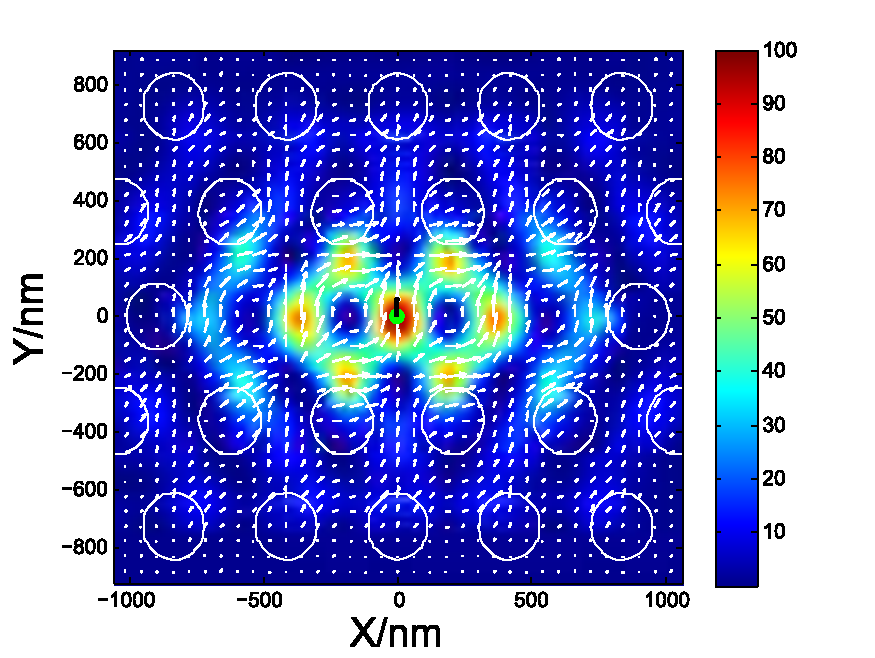
\includegraphics[width=16cm]{./Figs/dotsmode1_1}
\end{center}
\caption[Dipole and E-field distributions in a H3 PC cavity structure.]{\textbf{   Dipole and E-field distribution in a H3 PC cavity structure in the $z=0$ plane.}  The dipole (the green point) is polarized in y direction (see the black arrow) and is located at $[0,\, 0,\, 0]$ nm, which is the center of the cavity, with a strong y-polarized field. Color map and white arrows indicate relative strength and direction of the cavity field.}
\label{dotsmode1_1}
\end{figure}

\begin{figure}[H]
%\fontsize{18}{19}\selectfont
\centering
\begin{center}
%\psfrag{(w-w0)/meV}{$(\omega-\omega_c)/meV$}
\psfrag{realG}{real$\bG$}
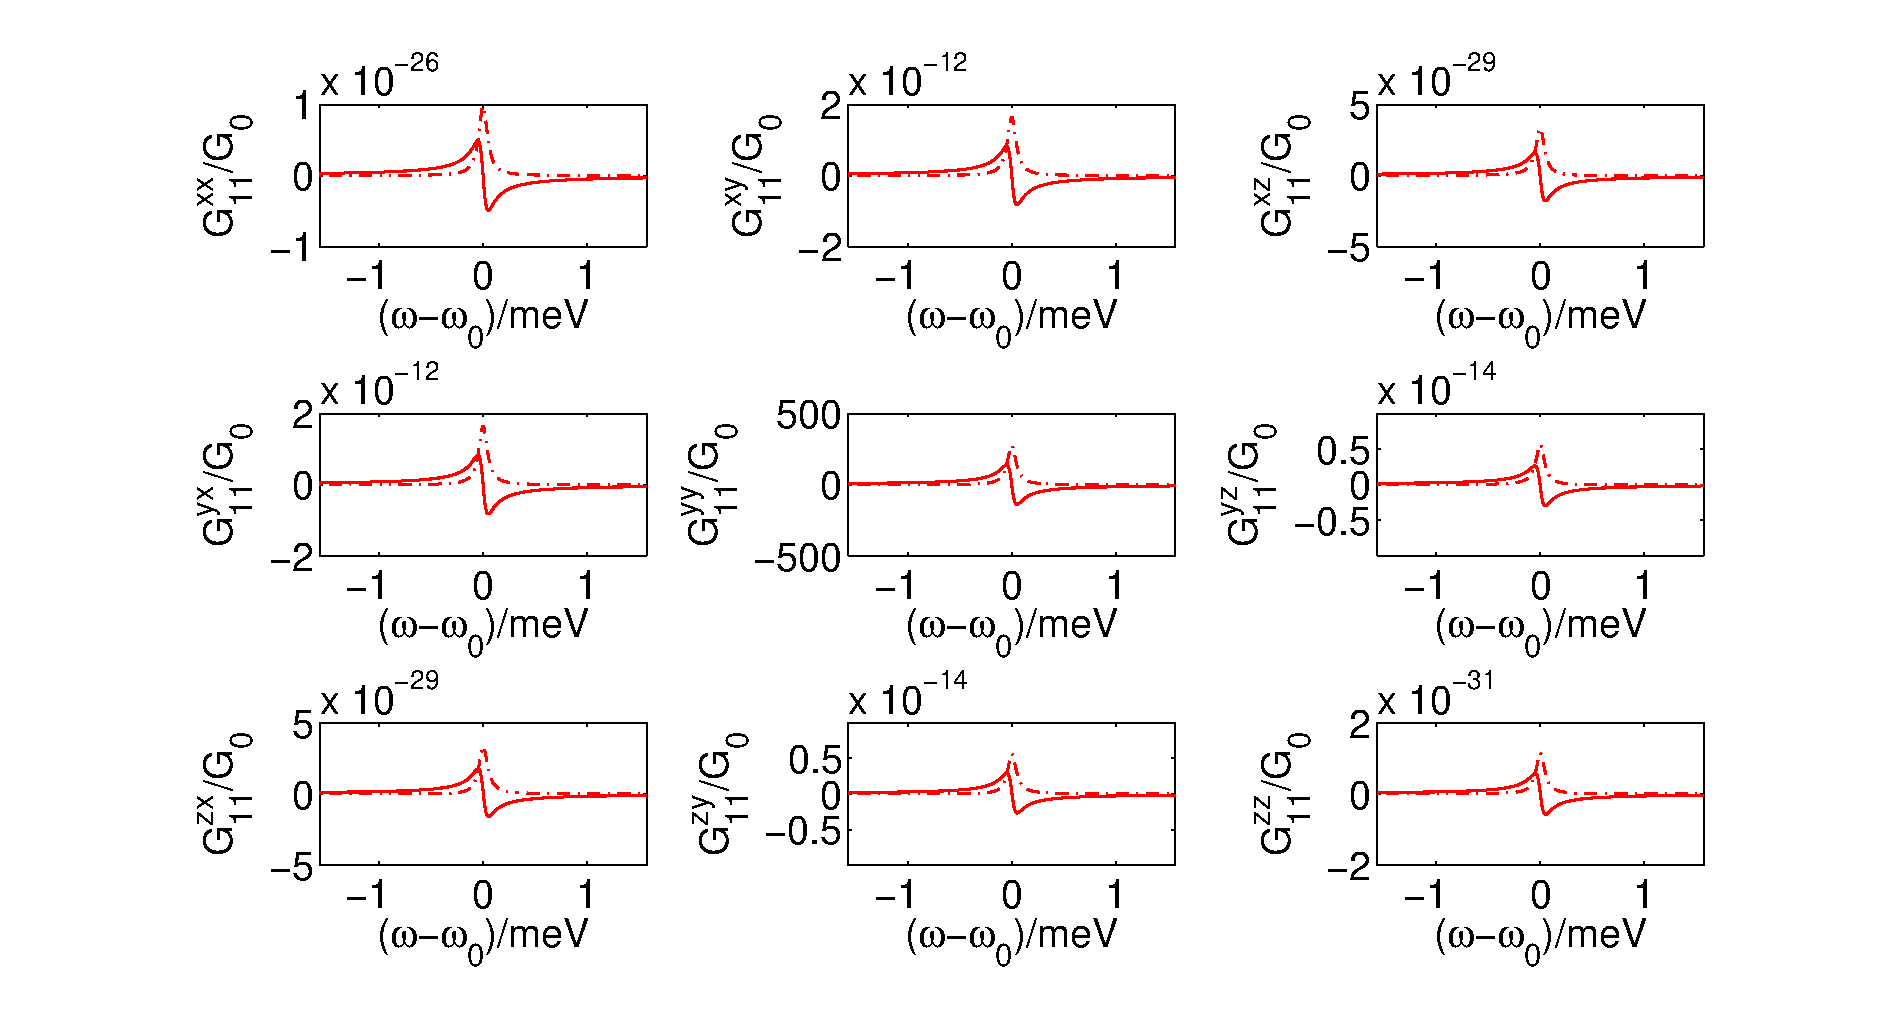
\includegraphics[width=16cm]{./Figs/G84_11_1}
\end{center}
\caption[Diagram of GFT tensor elements.]{\textbf{Full elements of $\mathbf{G}^0$ with $\omega_c/2\pi = 317 {\text {THz}}, \Gamma_c = 0.1 {\text {meV}}$ }. The $\mathbf{G}^{ij}_{11}$ is the $ij$-th component of the $\mathbf{G}^{(0)}(\br_1,\br_1,\omega)$. Dashed lines are the imaginary parts of the GFs; solid lines are the real parts of the GFs. All components are normalized to the homogeneous GF, $G_0$, given by Equ.\eqref{Ghom2}. As it shows, the $yy$ component dominates the GFT components.}
\label{G84_11_1}
%\normalsize
\end{figure}

\begin{figure}[H]
\centering
\begin{center}
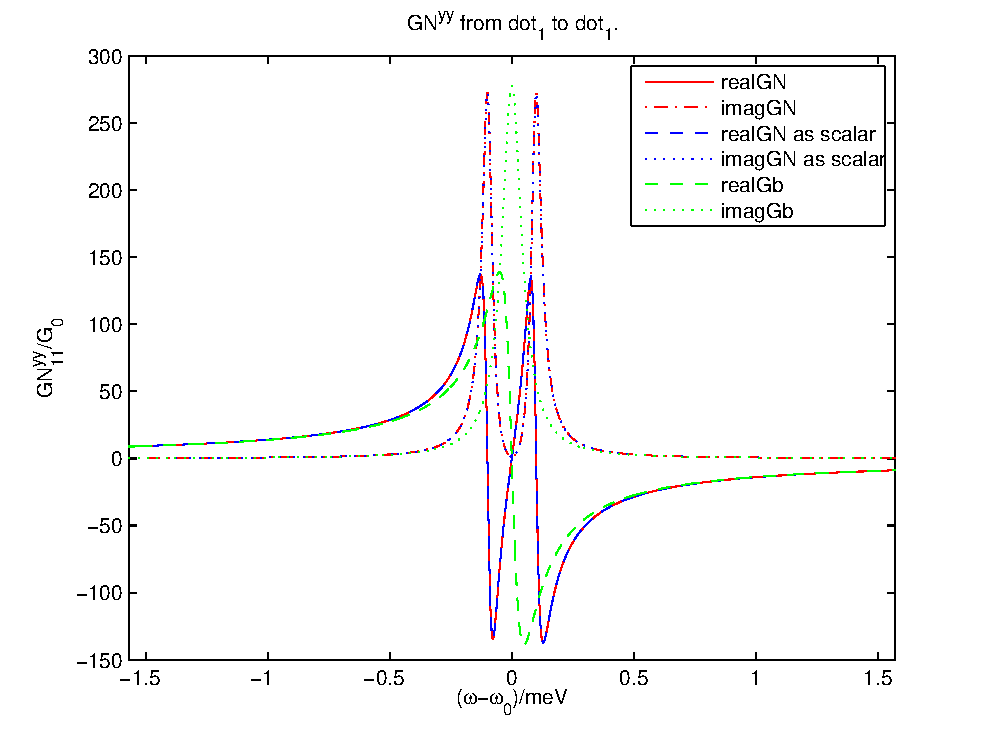
\includegraphics[width=14cm]{./Figs/G84_yy11_1}
\end{center}
\caption[yy component of $G^1(\mathbf{r}_1,\mathbf{r}_1)$ with an on-resonance dipole.]{\textbf{  yy component of $\mathbf{G}^1(\mathbf{r}_1,\mathbf{r}_1)$ with an on-resonance dipole of $\omega_d/2\pi = 317 {\text {THz}}, \Gamma_d = 2 \mu{\text {eV}}$ }. Red line shows the result calculated through full tensor iteration method; blue line is obtained by only considering y component of vectors through scalar iteration method; green line is bare cavity GF (yy-component) for comparison. Except for the bare cavity GF, all the other lines match up perfectly.}
\label{G84_yy11_1}
\end{figure}

\begin{figure}[H]
\centering
\begin{center}
\psfrag{dot}{dipole}
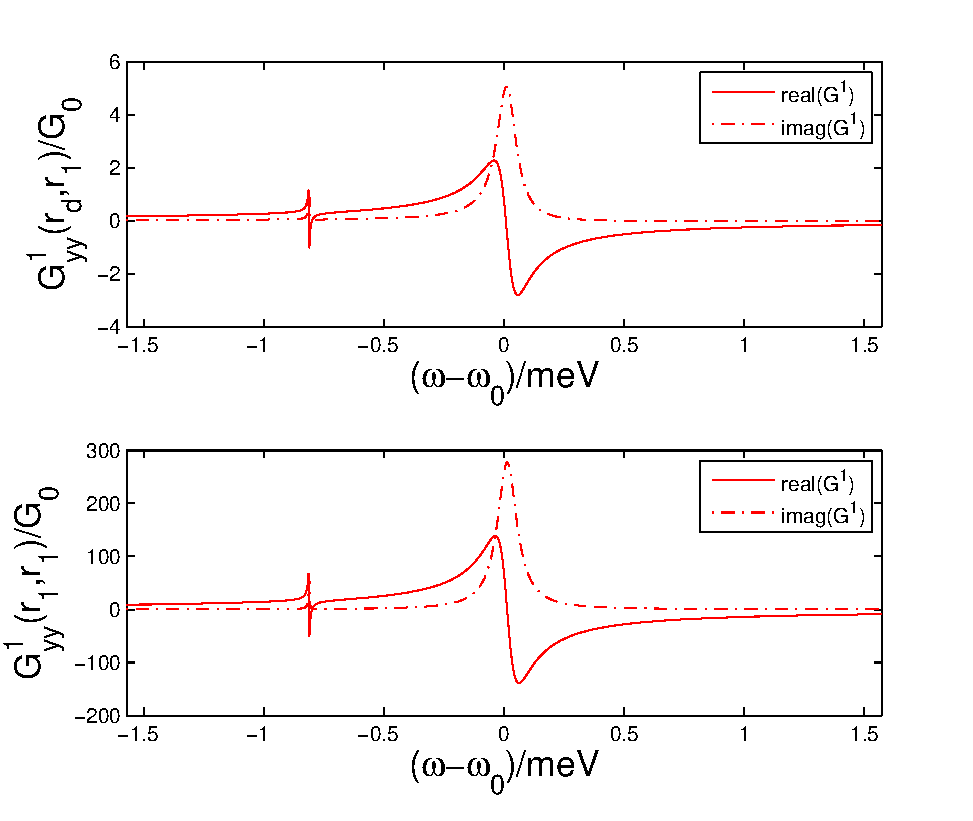
\includegraphics[width=14cm]{./Figs/G84_1yy_1}
\end{center}
\caption[yy component of GFT with an off-resonance dipole.]{\textbf{The yy components of $\bG^1(\mathbf{r}_d,\mathbf{r}_1)$ and $\bG^1(\mathbf{r}_1,\mathbf{r}_1)$  with an off-resonance dipole of $\Delta \omega = -0.8 {\text {meV}}, \Gamma_d = 2 \mu{\text {eV}}$ }. The upper plot shows the yy component detected at $\br_d=[0,\,0,\,420]$ nm above the cavity center; the bottom plot shows the yy component at the dipole responding to itself. Solid lines are the real parts of GFs. Dashed lines are the imaginary parts. }
\label{G84_1yy_1}
\end{figure}


\begin{figure}[H]
\centering
\begin{center}
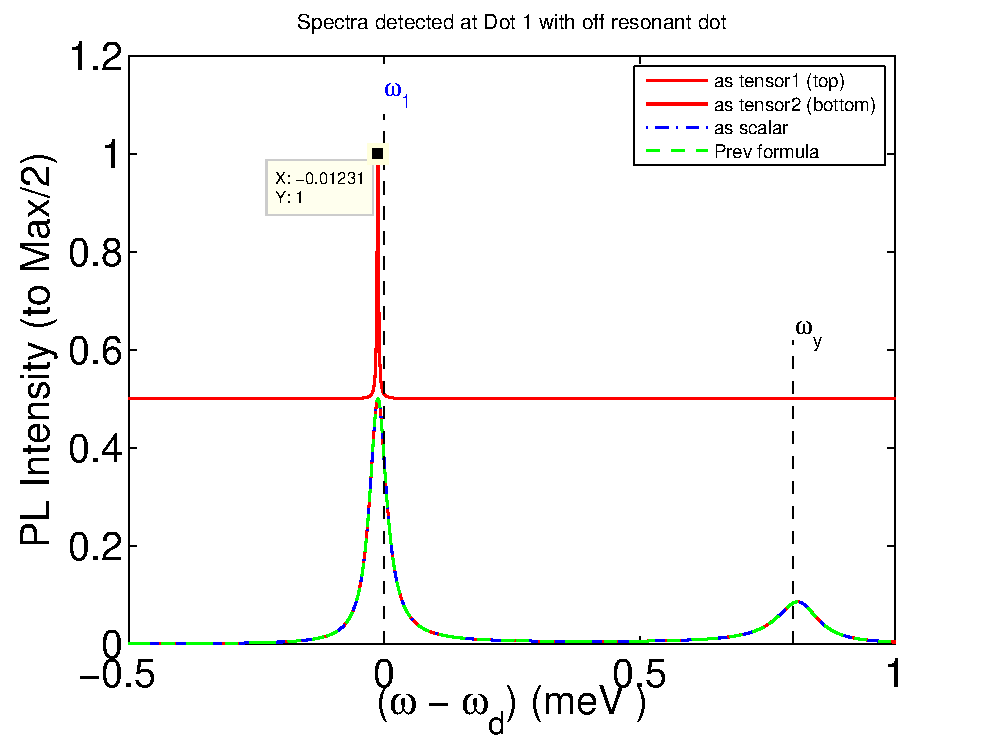
\includegraphics[width=14cm]{./Figs/sp84_11_1}
\end{center}
\caption[Spectra of off-resonance dipole in a PC cavity.]{\textbf{Spectra of off-resonance dipole in a PC cavity detected at the dipole position. $\Delta \omega = -0.8 {\text {meV}}$ }. $\omega_d$ is the dipole resonance; $\omega_y$ is the cavity resonance. $\Gamma_d = 2 \mu{\text {eV}}$ is used for the top plot; the bottom plot is with $\Gamma_d = 40 \mu{\text {eV}}$. For the bottom plot, the red, blue and green lines are obtained through full tensor method, scalar method (by only taking y component of dipole moment and $yy$ component of $\Gb$ into account) and according to the spectrum analytical formula given by Ref.~\cite{Hughes2009}. These three lines match up perfectly. The upper curves have be offset vertically by 0.5 for clarity. }
\label{sp84_11_1}
\end{figure}


\begin{figure}[H]
\centering
\begin{center}
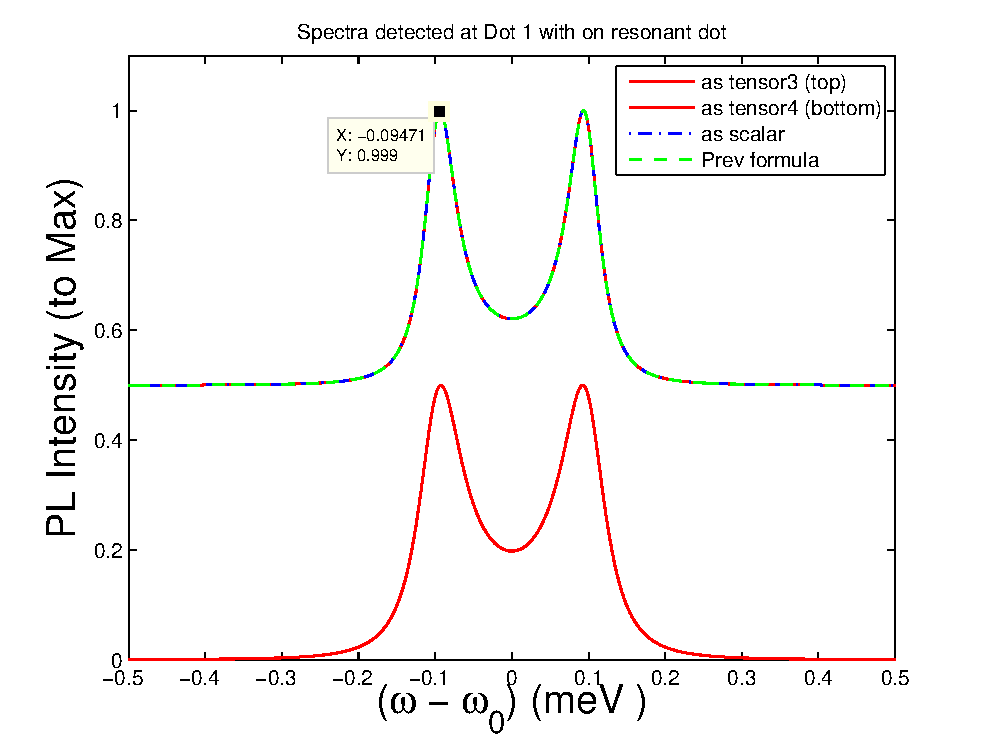
\includegraphics[width=14cm]{./Figs/sp84_11_2}
\end{center}
\caption[Spectra of a PC cavity with an on-resonance dipole.]{\textbf{Spectra of a PC cavity with an on-resonance dipole detected at the dipole position. $\Delta \omega = 0 {\text {meV}}$ }. Top lines are with a dipole decay rate of $\Gamma_d = 2 \mu{\text {eV}}$; bottom line is with $\Gamma_d = 40 \mu{\text {eV}}$. Notations are the same as Fig.~\ref{sp84_11_1}. Again, these three lines match up perfectly. There is an offset for 0.5 in the top curves for clarity.}
\label{sp84_11_2}
\end{figure}

\clearpage

\subsection{Cavity System with One $xy$-polarized Dipole}
As in the previous section, we still concentrate on one-dipole coupled cavity system,
but let us turn the dipole source's polarization direction at $45^\circ$ to the $x$ axis,
which means the polarization direction is between the $x$ and $y$ axes.
Now, the spectrum formula given by Ref.~\cite{Hughes2009} does not work for this case.
To further check the validity of the formula for the Green function in \cite{Hughes2009},
let us locate the dipole source at a place where both x and y components of the E-field contribute to the cavity GFT,
which leads to a ``non-diagonal'' GFT as a result.
And in this case, we cannot only use $yy$ component of GFT to analyze the spectrum.
%All graphs in this section are returned from code SpecPC\_1.m version 13 in Test file of GFT project repository.

The dipole location and polarization direction is shown in Fig.\ref{dotsmode1_2}
\begin{figure}[H]
\centering
\begin{center}
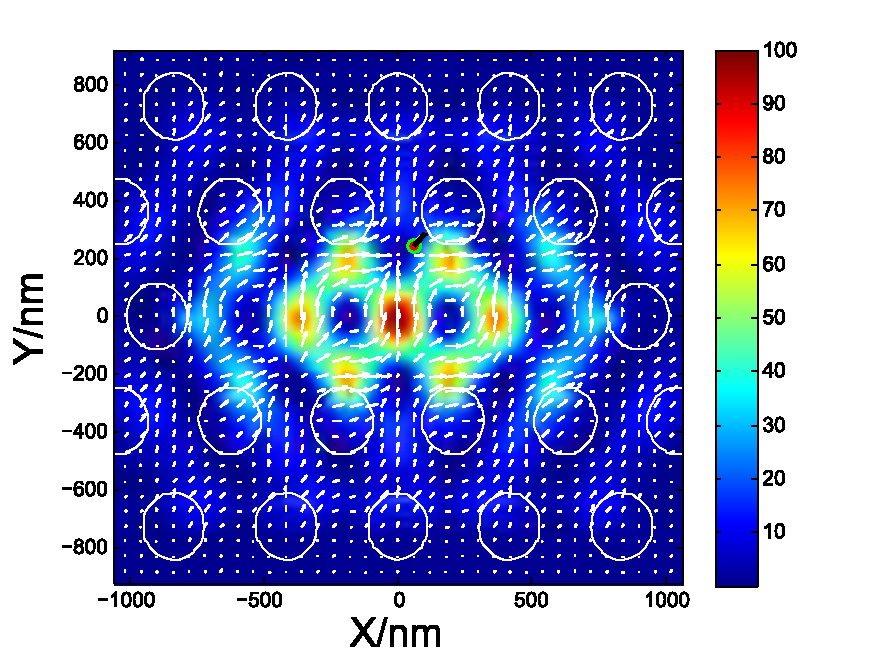
\includegraphics[width=14cm]{./Figs/dotsmode1_2}
\end{center}
\caption[Dipole and E-field distributions in a H3 PC cavity structure.]{\textbf{  Dipole and E-field distribution in a H3 PC cavity structure in $z=0$ plane.}  The dipole (indicated by the red point) polarizes in the x-y direction (see the black arrow at the dipole) and is located at $[60,100\times\sqrt{3}+60,\, 0]$ nm, where the E-field of the cavity has both x and y components. The color map corresponds to the relative strength of the cavity mode, and white arrows indicate on-site E-field vectors.}
\label{dotsmode1_2}
\end{figure}
The GFT elements for this bare cavity are shown in Fig.\ref{G84_11_4}.
\begin{figure}[H]
\centering
\begin{center}
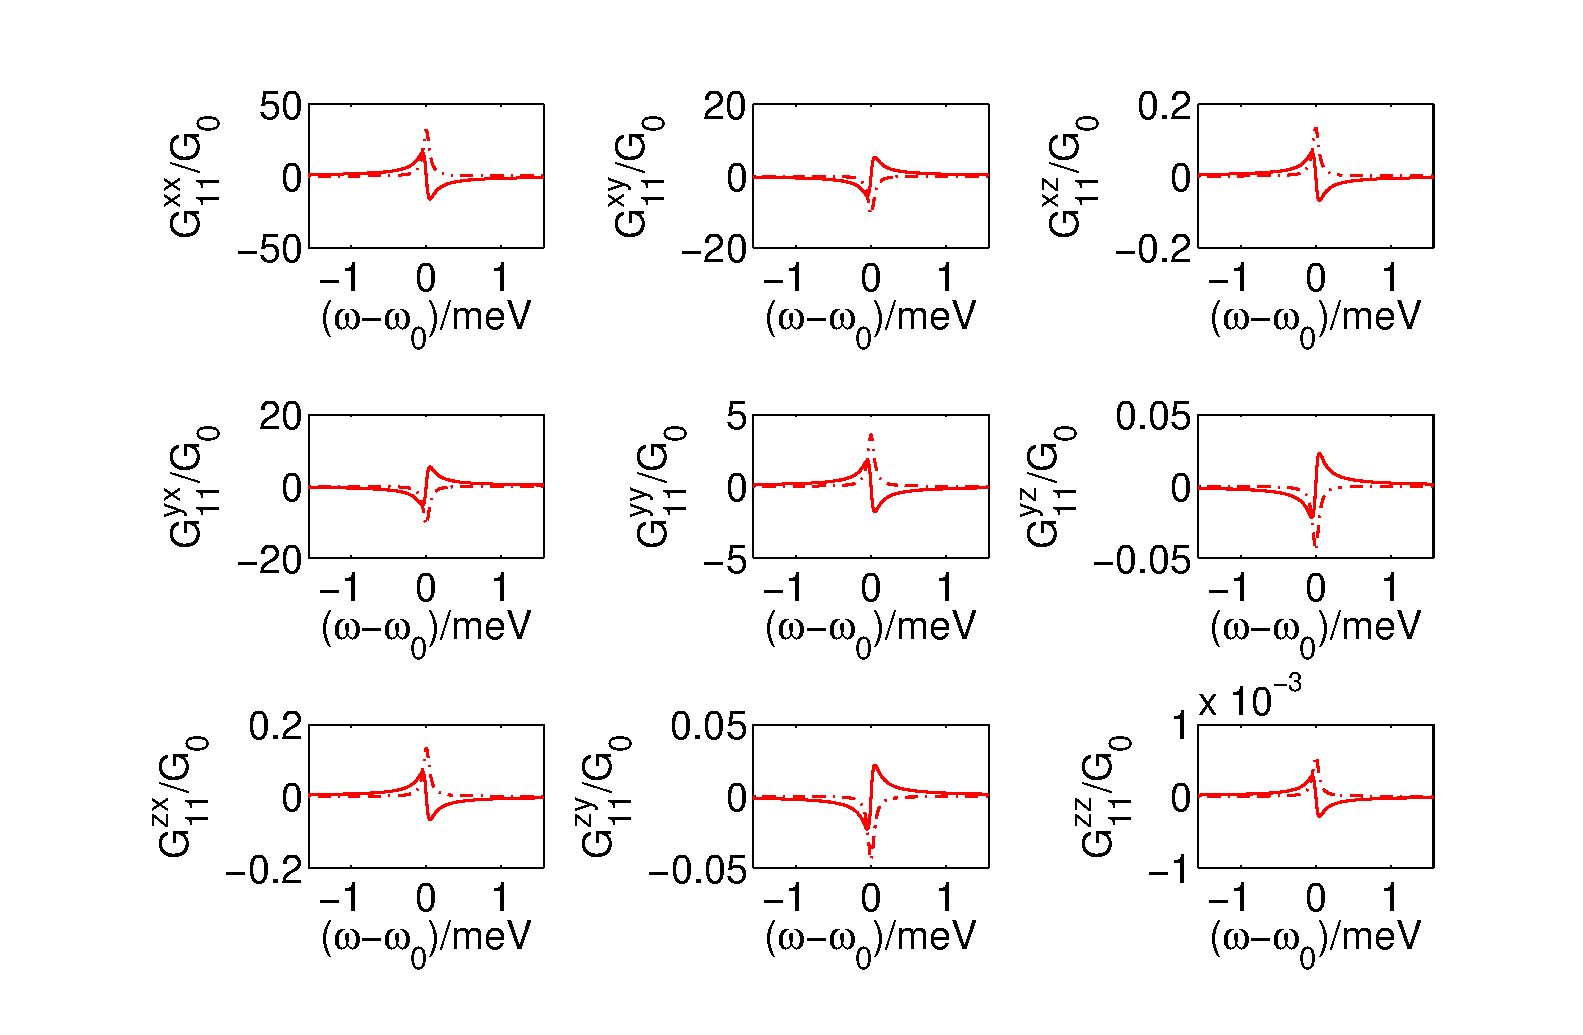
\includegraphics[width=16cm]{./Figs/G84_11_4}
\end{center}
\caption[Full elements of $G^0$ with $\omega_c/2\pi = 317 {\text {THz}} (\lambda_c=945 {\text {nm}}), \Gamma_c = 0.1 {\text {meV}}$]{\textbf{Full elements of $G^0$ with $\omega_c/2\pi = 317 {\text {THz}} (\lambda_c=945 {\text {nm}}), \Gamma_c = 0.1 {\text {meV}}$ }. The source locates at  $\br_1=[60,100\sqrt{3}+60,\, 0]$ nm (see Fig.~\ref{dotsmode1_2}) with both large x and y components of GFT. The $\mathbf{G}^{ij}_{11}$ is the $ij$-th component of the $\mathbf{G}^{(0)}(\br_1,\br_1,\omega)$. Dashed lines are the imaginary part of the GFs; solid lines are the real parts of the GFs. All components are normalized to the homogeneous GF, $G_0$, given by Equ.\eqref{Ghom2}. }
\label{G84_11_4}
\end{figure}

The $yy$ component of the total GFT for this 1-dipole system is shown in Fig.\ref{G84_1yy_2}. Compared with the scalar computational method, which only takes the $yy$ component of $\Gb$ and $y$ component of dipole moment into account, the full tensor calculation shows a cross-coupling effect from the $x$ component.
\begin{figure}[H]
\centering
\begin{center}
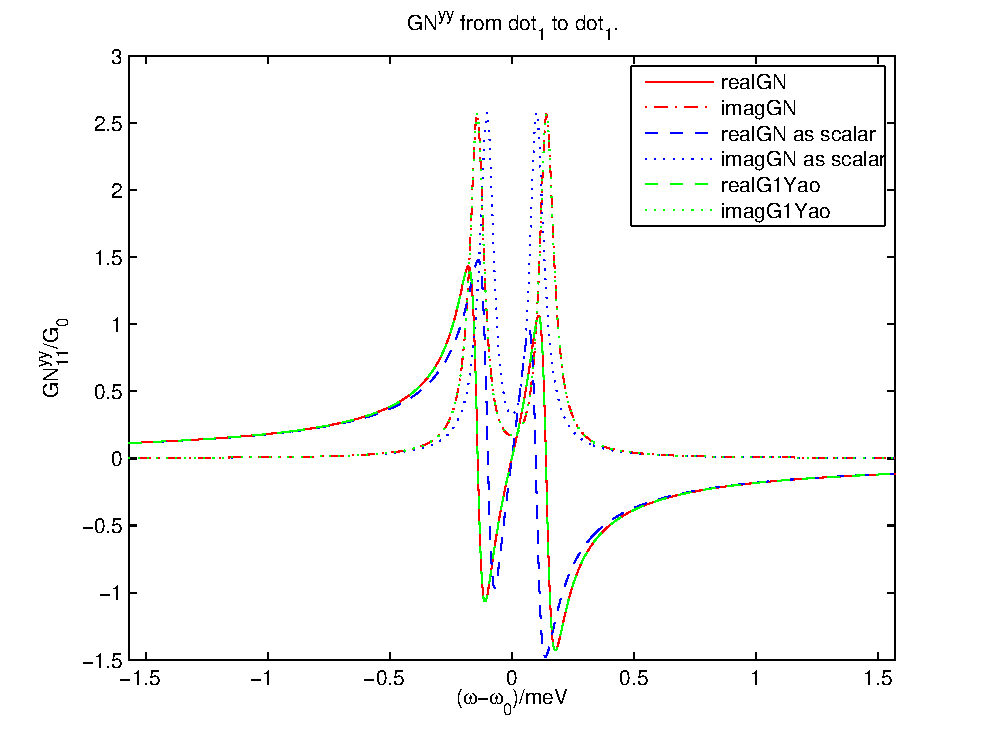
\includegraphics[width=14cm]{./Figs/G84_1yy_2}
\end{center}
\caption[yy component of $G^1(\mathbf{r}_1,\mathbf{r}_1)$  with one on-resonance dipole.]{\textbf{  yy component of $G^1(\mathbf{r}_1,\mathbf{r}_1)$  with one on-resonance dipole}. Red lines show the full tensor calculation of the real and imaginary parts of the yy component at dipole 1; blue lines show the scalar calculation of GF at dipole 1 responding to itself, by only taking the yy component of $\Gb$ and y component of dipole moment into account; green lines show the results of one-dipole GFT with scalar denominator as described in Appendix~\ref{section:GFscalar}~\cite{Yao2009b} for comparison. Now we can see the blue line does not match with other lines. This is because both $yx$ and $xy$ components of $\Gb$ play roles in the GFT calculation, and the tensor algebra cannot be simplified as a scalar algebra since the cross-coupling effect becomes evident. While the red and green lines agree very well. This shows the equivalence of these two theories.}
\label{G84_1yy_2}
\end{figure}

For the cases we have studied in the last subsection above, if the dipole source is polarized to neither $x$ nor $y$ direction, the spectra show that making the denominator to be a scalar in the total GFT expression is equivalent to the full tensor treatment (see Appendix~\ref{section:GFscalar}). As an example to exam different GF calculation methods, the $x$- and $y$-polarized spectra for off- and on-resonance cases are shown in Fig.\ref{sp84_11_7x}, and Fig.\ref{sp84_11_7y}. The plots in the two figures show that the iterative and non-iterative methods and the method presented in Appendix~\ref{section:GFscalar}~\cite{Yao2009b} are equivalent.
\begin{figure}[H]
\centering
\begin{center}
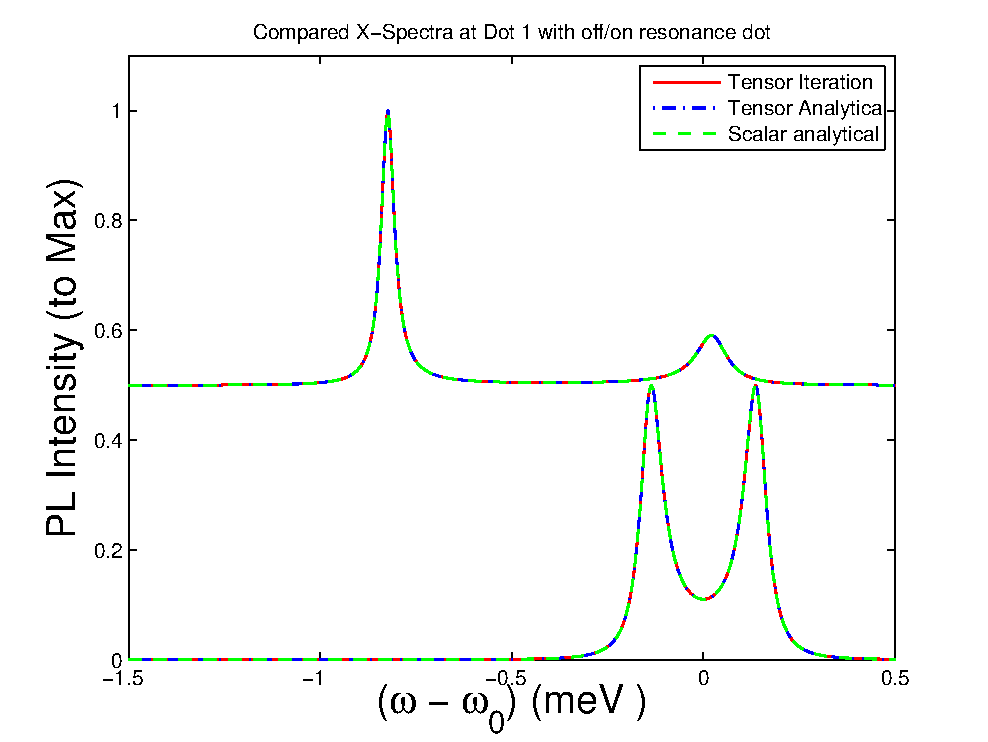
\includegraphics[width=14cm]{./Figs/sp84_11_7x}
\end{center}
\caption[X component of Spectra of off-resonance and on-resonance dipoles.]{\textbf{  X component of Spectra of off-resonance (top) and on-resonance (bottom) dipoles in the PC cavity, detected at the dipole position, with dipole decay rate of $\Gamma_d = 40 \mu{\text {eV}}$ }. Top lines are with a detuning $\Delta \omega = -0.8 {\text {meV}}$. Red lines are obtained through full tensor iteration method; blue lines are obtained through full tensor non-iteration analytical expression in Appendix~\ref{section:noniterativeGF}; green lines are based on the GFT calculation method reported in Ref.~\cite{Yao2009b} or Appendix~\ref{section:GFscalar}. The amplitudes are normalized to the maximum of the absolute value of the PL spectrum. The top curves are offset by 0.5 for clarity.}
\label{sp84_11_7x}
\end{figure}

\begin{figure}[H]
\centering
\begin{center}
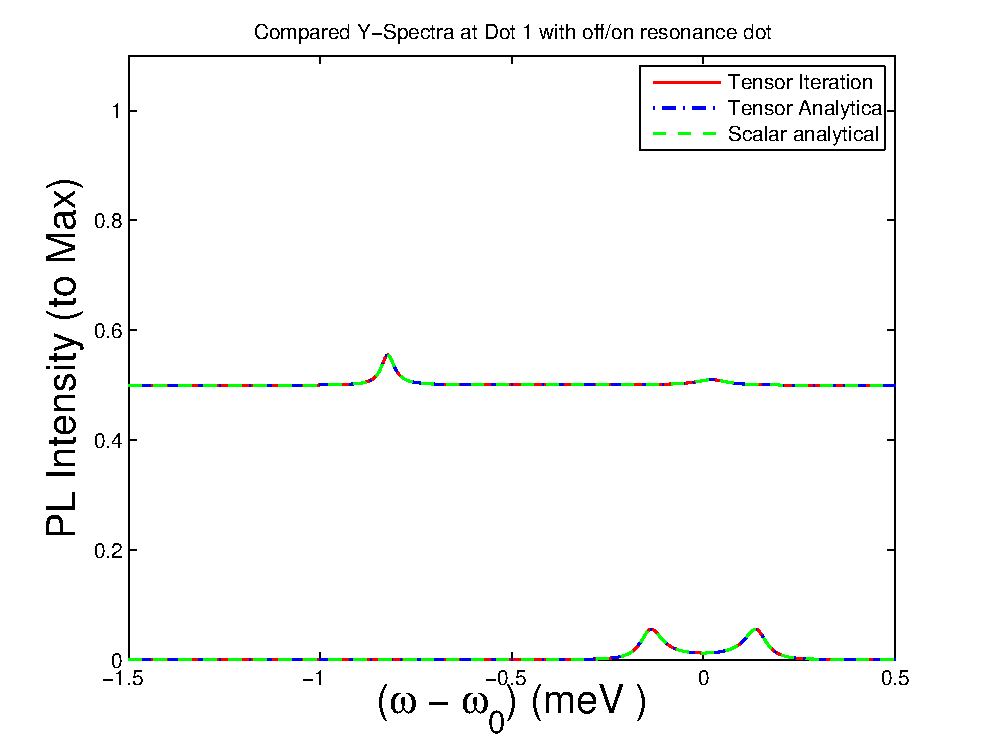
\includegraphics[width=14cm]{./Figs/sp84_11_7y}
\end{center}
\caption[Y component of Spectra of off-resonance and on-resonance dipoles.]{\textbf{  Y component of Spectra of off-resonance (top) and on-resonance (bottom) dipoles in a PC cavity}. Notation and calculation methods are the same as Fig.~\ref{sp84_11_7x}. The top curves are offset by 0.5 for clarity.}
\label{sp84_11_7y}
\end{figure}


%\clearpage

\subsection{Two-dipole coupled cavities}
\subsubsection{Two-dipole system with $y$-polarized sources}
In this part, we will demonstrate the spectrum of the two-dipole coupled cavity.
Results will be compared with those of Ref.~\cite{Yao2009c}.
%The testing code is located at GFT tool box repository/Test with a name SpecPC\_2.m (version 7, but need to change en to be [0,1,0] in the code).
The parameters used are as follows:
%\begin{equation}
\begin{align}
 \omega_c/2\pi = \omega_{1(2)}/2\pi &= 191.551 {\text {THz}},\\
 \Gamma_c &= 20.2 \mu{\text {eV}}, \\
 d_{1(2)} &= 30 {\text {Debye}}, \\
 \Gamma_{d1(2)} &= 2 \mu{\text {eV}}, \\
 g_1 = 0.0564 {\text {meV}}, &\quad g_2=0.0230 {\text {meV}}.
\end{align}
%\end{equation}
These two dipoles are located at $\br_1=[0,0,0]$ nm and $\br_2=[0,190*\sqrt{3},0]$ nm, where the origin is the center of the cavity (Fig.\ref{dotsmode2_1}). We use $\omega_{1 (2)}$ indicating the dipole 1(2)' resonance, which is on-resonance. $d_{1(2)}$ and $\Gamma_{d1(2)}$ are the optical moment and decay rate of dipole 1(2), respectively. $g_1$ and $g_2$ are the coupling strengths of the two dipoles based on Equ.\eqref{eq:g1}. The $yy$ component of the total GFT for this system is shown in Fig.\ref{G84_2yy11_1}. Comparisons among different calculation methods for the spectrum are shown in Figs.~\ref{sp84_11_3} and~\ref{sp84_11_4}. All plots agree with each other very well, and show the splitting feature of the strong coupled dipoles-cavity system.

We notice that, when the two dipoles are both on-resonance, the spectral splitting width is less than $2(g_1+g_2)$, and differs from $2g_1$ or $2g_2$ (see the labels in Figs.~\ref{sp84_11_3} and~\ref{sp84_11_4}). This feature implies that the total coupling strength with two dipoles is not simply the sum of two individual dipole-cavity coupling strengths. Theoretical and experimental studies on identical on-resonance dipoles coupled to a homogeneous field of a cavity confirm that the spectral splitting width are $\sqrt{N}g$, where $g$ is the coupling strength of an individual dipole to the cavity, and $N$ is the number of the dipoles~\cite{Kimble1998,Tischler2007}; in the case above, however, the spectral splitting width cannot be predicted by the $\sqrt{N}g$ relationship, since the dipoles do not share the same coupling strength.  Moreover, we also notice that the splitting width of the spectrum (in Fig.~\ref{sp84_11_3}) is different from that of imaginary part of the GFs ($yy$ component of the $\mathbf{G}^2(\mathbf{r}_1,\mathbf{r}_1)$ in Fig.~\ref{G84_2yy11_1}) as Equ.\eqref{eq:sN_mixedstate_withdecay} defines.
\begin{figure}[H]
\centering
\begin{center}
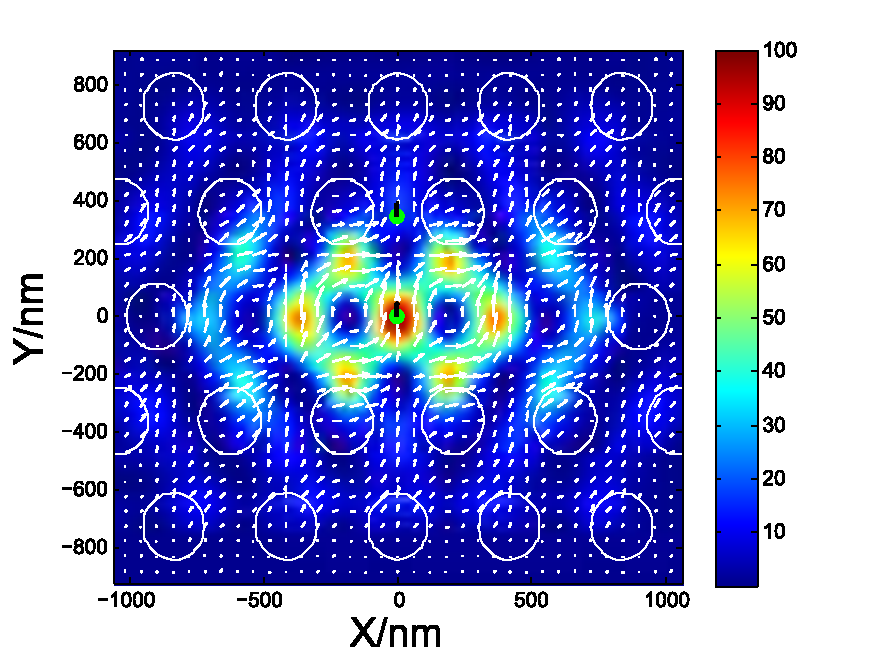
\includegraphics[width=14cm]{./Figs/dotsmode2_1}
\end{center}
\caption[Dipoles and E-field distribution in a H3 PC cavity structure.]{\textbf{  Dipoles and E-field distribution in a H3 PC cavity structure in $z=0$ plane.}  The dipoles (indicated by green points) both polarize in the y direction (see the black arrows), and is located at $[0,\, 0,\, 0]$ nm (the center of the cavity with a strong y-mode) and $[0,\, 190\sqrt{3},\, 0]$ nm. The color map corresponds to the relative strength of the cavity mode. White arrows indicate on-site E-field vectors.}
\label{dotsmode2_1}
\end{figure}


\begin{figure}[H]
\centering
\begin{center}
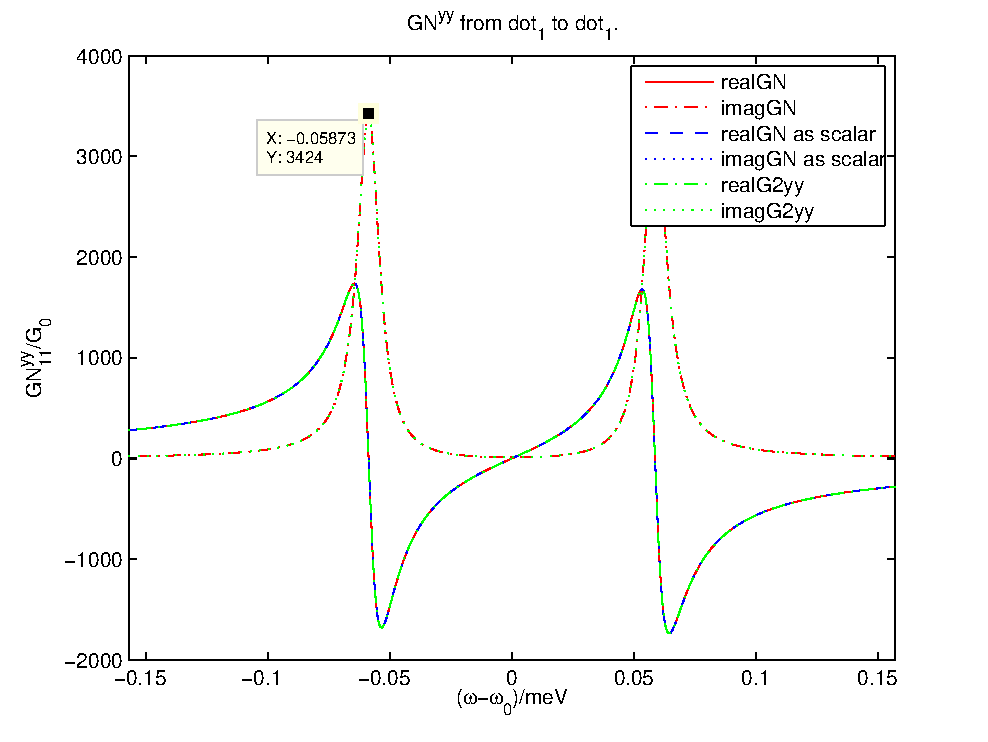
\includegraphics[width=14cm]{./Figs/G84_2yy11_1}
\end{center}
\caption[yy component of $G^2(\mathbf{r}_1,\mathbf{r}_1)$  with two on-resonance dipoles.]{\textbf{$yy$ component of $\mathbf{G}^2(\mathbf{r}_1,\mathbf{r}_1)$  with two on-resonance dipoles of $\Gamma_d = 2 \mu{\text {eV}}$ }. Red lines are obtained by using the full tensor calculation method; blue lines are from the scalar calculation with yy component of $\Gb$ and $y$ component of dipole moment; green lines are the result of the analytical formula in Ref.~\cite{Yao2009c}. These lines are on top of each other. }
\label{G84_2yy11_1}
\end{figure}


\begin{figure}[H]
\centering
\begin{center}
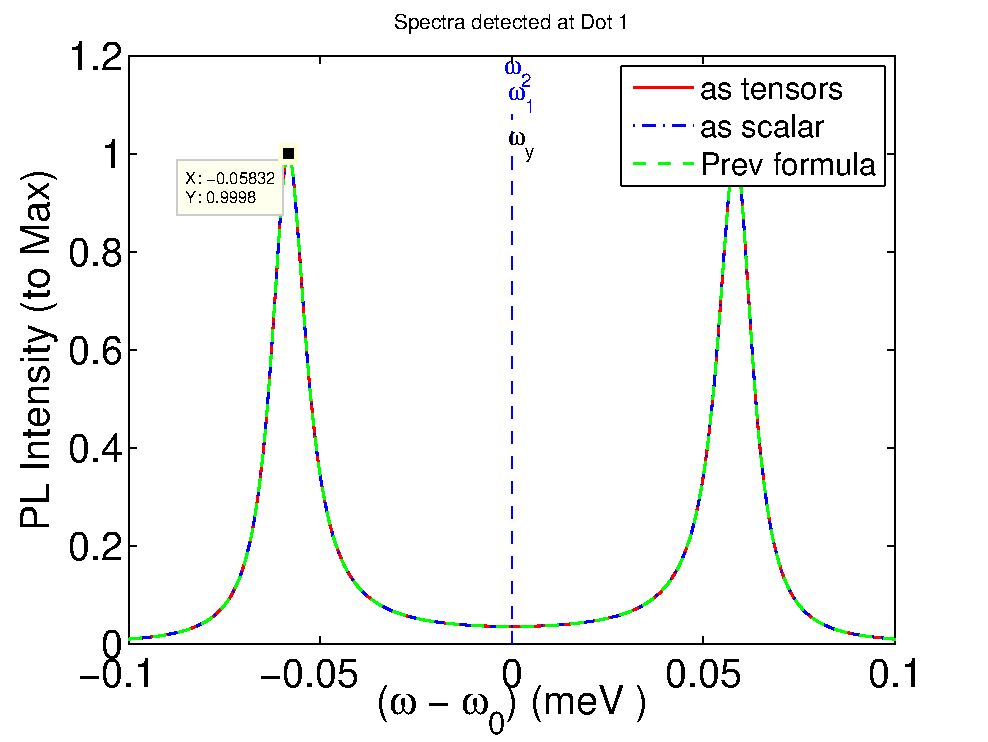
\includegraphics[width=14cm]{./Figs/sp84_11_3}
\end{center}
\caption[Spectra of on-resonance dipoles, with three calculation methods.]{\textbf{Spectra of on-resonance dipoles in a PC cavity, calculated with three methods}. $\omega_y=\omega_0$ is the cavity resonance. Red line is obtained through iterative full tensor method; blue line is obtained through scalar method, by only taking account the $yy$ component of $\Gb$ and $y$ component of dipole moment; green line is the result of the formula in Ref.~\cite{Yao2009c}. These lines are on top of each other.}
\label{sp84_11_3}
\end{figure}


\begin{figure}[H]
\centering
\begin{center}
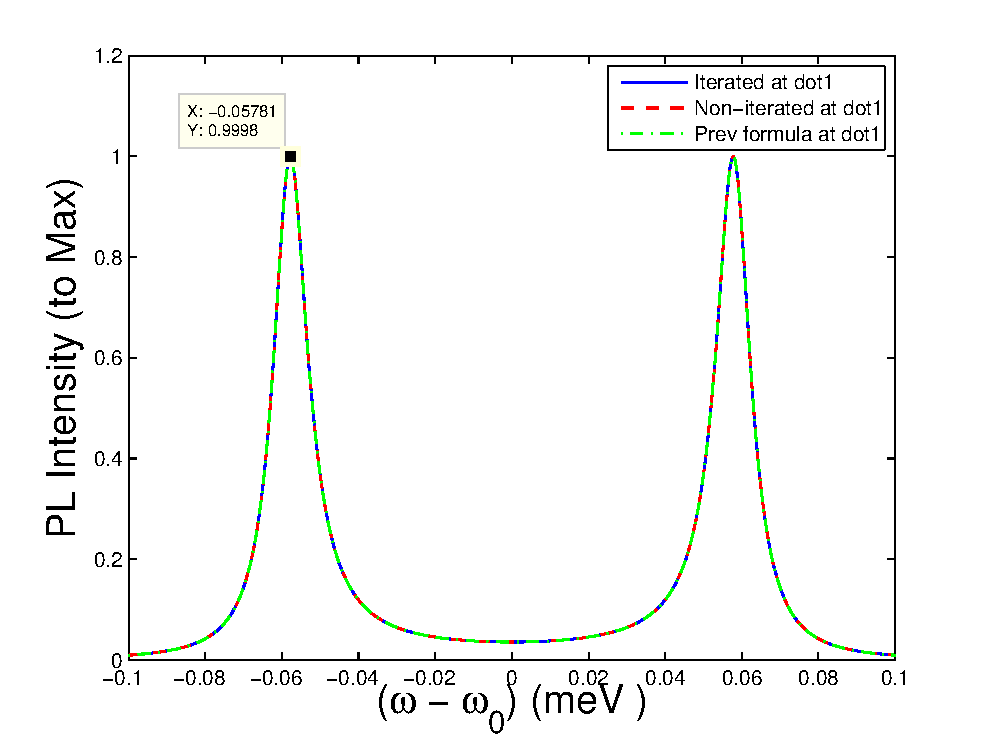
\includegraphics[width=14cm]{./Figs/sp84_11_4}
\end{center}
\caption[Spectra of on-resonance dipoles, based on three analytical expressions.]{\textbf{Spectra of on-resonance dipoles in PC cavity detected at dipole 1 based on three analytical expressions}. Red line is plotted according to full tensor iterative analytical expression in Appendix~\ref{App:GF}; blue line is obtained through non-iterative analytical expression in Appendix~\ref{App:GF}; green line is plotted based on the analytical formula for $G^2$ in Ref.~\cite{Yao2009c}. Again, these three lines are on top of each other.}
\label{sp84_11_4}
\end{figure}

%\clearpage

\subsubsection{Cavity System with Two $xy$-polarized Dipoles}
In this section, we will turn both the dipoles' polarization directions to $45^\circ$ up $x$ axis,
which means the dipoles are polarized between $x$ and $y$ axes.
We locate the dipole sources to places where both $x$ and $y$ components of E-field contribute to the GFT (Fig.~\ref{dotsmode2_2}). Now, the GFT of the bare cavity is non-diagonal (Fig.~\ref{G84_11_2}).
%In this case, we cannot only use $yy$ components of GFTs to analyze the spectrum.
%All graphs in this section are returned from code SpecPC\_2.m version 13 in Test file of GFT project repository.

The $yy$ component of total GFT for this two-dipole system is shown in Fig.~\ref{G84_2yy11_2}. Comparisons of spectra calculated from different methods are shown in Figs.~\ref{sp84_11_5} and~\ref{sp84_11_6}. Again, the cross-coupling effect of the $x$ and $y$ components is evident.

We also notice that the coupling strengths of the two dipoles are $g_1=0.0268$ meV and $g_2=0.0363$ meV; the width of the splitted spectral peaks when the two dipoles are on-resonance is $2\times 0.01107$ meV, which is less than both $2g_1$ and $2g_2$. Similar to the solely $y$-polarized case discussed in the last subsection, again, we observed the complicated combination of two dipoles coupling to a cavity. In both cases, we employed the separation of doublets to be the spectral splitting width. In Chapter~\ref{ch:ensemble}, we will use the FWHM as the general description quantity to measure how the spectrum is broadened or narrowed.

The spectral behaviors (shifting and broadening) with more than two dipoles will be discussed in the next section and the next chapter.
\begin{figure}[H]
\centering
\begin{center}
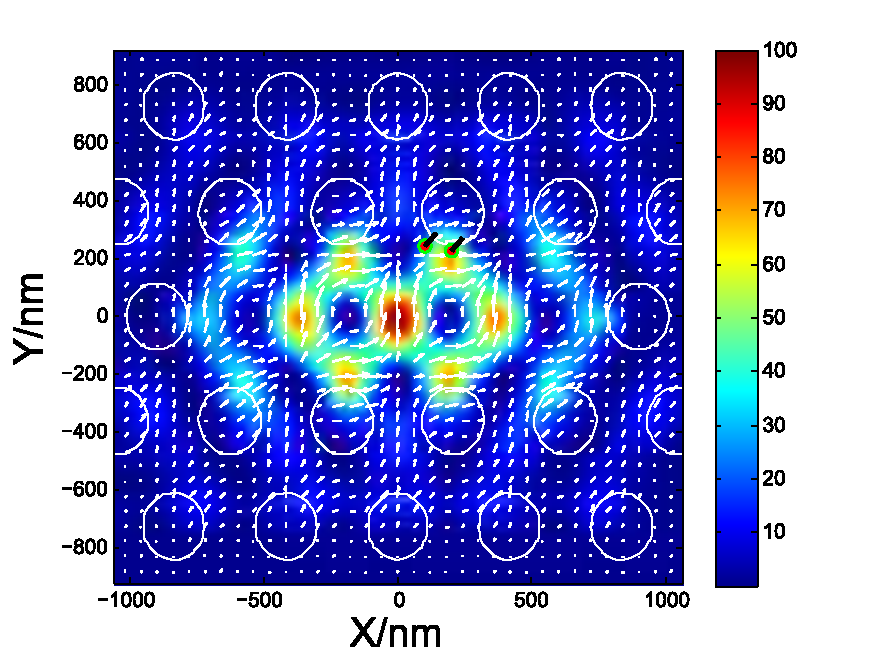
\includegraphics[width=14cm]{./Figs/dotsmode2_2}
\end{center}
\caption[Dipole and E-field distribution in a H3 PC cavity structure.]{\textbf{  Dipoles and E-field distribution in a H3 PC cavity in the $z=0$ plane.}  The dipoles (red points) polarize to x-y direction (see the black arrows at the dots) and locate at $\mathbf{r}_1=[100,\, 240,\, 0]$ nm and $\mathbf{r}_2=[200,\, 100\sqrt{3}+40, \, 0]$ nm, where the E-fields have both x and y components. Color map corresponds to relative strength of the cavity mode, and white arrows indicate on-site E-field vectors.}
\label{dotsmode2_2}
\end{figure}

\begin{figure}[H]
\centering
\begin{center}
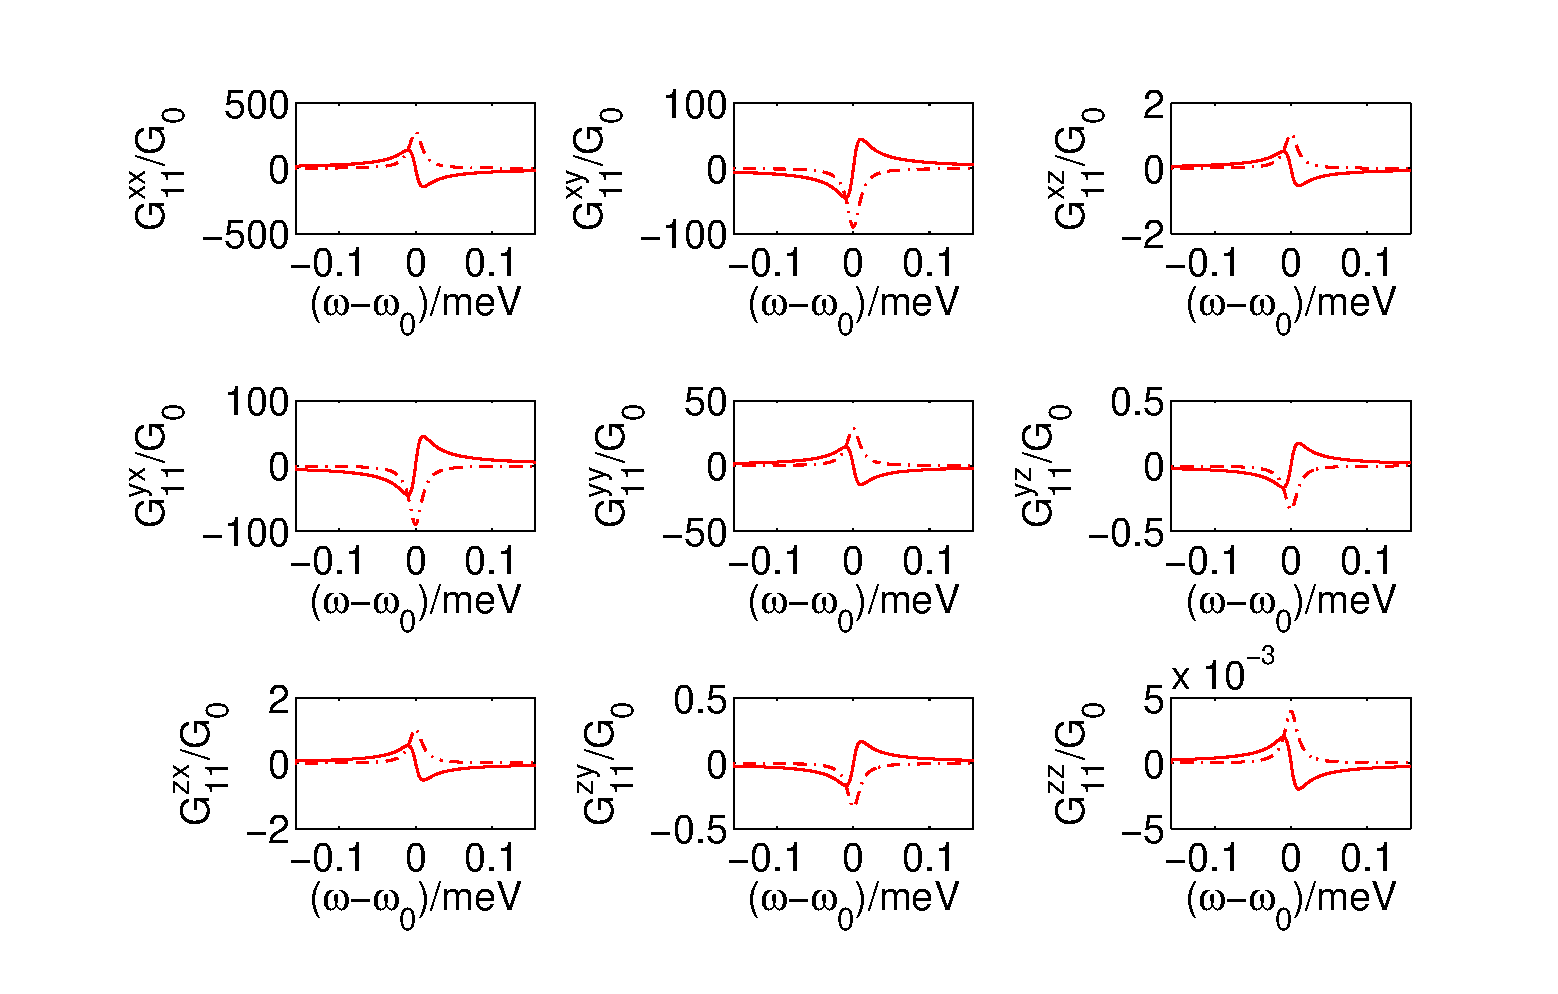
\includegraphics[width=16cm]{./Figs/G84_11_2}
\end{center}
\caption[Full elements of $G^0(\mathbf{r}_1,\mathbf{r}_1)$.]{\textbf{Full elements of $G^0(\mathbf{r}_1,\mathbf{r}_1)$. $\omega_c/2\pi = 191.155 {\text {THz}},\, \Gamma_c = 0.010 {\text {meV}}$ }. The $\mathbf{G}^{ij}_{11}$ is the $ij$-th component of the $\mathbf{G}^{(0)}(\br_1,\br_1,\omega)$. Dashed lines are the imaginary part of the GFs; solid lines are the real parts of the GFs. All components are normalized to the homogeneous GF, $G_0$ (Equ.\eqref{Ghom2}).}
\label{G84_11_2}
\end{figure}


\begin{figure}[H]
\centering
\begin{center}
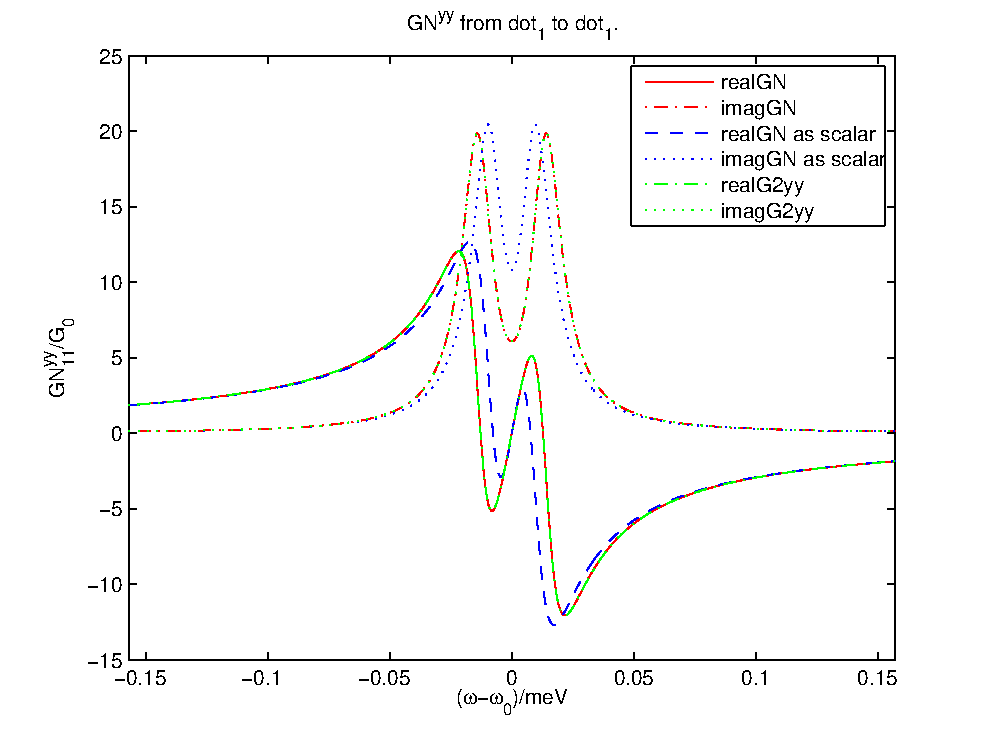
\includegraphics[width=14cm]{./Figs/G84_2yy11_2}
\end{center}
\caption[yy component of $G^2(\mathbf{r}_1,\mathbf{r}_1)$  with two on-resonance dipoles.]{\textbf{  yy component of $G^2(\mathbf{r}_1,\mathbf{r}_1)$  with two on-resonance dipoles. $\Gamma_d = 2 \mu{\text {eV}}$ }. Red lines show the full tensor calculation result; blue lines show the scalar calculation result; green lines are from the analytical formula in Ref.\cite{Yao2009c}. The blue line does not agree with others. This is because the bare cavity GFT cannot be simplified as a scalar. The red and green lines match up perfectly.}
\label{G84_2yy11_2}
\end{figure}


\begin{figure}[H]
\centering
\begin{center}
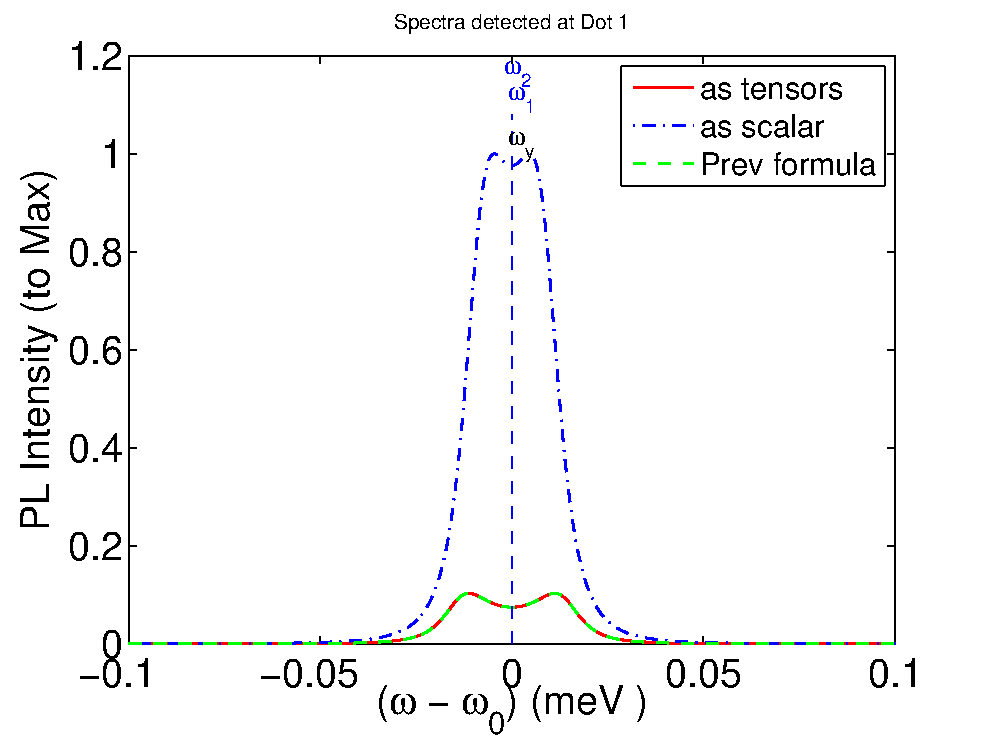
\includegraphics[width=14cm]{./Figs/sp84_11_5}
\end{center}
\caption[Spectra of on-resonance dipoles, with three calculation method.]{\textbf{Comparison of three calculation methods for the spectra with two on-resonance dipoles in a PC cavity.} Red line is obtained through full tensor method; blue line is obtained through only taking the yy component of the bare cavity GFT and the y component of the dipole moment into account; green line is from the analytical formula in Ref~\cite{Yao2009c} by making the denominator a scalar. Except for the blue line, other lines agree with each other perfectly. Lines are normalized to the maximum of the blue line.}
\label{sp84_11_5}
\end{figure}


\begin{figure}[H]
\centering
\begin{center}
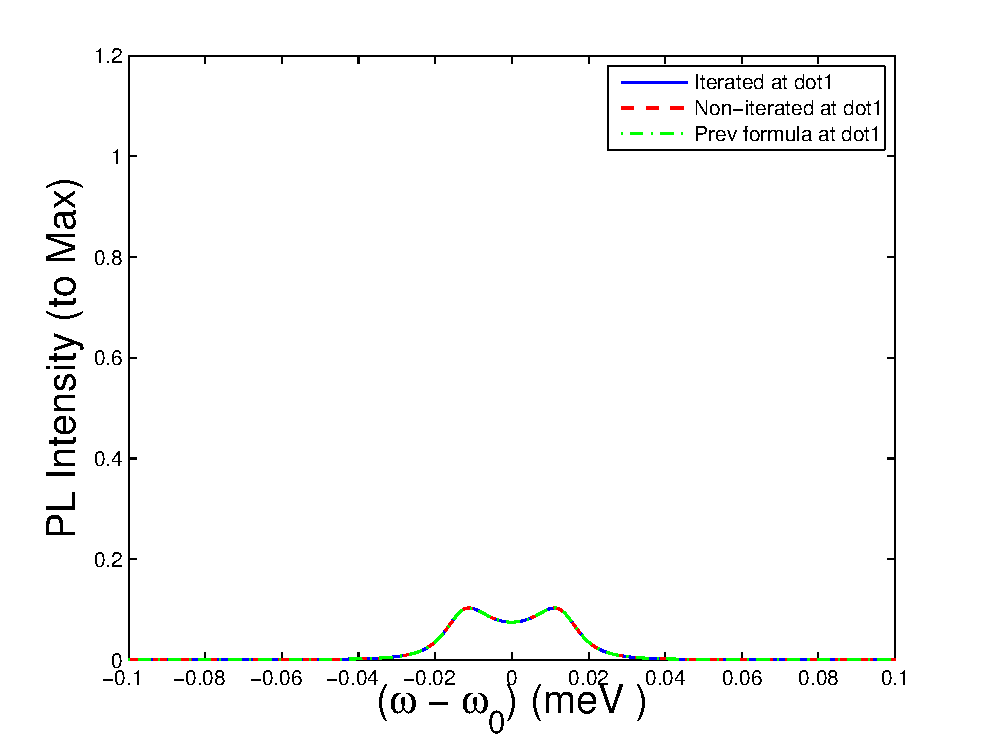
\includegraphics[width=14cm]{./Figs/sp84_11_6}
\end{center}
\caption[Spectra of on-resonance dots, based on three analytical expressions.]{\textbf{Comparison of spectra of on-resonance dipoles in a PC cavity from three analytical expressions}. The red, blue and green lines are obtained from the full tensor iterative, non-iterative analytical expressions (Appendix~\ref{App:GF}) and the analytical formula in Ref~\cite{Yao2009c}, repectively. These three lines agree with each other very well. With the same scale as Fig.~\ref{sp84_11_5}.}
\label{sp84_11_6}
\end{figure}

\subsection{Summary}
In this section, we studied the cavity spectral behaviors under the interaction with one or two dipoles. We observed a slight spectral shift effect in the presence of dipoles. We also observed the spectrum is affected by the width, coupling strength and position of the dipoles. Especially, when there are more than one dipoles in the cavity, the spectrum is complicated. As an example, the on-resonance two dipoles coupled cavity is studied in detail.

As have been demonstrated in this section, the $z$-components of GFTs for this PC cavity are always negligible. Moreover, once the dipole moments and the E-field are aligned in the same direction and on either $x$- or $y$-axis, there is no cross-coupling effect on $x$ and $y$ components of the GFTs and spectra; otherwise, the cross-coupling effect between $x$ and $y$ components takes place so that one cannot only use the diagonal elements of the bare cavity GFT to calculate the cavity spectrum with dipoles.

From now on, we will focus on the collective emitting effect, and leave the detailed discussion on the cross-coupling effect as a future work.

\section{Multiple Dipoles Coupled to a PC Cavity}\label{PCcase}
In general, a system of two coupled oscillators has two eigenfrequencies~\cite{Goldstein2002}. As the coupling strength increases, the lower eigenfrequency decreases and the higher one increases; this is a ``repulsion'' effect between the eigenfrequencies. The quantum mechanical analog of this repulsion effect is known as the Wigner-Von Neumann anticrossing rule~\cite{Neumann1929,R.P.Feynman1970, C.Cohen-Tannoudji1977, Frank1994}. Examples include the hyperfine splitting of the hydrogen atom in a magnetic field~~\cite{R.P.Feynman1970}, the neutrino oscillation between flavors~\cite{Sassaroli1999}, the Nilsson model for deformed nuclei~\cite{Ring2004}, and RLC circuits resonators repulsion~\cite{Gamarra2007}. The nonlinearly increased repulsion as the frequencies separation of two resonators decreases. As well, the non-Lorentzian distribution of ensemble resonances, will lead to inhomogeneous spectral reshaping, as will be discussed later.

In this section, we will fully calculate the spectrum of a practical low-density-dipole coupled PC cavity,
in which the frequency repulsion effect and the inhomogeneous coupling effect will be highlighted as a bridge to the next chapter.

Now, we randomly distribute 41 QDs in a H3 PC cavity slab~\cite{Akahane2003} with an non-radiative decay rate ($\Gamma_c$) of $0.1$ meV,
and randomly orientate their polarization directions in the $x-y$ plane.
The QD labeled No.1 is at the center of the cavity and oriented in the $\pm y$ direction.
All QDs share the same dipole moment of $50$ Debye,
which gives QD 1 the largest coupling strength of $0.1$ meV among all the other QDs.
The locations and orientations of all QDs are shown in Fig.\ref{QDmode} in the background of cavity mode distribution in the PC slab.
We have used a commercial FDTD software from Lumerical Solutions~\cite{LumericalSolutions} and house-made codes to calculate the cavity mode.
Notice that, in this section, we have supposed there is only one dipole excited for every QD,
and all QDs are laid in a $\pm1000 {\text nm} \times \pm1000 {\text nm}$ area around the cavity center.
We also assign the QDs sample's resonances with a Gaussianly distributed statistical profile centered at $-5$ meV lower to the cavity resonance which is $792.25$ meV.
Every QD has a decay rate ($\Gamma_d$) of $0.05$ meV.
The spectrum is detected in the y-direction for these QDs in a homogeneous medium is shown in Fig.~\ref{QDspecPChom}(a).
%We can see that the relative strengths of the QDs in $y-$direction are correlated with their polarization directions, which determines the projection of dipole moment on the given polarization direction.
\begin{figure}[htp]%[floatfix]
\centering
\begin{center}
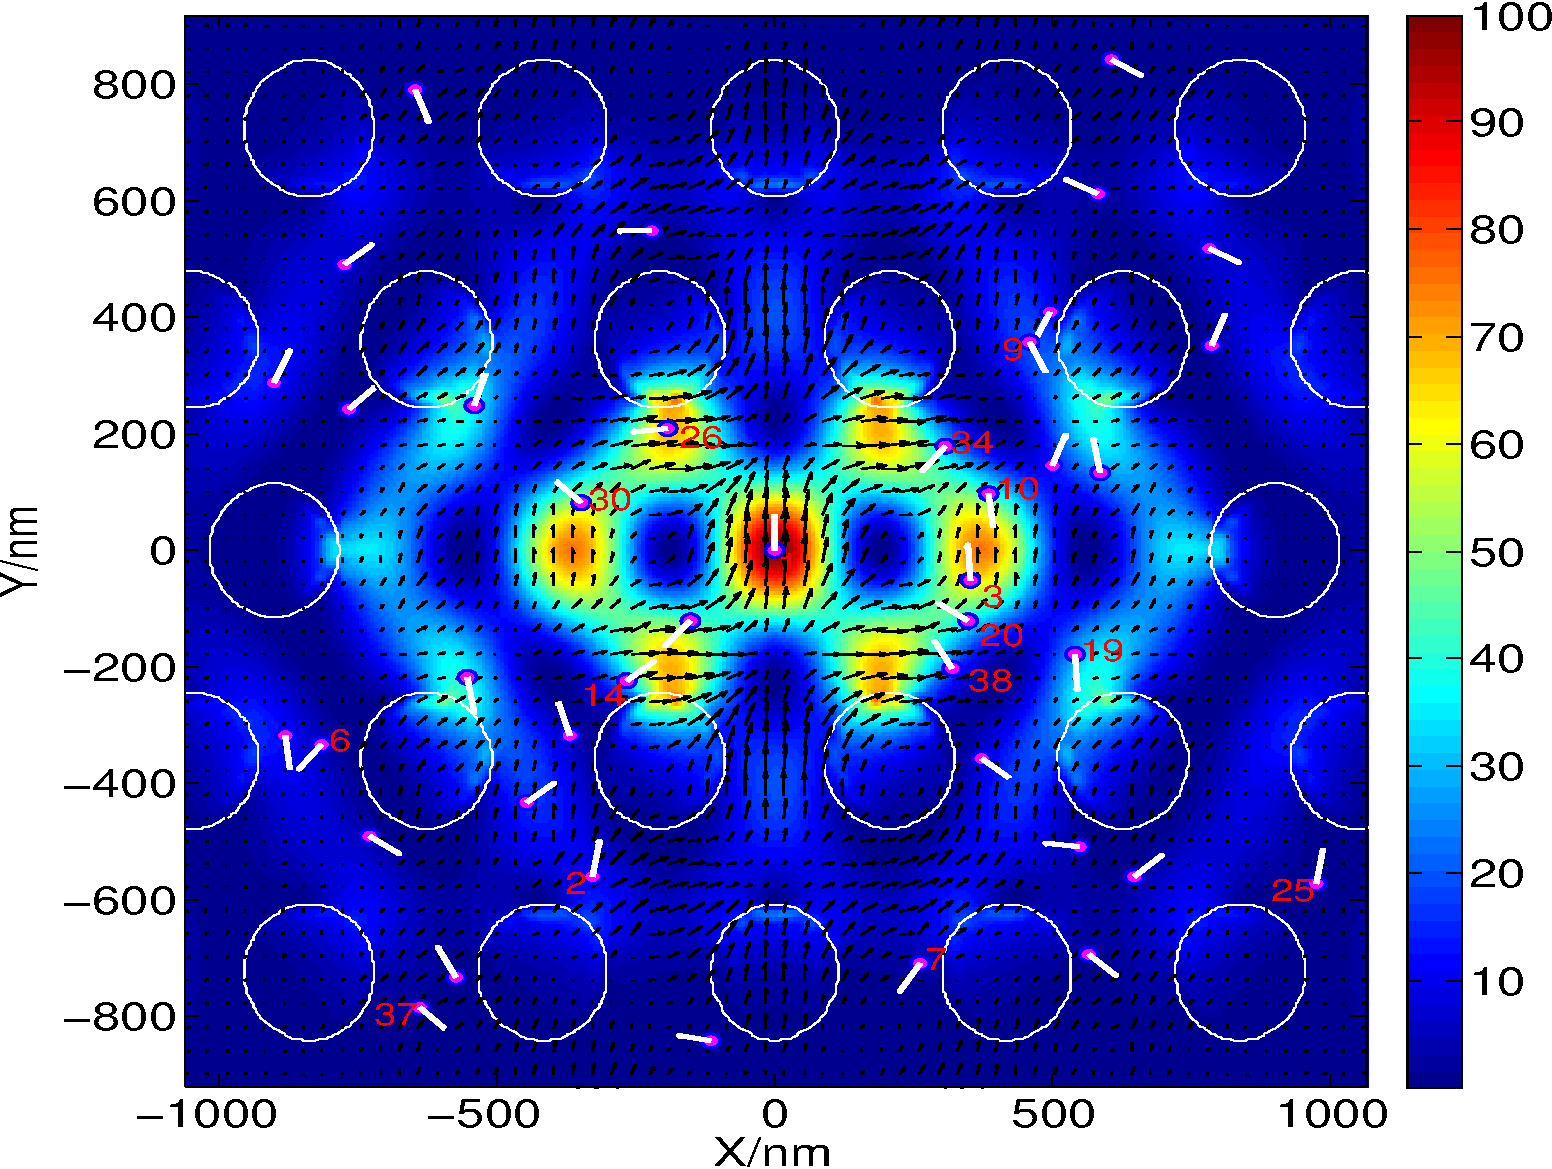
\includegraphics[width=12cm]{./Figs/QDmode}
\end{center}
\caption[Cavity mode and 41-QD distribution in a PC cavity.]{\textbf{  Cavity mode and QDs distributions map.} The background color map shows the electrical field strength, with black arrows indicating the field directions. The pink dots with white tails indicate the position and oscillating directions of the QDs. Numbers nearby the QDs are the labels for interested QDs. }
\label{QDmode}
\end{figure}



\begin{figure}[htp]%[floatfix]
\centering
\begin{center}
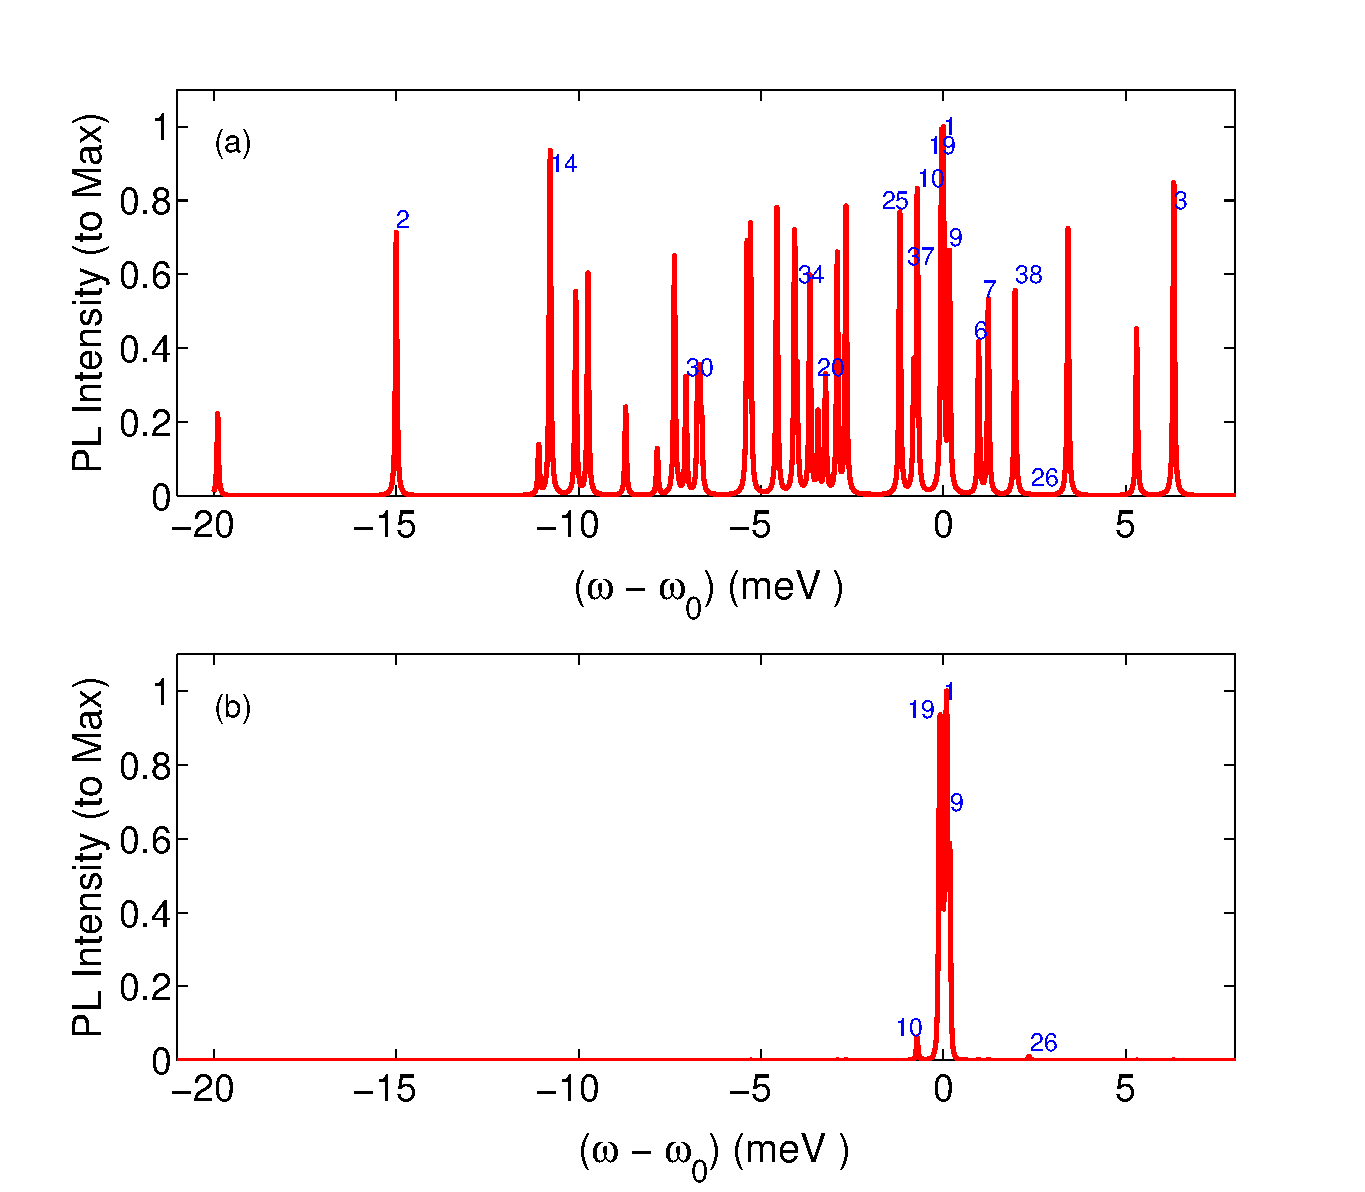
\includegraphics[width=12cm]{./Figs/QDspecPChom}
\end{center}
\caption[Spectra of 41 QDs in a homogeneous medium and a PC cavity.]{\textbf{$Y$-polarized Spectra of 41 QDs in a homogeneous medium (a) and the PC cavity (b).} The QDs ensemble has a Gaussian distribution profile, centered at 5 meV lower than the cavity mode resonance, with standard deviation $\sigma=20$ meV. Numbers around the peaks indicate the corresponding QDs' label. QD 1 is on resonance at $\omega_0$, nearby QDs to the low frequency side are QDs 19 and 10, to the high frequency side are QDs 9 and 26, in the bottom figure.}
\label{QDspecPChom}
\end{figure}

While coupled to the cavity mode, the QD peaks resonating far away from the cavity resonance are washed out, only leaving the cavity peak along with a few QDs peaks either close to the cavity resonance or at strong field positions (see Fig.~\ref{QDspecPChom}(b)).
This result shows that three factors can make the QD peaks visible in a coupled system.
One is the local field strength, and another is the magnitude of dipole moment projected on local field direction.
These two factors, multiplied together, give the coupling strength of the QD to the cavity.
The last factor is the related position of QD's resonance to the cavity resonance.
The closer these two resonances are, the larger the spectral peak occurs.
This factor shows an inhomogeneous enhancement of spectral formation in oscillators coupling.
In sum, the coupling strength and resonance positions will greatly affect the cavity optical property.
%We will discuss the two factors in the following sections.

As we will see, the relative positions of the dipole resonances and the cavity resonance can give various spectral effects, including frequency repulsion, attraction, splitting, screening effects and so on. We would like to give a brief visualization of these effects, as they are the foundation for our discussion on dense-dipole coupled systems. As follows, we will discuss the frequency repulsion, splitting and screening effects by shifting the resonance of the No.1 QD from $+0.6$ meV to $-0.6$ meV around the cavity resonance, while keeping all the other QDs in the PC slab as before. The spectrum is shown in Fig.~\ref{QDwd1shift}.
As we can see, when QD 1 is on the high frequency side of the cavity resonance ($\Omega_1-\omega_0>0$), the observed QD 1 peak (see the wave envelope around the blue dashed line) is on the high frequency side of the intrinsic resonance position where it's supposed to be (marked with blue dashed line in Fig.~\ref{QDwd1shift}). The cavity peaks (two or three peaks very close to the cavity resonance are combined as cavity peaks in this discussion) is enhanced on the far side to $\Omega_1$, while the cavity coupled peaks close to $\Omega_1$ are suppressed. A similar effect occurs when the QD 1 is on the low frequency side of the cavity resonance. The displacements of the dipole and cavity peak show the frequency repulsion effect introduced earlier. If $\Omega_1=\omega_0$, the cavity shows a doublet (here, $g_1>\Gamma_1$), which illustrates the establishment of the strong coupling effect between QD 1 and the cavity and gives the spectral splitting effect. One may have also noticed that there is a small dipole peak (labeled as QD 19, close to the cavity resonance) merging in the cavity peak and basically keeps it stable, regardless of the moving of QD 1 in frequency domain. This stability of the dipole peak in a cavity peak can be called screening effect.

One can find that the closer QD 1 is to the cavity resonance, the larger the repulsion effect becomes (for example, by comparing the QD 1 shifts of the observed peak to its intrinsic resonance between occasions of $\Omega_1=\omega_0+0.6$ meV and $\Omega_1=\omega_0+0.4$ meV). The same applies to the dipole-dipole coupling. If we compare the offset of QD 1 peak to its original resonance at $\Omega_1=\omega_0-0.6$ meV and $\Omega_1=\omega_0+0.6$ meV, we find that the former one is smaller than the latter one, because in the former case, there is a QD 10 coupling to QD 1 as well, which also generates a repulsion effect for the QD 1 peak in the opposite direction to cancel a part of the repulsion effect from the cavity peak. However, the repulsion effect from QD 10 to QD 1 is not strong enough to totally cancel the repulsion from the cavity, as the field strength at QD 10 is much smaller than that at QD 1. The amplitude changes obey the same rule as the shifts. One can find that QD closer to the cavity resonance can give larger influence on the cavity peaks compared to the far-off-resonance cases. In the case of discrete dipoles in coupled cavities, if a dipole is too far away from the cavity resonance (dipoles outside of the calculation range in Fig.~\ref{QDwd1shift}, for example), its influence is negligible. This resonance distance related enhancement effect can be called as inhomogeneous enhancement effect.

%This inhomogeneous enhancement effect will also be discussed for the dense dipoles coupled cavities later.

%The other phenomenon we can see in the process is inhomogeneous enhancement of coupling. We can see that when $\omega_1$ is far off the cavity resonance, the QD 1 peak is relatively smaller than the case when $\omega_1$ is close to the cavity resonance, compared to the maximum value of the spectrum. Compared with the peak height of QD 10 sitting at the position where the cavity peaks raise little effect on it, if we look at the cases when QD 1 is not in the left side of the cavity resonance, we can conclude that the maximum value of the cavity peaks is much larger when QD 1 is close to it than the opposite cases. What's more, the QD 19 and QD 9, which are close to the cavity resonance, can give large peaks even when all other QDs are far away from them. In sum, we can conclude that the near-on-resonance QDs can give larger contribution to the cavity spectrum, and hence can change the cavity's optical property much more than that are far away from the cavity resonance. We will discuss the inhomogeneous broadening effects further in the following sections.

\begin{figure}[htp]%[floatfix]
\centering
%\begin{center}
\subfigure[ ]{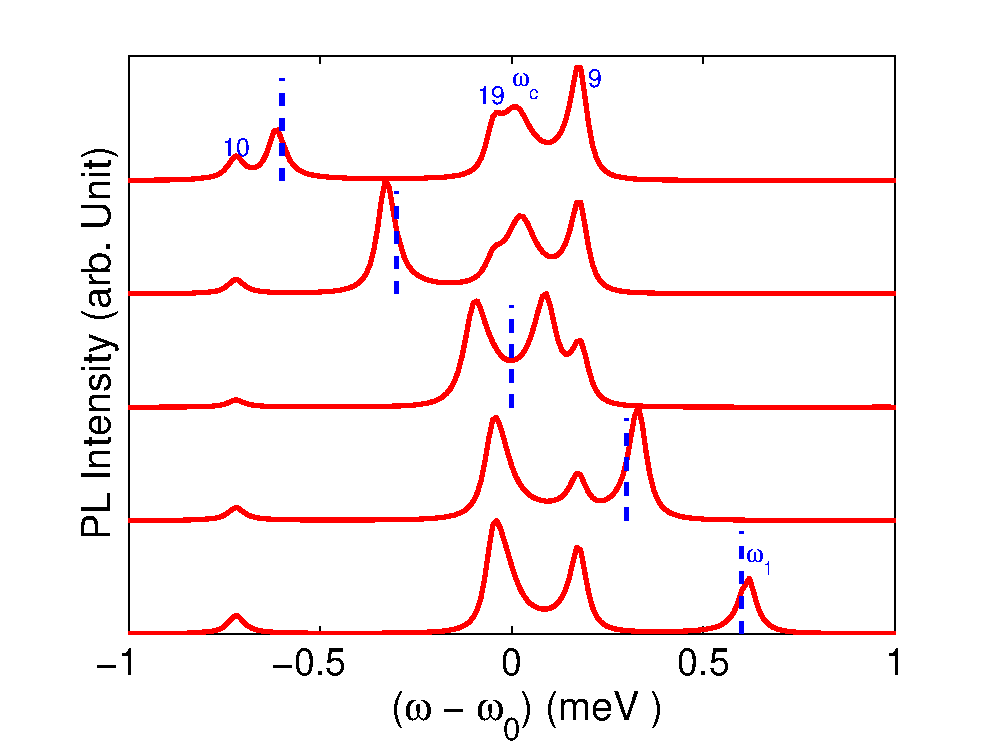
\includegraphics[width=0.46\textwidth]{./Figs/QDwd1shift}
%\end{center}
%\caption{\textbf{Spectrum changes as Dot1 moves around.} The QDs ensemble has a Gaussian distribution profile, centered at 5 meV left to cavity mode resonance, with standard deviation $\sigma=20$ meV. }
  \label{QDwd1shift}}
%\end{figure}
%\begin{figure}[floatfix]
%\centering
%\begin{center}
\subfigure[ ]{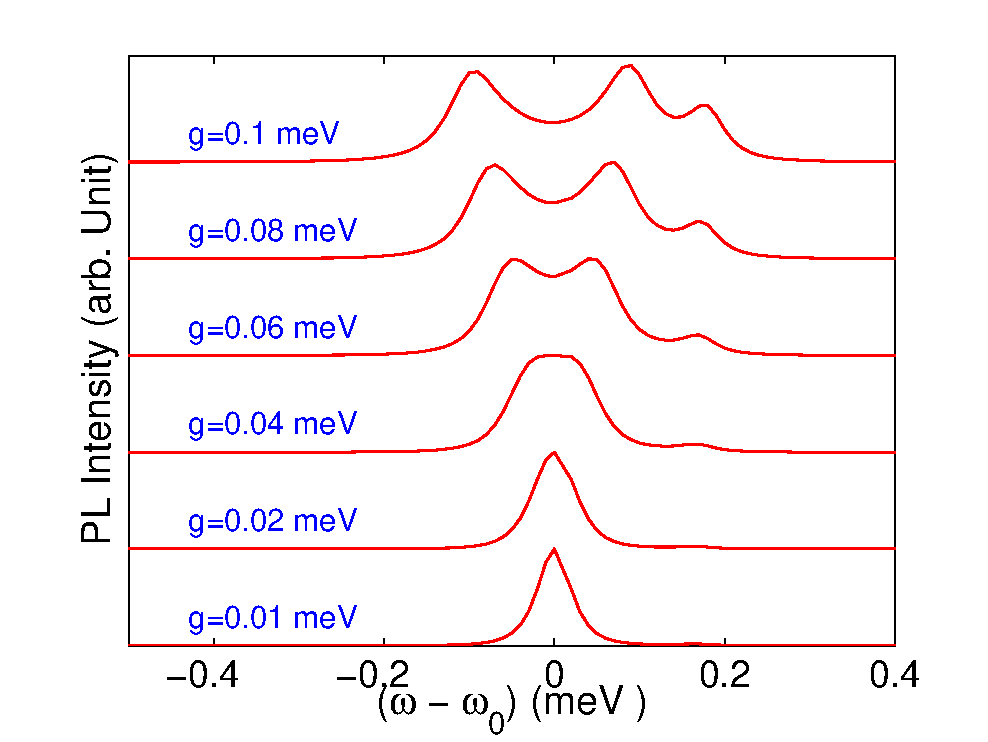
\includegraphics[width=0.46\textwidth]{./Figs/QDdetuneg}
  \label{QDdetuneg}}
%\end{center}
\caption[Cavity Spectra as QD 1 shifts and the coupling constant changes.]{\textbf{Cavity Spectra as the frequency of QD 1 shifts (a) and the coupling constant changes (b).} In \subref{QDwd1shift}, the QD 1 frequency moves from $+0.6$ meV to $-0.6$ meV from bottom to top in steps of $0.3$ meV.
% inhomogeneous coupling and frequency repulsion effects occur (see text). \subref{QDdetuneg} shows, as the coupling strength of QD 1 changes from $0.01$ meV through $0.04$ meV to $0.1$ meV, the cavity shows the Purcell effect, which has a narrower spectrum than $0.1$ meV, and strong coupling effect, which shows a resonances splitting and broadening effects.
 }
\end{figure}

Experimentally, one can tune the resonance of a QD by changing the temperature, and observe the frequency repulsion and inhomogeneous enhancement effects in cavities (see, for example, Refs.~\onlinecite{Reithmaier2004,Reitzenstein2006}). The cavity shifts and enhancement can be easily observed experimentally, since the intrinsic resonance of the cavity is basically static with changing temperature. For the QD's resonance, however, it is only through a careful calculation, as we performed above, can one notice the slight repulsion effect.

To examine how coupling strength matters, one can tune the coupling strength between the QDs and the cavity by changing the optical moments of the dipoles while fixing the QD 1 on-resonance to the cavity. The spectral changes are shown in Fig.~\ref{QDdetuneg}. We can see that the doublet occurs when the critical condition for strong coupling is satisfied, which is $g_1>\frac{1}{2}\Gamma_c=0.05$ meV for the one-exciton case~\cite{Kimble1998}. If $g_1<0.5$ meV, the QD 1 is in a weak coupling regime to the cavity, which means there is a spontaneous enhancement caused by the Purcell effect~\cite{Purcell1946,G'erard1998}. We will discuss this effect in the context of dense dipoles coupled cavities in the next chapter.



%     \begin{Listing}[H]
%     \filein{Examples/List.als}
%     \caption{Alloy specification of a singly-linked list using only binary relations}
%     \label{list:SimpleList1}
%     \end{Listing}
%
%
% \subsection{Phase 1: High-Level Static Mapping}\label{sec:phase1}
%
%     ...Phase 1 simply generates the default static
%     mapping and presents it to the user, as shown in Figure~\vref{fig:defaultMap}.  We
%     have modified the map file as shown in Figure~\vref{fig:fixedMap}.
%
%     \begin{figure}[H]
%     \begin{singlespacing}
%     \centering
%         \subfigure[Default static mapping]{
%             \begin{minipage}{2.25in}\footnotesize
%                 {\texttt{List = List\\
%                 List\$first =
%                 List.first\\
%                 Node = Node\\
%                 Node\$next = Node.next\\
%                 }
%                 }\label{fig:defaultMap}
%             \end{minipage}}
%         \subfigure[Modified static mapping]{
%             \begin{minipage}{2.25in}\footnotesize
%                 {\texttt{List = SimpleList\\
%                 List\$first = SimpleList.first\\
%                 Node = Node\\
%                 Node\$next = Node.next\\
%                 }
%             }\label{fig:fixedMap}
%             \end{minipage}}
%     \caption[Excerpt of high-level static mapping file]{Excerpt of high-level static
%     mapping file before and after modification}
%     \end{singlespacing}
%     \end{figure}
%
%
%
%     Figure~\vref{fig:tree_beforeAndAfter} shows the tree
%     before and after deletion, with correctly implemented code.
%     Figure~\vref{fig:tree_commentedOut_mainBody} shows the tree after deletion of the
%     root, when the \texttt{root = n2} statement is not executed.
%
%     \begin{figure}[H]
%     \centering
%     \mbox{
%         \subfigure[Before deletion]{\includegraphics[scale=0.65]{Figures/correct_pre}}\label{fig:tree_correct_pre}
%         \subfigure[After correct deletion]{\includegraphics[scale=0.65]{Figures/correct_post}}\label{fig:tree_correct_mainBody}
%         }
%     \caption[Visualization of tree]{Visualization of tree before and after correct deletion of the root node}
%     \label{fig:tree_beforeAndAfter}
%     \end{figure}
%
%     \begin{singlespacing}
%     \begin{figure}[H]
%     \centering
%     \includegraphics[scale=0.75]{Figures/commentedOutWithBetterNumber_post}
%     \caption[Visualization of tree after deletion of root (error or omission)]{Visualization of tree
%     after deletion of the root node, with an error of omission in the code.
%     \texttt{Node\_7} represents the temporary node in the \texttt{swapNodes()} method.}
%     \label{fig:tree_commentedOut_mainBody}
%     \end{figure}
%     \end{singlespacing}

%\chapter{Photon Emitters Ensemble and a Cavity Interactions}\label{ch:ensemble}
\chapter[Many-dipole Coupled Cavities]{A large Number of Dipoles Coupled to a Cavity}\label{ch:ensemble}

%\section{A Few Dipoles Coupled Cavity Spectrum}

%\section{A Large Amount of Background Dipoles Coupled Cavity Spectrum}

As discussed in Chapter~\ref{ch:intro}, a good excitons-coupled-cavity model is required to examine the effects of collective emission. A large number of excitons coupled to an optical cavity will be studied in this chapter in the GF method.

This chapter is organized as follows. First, we will define the variables, method and model used for cavities with an arbitrary number of excitons. Next, we will relate macroscopic parameters of pumping rates to the microscopic number of excitons. Then we will show how the collective emission modifies the cavity spectra in several cases.

\section[Model and Method]{Model and Method}\label{Theory}
We will follow the model and calculation method of GFs presented in Chapter~\ref{ch:theory}. Most of our discussion in this chapter falls into the two scenarios introduced in section~\ref{section:scenarios}, in which there are a large number of background dipoles and none or one target dipole in the optical cavity.

%Definition of total spectrum and target spectrum... the total cavity and the target dipole spectra, labeled as $S^{total}$ and $S^{t}$, respectively.
We use the mixed state described in Section~\ref{section:initialcondition} as the initial condition. The total incoherent spectrum for a $N$-dipole coupled cavity, or total cavity spectrum, is given by Equ.\eqref{eq:sN_mixedstate_withdecay}. We represent it here:
\begin{equation}
\mathbf{S}^{total}(\br,\omega)\approx \frac{1}{N\varepsilon_0^2}\sum_{i=1}^N{\left| \mathbf{G}^{(N)}(\br,\br_i,\omega)\cdot {\bm \mu}_i(\omega) \right|^2 \frac{1}{|\omega-\Omega_i+i\Gamma_i/2|^2}}. \label{spectrum}
\end{equation}
%\begin{equation}
% \label{spectrum}
% \mathbf{S}^{total}(\br,\omega)
% %=\left|\mathbf{E}^{(N)}_c(\br,\omega)\right|^2+\left|\mathbf{E}^{(N)}_s(\br,\omega)\right|^2 %,
%\end{equation}
%where
%\begin{align}
% \mathbf{E}^{(N)}_c(\br,\omega) &=\langle \E0\nonumber\\
%~~&+\sum_n{\GN_{\rrn}\cdot \Alphanw \cdot \Enw0}\rangle,\\
% \mathbf{E}^{(N)}_s(\br,\omega) &=\langle \sum_n{\GN_{\rrn}\cdot \dnw}\rangle %\label{Esource}
%\end{align}
%are the cavity and source fields considering the $N$ dipoles.
%
And the spectrum from the target dipole is given by
\begin{equation}
 \label{spectrum}
 \mathbf{S}^{t}(\br,\omega)=\left|\langle \GN_{\mathbf{r},\mathbf{r}_t}\cdot \hat{\mathbf{d}}_t(\omega)\rangle\right|^2 = \frac{1}{N\varepsilon_0^2}
 {\left| \mathbf{G}^{(N)}(\br,\br_t,\omega)\cdot {\bm \mu}_t(\omega) \right|^2 \frac{1}{|\omega-\Omega_t+i\Gamma_t/2|^2}}.
\end{equation}
The superscript ``$t$'' denotes the target dipole which usually has a relatively large coupling strength to the cavity.

Generally, when two resonators couple together, two effects dominate the change of the spectra shapes: one is the frequency repulsion effect, in which two distant spectral peaks repel each other; the other is the direct broadening effect, in which a small spectral peak is merged into another peak and broadens the second peak. Also when a repulsion happens, the inner half of a peak is usually shifted much faster than the outer half of the peak, which results in a narrowing effect on the spectral peaks. We have discussed these two effects in section~\ref{PCcase}. This chapter will show that these two effects give rich behaviors of the ensemble spectrum.

%I have divided the effects which broadens the spectrum into two orders: the first-order broadening effect comes from the background dipoles imposed to the original spectrum; the second-order effect comes from the inhomogeneous repulsion applied from the neighboring background dipoles, in which the repulsed shift of the nearside leaf of the spectrum is always larger than that of the farside leaf. When there are much more dipoles on one side of the spectrum, the second-order broadening effect may overtake the first-order effect and gives a narrower spectrum.


% phase changing effect

%\begin{figure}[floatfix]
%\centering
% \begin{tabular}{cc}
%   \subfigure[ Dipoles distribution.]{\label{distr_wd0.5s0.1}
    %\psfrag{x}{$\omega-\omega_c$ meV}
    %\psfrag{y}[][]{Number of Dipoles}
%    \includegraphics[width=0.23\textwidth,height=0.21\textwidth]{./Figs/distr_wd0.5s0.1}}
%  &
%    \begin{minipage}[t]{0.49\linewidth}
%    \centering
%    \subfigure[ FWHM of cavity peak. ]{\includegraphics[width=1\textwidth,height=0.93\textwidth]{./Figs/FWHMcav_2000wd0.5s0.1}
    %\caption{\textbf{FWHM of cavity peak.} The QDs ensemble has a Gaussian distribution profile, centered at $-0.5$ meV left to cavity mode resonance, with standard deviation $\sigma=0,\,0.05,\,0.1$ meV. }
%    \label{FWHMcav_2000wd0.5s0.1}}
%  \end{minipage}
% \end{tabular}
%\caption{\textbf{Off-resonance ensembles coupled cavity system.} \subref{distr_wd0.5s0.1} gives an example of the gaussian distribution profile of 2000 background dipoles' resonances, with $\sigma=0.1$ meV and $\Delta\omega=-0.5$ meV. \subref{FWHMcav_2000wd0.5s0.1} shows the cavity width is changing as a function of $N$. The inset shows the oscillation feature of bandwidth changing. The curve is averaged from $200$ samples of $\sigma=0.1$ meV dipoles sets.}
%\end{figure}





%\clearpage
\section[Pumping Effect]{Pumping as a Booster for Excitations}\label{PumpingComparison}
As is well known, the spectrum of cavity systems can be reshaped under pumping; however, the mechanism is still in debate. In this section, we show that, in the linear region, pumping is actually equivalent to exciting background dipoles.

In some cases, it has been shown that the few-dipole approximation holds to fit the spectrum of a cavity with many excitons~\cite{yao2010nonlinear,Reitzenstein2010}. Moreover, in the ME models with the one- or few-exciton approximation, the pumping effect can be characterized by the pumping rate, $P=P_c+P_x$, where $P_c$ is the cavity pumping rate and $P_x$ is the exciton pumping rate~\cite{yao2010nonlinear}. The total pumping rate, $P$, is shown to be proportional to the pump power, by fitting the experimental spectral data with the ME models.

By numerically fitting our GF model of the $N$-dipole cavity system to the spectrum predicted by a one-exciton ME model, we find that the GF and ME models are consistent with one another. The curves of fitted spectra and pumping rates, based on a least square method (LSM), are shown in Fig.~\ref{fig:GFT_ME_fits}. We use the following master equation for our ME model as suggested in Ref.~\onlinecite{yao2010nonlinear} with both cavity and exciton baths included:
\begin{equation}
\begin{split}
  \dt \rho & = \frac{1}{i\hbar}[H_s,\rho] + \frac{\Gamma_c+P_c}{2}(2a\rho\adag - \adag a\rho - \rho\adag a)\\
& +\frac{\Gamma_x+P_x}{2}(2\sigm\rho\sigp - \sigp\sigm\rho - \rho\sigp\sigm ) \\
& +\frac{P_c}{2}(2\adag\rho a - a \adag\rho - \rho a\adag) \\
&+ \frac{P_x}{2} (2\sigp\rho\sigm - \sigm\sigp\rho - \rho\sigm\sigp )\\
&+\frac{\Gamma_x^{\prime}}{4} (\sigz\rho\sigz-\rho),
 \end{split}
\end{equation}
where the intrinsic Hamiltonian of the exciton-photon system can be given under the rotating wave approximation~\cite{Gerry2005} by
\begin{equation}
 H_s=\hbar\omega_c \adag a+ \hbar \Omega_x \sigp\sigm +\hbar g(\sigm \adag+\sigp a).
\end{equation}
Here, $a$ and $\adag$ correspond to the annihilations and creation operators of photons. $\sigma^-$ and $\sigma^+$ correspond to the annihilations and creation operators of excitons. $\rho$ is the density operator. $\Gamma_c=g=0.1$ meV. $\omega_c=\omega_0$ and $\Omega_x$ are the cavity and exciton resonances. The spectra we calculated is for a continuously pumped cavity. For the GF model, we have assumed there is a target dipole corresponding to the exciton at $\Omega_x$ in the ME model, and there are a large number of weakly coupled background dipoles with a Gaussian distributed profile with a wide standard deviation, $\sigma=20$ meV), and $\Delta\omega=\Omega_d-\omega_0=0$, $g_b=0.02$ meV. All other GF parameters are consistent with the ME model. The GF spectra are averaged over $400$ sets of samples to reflect the statistic nature of the ME model, each with up to $1000$ background dipoles, to give a smooth spectrum for both the target dipole on-resonance and off-resonance ($\Omega_t=\omega_0-1.0$ meV) cases as shown in Figs.~\ref{fig:GFT_ME_fits} (a) and (c), respectively.


\begin{figure}[htp]%[floatfix]
     \centering
     \subfigure[ ]{
          \label{fig:GFT_ME_spec_str}
                %\psfrag{ylabel}{$\frac{1}{\sigma}\frac{\rmd\sigma}{\rmd\ptsq}\gev^2$}
                %\psfrag{xlabel}{\small{$\ptsq\gev^2$}}
          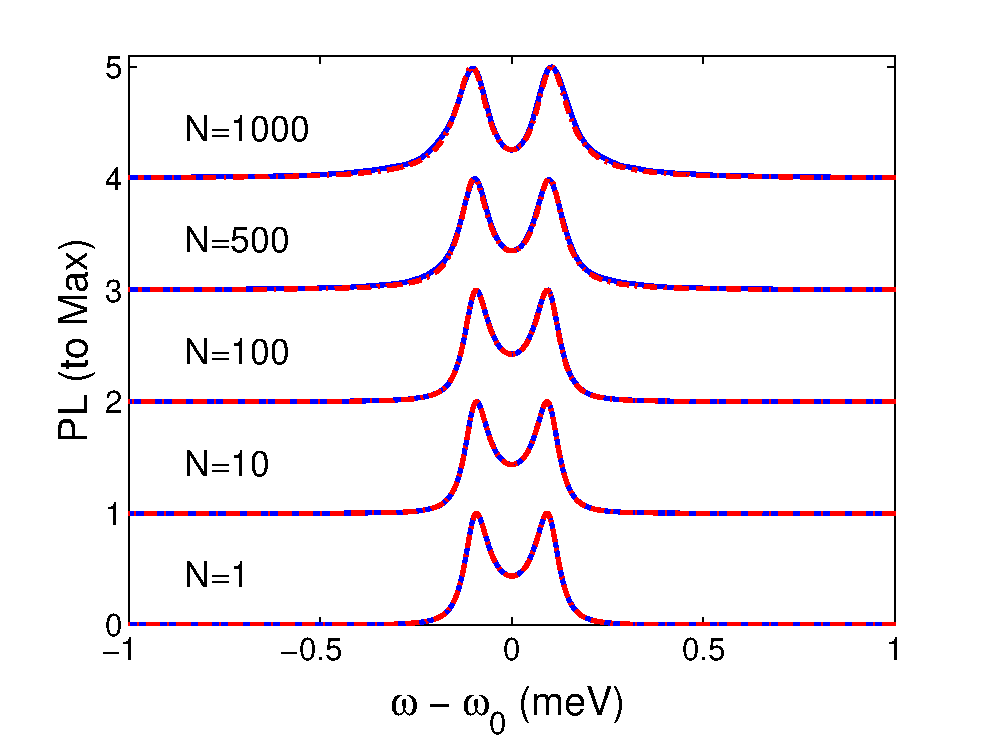
\includegraphics[width=.46\textwidth]{./Figs/GFT_ME_spec_str}}
     %\hspace{.1in}
     \subfigure[ ]{
          \label{fig:P_str}
                %\psfrag{ylabel}{$\frac{1}{\sigma}\frac{\rmd\sigma}{\rmd\ptsq}\gev^2$}
                %\psfrag{xlabel}{\small{$\ptsq\gev^2$}}
          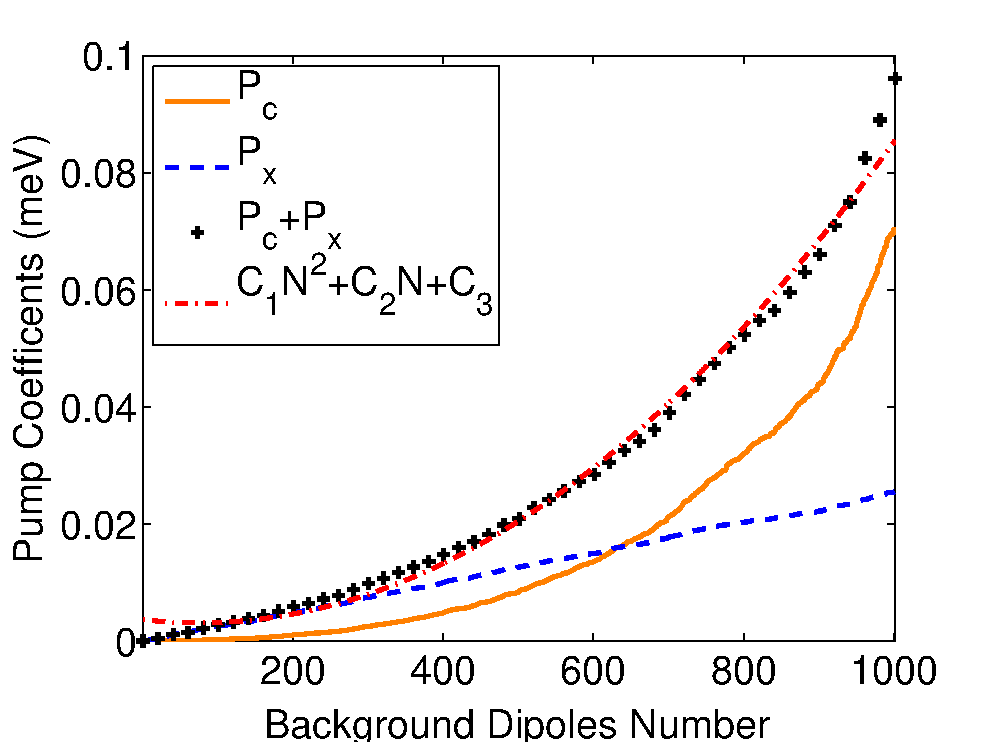
\includegraphics[width=.46\textwidth]{./Figs/P_str}}\\
     %\vspace{.1in}
%     \hspace{.1in}
     \subfigure[ ]{
           \label{fig:GFT_ME_spec_weak}
                %\psfrag{ylabel}{$\frac{1}{\sigma}\frac{\rmd\sigma}{\rmd\ptsq}\gev^2$}
                %\psfrag{xlabel}{\small{$\ptsq\gev^2$}}
           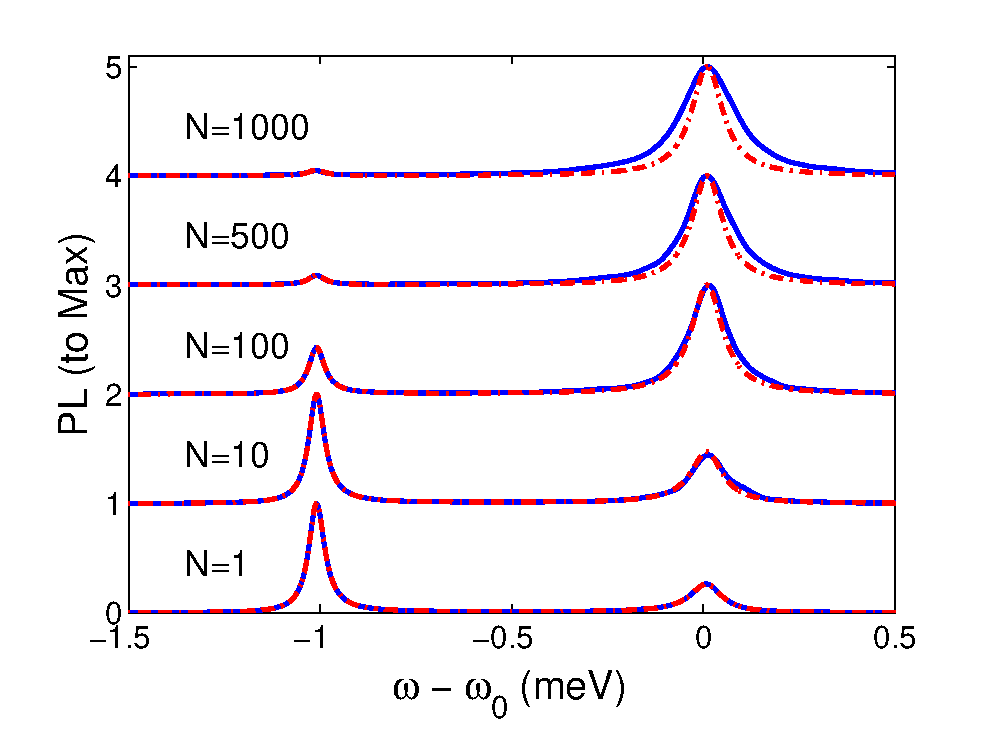
\includegraphics[width=.46\textwidth]
                {./Figs/GFT_ME_spec_weak}}
     \subfigure[ ]{
           \label{fig:P_weak}
                %\psfrag{ylabel}{$\frac{1}{\sigma}\frac{\rmd\sigma}{\rmd\ptsq}\gev^2$}
                %\psfrag{xlabel}{\small{$\ptsq\gev^2$}}
          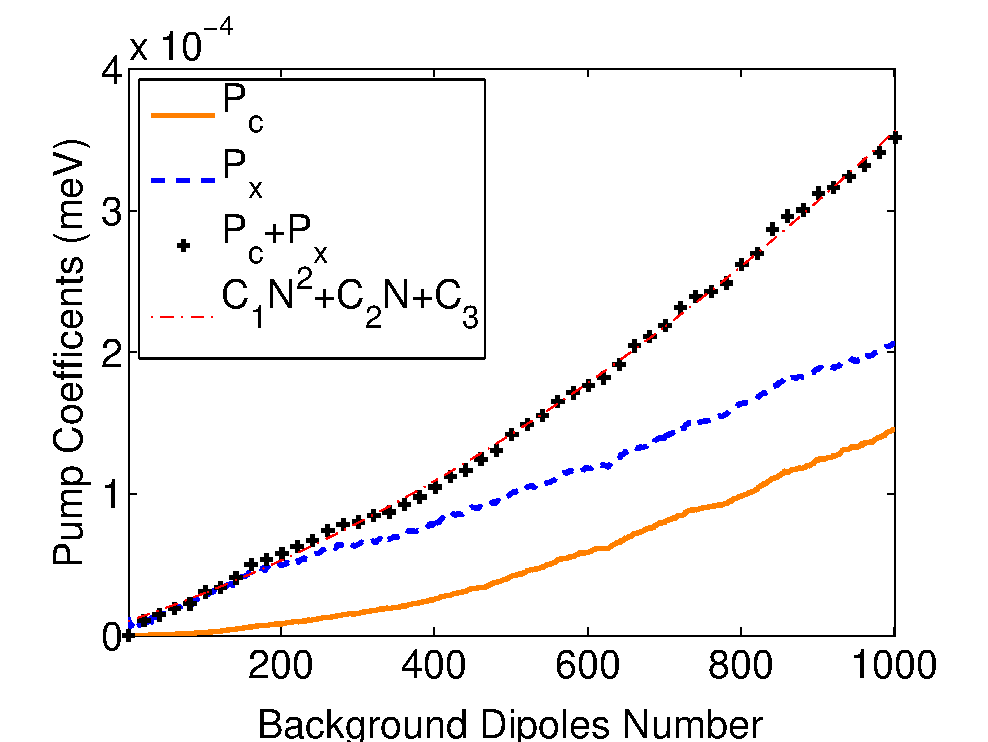
\includegraphics[width=.46\textwidth]{./Figs/P_weak}}
     \caption[Pumping as a tool for dipoles excitation.]{\textbf{  LS fit of ME model to GFT spectra as background dipoles number $N$ varies from $0$ to $1000$.} Both target dipole on-resonance (\subref{fig:GFT_ME_spec_str} and \subref{fig:P_str}) and off-resonance (\subref{fig:GFT_ME_spec_weak} and \subref{fig:P_weak}) cases are calculated. The GFT spectra (solid-blue curves in (a) and (c)) are averages of $400$ samples, each of which has up to $1000$ background dipoles Gaussianly distributed around the cavity resonance with a standard deviation of $\sigma=20$ meV. The best fit ME pumping coefficients $P_c+P_x$ show a good function form of $C_1N^2+C_2N+C_3$. See text for the detailed curve fitting procedure.}
     \label{fig:GFT_ME_fits}
\end{figure}

The curve fitting is performed as follows. First, we calculate the cavity spectra with $N$ dipoles ($N=1,2,\cdots,1000,\cdots$) based on the GF method with the parameters introduced in the last paragraph. Because the background dipoles are randomly distributed, and the spectrum relies on the resonance positions of the background dipoles, to obtain a robust statistical spectrum curve, we have averaged $400$ samples for each specific $N$. Next, we fit the exciton pumping parameter, $P_x$, to the $N=1$ spectrum of the GF method, by using the LSM with the ME spectrum formula (Equ.\eqref{S_ME}) with $P_c=0$. We can get a perfect fitting since the GF spectrum of $N=1$ is equivalent to the ME model described above with sole exciton pump (the target dipole is excited without any pump to the cavity mode)~\cite{Hughes2009}. Then, we use the best fitted $P_x$ and $P_c=0$ obtained above when $N=1$ as the initial values, and fit the next best pumping rates, $P_x$ and $P_c$, of the ME model to the GF spectrum of $N=2$, by using the LSM. We increase the $N$ one by one, and repeat the step above until $N$ is large enough. One may need to carefully adjust the iterative steps and tolerance of errors in the LSM setting to find the smoothly increasing pumping parameters of the ME model as $N$ increases. Our results are shown in Fig.~\ref{fig:GFT_ME_fits}.

We find that the two models fit very well in the linear region, and the pumping rates are correlated with the number of background dipoles with a clear physical meaning. As plotted in Figs.~\ref{fig:P_str} and~\ref{fig:P_weak}, for both on-resonance and off-resonance coupling cases, the pumping rate $P$ fits well a second order polynomial functions of $N$, which is $P=C_1N^2+C_2N+C_3$, where $C_1>0$, $C_2$ and $C_3$ are all constants. The exciton and cavity pumping rates, $P_x$ and $P_c$, are first-order and second-order functions of $N$, respectively. This fact can be interpreted as some excitations under pumping in cavities with homogeneously distributed photon emitters. If we suppose the average distance between photon emitters is given by $L=1/n$, where $n$ is the line density of emitters, and $\mathcal{S}$ is the luminescent area where there are $n^2$ excitons per unit area, then there are two interpretations of the second-order polynomial correlation relationship between pumping rates and background dipoles numbers: one is that, as the pumping power increases, the mean separation of excitons is not changed, but the luminescent area is enlarged linearly; the other interpretation is that, as the pumping power increases, the luminescent area is not changed, but the mean distance between excitons decreases linearly, or the number of excitons per unit area increases. The former interpretation may correspond to a large cavity with a limited or inhomogeneous pumping area, such as laser pumped molecular luminescence in a solution cavity; the latter one may correspond to a large pumping area with a limited cavity volume, such as optical pumped micropillar QDs single photon sources, where every QD could excite several excitons as pumping power is increased. Experimentally, it is possible to estimate how many color centers are excited in a microdisk cavity based on the scanning confocal image~\cite{Santori2010}, and the changing of the population of luminescent spots is consistent with the interpretations. Correspondingly, $P_c$ and $P_x$ both depend on the increasing number of excited dipoles coupled to the cavity, as both parameters are functions of $N$. All of the coupling between the background dipoles and the cavity are through the target dipole which has a stronger coupling strength to the cavity, since the the fitted parameters of $N$ depend on the relative position of the target dipole.

Notice that, since the number of physical luminescence centers, such as QDs in a semiconductor laser cavity or ions in a large liquid cavity, may not equal the actual number of excitons; the $N$ which we use throughout this paper refers to the number of excited excitons or dipoles. The cases of increasing $N$ can be realized by increasing the pump power or physically increasing the number of luminescent centers in all ways.

Although the two models fit well at first glance, the ME model in the one-exciton approximation fails to describe the inhomogenous broadening effect caused by the background dipoles (see the mismatch of the cavity spectra with $N>500$ in Fig.~\ref{fig:GFT_ME_spec_weak}). As the GF theory shows, depending on the distribution profile of the background dipoles, the spectrum of the ensemble coupled cavity can be reshaped into a non-Lorentzian envelope. The ME model fails in this case, because it cannot reflect the non-Lorentzian distribution of background dipoles.





\section{Cavity spectral behavior with an ensemble of background dipoles}

%As we discussed before, the ensemble of background dipoles can be treated as an entity, basically. So, the relative central resonance and effective optical moment (determined by the dipoles population) of the background dipoles will strongly affect the optical property. And a simplified few-dipole model can be used to analyze the cavity spectrum.


In section~\ref{PCcase}, we looked at the spectral behavior of a PC cavity with numbered background dipoles and one target dipole, and introduced some basic effects of changing the properties of optical cavities. In this section, we will move on to the discussion of dense dipoles coupled cavities. All results in this section are calculated using the GF method.



%\section{Spectral Behavior for Dense-dipole Coupled Cavities}\label{Onedipolecoupling}
%In this section, we will discuss a large amount of background dipoles coupled cavities.
Based on GF calculations, we find that, when all dipoles are far off the cavity resonance, the Purcell effect occurs and the cavity peak is repelled and narrowed. If there are some dipoles merged into the cavity peak, however, the cavity spectrum will be broadened and shifted, and the shift of the cavity peak center is affected by both the nearby and far-off-resonance dipoles in a complicated way. We discuss these two cases in detail.

\subsection{Cavities with Far-off-resonance Dipoles}
To show how far-off-resonance dipoles affect the cavity spectrum, we consider in a homogeneous field up-to $2000$ background dipoles which have an equal coupling strength and are off the cavity resonance. The same dipoles and cavity parameters as that of the last section are used, except for the dipole resonances. One example of the distribution of $2000$ dipole resonances is shown in Fig.~\ref{distr_wd0.5s0.1}. Now, let us increase the number of background dipoles from $1$ to $2000$, and average $200$ samples to get the mean values for the cavity shifts and widths as functions of dipole population. The cavity peak shift and the peak frequency of the dipoles ensemble shift are shown in Fig.~\ref{peakshift_wd0.5_detune_N}. Both exciton and cavity peaks are repelled from the center of the original $\Omega_d$ and $\omega_0$. The spectral shift is proportional to the effective coupling strength or $\sqrt{N}g_b$~\cite{Kimble1994}. The FWHM of the cavity spectrum is shown in Fig.~\ref{FWHMcav_2000wd0.5s0.1}. Note that the cavity spectrum will be narrowed down towards the individual dipole decay rate, which is consistent with the Purcell effect. In our case, when all dipoles are far off the cavity resonance, the photon is scattered among the background dipoles, and the decay time is increased, and hence the FWHM of the cavity spectrum is narrowed down. Moreover, both the cavity spectral shift and bandwidth curve match up the cases with defined dipoles when all dipoles share the same resonance and when there is only one dipole coupled to the cavity with a growing coupling strength. As has been discussed in Section~\ref{section:scenarios}, once the background dipoles have close resonances, the dipole ensemble is equivalent to a single effective dipole with a larger coupling strength of $\sqrt{N}g_b$ to the cavity.


\begin{figure}[htp]%[floatfix]
\centering
 \begin{tabular}{cc}
   \begin{minipage}[t]{0.44\linewidth}
   %\centering
    \subfigure[Dipole distribution with $\sigma=0.1$ meV and $\Delta\omega=-0.5$ meV.]{\label{distr_wd0.5s0.1}
    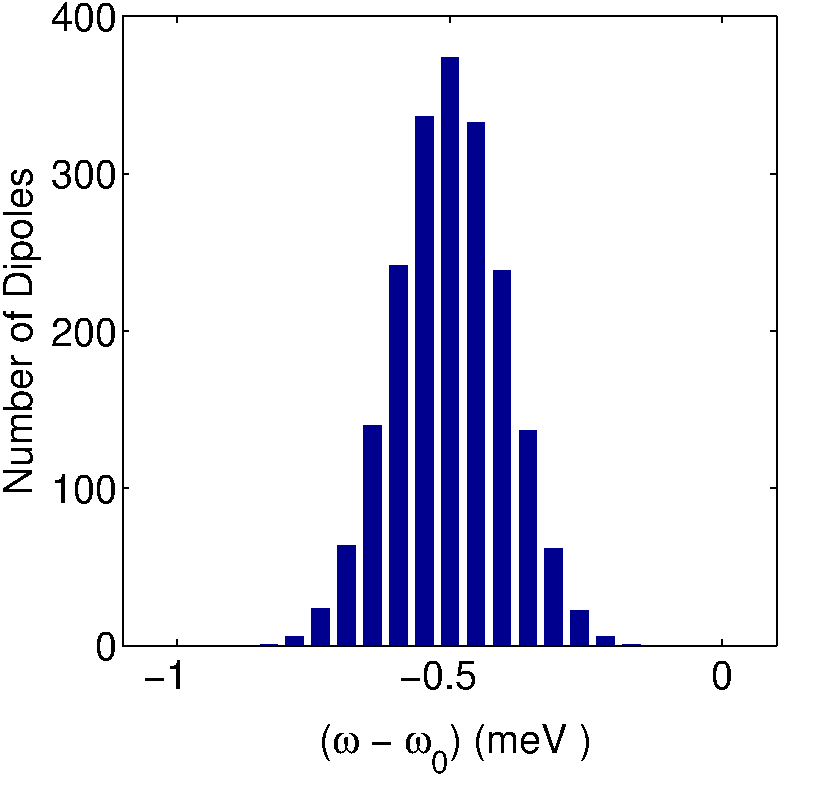
\includegraphics[width=1\textwidth,height=0.9\textwidth]{./Figs/distr_wd0dot5s0dot1}}
   \end{minipage} \qquad
   \begin{minipage}[t]{0.46\linewidth}
   \subfigure[FWHM of cavity peak as a function of $N$. ]{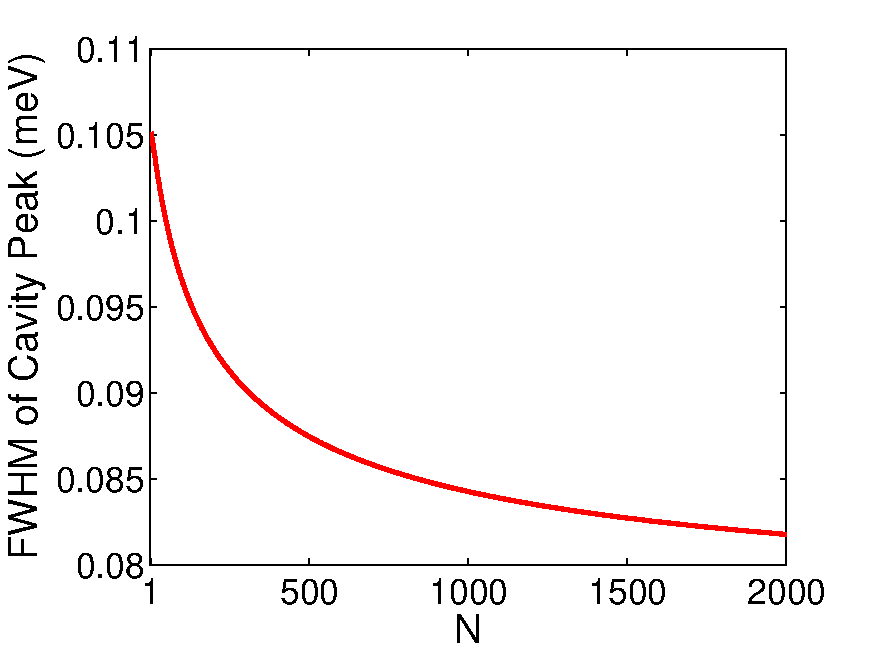
\includegraphics[width=1\textwidth,height=0.9\textwidth]{./Figs/FWHMcav_2000wd0dot5s0dot1}
    %\caption{\textbf{FWHM of cavity peak.} The QDs ensemble has a Gaussian distribution profile, centered at $-0.5$ meV left to cavity mode resonance, with standard deviation $\sigma=0,\,0.05,\,0.1$ meV. }
    \label{FWHMcav_2000wd0.5s0.1}}
   \end{minipage}
   \\
   %\begin{tabular}{cc}
   %\begin{minipage}[t]{0.34\linewidth}
   %\centering
   %\end{minipage}
  %&
  %\begin{minipage}
   \subfigure[Cavity and dipole peak shifts. ]{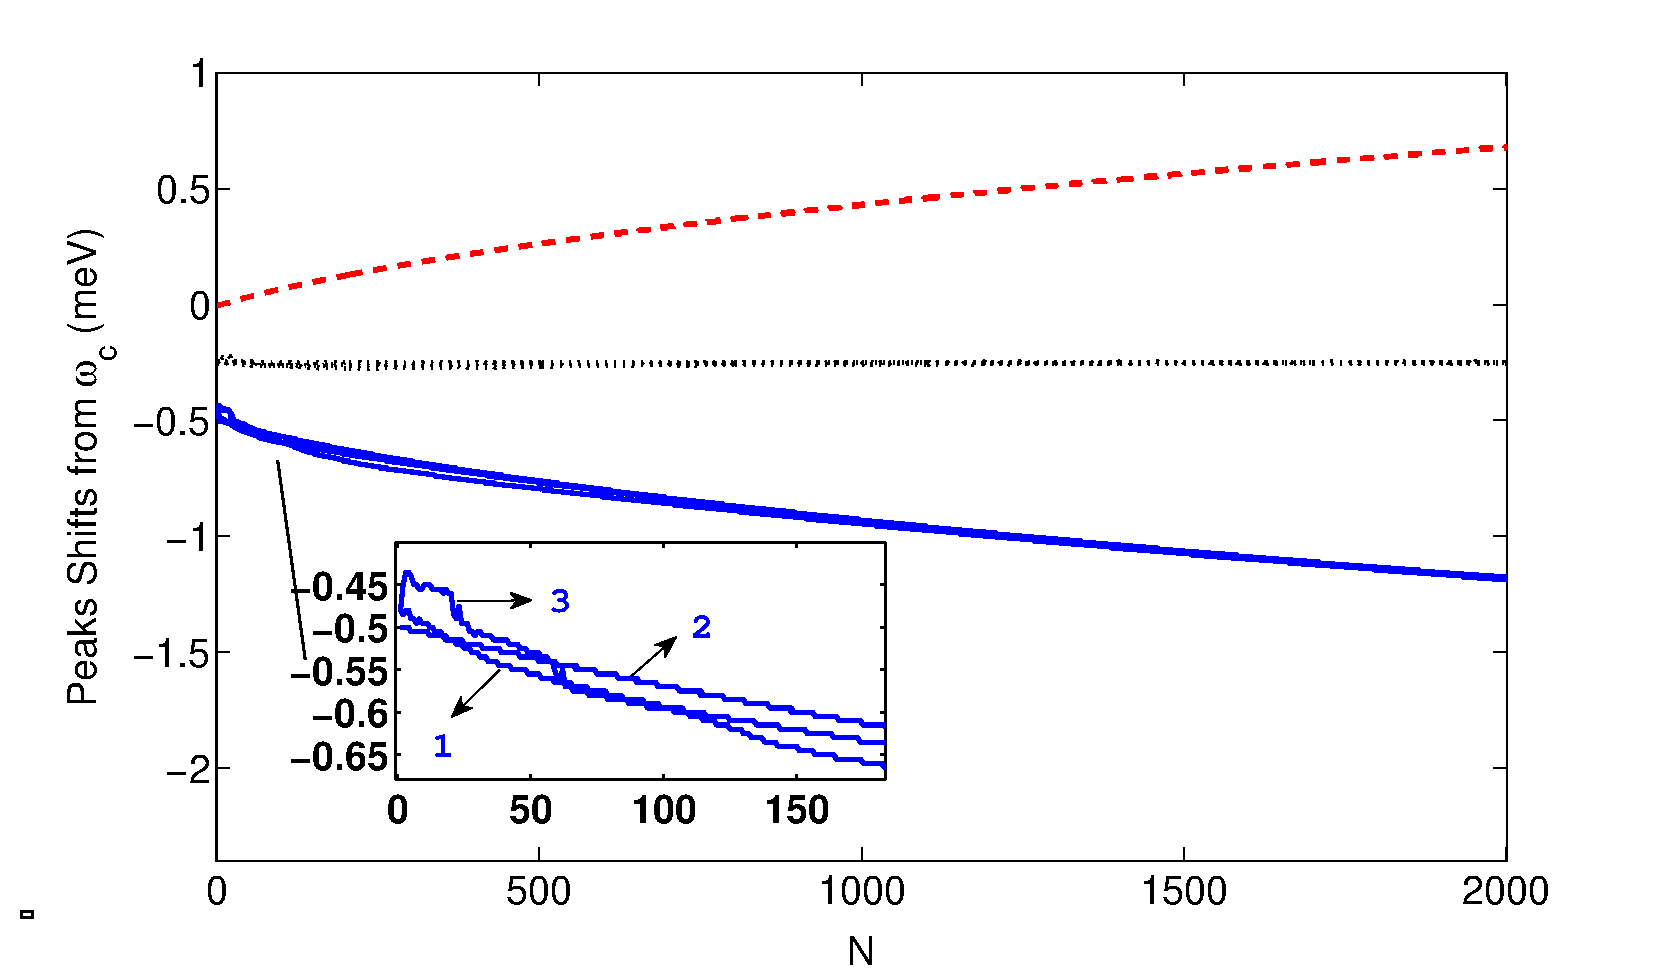
\includegraphics[width=0.56\textwidth,height=0.4\textwidth]{./Figs/peakshift_wd0dot5_detune_N}
    \psfrag{N}{Number of Dipoles}
   %\caption{\textbf{Repulsion effect.} The QDs ensemble has a Gaussian distribution profile, centered at $-0.5$ meV left to cavity mode resonance, with standard deviation $\sigma=0,\,0.05,\,0.1$ meV. }
   \label{peakshift_wd0.5_detune_N}}
  %\end{tabular}
  %\end{minipage}
  \subfigure[Dipole distribution with $\sigma=20$ meV and $\Delta\omega=-5$ meV.]{\label{wddistr_wdrand5s20_qd2000_stat100_2}
    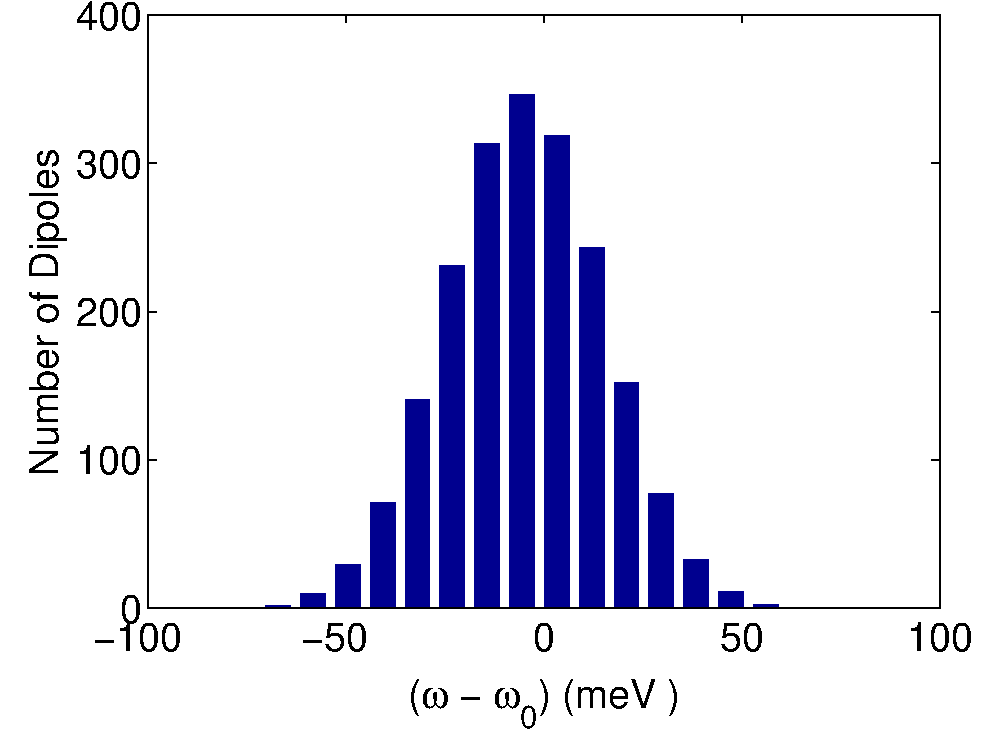
\includegraphics[width=0.40\textwidth,height=0.4\textwidth]
    {./Figs/wddistr_wdrand5s20_qd2000_stat200}}
  %&
  %\begin{minipage}[t]{0.49\linewidth}
  %\centering
  %  \subfigure[ ]{\includegraphics[width=1\textwidth,height=0.9\textwidth]{./Figs/PhaseChange_1wd0.5g0.02}
  %  \label{PhaseChange_1wd0.5g0.02}}
  %\end{minipage}
 \end{tabular}
\caption[Spectral modification of off-resonance ensemble.]{\textbf{  Off-resonance ensemble coupled cavity system.} \subref{distr_wd0.5s0.1} and~\subref{wddistr_wdrand5s20_qd2000_stat100_2} give two examples of the Gaussian distribution profile of dipole resonances with $\sigma=0.1$ meV and $\Delta\omega=-0.5$ meV, and $\sigma=20$ meV and $\Delta\omega=-5$ meV, respectively.
\subref{FWHMcav_2000wd0.5s0.1} shows the cavity width as a function of $N$.
The curve is averaged over $200$ samples of $\sigma=0.1$ meV dipoles sets.
\subref{peakshift_wd0.5_detune_N} shows that both the cavity (dashed red line) and dipoles (solid blue line) peak mean positions change as dipoles number $N$ increases. Inset is a magnified segment of dipole peak position,
where label 1 corresponds to the single-dipole case and equivalent to the $\sigma=0$ case,
label 2 shows the $\sigma=0.05$ meV case,
and label 3 shows the $\sigma=0.1$ meV case.
The difference between the curves is small.}
%\subref{PhaseChange_1wd0.5g0.02} the phase diagram of GF of a single-dipole coupled cavity system with $\Omega_d=\omega_0-0.5$ meV, and $g=0.02$ meV. }
\end{figure}

% phase changing
%Notice that there are some beats in the FWHM changing with respect to the number of dipoles (inset of Fig.~\ref{FWHMcav_2000wd0.5s0.1}). This can be explained by analogically introducing the concept of phase angle, $\theta$, which is commonly used in RLC circuit signal analysis to describe wave beating.

%For a RLC circuit, the tangent of a phase angle is defined by $\tan\theta=\frac{L-C}{R}$ and indicates the power fluctuation caused by phase difference between the current and the voltage~\cite{Neamen2001}, where $L$ is the inductance of the load, $C$ is the capacitance, and $R$ is the resistance of a circuit. Researchers have shown that some cases of dipole-cavity interactions can be equivalent to some simple RLC circuits~\cite{Greffet2010}. And the far-off-resonance case we are discussing is basically a one-dipole coupled cavity system, which has an equivalent RLC circuit. Therefore, we can similarly bring the signal analysis method into our ensemble-cavity coupled system by identifying corresponding quantities of resistance, inductance and capacitance of the equivalent RLC circuits for our case. Following the equivalent circuits method discussed in Ref.~\onlinecite{Greffet2010}, for ensemble coupled cavities, one can analogically define the phase angle as the ratio of the imaginary part and the real part of the field strength that determines the spectrum.
%The only difference between optical system and electronic circuits is that the phase angle becomes a tensor for various optical components.
%For instance, in a single-dipole coupled system, we can obtain the $ij$-component of corresponding phase angle tensor by
%\begin{equation}
%\label{phase}
%\begin{split}
%\tan\theta_{ij} =& \frac{imag(E_i(\br))}{real(E_j(\br))}\\
%=& \frac{-\omega\left[\Gamma_d (\omega^2-\Omega_d^2)+\Gamma_i (\omega^2-\Omega_d^2)\right]}{(\omega^2-\omega_j^2) (\omega^2-\Omega_d^2)-\omega^2 \Gamma_j \Gamma_d-4g^2 \omega_j \omega},
%\end{split}
%\end{equation}
%where $i,j=x,y,z$ label different mode components of the cavity, $\omega_j$ indicates the $j$-th mode in orthogonal directions, and $\Omega_d$ and $\Gamma_d$ are the resonance and decay rate of the dipole. For single-direction polarized cases with single cavity mode, the phase angle tensor is reduced to a scalar ($i=j$). In Fig.~\ref{PhaseChange_1wd0.5g0.02} for a given $g$, we can see that at exciton and cavity resonances, the phase approaches to $\pm \pi/2$, which means the electrical field has almost only the imaginary part; while at frequencies far away from resonances, the phase angle approaches to $0$, which corresponds to a pure real electrical field. Generally, the imaginary part of the field usually has a Lorentzian lineshape, and the mode of the real part of the field is basically outside of the imaginary part. Recalling that the phase angle determines the relative magnitude of the real and imaginary parts, therefore, the tangent of the phase angle can reflect the linewidth of the cavity spectrum.

%As shown in the equation above, once the bare cavity mode is given, the phase angle is determined by the central position, the width of the dipole peak and the coupling strength between the dipole source and the optical cavity (determined by $\sqrt{N}g_b$, in our case). Consequently, as $N$ or $g_b$ increases, the spectrum width will change with fluctuating beats, indicated by Equ.\eqref{phase} as a high-order fraction of $g$ and $\omega$. It shows that as we increase the number of background dipoles, the ``phase angle'' changes periodically. If $N$ is small, all dipoles pull down the width of the cavity spectrum; when the cavity spectrum has a width approximate to the dipole's decay rate, the newly added background dipoles give considerable beating effect on the width of the cavity spectrum, just like a ``phase'' changes in a circle.  The variance of the beating curves caused by the random distribution of the background (indicated by $\sigma$) is negligible if the dipoles are far away from the cavity resonance.
%To show a simple example in the case of scenario one, one can randomly excite many dipoles with a Gaussian distribution profile which is far away from the cavity spectral envelope, as shown in Fig.~\ref{distr_wd0.5s0.1}, and observe the spectrum width of the cavity. The result is shown in Fig.~\ref{FWHMcav_2000wd0.5s0.1}, where the average cavity peak narrows down with a small fluctuation (see the inset plot).
%The author would like to address that this fluctuation comes from the complexity of phase angle indicated in Equ.\eqref{phase}, because the result is robust to the random distribution of background dipoles and the bandwidth curve matches up the cases with defined dipoles when all dipoles share the same resonance and when there is only one dipole coupled to the cavity with a growing coupling strength.

%In the same way, one can find that two-dipole coupled cavity system has similar properties. The corresponding collective spectral behavior of scenario two will be discussed later with various $\Omega_d$, $\sigma$, $N$ and $g_b$.


%Considering the discussion in the theory of GF on effective coupling strength of background dipoles,
Therefore, coupling a large number of off-resonance dipoles can be used to enhance the Purcell effect for cavity optical property control. However, in most cases, there is at least one dipole close to or on resonance in the cavity. We will discuss these cases in the following part.


\subsection{Cavities with On-resonance Dipoles}
As discussed in the discrete dipoles case of section~\ref{PCcase}, the dipoles close to the cavity resonance can have a great influence on the cavity spectrum. In this section, we assume there is always a target dipole on resonance with the cavity, while there are a large number of background dipoles randomly distributed in a Gaussian profile in a large range.


Through sampling and simulating, it was found that the relative coupling strength and position between the target dipole and background dipoles, as well as the relative coupling strength of the target dipole to the cavity decay rate, affect the cavity's optical properties dramatically, especially for the behavior of the cavity peak shift. However, once there is a target dipole merged in the cavity peak, the cavity spectrum is statistically broadened as the number of dipoles increases. We will discuss the case when the target dipole has equally relative strong coupling strength to the background dipoles in the following paragraphs. To better understand how the target dipole affects the cavity spectrum and how the background dipoles affect the target dipole, we simultaneously present both the total cavity and the target dipole spectra, labeled as $S^{total}$ and $S^{t}$, respectively.

% Case 1: the target dipole has the same coupling strength as the background dipoles do.

Now, we first let all dipoles have the same coupling strength to the cavity, that is $g_t=g_b=g$. As the coupling strength increases, both the broadening and repulsion effects will be enhanced, as long as there are dipoles falling into the cavity spectrum region. The results of cavity width and shift with $g=0.02$ meV and $g=0.04$ meV are shown in Figs~\ref{fwhm_wdrand5s20_E0.2-0.4_qd2000_stat200} (a) and (b), respectively. Note that I have used the same set of parameters as the last section, except now that $\Delta\omega=-5$ meV and $\sigma=20$ meV (reference to Fig.~\ref{wddistr_wdrand5s20_qd2000_stat100_2} for the $2000$-dipole distribution at $\Delta\omega=0$ meV). As we have discussed in the last part of section~\ref{PCcase}, $g=0.04$ meV is close to the threshold to give a doublet, so the initial spectral width with the target dipole on-resonance is close to $0.1$ meV, which is the decay rate of the cavity; while for $g=0.02$ meV, the on-resonance target dipole gives the Purcell effect and the FWHM of the initial spectrum solely with the target dipole is close to $\Gamma_d=0.05$ meV and less than $\Gamma_c=0.1$ meV. One sample spectrum with a different number of background dipoles is shown in Fig.~\ref{spec_wdrand5s20_E0.2_qd2000_stat200_sam32}.

%\begin{figure}[H]%[floatfix]
%\centering
%\begin{center}
% \begin{minipage}[t]{0.49\linewidth}
%   %\centering
%    \subfigure[]{\label{distr_wd0.5s0.1}
%    \includegraphics[width=1\textwidth,height=1.0\textwidth]{./Figs/distr_wd0.5s0.1}}
%   \end{minipage}
%   \begin{minipage}[t]{0.49\linewidth}
%    \subfigure[]{\label{wddistr_wdrand5s20_qd2000_stat100_2}
%    \includegraphics[width=1\textwidth,height=1.0\textwidth]
%    {./Figs/wddistr_wdrand5s20_qd2000_stat200}}
%   \end{minipage}
%\end{center}
%\caption[2000-dipole distribution with a Gaussian profile.]{\textbf{Average dipole distribution over 200 samples, each with 2000 dipoles.} The shown dipoles ensemble has a Gaussian distribution, centered at 5 meV left to cavity mode resonance, with standard deviation $\sigma=20$ meV. }
%%    %\includegraphics[width=0.23\textwidth]{fwhmG_wdrand5-50s20_E0.2_qd2000_stat100_0}
%%\end{center}
%%\caption{\textbf{FWHM of Green's functions as dipoles ensemble centered at %$\omega_0-5$ meV, $\omega_0-10$ meV, $\omega_0-20$ meV and $\omega_0-50$ meV %(from top to bottom).} All ensemble samples share the same $\sigma=20$ meV. %Ensemble centered at plus side to $\omega_0$ has similar behaviour according %to their spectral distance to $\omega_0$. Here, $N=0$ means there is no other %dipoles except for one on-resonance dipole. }
%%    \label{fwhmG_wdrand5-50s20_E0.2_qd2000_stat100_0}}
%\end{figure}


\begin{figure}[htp]%[floatfix]
\centering
\begin{center}
\includegraphics[width=12cm]{./Figs/fwhm_wdrand5s20_E0dot2-0dot4_qd2000_stat200}
\end{center}
\caption[Spectral modification by pure background dipoles.]{\textbf{  FWHMs (blue solid line) and peaks shifts (red dashed line) of cavity and dipole 1 spectra with a dipoles ensemble of the same coupling strength $g$.} Curves are averaged over 200 samples with the same distribution function. The gray vertical bars around blue line demonstrate the standard deviation of the FWHM obtained from 200 statistical samples. The cavity resonance shift is referenced to the bare cavity resonance with a high frequency shift as positive shift. (a) and (c) show the FWHM and peak shifts of the total cavity and QD 1 spectra respectively, with $g=0.02$ meV; (b) and (d) are with $g=0.04$ meV. Other parameters used are: $\Gamma_c=0.1$ meV, $\Gamma_d=0.05$ meV, bare cavity resonance $\omega_c=792.25$ meV, central angular frequency shift of dipoles ensemble $\Delta\omega=-5$ meV. }
\label{fwhm_wdrand5s20_E0.2-0.4_qd2000_stat200}
\end{figure}

Notice that the target dipole sitting in the cavity peak in the frequency domain can be slightly affected by the background dipoles, if the coupling strength is weak. In our case, the spectral width and shift of the target dipole spectra, $S^t$, are shown in Fig.~\ref{fwhm_wdrand5s20_E0.2-0.4_qd2000_stat200} (c) and (d). From the figure, one can find that $S^t$, the target dipole spectral peak, is broadened from $0.05$ meV$=\Gamma_d$ as $N$ grows, if the coupling strength is so weak ($g=0.02$ meV) that the cavity cannot screen the interaction with the background dipoles outside, unless the decay rate of the target dipole is comparable with the cavity decay rate; if the coupling strength is large enough, however, the cavity can well screen the target dipole from interacting with the background dipoles and stabilize $S^t$ at $0.1$ meV$=\Gamma_c$. In contrast, the peak position of the target dipole is stabilized at the original position on average, once the target dipole is sitting in the cavity peak. This phenomenon is valid for $g_t\leq g_b$.

Compared with the broadening and shifting of the cavity peak,
the target dipole peak change is so small that one can conclude the broadening and shifting of the cavity peak mainly comes from the nearby background dipoles.
%The more background dipoles merged into the cavity peak, the broader the cavity peak will become.



%the changes of $S^t$ is very small. So, the broadening and shifting effects are mainly generated by the background dipoles in an inhomogeneous way, as discussed in the last section.
%In our dipoles-cavity interaction picture, the on-resonance target dipole couples to the cavity to give an initial spectrum, then other background dipoles interact with the pre-coupled system. Only when there are dipoles close to the cavity resonance yet not on resonance, can the cavity spectrum be broadened by merging neighboring peaks in-homogeneously, or shifted by neighboring oscillators according to their repulsion strength. One sample of spectra with different number of background dipoles are shown in Fig.~\ref{spec_wdrand5s20_E0.2_qd2000_stat200_sam32}.

\begin{figure}[htp]%[floatfix]
\centering
\begin{center}
%\psfrag{PL}{$PL (to Max)$}
%\psfrag{omega-omega}{$\omega-\omega_c (meV)$}
\includegraphics[width=12cm]{./Figs/spec_wdrand5s20_E0dot2_qd2000_stat200_sam1} %spec_wdrand5s20_E0.2_qd2000_stat200_sam32.eps
\end{center}
\caption[Spectra samples for $N$ background dipoles coupled cavity]{\textbf{  Cavity spectra of one set of dipole samples with various background dipole populations $N$.} As $N$ is large, the shape of the cavity spectrum is changed dramatically. We used $\Delta\omega=-5$ meV and $\sigma=20$ meV.}
\label{spec_wdrand5s20_E0.2_qd2000_stat200_sam32}
\end{figure}


\vspace{\baselineskip}
% Case 2: the target dipole has greater coupling strength than the background dipoles do.
We now discuss the spectral behavior if $g_t>g_b$. In our sampling calculations, we always make $g_b=\frac{1}{2}g_t<\Gamma_d=0.05$ meV. The other parameters for the cavity and the individual dipole are the same as before. $g_t$ in both the weak coupling regime and close to the strong coupling regime will be discussed. We also found that the positions of the background dipoles, or the number of dipoles close to the cavity resonance affects the spectral behavior greatly. We will also discuss this effect.

\begin{figure}[H]%[floatfix]
\centering
\begin{center}
\includegraphics[width=12cm]{./Figs/fwhm_wdrand5s20_gt0dot2-0dot4_qd2000_stat200}
\end{center}
\caption[Spectral modification of a cavity with a target dipole and an ensemble.]{\textbf{  FWHMs (blue solid line) and peak cavity resonance shifts (red dashed line) of cavity mode spectrum for dipole ensemble with $g_b=0.5g_t$.} All curves are averaged over 200 samples randomly generated under the same distribution function. The vertical gray bars around the blue line illustrates the standard deviation of the FWHM obtained from the 200 statistical samples. The cavity resonance shift is referenced to the bare cavity resonance with high frequency shift as positive shift. (a) and (c) show the respective total and target dipole spectral FWHMs and peak shifts with $g_t=0.02$ meV; (b) and (d) are for $g_t=0.04$ meV. Other parameters used to generate this graph were: $\Gamma_c=0.1$ meV, $\Gamma_{d}=0.05$ meV, bare cavity resonance $\omega_c=792.25$ meV, central angular frequency shift of dipoles ensemble $\Delta\omega=-5$ meV. }
\label{fwhm_wdrand5s20_gt0.2-0.4_qd2000_stat200}
\end{figure}

\begin{figure}[htp]
\centering
\begin{tabular}{cc}
  \subfigure[ ]{
    \includegraphics[width=0.46\textwidth]{./Figs/Stotalfwhm_wdrand5-90s20_gt0dot02b0dot5_qd2000_stat200}
    \label{Stotalfwhm_wdrand5-90s20_gt0.02b0.5_qd2000_stat200}}
 &
  \subfigure[ ]{
    \includegraphics[width=0.46\textwidth]{./Figs/Stotalshift_wdrand5-90s20_gt0dot02b0dot5_qd2000_stat200}
    \label{Stotalshift_wdrand5-90s20_gt0.02b0.5_qd2000_stat200}}
%  \\
 \end{tabular}
\
  \begin{tabular}{cc}
  \subfigure[ ]{
    \includegraphics[width=0.46\textwidth]{./Figs/Stfwhm_wdrand5-90s20_gt0dot02b0dot5_qd2000_stat200}
    \label{Stfwhm_wdrand5-90s20_gt0.02b0.5_qd2000_stat200}}
  &
  \subfigure[ ]{
    \includegraphics[width=0.46\textwidth]{./Figs/Stshift_wdrand5-90s20_gt0dot02b0dot5_qd2000_stat200}
    \label{Stshift_wdrand5-90s20_gt0.02b0.5_qd2000_stat200}}
\end{tabular}
\caption[Modification effect of different $\Delta\omega$ when $g_t=0.02$ meV.]{\textbf{FWHMs and shifts of the cavity and the target dipole spectra with different $\Delta\omega$ but with the same $g_t=0.02$ meV.} \subref{Stotalfwhm_wdrand5-90s20_gt0.02b0.5_qd2000_stat200} and \subref{Stotalshift_wdrand5-90s20_gt0.02b0.5_qd2000_stat200} show the total spectra are greatly broadened and shifted with the effect of close dipoles. The fluctuation feature is interpreted in the text, when $\Delta\omega$ is small. \subref{Stfwhm_wdrand5-90s20_gt0.02b0.5_qd2000_stat200} and \subref{Stshift_wdrand5-90s20_gt0.02b0.5_qd2000_stat200} show the similar effects on the target dipole spectra, but with a screening effect from the cavity peak. To demonstrate the phase retardation, we have averaged 600 samples for the four subfigures, and used a frequency domain resolution of $0.01\,\mu$eV for \subref{Stfwhm_wdrand5-90s20_gt0.02b0.5_qd2000_stat200} and \subref{Stshift_wdrand5-90s20_gt0.02b0.5_qd2000_stat200}, and $0.075\,\mu$eV for \subref{Stotalfwhm_wdrand5-90s20_gt0.02b0.5_qd2000_stat200} and \subref{Stotalshift_wdrand5-90s20_gt0.02b0.5_qd2000_stat200}. }
\label{fwhm_shift_gt0.02_dw}
\end{figure}

If the coupling strength of the target dipole is small, the cavity mode only provides a weak screening effect on the target dipole, and the background dipoles can provide weak repelling and broadening effects on both the cavity and target dipole spectra. One example with $g_t=0.02$ meV and $\Delta\omega=-5$ meV is studied. The FWHMs and shifts of the cavity and target dipole spectra are shown in Fig.~\ref{fwhm_wdrand5s20_gt0.2-0.4_qd2000_stat200} (a) and (c), in which the error bars indicate the sampling variance of FWHM. Compared with Fig.~\ref{fwhm_wdrand5s20_E0.2-0.4_qd2000_stat200}, there are two features worth mentioning. One is that the width of the target dipole spectrum is basically stabilized around $0.058$ meV, which is the width for the one-dipole coupled system (corresponds to $N=1$). If we shift the central position of the background dipole ensemble, various FWHM curves occur to indicate there are complex interactions between the background dipoles and the target dipole (see Figs.~\ref{Stotalfwhm_wdrand5-90s20_gt0.02b0.5_qd2000_stat200} and~\ref{Stfwhm_wdrand5-90s20_gt0.02b0.5_qd2000_stat200}). For example, if $\Delta\omega=-20$ mev, the FWHM of the target dipole can be narrower than the initial FWHM at $N=1$. This may be explained by noting that, there are dramatically more dipoles on the lower frequency side than the higher frequency side of the target dipole (reference to Fig.~\ref{wddistr_wdrand5s20_qd2000_stat100_2}) which gives a much stronger differential narrowing effect (the unbalanced repulsion effect on both half-leaves of the peak) than the broadening effect caused by the dipoles merged in the target dipole peak. Because the cavity peak is much wider than the target dipole peak, the broadening effect still dominates the spectral behavior for the cavity peak. When the frequency distribution center of the background dipoles is at other positions, the differential narrowing effect is weak and the broadening effect dominates the spectral behavior of the peaks, which is mainly determined by the number of dipoles merged in the corresponding peak. Also notice that the fluctuations in Fig.~\ref{Stfwhm_wdrand5-90s20_gt0.02b0.5_qd2000_stat200} are caused by the randomness of sampling and are within the order of $1\%$ of the dipole decay rate.

The second feature of the spectra is that there are phase retardation in the spectral shift curves. As you can see in Figs.~\ref{Stotalshift_wdrand5-90s20_gt0.02b0.5_qd2000_stat200} and~\ref{Stshift_wdrand5-90s20_gt0.02b0.5_qd2000_stat200}, both cavity peak and target dipole peak are shifted to the high frequency side, which indicates the repulsion effect from the background dipoles on the low frequency side, but there are some fluctuations in both curves. One can further notice that there is a retardation between the target dipole shift and cavity shift. Let us look in the peak shift curves of $\Delta\omega=-20$ meV, for example. Before $N=300$, the target dipole peak is first repulsed to the high frequency side of its original position, while the cavity peak is almost stabled at the origin; at $N=500$, the target dipole is then shifted to the low frequency side a little, while the cavity is on the high frequency side of the origin; as $N$ increases, both curves are shifted to the high frequency side with fluctuations. The amplitude of the fluctuations when $N>500$ are affected by the calculation resolution once the number of statistical samples is large, but the trend of the peaks' movements is regardless of the calculation resolution. This phenomenon reflects the interaction and ``energy'' transmission process as the number of background dipoles grows: at the beginning, background dipoles are more likely to interact with the target dipole, and the target dipole can repel the cavity peak greatly, as the coupling strength indicates; as the number or the effective coupling strength of background dipoles grows, the background dipoles can greatly transfer ``energy'' to the cavity until the cavity is strong enough to suppress the shift of the target dipole and establishes a new balance of peaks' moving. Note that, in weak coupling cases, the shifts of each peak are small; since the cavity peak is wider than the target dipole peak, the differential repulsion to the cavity is larger than that to the target dipole, and hence the cavity peak moves faster than the target dipole peak does as $N$ increases.




% g_t=0.04 meV
\begin{figure}[H]%[floatfix]
\centering
\begin{tabular}{cc}
  \subfigure[ ]{
    \includegraphics[width=0.46\textwidth]{./Figs/Stotalfwhm_wdrand5-90s20_gt0dot04b0dot5_qd2000_stat200}
    \label{Stotalfwhm_wdrand5-90s20_gt0.04b0.5_qd2000_stat200}}
  &
  \subfigure[ ]{
    \includegraphics[width=0.46\textwidth]{./Figs/Stotalshift_wdrand5-90s20_gt0dot04b0dot5_qd2000_stat200}
    \label{Stotalshift_wdrand5-90s20_gt0.04b0.5_qd2000_stat200}}
  \\
  \subfigure[ ]{\includegraphics[width=0.46\textwidth]{./Figs/Stfwhm_wdrand5-90s20_gt0dot04b0dot5_qd2000_stat200}
    \label{Stfwhm_wdrand5-90s20_gt0.04b0.5_qd2000_stat200}}
  &
  \subfigure[ ]{\includegraphics[width=0.46\textwidth]{./Figs/Stshift_wdrand5-90s20_gt0dot04b0dot5_qd2000_stat200}
    \label{Stshift_wdrand5-90s20_gt0.04b0.5_qd2000_stat200}}
\end{tabular}
\caption[Modification effect of different $\Delta\omega$ when $g_t=0.04$ meV.]{\textbf{FWHM and shifts of the cavity with different $\Delta\omega$ with the same $g_t=0.04$ meV.} As the doublets occur, the repulsion between doublets gives a different spectral behavior from what has been shown in Fig.~\ref{fwhm_shift_gt0.02_dw}. See text for the discussion.}
\label{fwhm_shift_gt0.04_dw}
\end{figure}


\begin{figure}[thp]%[floatfix]
\centering
\begin{center}
%\psfrag{PL}{$PL (to Max)$}
%\psfrag{omega-omega}{$\omega-\omega_c (meV)$}
\includegraphics[width=12cm]{./Figs/spec1tNb_wd50s20_gt0dot04E0dot5_stat200} %spec_wdrand5s20_E0.2_qd2000_stat200_sam32.eps
\end{center}
\caption[Spectra sample for a cavity with a target dipole and an ensemble.]{\textbf{Cavity spectra of one set of dipoles sample ($\Delta\omega=-50$ meV, $\sigma=20$ meV) with various background dipole population $N$.} Doublets occur even though $g_t<0.5$ meV, which is the criterion of strong coupling for one-exciton cases.}
\label{spec1tNb_wd50s20_gt0.04E0.5_stat200}
\end{figure}


If the coupling strength of the target dipole is large, the cavity coupling effect takes place and the spectral behavior is different from the cases discussed above. One example with $g_t=0.04$ meV is presented in Fig.~\ref{fwhm_wdrand5s20_gt0.2-0.4_qd2000_stat200} (b) and (d) with error bars on FWHM curves. Compared with less weak coupling cases (Fig.~\ref{fwhm_wdrand5s20_gt0.2-0.4_qd2000_stat200} (a) and (c)), one can find that the cavity bandwidth is broadened much more, and the on-resonance target dipole spectrum (both the bandwidth and peak position) is largely affected by the cavity mode. To depict the interactions in the system, we present the spectral behavior with shifting $\Omega_d$ in Fig.~\ref{fwhm_shift_gt0.04_dw}. There are two features to highlight. One is that, as more background dipoles couple to the cavity, the cavity squeezes the target dipole peak (see Fig.~\ref{Stfwhm_wdrand5-90s20_gt0.04b0.5_qd2000_stat200}). The other is that the cavity spectrum splits into two peaks, and the target dipole peak is strongly repelled by the cavity peak and gives an attractive effect to the background dipoles.

Here, we explain the second feature of the spectral behavior in the case introduced in the last paragraph. Let us look in the $\Delta\omega=-50$ meV case, for example, in Figs.~\ref{Stotalshift_wdrand5-90s20_gt0.04b0.5_qd2000_stat200} and~\ref{Stotalshift_wdrand5-90s20_gt0.04b0.5_qd2000_stat200}. Initially, both cavity and target dipole peaks are equally repelled to the high frequency side because of the discrete low-frequency-side background dipoles. As more energy is transferred from the background dipole to the cavity mode, the target dipole peak is quickly repelled to the low frequency side of its original resonance; this shift also slowly repels the cavity peak to the low frequency side as more background dipoles couple to the system. Note that there is a retardation between the target dipole shift and the cavity shift. Until $N$ approaches to $1000$, both the cavity shift and the target dipole shift are basically of the same magnitude. As the cavity peak is broadened and enhanced by the background dipoles, it also starts to split into two peaks. Emerging doublets are shown in Fig.~\ref{spec1tNb_wd50s20_gt0.04E0.5_stat200} when $N=1000$. Along with the increasing $N$, the high-frequency-side peak of the cavity spectrum grows until it is larger than the low-frequency-side peak, which gives a sudden shift of cavity maximum peak position in Fig.~\ref{Stotalshift_wdrand5-90s20_gt0.04b0.5_qd2000_stat200} when $N\approx1300$. When $N\geq1400$, the high-frequency-side peak of the cavity splitting dominates the cavity spectrum (see Fig.~\ref{spec1tNb_wd50s20_gt0.04E0.5_stat200} (d) for a sample of cavity spectrum when $N=2000$). And the repulsion from the split peak of the cavity stabilizes the target dipole at a position between the two split peaks (see Fig.\ref{Stotalshift_wdrand5-90s20_gt0.04b0.5_qd2000_stat200}). For the cases with different $\Delta\omega$, a similar process happens but with different starting points of splitting depending on the effective coupling strength of the background dipoles. From the calculation above, we find that the ensemble of background dipoles can also generate evident doublets even when $g_t$ and $g_b$ are less than the critical value of $\frac{\Gamma_c}{2}$ for single excitation systems. In fact, the criterion of strong coupling for the multi-exciton coupled cavity should be used for this case~\cite{Kimble1994,Tischler2007}.


Experimentally, multilevel lasers, specially for lasers with random emitting particles in a solution with a long cavity, could be viewed as systems we discussed above. The stimulated emission from the metastable level corresponds to on-resonance dipoles, and other spontaneous emissions in the other energy interval correspond to the background dipoles. Along with the lasing process, the on-resonance emission is amplified and selected out by the optical cavity, while most spontaneous emissions either emit in random directions as optical loss or give non-radiative effects, and hence the emitting spectrum mainly corresponds to the target dipole spectrum, $S^t$. As observed in the experiments, the emitting spectrum will be squeezed if the density of gain media units or the pumping power increases within the linear optical region. Our theoretical analysis based on the scattering model above is consistent with the experimental results.


\clearpage

%\begin{figure}[h]
%\centering
%\begin{center}
%\includegraphics[width=8cm]{./Figs/GFT_ME_gb0.2gt_Gc1g_Gx0.5g_w0wd0_N_shift}
%\end{center}
%\caption{\textbf{  Cavity Spectral shifts of ME models. } Spectra are summed up from all dipole sources. For the calculation, I have made $g=g_t=0.1$ meV, $\Gamma_x=0.5g$, $\Gamma_c=g$, $g_b=0.2g_t$, $\omega_t=\omega_c-10g$. The values of $P_c$ and $P_x$ give the best fit for statistic spectra of GFT calculation with dipole number $N=[1,\,50,\, 100,\, 200,\, 1000]$, where $N=1$ means there is only one target dot in the cavity. GFT calculations are averaged from 400 samples with background dots gaussianly distributed in the range of $[-200g, \, 200g]$ around cavity resonance.  }
%\label{GFT_ME_gb0.2gt_Gc1g_Gx0.5g_w0wd0_N_shift}
%\end{figure}

%\begin{figure}[h]
%\centering
%\begin{center}
%\includegraphics[width=8cm]{./Figs/GFT_ME_gb0.2gt_Gc1g_Gx0.5g_w0wd0_N_width}
%\end{center}
%\caption{\textbf{  Cavity Spectral widths of ME models. } Spectra are summed up from all dipole sources. For the calculation, I have made $g=g_t=0.1$ meV, $\Gamma_x=0.5g$, $\Gamma_c=g$, $g_b=0.2g_t$, $\omega_t=\omega_c-10g$. The values of $P_c$ and $P_x$ give the best fit for statistic spectra of GFT calculation with dipole number $N=[1,\,50,\, 100,\, 200,\, 1000]$, where $N=1$ means there is only one target dot in the cavity. GFT calculations are averaged from 400 samples with background dots gaussianly distributed in the range of $[-200g, \, 200g]$ around cavity resonance.  }
%\label{GFT_ME_gb0.2gt_Gc1g_Gx0.5g_w0wd0_N_width}
%\end{figure}


%     \begin{singlespacing}
%     \begin{Listing}[h]
%     \fileinsmall{Examples/connectToVM.txt} \caption[Excerpt from
%     \texttt{StateDumperThreads.java}]{Excerpt from \texttt{StateDumperThreads.java},
%     showing how to connect to a second virtual machine executing the target code.  In
%     this example, the target class is referenced by \texttt{javaClassName}.  The JPDA
%     classes can be accessed by including the \texttt{tools.jar} archive in the program's
%     classpath; this archive is found in the Java installation's \texttt{lib} directory}
%     \label{list:connectToVM}
%     \end{Listing}
%     \end{singlespacing}
%
%
%     \begin{figure}[h]
%     \begin{singlespacing}
%     \centering
%         \subfigure[Specification of binary \texttt{next} relation]{
%             \begin{minipage}{100pt}
%                 \filein{Examples/smallA.txt}
%             \label{fig:smallBinary}
%             \end{minipage}}
%         \hspace{0.25in}
%         \subfigure[Implementation of binary relation in (a)]{
%             \begin{minipage}{100pt}
%                 \filein{Examples/smallB.txt}
%             \label{fig:smallBinaryCode}
%             \end{minipage}}
%         \hspace{0.25in}
%         \subfigure[Specification of ternary \texttt{next} relation]{
%             \begin{minipage}{100pt}
%                 \filein{Examples/smallC.txt}
%             \label{fig:smallTernary}
%             \end{minipage}}
%     \caption[Sample specification and implementation]{Sample specification and
%     implementation of a binary relation; sample specification of a ternary relation}
%     \end{singlespacing}
%     \end{figure}
%
% \section{High-Q Cavity Mode Calculation}\label{sec:cavity}

\subsection{Definition of Terms}\label{sec:termDefn}

    The following terms...:

    \begin{Ventry}{\boldmath $\operatorname{arity}(r_i)$ \unboldmath}

        \boldmath \item[$scope$] \unboldmath
        The maximum number of objects...

        \boldmath \item[$R$] \unboldmath
        The number of relations...

        \boldmath \item[$r_i$] \unboldmath
        The $i^\text{th}$ relation in the specification, $1 \le i \le R$.

        \boldmath \item[$\operatorname{arity}(r_i)$] \unboldmath
        The arity of relation $r_i$...

        \boldmath \item[$N$] \unboldmath The total number...

        Given the calculated arities of a particular specification's relations, and the scope at
        a specific breakpoint, Equation~\ref{equation:N} can be used to determine $N$.
        \begin{equation}\label{equation:N}
        N = S \times scope + \sum_{i=1}^R scope ^ {arity(r_i)}
        \end{equation}

    \end{Ventry}



    The combined complexity of all four steps is
    \begin{equation*}
        O(N) + O(nN) + O(N^2) + O(F)
    \end{equation*}
    Again, these steps are completed once for every breakpoint in the target program's
    execution; therefore, the overall upper bound becomes
    \begin{equation*}
    \begin{split}
        & b \times O(N) + b \times O(nN) + b \times O(N^2) + b \times  O(F) \\
                   = ~ & O(bN + bnN + bN^2 + bF)
    \end{split}
    \end{equation*}


    The vector [$x_0$  $x_1$] represents the two possible atoms of type
    \texttt{X}.  With our naming scheme, $x_0$ represents \texttt{X\_0} and $x_1$
    represents \texttt{X\_1}.
    The binary relation itself is represented by a two-dimensional bit matrix where a 1 in
    position [$i$,$j$] means that there is a mapping between the $i^{th}$ atom of \texttt{X}
    and the $j^{th}$ atom of \texttt{Y}:

    \begin{gather*}
    \begin{bmatrix}
      r_{00} & r_{01} \\
      r_{10} & r_{11} \\
    \end{bmatrix} \quad
    \begin{bmatrix}
      \texttt{X\_0->Y\_0} & \texttt{X\_0->Y\_1} \\
      \texttt{X\_1->Y\_0} & \texttt{X\_1->Y\_1} \\
    \end{bmatrix}
    \end{gather*}
    \medskip

    Now, consider a fact stating that relation \texttt{r} is total, i.e.,

    \begin{center}
    \texttt{all x :~X | some y :~Y | x.r = y}
    \end{center}

    The CNF formula for our example fact, in scope~2, is
    \begin{equation*}
    \begin{split}
    & \neg(((x_0 \wedge r_{00}) \vee (x_1 \wedge r_{10})) \wedge \neg((x_0 \wedge r_{01})
    \vee (x_1 \wedge r_{11}))) \wedge \\ &\neg(\neg((x_0 \wedge r_{00}) \vee (x_1 \wedge
    r_{10})) \wedge ((x_0 \wedge r_{01}) \vee (x_1 \wedge r_{11})))
    \end{split}
    \end{equation*}
    \medskip

    Table~\vref{fig:fullRunTimesAllPhases} contains...

    \begin{singlespacing}
    \begin{center}
    \begin{threeparttable}
    \caption{Running times for each phase and total running time of Embee}
    \label{fig:fullRunTimesAllPhases}\begin{small}
        % Table generated by Excel2LaTeX from sheet 'Embee'
        \begin{tabular}{|l|c|c|c|c|c|c|c|} \hline

        \multicolumn{3}{|c|}{Test Case} & \multicolumn{ 5}{c|}{Running Time (m:ss)} \\ \hline

        \multicolumn{1}{|c|}{Object} & & Number of & & & \multicolumn{2}{c|}{ Phase 3} &  \\  \cline{6-7}

        \multicolumn{1}{|c|}{Model} & \raisebox{1.5ex}[0pt]{Scope} & Breakpoints &  \raisebox{1.5ex}[0pt]{Phase 1} & \raisebox{1.5ex}[0pt]{Phase 2} &   First 16 &   Last 4 &  \raisebox{1.5ex}[0pt]{Total} \\

        \hline
            List  &  20 &  20           &  0:07 &  0:32 &  0:12 &  06:39 & 07:30 \\
        \hline
            Graph &  20 &  19\tnote{a}  &  0:07 &  1:27 &  0:35 &  44:10 & 46:19 \\
        \hline
            Tree  &  20 &  20 &  0:04   &  1:20 &  0:21 &  06:04 &  07:49 \\
        \hline
        \end{tabular}
    \begin{tablenotes}
    \item[a] Breakpoints occur after the addition of each edge, i.e., the first
    breakpoint does not occur until the second node is added.
    \end{tablenotes}
        \end{small}
    \end{threeparttable}
    \end{center}
    \end{singlespacing}


    ...upper bound on Embee's performance:

    \begin{numcases}{\text{upper bound is}}
        O(bN^2) & if $scope \leq 16$ \notag \\
        O(bF)   & if $scope > 16$ \notag
    \end{numcases}



\chapter{Conclusions and Future Work}\label{ch:Conclusion}
\section{Summary and Conclusions}
In this thesis, a collective emitting model based on Green function theory and FDTD method has been presented, and verified for few-dipole cases, and applied to many-dipole cases. We treated the dipoles as two-level fermion systems. Under the single excitation and the equally excited mixed state conditions, the optical properties of ensemble-coupling optical cavity system have been studied. Through this study, a nanophotonic Matlab toolbox was composed and can be used in a wide range of studies.
This thesis has investigated the spectra of a large number of emitters coupled to an optical cavity, and studied the modifications of the cavity spectrum through the collective emission. It has shown that, as the pumping rates in the ME model increases, the number of excited dipoles is increased as a result. The scattering and emitting processes among the dipoles can modify the optical property of the cavities dramatically. It can narrow or broaden the cavity spectrum, shift the cavity resonance, and enhance the coupling strength between a target dipole and the cavity, all of which are dependent on the central position and width of the dipole ensemble, the coupling strengths and the decay rates of individual dipoles. While coupled to the cavity, the background dipoles are also shifted, weakened or enhanced by the cavity. All of these results are consistent with reported experimental observations.

Furthermore, the interactions between the background dipoles and the cavity are through the target dipoles, if any, which have a relatively large coupling strength and are close to the cavity resonance. The position and coupling strength of the target dipole can affect the coupling of the background dipoles to the cavity in return.

This research gives a better understanding of optical cavity theory. The conventional models usually correlate the number of physical emitters, such as QDs, to the number of dipoles. However, this research finds that the number of dipoles which creates the excitons also depends on the pumping environment, which is hidden in the phenomenological parameters of pumping rates in the previous models. Moreover, the conventional cavity models usually also assume that the mode of an optical cavity is mainly predetermined by the bare cavity. However, this research shows that the existence of the luminescent ensemble can also modify the optical properties of the cavity and hence the coupling between a target emitter and the cavity, in the context of scattering and collective emission. Notice that when we are referring to the cavity, we only employ the information of bare cavity spectrum and field strength. The discussions above may also suitable for waveguide cases with a given input pulse mode.

Notice that the GF model this thesis employed is under weak excitation approximation, where the linear optical assumption is held. A nonlinear GF model has already been presented in Ref.~\onlinecite{Tureci2008} to explain the modes competition effect for random lasers. Similar conclusions should be held for nonlinear cases; that is, one should consider the modification effects of excited excitons and pumping effects when analyzing cavity emissions.

The results presented above may provide a fundamental perspective of optical control of cavity and waveguide, as well as individual emitters, based on collective emission in optical cavities. Applications such as an increase in the robustness of a quantum network using random modes and an atom ensemble have been recently proposed~\cite{sapienza2010cavity,wiersma2010random}.

We believe that, all of the conclusions implied by the scientific research above have answered the questions I have listed in the introduction to this thesis.


%It concludes that:
%a) Individual emitters can broaden the cavity spectrum dramatically as the coupled dipoles number arises;

%b) Background emitters coupled to an optical cavity can act as a pumping drive, which is linearly coupled to the exciton spectrum and nonlinearly coupled to the cavity spectrum;

%c) When all emitters have an identical resonance, photon emitters ensemble can also narrow down the cavity spectrum as the ensemble number grows up. However, the trend of spectral width as a function of ensemble number is nonlinear and fluctuated.

%d) The strength of coupled ensemble effect depends on how close the ensemble resonances to cavity resonance, compared with their spectrum width. And the emitters which is much close to cavity resonance can change the cavity's optical property much more, compared with those far away from the cavity resonance. In this case, emitters in different resonance ranges can be approximately treated as ensemble "bins" or one single equivalent dipole.

%e) When a photon emitter very closes to the cavity resonance, we may not view it as a single dipole, or coupled-bin model fails for on-resonance dipoles ensemble.

\section{Future Work}
As we have discussed in the introduction, to fully understand the excitons-cavity interactions and better design functional cavity devices, one may need to consider the collective emitting and light-scattering effects which can greatly modify the optical properties of a cavity system. From the conclusions of this study, one may develop a better way of designing optical cavity devices as follows: first, calculate the bare cavity property using numerical tools such as FDTD software; second, statistically measure the background exciton distribution to be located in the device, either by considering the material growth condition and historical records, or by actually making a trial device sample merely with background emitters, and measure the spectrum; next, calculate the background exciton modification to the cavity system and optimize the resonance location of the target emitters. In this way, an on-demand device can be made.

Theoretically, there are many aspects that one can consider to depict the dipoles-cavity interactions. One is that by implementing the multi-level model of emitters into the GF method, it can adapt to many general cases of emitters. The MEs and rate equations may be helpful for this trial. Another aspect is that nonlinear GF can be considered for high-excitation cases, following the study of Tureci in Ref.~\onlinecite{Tureci2008}, for instance.

Since the Dyson equations used in this thesis are a general form which can be used to study some many-body physics processes, phonon-cavity interactions~\cite{Wilson-Rae2002,Brandes2005} may also be able to take into account in our model under the same algorithm.

As has been claimed in Sections~\ref{section:GFT} and~~\ref{section:GN}, there are relationships between the GFs and the electric susceptibility, which fully determines the optical properties of a medium. We only studied some aspects of the optical properties of optical cavities in this thesis. One should be able to study the other aspects of optical cavities, such as the spontaneous emission coefficients, the gain and lasing characteristics, and the dispersion of a cavity~\cite{Chow1999,Du2004}. Applications such as slow light devices~\cite{Vlasov2005,Baba2008} using collective emitters can be discussed in the context of GFs.

The strong-coupling criterion of exciton-cavity interaction can be studied under the schema presented in this thesis. As noted, the earlier studies are mainly based on identical atoms or other emitters, but the cases when background weakly coupled excitons were present may have not been well studied.

The cross-coupling effect between different polarization directions is another interesting topic for further study, as we have pointed out in the beginning of Chapter~\ref{ch:cavity}. A careful study on this topic may answer the question of whether the random orientation of background excitons affects the polarization of emitted photon from a cavity coupling with a strong target dipole. To solve this problem, the $xy$ component of GFT should be calculated for a given cavity, such as a micropillar cavity. Alternatively, the correlation function between $x$ and $y$ components of the GFT or polarized spectrum is needed. The collective emission of elliptical QDs and cavities~\cite{Austing1999,Tokura2001,Jinxi2001,Accatino1997}, for example, can be better studied with the consideration of the cross-coupling effect.

Coherent excited ensemble effects can be also discussed within a similar framework. This discussion can be extended to some practical quantum information applications, such as entanglement generation and quantum control, the research on which has been speeded up in the past decade.

Finally, pumping stabilization is another interesting topic to study: that is, how to keep the optical properties of a cavity stable regardless of pump power. Collective emission may be a way to address this topic.

%I believe, we are all on the way to exploring, behaving, and changing, individually and collectively. There is always more to do, beyond paperwork and lab-based research. Sometimes we need to stop, and unambitiously listen to what the nature tells, what is the destiny of human beings and of oneself.  Knowledge is dormant until we use it in our lives. What kind of world we are growing into is determined by all of us...

%\section{Conclusion}
%This study explains the experimental observation on cavity spectrum broadening and narrowing effects with coupled photon emitters ensemble. For the cavity spectrum narrowing effect with a large number of coupled identical emitters, it may have potential applications for quantum information processing with photonic implements, such as NV centers coupled cavity system, since a narrower spectrum means a better coherence. The nanophotonic toolbox developed along this study has potential usage for researches in nearby topics. 

%*************************************************************************************************************
% BIBLIOGRAPHY
%*************************************************************************************************************
% This GATHER command is useful for when you want to use WinEdt's Gather functionality, i.e., type
% \cite{} and a popup box appears with all of your citations to choose from.  Leave the % on the next line.
%GATHER{thesis.bib}

% Put in \nocite{*} so all entries in the bibliography are included
%\nocite{*}

%\begin{CJK*}{GB}{gbsn}
% quthesis style is plain, but I prefer alpha
%\bibliographystyle{plain}
\bibliographystyle{unsrt}
%\bibliography{F:/References/HughesGroup/Queen}
\bibliography{E:/References/Queens/Queen}
%
%\end{CJK*}

%*************************************************************************************************************
% APPENDICES
%*************************************************************************************************************
\appendix

\chapter[Numerical Bare Cavity GFT Calculation]{Bare Cavity GFT Calculation Based on FDTD Method}\label{App:FDTD_GFT}
\section{Theory of FDTD-based GF Calculation Method}\label{section:schema4bareGFT}

In this appendix, let us only consider the bare Green function tensor $G(r,r',\omega)$ in a cavity without emitters scattering effect. I assume the total GFT is given by
\begin{equation}
 G^{total}=G^{cav}+G^{rad},
\label{Gtotal}
\end{equation}
where $G^{cav}$ is the cavity mode contribution, and $G^{rad}$ is the radiative mode contribution. For most cases studied in this thesis, one can have the following relationships:
\begin{subequations}
 \begin{align}
 \label{Gtotalnum} G^{total} &=G^{FDTD}=G^{num}, \\
 \label{Gcav} G^{cav} &=G^{A}_{cav}\approx G^{FDTD}, \\
 \label{Grad} G^{rad} &=G^{rad}_{slab} \simeq G_{hom}.
 \end{align}
\end{subequations}
Notice that, in Equ.\eqref{Grad}, the $G^{rad}_{slab}$ is the radiative GF of a three-layer configuration which may correspond to a PC slab. The $G^{hom}$ is homogeneous GF.
%Equs.\eqref{Gtotal} and~\eqref{Gtotalnum}, \eqref{Gcav}, \eqref{Grad} tell us that we can check $G^{FDTD}$ with $G^{A}$, or vice verse.
The detailed explanation of the relationships above is presented in Appendix~\ref{App:analyticalGF}.

If one has performed the simulation in Lumerical with a dipole source, some time monitors, a global frequency/mode monitor and a global index monitor, the numerical Green function gives
\begin{equation}
 G_{ij}^{FDTD}(\rr,\omega)=\frac{{\rm FT}[E^i_\lambda(\mathbf{r},t)]}{{\rm FT}[E^j_d(\mathbf{r}',t)]}
=\frac{E^i_\lambda(\mathbf{r},\omega)}{E^j_d(\mathbf{r}',\omega)}, \quad (i,j=x, y, z),
\label{Gnum}
\end{equation}
where the E-field of the dipole source is sampled by a time monitor, or calculated using the following expression if a standard dipole source at $\mathbf{r}'=\mathbf{r}_d$ is excited:
\begin{equation}
 \label{def:dipleft}
E^j_d(\mathbf{r}_d,t)=-\frac{\mu_n^j}{\varepsilon_0}\exp(-2\ln(2)\frac{(t-t_0)^2}{\tau^2})\cdot\sin[\omega_0(t-t_0)],\quad j=x, y, z.
\end{equation}
These two calculation methods of a dipole field are equivalent only when the cavity $\mathbf{f}$ is normalized, which is set as default in Lumerical FDTD Solutions.

And the analytical GFT for the cavity~\cite{Sakoda2005} gives
\begin{equation}
 \mathbf{G}^{A}_{cav}(\br,\br',\omega)=\sum_{c\lambda}{\frac{\omega^2\mathbf{f}_{c\lambda}(\mathbf{r},\omega_{c\lambda})\mathbf{f}_{c\lambda}^*(\mathbf{r}',\omega_{c\lambda})}
{\omega_{c\lambda}^2-\omega^2-i2\omega\Gamma_{c\lambda}}},
\label{Ganal}
\end{equation}
where
%\begin{equation}
\begin{align}
  {}& \quad \quad \quad \quad \quad \quad \mathbf{f}_{c\lambda}(\mathbf{r},\omega_{c\lambda})\mathbf{f}_{c\lambda}^*(\mathbf{r}',\omega_{c\lambda})
= \mathbf{f}_{c\lambda}(\mathbf{r},\omega_{c\lambda}) \otimes \mathbf{f}_{c\lambda}^*(\mathbf{r}',\omega_{c\lambda}),\\
=& \! \left( \! \begin{array}{c}
               f_{c\lambda}^x(\mathbf{r},\omega_{c\lambda})f_{c\lambda}^{x*}(\mathbf{r}',\omega_{c\lambda}) \quad
                 f_{c\lambda}^x(\mathbf{r},\omega_{c\lambda})f_{c\lambda}^{y*}(\mathbf{r}',\omega_{c\lambda}) \quad
                 f_{c\lambda}^x(\mathbf{r},\omega_{c\lambda})f_{c\lambda}^{z*}(\mathbf{r}',\omega_{c\lambda}) \\
               f_{c\lambda}^y(\mathbf{r},\omega_{c\lambda}){f}_{c\lambda}^{x*}(\mathbf{r}',\omega_{c\lambda}) \quad
                 f_{c\lambda}^y(\mathbf{r},\omega_{c\lambda}){f}_{c\lambda}^{y*}(\mathbf{r}',\omega_{c\lambda}) \quad
                 f_{c\lambda}^y(\mathbf{r},\omega_{c\lambda}){f}_{c\lambda}^{z*}(\mathbf{r}',\omega_{c\lambda}) \\
               f_{c\lambda}^z(\mathbf{r},\omega_{c\lambda}){f}_{c\lambda}^{x*}(\mathbf{r}',\omega_{c\lambda}) \quad
                 f_{c\lambda}^z(\mathbf{r},\omega_{c\lambda}){f}_{c\lambda}^{y*}(\mathbf{r}',\omega_{c\lambda}) \quad
                 f_{c\lambda}^z(\mathbf{r},\omega_{c\lambda}){f}_{c\lambda}^{z*}(\mathbf{r}',\omega_{c\lambda})
              \end{array} \! \right) \! \label{fmatrix},
\end{align}
%\end{equation}
and $\Gamma_{c\lambda}$ is the decay rate with the same definition as that of Harminv (a half of the FWHM).

%Notice that the definition function for Green function in Equ.\eqref{Ganal} differs from that of numerical one, which is derived from Equ.\eqref{GFnum}. However, if we normalize the mode $\mathbf{f}$ by a field with a field function as same as the analytical Green function, then we can cancel the effect brought in by this definition difference. Actually, it is canceled in the normalization procedure.

As tested in Appendix~\ref{App:analyticalGF}, we can safely assume
\begin{equation}
 G^{num}=G^{cav}.
\end{equation}


The normalization technique is important in GF calculations. For the numerical calculation, we have already normalized the final GFT to the signal, as shown in their definition (Equ.\eqref{Gnum}). So, in analytical GFT calculation, we should normalize the result with the equivalent amount. For the dipole approximation we used in our calculation, integrating the dipole source in the whole space can give
\begin{equation}
 \int_V \! \mathrm{d}\mathbf{r} \, \varepsilon(\mathbf{r})\mathbf{f}_{c\lambda}^*(\mathbf{r}) \cdot \mathbf{f}_{c'\lambda'}(\mathbf{r})=\mathbf{V}\delta_{\lambda\lambda'}\delta_{cc'},
\label{normalization}
\end{equation}
where $\mathbf{f}_{c\lambda}$ is the orthogonal eigenvector of the mode $c\lambda$ of the cavity. Since we cannot integrate the result in the whole space, instead, we replace the cavity volume, $V$, with the effective mode volume, $V_{eff}$, in the right-hand side of Equ.\eqref{normalization}, and replace integrating operator with summing over all positions in a finite volume in practical calculations. The right-hand side of Equ.\eqref{normalization} is the source integral in volume V. If the mode is well normalized to the source as we do in numerical Green function calculations, the right-hand side of Equ.\eqref{normalization} becomes the unit number.

The normalization process goes like this:

First, we calculate the effective mode at the anti-node, whose absolute value is the maximum in the whole configuration:
\begin{equation}
 F_{antinode}=\sqrt{max(max(max(\sum_i{|E_i(\mathbf{r})|^2\varepsilon_i(\mathbf{r})})))},
\end{equation}
and pre-normalize the E-field by anti-node effective mode given as
\begin{equation}
 f_i^0(\mathbf{r})=\frac{E_i(\mathbf{r})}{F_{antinode}}, \quad i=x,y,z,
\label{fi}
\end{equation}
where $E_i(\mathbf{r})$ is the E-field components read from the FDTD calculation at position $\mathbf{r}$.

Then, we calculate the effective mode volume using the pre-normalized E-field:
\begin{equation}
 V_{e \! f\!\! f}= \sum_V{\sum_i{|f_i^0(\mathbf{r})|^2\varepsilon_i}}\mathrm{d}v=\frac{\sum_V{\sum_i{|E_i^0(\mathbf{r})|^2\varepsilon_i}}\mathrm{d}v}{F_{antinode}}, \quad i=x,y,z.
\label{Veff}
\end{equation}
For the sake of convenience, we call the sum over interested volume $V$ as ``integral'' too, even though it is discrete calculation.

Finally, we normalize the E-field components by $\sqrt{V_{e\!f\!f}}$ and $F_{antinode}$, or
\begin{equation}
 f_i(\mathbf{r})=\frac{f_i^0}{\sqrt{V_{e\!f\!\! f}}}=\frac{E_i(\mathbf{r})}{\sqrt{V_{e\!f\!\!f}}F_{antinode}}, \quad i=x,y,z.
\label{fi}
\end{equation}
The final normalized mode as a function of $\mathbf{r}$ is
\begin{equation}
 \mathbf{f}(\mathbf{r})=f_x(\mathbf{r})\mathbf{e}_x+f_y(\mathbf{r})\mathbf{e}_y+f_z(\mathbf{r})\mathbf{e}_z.
\label{f}
\end{equation}

To check if the normalization process works, one can substitute Equs.\eqref{fi},~\eqref{f} and~\eqref{Veff} into Equ.\eqref{normalization} to get
\begin{equation}
 \int_V \! \mathrm{d}\mathbf{r} \, \varepsilon(\mathbf{r})\mathbf{f}^*(\mathbf{r}) \cdot \mathbf{f}(\mathbf{r})
= \frac{\sum_V{\sum_i{|E_i(\mathbf{r})|^2\varepsilon_i}}\mathrm{d}v}{V_{ef\!f}F_{antinode}^2}=1.
\end{equation}
which is what we expect to get for normalized modes.

\section{Typical Calculation Steps using FDTD Solutions}
To numerically calculate the bare cavity GFT, in practice, we can run the FDTD calculation to obtain the bare cavity mode in Lumerical~\cite{LumericalSolutions} and follow the steps below:

\textbf{Step 1}: Setup the optical structure and boundary conditions of the required object and mesh grids in Lumerical.

\textbf{Step 2}: Locate an $x$-oriented dipole source in the required position $\mathbf{r}_n$ (on grid) with optical moment $\mu_n^x$.
The dipole moment can be fixed and read out, if we have set the pulse profile, width and center frequency of the dipole~\footnote{Although we place a ``dipole'' source in the cavity, the ``dipole'' in the FDTD simulation is not a real dipole which can interact with the cavity. The dipole source in FDTD simulation generates an initial electromagnetic field under pre-defined parameters for cavity mode calculation. The cavity mode can neither change any properties of the dipole source nor be scattered by the dipole.}. Also distribute proper time monitors and optional but recommended frequency monitors. Point monitors are sufficient in this stage. Then run the simulation.

\textbf{Step 3}: Plot the curve of field as a function of frequency or wavelength from the frequency monitor in Lumerical.
Identify the modes resonances corresponding to field intensity peaks in frequency domain. If there are no frequency monitors in the simulation,
go directly to {\bf Step 4} and complete the Fourier transformation from the data of time monitor.
If the modes can be identified clearly, one can lock the mode frequencies without the Fourier analysis,
and perform further calculation with a narrower dipole bandwidth around the specified mode resonance.

\textbf{Step 4}: Transform the generated *.fsp file into *.mat file by executing ``lum2mat *.fsp'' in a command terminal.
Load required electric fields components at detected positions in time domain and do the Fourier transformation
to both field points at $\mathbf{r}_n$ and $\mathbf{r}_d$ .
%In Matlab, the following code may be useful:

%\begin{center}
%\begin{tabular}{c}
%\begin{lstlisting}[framexrightmargin=-1.5cm]
%% load the data in Matlab
%load  data.mat
%% read E(r,t)_x at the observation point as a column vector.
%Ex_t=zeros(length(time_Ex),1);
%Ex_t=squeeze(time_Ex);
%% do FFT to time-domain detected E-field and dipole E-field (Pxt) with a fixed precision
%Ex=ifft(Ext,precision_for_FFT);
%Px=ifft(Pxt,precision_for_FFT);
%\end{lstlisting}
%\end{tabular}
%\end{center}
% where I have assumed the time monitor's name is ``time'', and the *.mat file is named as ``data.mat''.
The field function of time can be either recorded from the local field of the dipole source or based on Equ.\eqref{def:dipleft}.

\textbf{Step 5} Use Equ.\eqref{def:GFT} to get the $\mathbf{G}_{ix} (i=x, y, z)$
(the first column of tensor $\mathbf{G}(\mathbf{r},\mathbf{r}_n, \omega)$).

\textbf{Step 6}: Repeat steps 1-5 twice but re-orientate the dipole to $y$ and $z$ directions respectively,
to get the other elements in $y$ and $z$ columns of the tensor $\mathbf{G}(\mathbf{r},\mathbf{r}_n, \omega)$.


\bigskip
\noindent \textbf{Note that:}

\textbf{(1)} Here, the mode or electrical field should be normalized before performing \textbf{Step 5},
in order to have a consistent scale throughout the calculations.
For cases where the cavity mode is not well-defined, the electric field can be simply normalized to the maximum value in the calculation range.

\textbf{(2)} Since different FDTD runs may have different time steps or simulation time length,
transforming the time-monitored electric field to frequency domain with a fixed precision is a safe way
to guarantee every field vector and matrix have the same sizes for later calculation.
To perform a good Fourier transformation, it requires a long simulation period and a proper dipole trigger-off time.
One can set a trial early-shutoff condition and
make the dipole offset time be five times or more than the pulselength.

\textbf{(3)} The analytical bare cavity GFT can be calculated using a mode monitor (see Appendix~\ref{App:analyticalGF}).
%To obtain an estimated value of ${\rm Q}$ factor and related other quantities,
%``Harminv'' can be used. analytical GF can also be used on a coarse FFT or frequency monitors can be used as well(see later sections).

Two useful symmetry relations of Green Functions are \cite{Raabe2005},
\begin{equation}
\label{symG1}
 G_{ij}^{*} \left(\br,\br',\omega\right) = G_{ij} \left(\br,\br',-\omega\right)
\end{equation}
\begin{equation}
\label{symG2}
 G_{ji} \left(\br',\br,\omega\right) = G_{ij} \left(\br,\br',\omega\right)
\end{equation} 
\chapter[Homogeneous GF]{Green Function in a Homogeneous Medium}\label{App:homogeneous}
If we place a dipole in a homogeneous background medium and a time monitor in the same place, we can easily get the analytical homogeneous GFT using Lumerical FDTD Solutions.
Every diagonal element of the imaginary part of the GFT gives,
\begin{equation}
 \label{Ghom1}
{\rm Im}\left[ {\rm G}_{hom} \left(\br,\br,\omega\right)\right] = \frac{\omega \sqrt{\varepsilon}}{6\pi c}.
\end{equation}

Notice that, if we define the Green function by
\begin{equation}
\label{def:GEwave2}
 -\nabla \times \nabla \times \mathbf{G}(\rr,\omega) + \varepsilon(\mathbf{r})(\omega/c)^2 \mathbf{G}(\rr,\omega) = (\omega/c)^2\mathbf{I} \delta \left(\br-\br'\right)
\end{equation}
rather by Eq. (\ref{def:GEwave}), we should multiply the factor $\frac{\omega^2}{c^2}$ in front of the previous homogeneous Green function to give
\begin{equation}
 \label{Ghom2}
{\rm Im}\left[ {\rm G}_{hom} \left(\br,\br,\omega\right)\right] = \frac{\omega^3 \sqrt{\varepsilon}}{6\pi c^3}.
\end{equation}
Consequently, in the Lippmann-Schiwinger equation for $\Erw$, we need to omit the same factor in $\Snw$ and $\Unw$, and use $\hat{\mathbf{d}}_n(\omega)$ and ${\bm \alpha}_n(\omega)$ instead. The same applies to $\Krrw$.
The discussions below will mainly apply the Equ.\eqref{Ghom1} to the definition of GFT (Equ.\eqref{def:GEwave}).



The GF expression for a homogeneous medium can be used to estimate the FDTD calculation precision, since the precision is mainly dependent on the computational settings.
If well controlled, the deviation can be less than 1\% in a very wide frequency range.
%Moreover, we can also find a good monitoring time by observing if the oscillating field excited by certain dipole source in a homogeneous medium can decay to zero in a certain monitoring time. A proper monitoring time is essential to perform a good Fourier transformation.

Besides, there are many other quantities related to the homogeneous Green function.
For instance, the homogeneous space density of states is given by
\begin{equation}
\begin{split}
 \rho \left(\omega\right) =& \frac{6 \omega}{\pi c^2} {\rm Im} \left[ {\rm G}_{hom} \left(\br,\br,\omega\right)\right]\\
 =& \frac{\omega^2 \sqrt{\varepsilon}}{\pi^2 c^3}.
\end{split}
\end{equation}
The local density of states is given by,
\begin{equation}
\begin{split}
 \rho_{loc} \left(\br, \omega\right) =& \frac{6 \omega}{\pi c^2} {\rm Im} \left[ \mathbf{G} \left(\br,\br,\omega\right)\right].
 \end{split}
\end{equation}
The bare cavity Green function can be decomposed in several ways. One is decomposing it into longitudinal (or local) and transverse (or propagating) parts. The other is decomposing it into the homogeneous part (or direct part), $\mathbf{G}_{hom}$,
and the scattered part (or indirect part), $\mathbf{G}_{scatt}$.
Decomposing into the homogeneous and scattered parts allow us to rewrite the local density of states as,
\begin{equation}
\begin{split}
 \rho_{loc} \left(\br, \omega\right) =\frac{\omega^2 \sqrt{\varepsilon}}{\pi^2 c^3}+ \frac{6 \omega}{\pi c^2} {\rm Im} \left[ \mathbf{G}_{scatt} \left(\br,\br,\omega\right)\right].
 \end{split}
\end{equation}
The scattered part of the Green function is well behaved at $\br = \br'$. These quantities above are related to the Purcell factor, $PF(\mathbf{r},\omega)$, defined
via \cite{Purcell1946},
\begin{equation}
\begin{split}
 PF(\mathbf{r},\omega) =& \frac{\rho_{loc} \left(\br, \omega\right)}{\rho \left(\br, \omega\right)}\\
=& \frac{{\rm Im} \left[\mathbf{G} \left(\br,\br,\omega\right)\right] }{{\rm Im} \left[\mathbf{G}_{hom} \left(\br,\br,\omega\right)\right]}\\
=& 1+ \frac{{\rm Im} \left[\mathbf{G}_{scatt} \left(\br,\br,\omega\right)\right] }{{\rm Im} \left[\mathbf{G}_{hom} \left(\br,\br,\omega\right)\right]}\\
 \end{split}
\end{equation}
Related to both the Purcell factor and the local density of states \cite{Yao2009b},
the decay rate of an emitter with dipole moment ${\bm \mu}$ is given by
\begin{equation}
 \Gamma (\mathbf{r},\omega) = \Gamma_0 + \frac{2 \omega^2 {\bm \mu}\cdot {\rm Im }\left[\mathbf{G}_{scatt} \left(\br,\br,\omega\right) \right]\cdot {\bm \mu}}{\hbar \varepsilon_0 c^2},
\end{equation}
and the lamb shift (frequency shift) of the emitter is given by
\begin{equation}
 \Delta \omega (\mathbf{r},\omega) = \frac{\omega^2 {\bm \mu}\cdot {\rm Re }\left[\mathbf{G}_{scatt} \left(\br,\br,\omega\right) \right]\cdot {\bm \mu}}{\hbar \varepsilon_0 c^2}.
\end{equation}
The well known Einstein ``A'' coefficient~\cite{Dung2000}, namely
$\Gamma_{\rm A}=\omega^3\mu_1^2\sqrt{\varepsilon}/(3\hbar\varepsilon_0c^3)$.

\chapter[Verification of Analytical Expression of GFT]{Verification of Analytical Expression of GFT for Optical Cavities}\label{App:analyticalGF}
In this part, we will examine the Lorentz form of GFT with exact numerical calculations on a H3 PC cavity, a micropillar cavity and homogeneous medium. As shown later, if CPU time increases, the numerical calculation results approach the analytical expression (error $\leq 5\%$). The numerical calculation error is $\leq 2\%$ as shown in the homogeneous test. Notice that the H3 PC cavity mode is a typical cavity with highly confined cavity mode, and the micropillar cavity has a typical smooth mode field distribution. Both cavities should have represented the commonly used cavities. That is to say, one can safely use the Lorentz approximation for bare cavity GFT calculations.

One bonus of this approximation is that one can obtain the bare cavity GFTs at any place just with a quick computation using a mode monitor on the cavity, rather than a very hard computation using multi time monitors, if using Lumerical Solutions to calculate the cavity mode.

Note that some plots in this Appendix have tiny labels. Since I cannot re-plot the figures at present, I will describe the important observations in the captions, instead.

\section{$\mathbf{G}^{A}$ and $\mathbf{G}^{Num}$}
There are two ways to obtain the bare cavity GFTs. One is fully based on numerical calculation of the mode dynamics at source and detector positions by distributing time monitors in FDTD simulation using Lumerical Solutions. Since we cannot write down the explicit expression for the GFT in this calculation approach, we call the GFTs obtained through this approach as numerical GFTs or notate them as $\mathbf{G}^{Num}$. The calculation theory is presented in Section~\ref{section:GFT}.
We can notate the numerical GFT calculated in FDTD method as  \[\mathbf{G}^{Num}=\mathbf{G}^{FDTD}.\]

The other approach is to use the Lorentz approximation introduced in Section~\ref{section:Lorentz} and to substitute the field strength into a Lorentzian function to gain the bare cavity GFTs between any two points. Although this approach also calls for a numerical calculation on the cavity mode or field, the GFTs we get can be expressed in explicit formulas. Therefore, we call the GFTs obtained in this approach analytical GFTs, or label them as $\mathbf{G}^{A}$. In this approach, we only need a 2-D or 3-D mode monitor in Lumerical Solutions to calculate the bare cavity GFTs, which calls for less computation memory and CPU time. Therefore, we often use the analytical approach for GFT calculations.

So far, there is no publication addressing whether these two methods are equivalent. In principle, they should be equivalent, as both of the approaches assume the emission source is a dipole, which has a Lorentzian function of oscillation. To some extent, the term ``Lorentz approximation'' used here is also a dipole approximation. Before we move on the detailed GFT calculations, let us double check the equivalence of these two methods and estimate the error of our calculations in these two approaches.



Further notice that a general Green function should include two parts: one is cavity mode GF, which comes from the cavity mode; the other is radiative GF, which includes evanescence, leaky mode and homogeneous radiation contributions. If written in a formula, the total Green function for a typical optical cavity is
\begin{equation}
 \label{Ganal}
\mathbf{G}^{Total}=\mathbf{G}_{cav}+\mathbf{G}_{rad},
\end{equation}
where $\mathbf{G}_{cav}$ is the cavity field contribution, and $\mathbf{G}_{rad}$ is the radiative contribution. The radiative Green function for an effective slab of microcavity usually has no approximated explicit expression.
As we have calculated using an effective three-layer slab model, which is commonly used for PC cavity cases, the evanescent contribution part is negligible in the total GFT, once the distance of dipoles is large enough (larger than $20$ nm if in a Si slab). And the homogeneous contribution is usually less than 0.1\% of $G^{total}$ (see Fig.\ref{Ghom_11_12_13}). The leaky mode contribution is small too, for a high-Q cavity. Hence, at least in the high-Q PC cavity cases presented in this thesis, we can safely use
\begin{equation}
 \label{GanalandGcav}
\mathbf{G}^{Total} \approx \mathbf{G}_{cav}.
\end{equation}
For more accurate calculations, one can use $G^{rad} \approx G_{hom}$ if the evanescent and leaky mode contributions are negligible.

The total Green function of a cavity can be calculated numerically (see Appendix~\ref{App:FDTD_GFT}), which implies that
\begin{equation}
\mathbf{G}^{Num} = \mathbf{G}_{Total}.
\end{equation}
Therefore, this chapter of appendix is to examine if we can use the analytical GF to approximate the total GF in the cases of PC cavity and micropillar cavity to be studied in Chapter~\ref{ch:cavity}, and in general cavity cases presented in Chapter~\ref{ch:ensemble}.

The analytical bare cavity Green function reads (the theoretical deviation can be referenced in PP37-39 of \cite{Sakoda2005})
\begin{equation}
 \label{Gcav}
\mathbf{G}^{A}_{cav}(\br,\br',\omega)
=\sum_{c\lambda}{\frac{\omega^2\mathbf{f}_{c\lambda}(\mathbf{r},\omega_{c\lambda})\mathbf{f}_{c\lambda}^*(\mathbf{r}',\omega_{c\lambda})}
{\omega_{c\lambda}^2-\omega^2-i\omega\Gamma_{c\lambda}}},
\end{equation}
with $c\lambda$ denoting modes of the cavity, $\Gamma_{c\lambda}$ the decay rate or FWHM of $\mathbf{f}_{c\lambda}(\omega)$ for the corresponding mode.

Among equations above, mode frequency $\omega_{c\lambda}$ can be read from a FDTD run with a broadband dipole source,
and we have the following relations:
\begin{subequations}
\begin{align}
  {}& \quad \quad \quad \quad \quad \quad \mathbf{f}_{c\lambda}(\mathbf{r},\omega_{c\lambda})\mathbf{f}_{c\lambda}^*(\mathbf{r}',\omega_{c\lambda})
= \mathbf{f}_{c\lambda}(\mathbf{r},\omega_{c\lambda}) \otimes \mathbf{f}_{c\lambda}^*(\mathbf{r}',\omega_{c\lambda}),\\
=& \! \left( \! \begin{array}{c}
               f_{c\lambda}^x(\mathbf{r},\omega_{c\lambda})f_{c\lambda}^{x*}(\mathbf{r}',\omega_{c\lambda}) \quad
                 f_{c\lambda}^x(\mathbf{r},\omega_{c\lambda})f_{c\lambda}^{y*}(\mathbf{r}',\omega_{c\lambda}) \quad
                 f_{c\lambda}^x(\mathbf{r},\omega_{c\lambda})f_{c\lambda}^{z*}(\mathbf{r}',\omega_{c\lambda}) \\
               f_{c\lambda}^y(\mathbf{r},\omega_{c\lambda}){f}_{c\lambda}^{x*}(\mathbf{r}',\omega_{c\lambda}) \quad
                 f_{c\lambda}^y(\mathbf{r},\omega_{c\lambda}){f}_{c\lambda}^{y*}(\mathbf{r}',\omega_{c\lambda}) \quad
                 f_{c\lambda}^y(\mathbf{r},\omega_{c\lambda}){f}_{c\lambda}^{z*}(\mathbf{r}',\omega_{c\lambda}) \\
               f_{c\lambda}^z(\mathbf{r},\omega_{c\lambda}){f}_{c\lambda}^{x*}(\mathbf{r}',\omega_{c\lambda}) \quad
                 f_{c\lambda}^z(\mathbf{r},\omega_{c\lambda}){f}_{c\lambda}^{y*}(\mathbf{r}',\omega_{c\lambda}) \quad
                 f_{c\lambda}^z(\mathbf{r},\omega_{c\lambda}){f}_{c\lambda}^{z*}(\mathbf{r}',\omega_{c\lambda})
              \end{array} \! \right) \! \label{fmatrix},
\end{align}
\end{subequations}
\begin{align}
|\mathbf{f}_{c\lambda}(\mathbf{r}_{antinode},\omega_{c\lambda})|^2 &{} \approx  \frac{1}{{\rm V}_{eff}\varepsilon(\mathbf{r}_{antinode})},\label{EVeff}\quad \\
{\rm Q} &= \frac{\omega_{c\lambda}}{\Gamma_{c\lambda}}\label{Q},
\end{align}
where $\Gamma_{c\lambda}$ and ${\rm Q}$ can be obtained via Harminv,
and $\mathbf{r}_{antinode}$ is the position in a cavity where the field strength has the maximum amplitude. Notice that I have used a Matlab version of Harminv developed by Mark Patterson in my study, but there is also an open source version in MIT's Ab-Initio physics website (http://ab-initio.mit.edu/wiki/index.php/Harminv).

The typical steps to calculate $\mathbf{G}^{A}_{cav}$ can be generalized as follows:

\textbf{Step 1}: Run FDTD calculation with a broadband dipole source
and a point time monitor. A frequency monitor is also recommended to be used, which is broadband and has dense data collecting points.

Note that placing the dipole source in the symmetric center can save the CPU time, since we can employ symmetric boundary conditions in this case.
If the dipole is in a high symmetric point, however, some modes may be forbidden, and a frequency monitor possibly cannot detect some modes.
In this sense, a ``blind'' run using a point time monitor with a dipole source both at non-symmetric centers is necessary before detailed calculation.
For the discussions below, the default FDTD calculation environment is Lumerical FDTD Solutions V6.5 or above~\cite{LumericalSolutions}, and the default monitor used is a point time monitor.

\textbf{Step 2}: Calculate the cavity parameters by analyzing the data collected by the time monitors.

If this is the first time to run the FDTD calculation with the dipole source setting introduced in step 1,
read out the modes' resonant frequency or resonances through a broadband frequency monitor in FDTD software.
Compare the observations of wave envelopes obtained from the time monitors to identify if the field dynamic curve is far from converging to a straight line. Then run the simulation again with improved settings, such as elongated running time, until the wave envelopes detected by the time monitors are all close to zero or a straight line (reference to the $\mathbf{E}(t)$ plots in Figs. \ref{Gmp30_combine} and \ref{G69_combine}). The field evolution data from the time monitors can be extracted to Harminv to obtain the resonant frequencies $\omega_{c\lambda}$, and hence decay rates $\Gamma_{c\lambda}$ and $Q$ factor from Equ.\eqref{Q}.

Notice that a time monitor gives all three components of E-field. One can only calculate one set of cavity parameters in one polarized direction per run in Harminv. Sometimes, one may need to discard a part of initial data or some E-field data in certain polarization directions. Which part of data should be deposed depends on the source setting and the property of the cavity. For instance, an $x$-polarized electrical dipole source may not be able to excite an E-field in $y$-direction in some PC cavity; therefore, the $y$-component of the detected E-field data for this cavity should not be used to calculate the cavity parameters, even though there may be some non-zero $y$-polarized E-field data collected in the time monitors.
Usually, to get all three components of the GFTs using E-field data of a cavity, one may need to run the simulation three times by orientating the dipole source in one of the three orthogonal directions per run.

%Now, extract the detected time-domain E-field (e.g. the $x$-component) into, for example, time.dat file.
% by running
%\begin{center}
%\begin{tabular}{c}
%\begin{lstlisting}[framexrightmargin=-4cm]
%load  data.mat
%% write the Ex into time.dat file row by row
%dlmwrite('time.dat', time_Ex, 'delimiter', '\n', 'precision_for_data_step', '%.12f');
%\end{lstlisting}
%\end{tabular}
%\end{center}
%in Matlab.
%Now, you may need to discard part of the record where mixed with the strong dipole source signal,
%and only remain the mode signal in the time.dat file. Possibly, there are some fast or slow oscillations
%(noises, perhaps caused by the reflection from the PML boundaries) in the detected wave envelopee,
%we may also want to filter them out. And the other components or detected data from other positions may give a better results.
%So, it's better to view the detected wave envelopee and only collect meaningful signals into time.dat file.


%Then in terminal, run Harminv command in the same directory
%to read the ${\rm Q}$ factors, resonant frequencies $\omega_{c\lambda}$ and hence decay rates $\Gamma_{c\lambda}$ from Equ. (\ref{Q}).
%\lstset{language={C}}
%\begin{center}
%\begin{tabular}{c}
%\begin{lstlisting}[framexrightmargin=-5cm]
%harminv -t [dt] [lower_freq_border-upper_freq_border] <time.dat >scanQ.log
%\end{lstlisting}
%\end{tabular}
%\end{center}
%where parameter ``dt'' means time step, which can be read from Matlab;
%``lower\_freq\_border'' and ``upper\_freq\_border'' are the two limits of interested freqency range, respectively.
%Results will be written into a file. Reading the file, we can get the required quantities,
%including the peak frequency of ${\rm Q}$.
%This can also be done by running harmiv.m function in Matlab.


\textbf{Step 3}: Improve the data quality by optimizing the simulation settings. Detailed operations are as follows.

Narrow down the dipole bandwidth around one interested mode frequency $\omega_{c\lambda}$ and set required time monitors in place,
re-run the FDTD calculation and get the mode or field data. Now, we need both time monitors (to get $\mathbf{G}^{FDTD}$ in interested points, ${\rm Q}$ factor,
as well as other related quantities) and frequency monitors (to get the modes and $\mathbf{G}^{A}_{cav}$).
We can add the different types of monitors one by one in several rounds of FDTD runs. Many trial runs may be helpful to find the best simulation settings. As mentioned before, to get all tensor elements of cavity GFTs, one may need to run the simulation three times. In each run, the spots to be placed with monitors should be either the sources or detectors positions for the GFT calculation next.

%For the time monitors, we only put them in some interested positions and make sure the dipole source in the right place ($\mathbf{r}_n$).


The frequency monitors can be set to monitor an area (2D) or a volume (3D) in several discrete frequencies.
Since this global monitor may cost a huge amount of memory and CPU time,
one needs to carefully select a few, not too many, frequency points to monitor.
%However, a global frequency monitor (even reduced to a lower dimension) is needed to calculate the effective mode volume.
What's more, if the dipole sources bring in considerable noises to our concerned mode,
one needs to trigger off the frequency monitor after the dipole source's strong oscillating.

One also needs a global index monitor to get the index distribution data of the cavity. The data can be collected by solely running a quick simulation
(run the simulation and quickly exit the simulation before the mode calculation begins), or by running a separated simulation only with an index monitor.

If one has a powerful computer cluster or workstation,
one can submit and run many simulation tasks simultaneously,
each of which only has one type of monitors to save time,
and to reduce the data package size.
%And this can also reduce the memory usage and the volume of output file--which is significant,
%because we can hardly handle a big data package in our personal computer when we have to handle them once we want to analyze them.

\textbf{Step 4}: Repeat {\bf Step 2} and further narrow down frequency range of the dipole source to get a good data set of ${\rm Q}$, $\omega_{c\lambda}$, and $\Gamma_{c\lambda}$ for specified mode.
Now, one can compute the $\mathbf{G}^{FDTD}$, by plugging the data collected from the time monitor into Equ. (\ref{def:GFT}).

\textbf{Step 5}: Based on the data collected by the index and frequency monitor,
one normalizes the cavity modes $c\lambda$ by applying Equ. (\ref{normf}),
and gets the effective mode volume ${\rm V}_{eff}$ by applying
\begin{equation}
 \label{normf}
\mathbf{f}_\lambda(\mathbf{r})=\mathbf{f}_\lambda^0(\mathbf{r})/V_{eff}=\frac{\mathbf{f}_\lambda^{FDTD}(\mathbf{r})}{F_\lambda^{antinode}V_{eff}},
\end{equation}
\begin{equation}
 \mathbf{V}_{eff}=\mathbf{V}=\int_V \! \mathrm{d}\mathbf{r} \, \varepsilon(\mathbf{r})(\mathbf{f}^0_\lambda(\mathbf{r}))^* \cdot \mathbf{f}^0_{\lambda'}(\mathbf{r}).
\end{equation}
Please see Appendix~\ref{section:schema4bareGFT} for the detailed normalization process.

%The Matlab code below can be used to do so:
%%\begin{minipage}{160.62\fullwidth}\hcentre
%\lstset{language={Matlab}}
%%\begin{table}\label{normalization}
%%\caption{Normalization of field}
%\begin{center}
%\begin{tabular}{c}
%\begin{lstlisting}[framexrightmargin=-3.5cm]
%% Start getting mode voluems and ensure that modes are properly normalized
%% First normalize to maximum values
%phix = abs(Ex).^2;
%phiy = abs(Ey).^2;
%phiz = abs(Ez).^2;
%phi1 = ((abs(Ex).^2).*epsx+(abs(Ey).^2).*epsy+(abs(Ez).^2).*epsz);
   % epsx=squeeze(index_index_x(:,:,:)).^2 and etc.
%phi2 = max(max(max(phi1)));
%phixr = phix./phi2;
%phiyr = phiy./phi2;
%phizr = phiz./phi2;

%% now get V_eff and normalize with respect to mode Volume
%dv = dx*dy*dz; % or in 2D case dv = dx*dy;
%Veff = sum(sum(sum(phixr.*epsx+ phiyr.*epsy + phizr.*epsz)))*dv;

%Ex = Ex./sqrt(phi2)./sqrt(Veff);
%Ey = Ey./sqrt(phi2)./sqrt(Veff);
%Ez = Ez./sqrt(phi2)./sqrt(Veff);
%% check: sum(sum(sum(abs(Ex).^2.*epsx+abs(Ey).^2.*epsy+abs(Ez).^2.*epsz)))*dv
%clear phix phix0 phiy phiy0 phiz phiz0 phixr phiyr phizr
%\end{lstlisting}
%\end{tabular}
%\end{center}
%%\end{table}
%%\end{minipage}

\textbf{Step 6}: Substitute the parameters gotten above into Eqs.~\ref{fmatrix} and~\ref{Gcav} to calculate all elements of the $\mathbf{G}^{A}_{cav}$ tensor.


%This double-run scheme also suits for calculating $\mathbf{G}^{FDTD}$, using Eq. (\ref{def:GFT}).
%The only difference is that we have to set the monitor time long enough so to perform a precisive Fourier transformation.

Now, one can compare $\mathbf{G}^{A}_{cav}$ and $\mathbf{G}^{FDTD}$.
%we can estimate the value of $\mathbf{G}^{A}_{rad}$, which may contribute to the inhomogeneous broadenning of total PL potentially.
If $\mathbf{G}^{A}_{cav}$ is approximately equal to $\mathbf{G}^{FDTD}$,
we can confidently accept the analytical GFTs as the total GFTs.
%by only employing the frequency and index monitors, to do further calculation
%without bothering ourselves to setup time monitors point by point and run for a long time.


Note that the GFs (no matter whether numerical or analytical) we calculated in this appendix chapter refer to the bare cavity GFs. In the presence of $N$-dipoles, the total GFs should be calculated using the method introduced in Section~\ref{section:GN} by combining the bare cavity GFs and emitter contributions together.

Below, we will present our calculation results on the comparison of $\mathbf{G}^{A}$ and $\mathbf{G}^{Num}$, and error estimation, and present a technique to reduce FDTD simulation burden using symmetric settings.



%%%%%%%%%%%%%%%%%%%%%%%%%%%%%%%%%%%%%%
% This part is to verify Gnum and Ga in a homogeneous medium, from Ganal.tex

\section{The Equivalence of $\mathbf{G}^{A}$ and $\mathbf{G}^{Num}$}\label{section:verifyGAGN}

This section reports a comparison between $\mathbf{G}^{A}$ and $\mathbf{G}^{Num}$ in the cases of Micropillar cavity~\cite{Reitzenstein2007} and PC cavity~\cite{Akahane2003}. It turns out that $\mathbf{G}^{Num}$ and $\mathbf{G}^{A}$ match up very well, once the running time is long enough. In the next section, we will present the factors that may cause some computational errors, and estimate the computational error of GFs.

Calculation results for Micropillar and PC cavities are shown in Figs.~\ref{Gmp30_combine} and~\ref{G69_combine}. The GFs plots show that the analytical and numerical GFs agree very well.

The final result is good enough. However, before obtaining a good result, there were some differences between analytical GFs ($G^{A}$) and numerical ones ($G^{Num}$), either in their amplitudes (or scales) or in their peak positions (may approach 0.01THz in some calculations). I will present some trials in the course of reducing the calculation errors in the next three sections. The factors discussed in the following sections may be only a part of possible factors which can affect the calculation errors. Other factors can also affect the computation accuracy significantly for specific cases. I would like to leave the question open, and report what I did and found in my trials.

\begin{figure}[H]
\centering
\begin{center}
{\includegraphics[width=16cm]{./Figs/Gmp30_combine}}
\end{center}
\caption[GF for a micropillar laser.]{\textbf{  $\mathbf{G}^{A}$ (red) and $\mathbf{G}^{Num}$ (blue) comparison for a Micropillar cavity. (A)} $G^{A}(r_1,r_1,\omega)$ and $G^{Num}(r_1,r_1,\omega)$ (I have subtracted $G^{hom}$ (contributes less than 0.1\%) from the original $G^{num}$) in a Micropillar reported in Ref.~\cite{Reitzenstein2007}. The x-axis is frequency in the unit of THz. The y-axis is the amplitude of GFs in an arbitrary unit. $\Gamma$ is read from Harminv. And I have set $\omega_0/2\pi=321.164\,$THz. \textbf{(B)} E field at $r_1$ as a function of simulated time (long enough to do a good FFT). The x-axis is time in the unit of fs. The y-axis is the amplitude of E-field strength in an arbitrary unit.}
\label{Gmp30_combine}
\end{figure}

\begin{figure}[H]
\centering
\begin{center}
{\includegraphics[width=16cm]{./Figs/G69_combine}}
\end{center}
\caption[GF for a PC cavity.]{\textbf{  $\mathbf{G}^{A}$ (red) and $\mathbf{G}^{Num}$ (blue) comparison for a PC cavity. (A)} $G^{A}(r_1,r_1,\omega)$ and $G^{Num}(r_1,r_1,\omega)$ (I have subtracted $G^{hom}$ (contributes less than 0.1\%) from the original $G^{Num}$) in a H3 PC cavity~\cite{Akahane2003}. $\Gamma$ is read from the Harminv. And I have set $\omega_0/2\pi=191.4885\,$THz. \textbf{(B)} E field at $r_1$ as a function of simulated time. The small fluctuations in subfig.~(A) mainly results from the simulation time, which is not long enough to do a good FFT. The coordination notations for both plots are the same as Fig.~\ref{Gmp30_combine}.}
\label{G69_combine}
\end{figure}


%\maketitle


%\maketitle
%\subsection{Results and Discussion}
%In this section, I will basically following the verification steps discussed in the previous section, and discuss the results.
\section{Improving the Accuracy of $\mathbf{G}^{Num}$ Calculation}\label{section:homcheck}
The most significant factor which can make the $\mathbf{G}^{Num}$ inaccurate is the simulation time. Limited simulation time can broaden the envelope of $\mathbf{G}^{Num}$, and bring in some fluctuations in the curves, and decrease the peak value of GFs (see Fig.~\ref{Gpc_errors}(B)). To increase the accuracy of $\mathbf{G}^{Num}$, it is important to elongate the running time and make the field oscillation converge to zero. Related parameter settings, such as reflection rate of PML, can affect the computational accuracy as well. The mechanisms of most setting parameters are straightforward, but how the interpolation setting works in FDTD Solutions is obscure. I will present a discussion on interpolation settings in detail as follows.

To get how much the interpolation settings contribute to the computational error, I run FDTD simulation in homogeneous medium with different interpolation method settings and calculated the GFs. I used silicon (the PC's material) as the homogeneous medium, and made the simulation settings basically the same as that of full simulation in the PC cavity configuration we have discussed in the other sections. The mesh grid is $20\, nm \times 17.3205\, nm \times 21\, nm$. I used a time monitor to calculate $G_{yy}$ at the dipole source, which locates at the origin. In the Lumerical's interpolation setting, there are two different options: one is ``none'' interpolation, the other is to ``nearest mesh cell''. They are different approaches to read out the data from FDTD calculation in Lumerical, by interpolating the discrete data on calculated Yee cell points in different ways (see Lumerical's support website). If considering the interpolation methods in post-coding process, we have several possible calculation approaches to examine, based on FDTD algorithm.

One calculation approach is as follows. We use ``none'' interpolation in Lumerical, and place two time monitors in the half way of two Yee cell (mesh grid) points in x-axis, and respectively on the left and right side of the origin (our interested point with a dipole source); after the FDTD simulation, we interpolate or average the data of two-monitor measurements to get the value at the origin point. We can call this calculation approach the many-joint-monitor approach. For this simulation, I placed the dipole at the origin, and one time monitor at (10, 0, 0) nm, the other time monitor at (-10, 0, 0) nm. The results are shown in Fig.~\ref{Ghom_11_12_13} (A,B and C). The $G^{A}$ in the plots is the analytical function of homogeneous GF.
\begin{figure}[htp]
\centering
\begin{center}
{\includegraphics[width=16cm]{./Figs/Ghom_11_12_13}}
\end{center}
\caption[Comparison of $G_{num}$ with $G_{A}$ in homogeneous medium, in method 1.]{\textbf{Comparison of $G_{num}$ with $G_{A}$ in homogeneous medium with ``none'' interpolation setting. (A-C) used many-joint-monitor approach, (D) used shifting-meshing-zone approach. (A)}: the $\mathbf{G}^{Num}$ curve is obtained from the monitor placed at (10, 0, 0) nm. The two deviation values given in every subplot are the maximum deviation in the interested frequency range and the deviation at the dipole source's peak frequency, respectively. \textbf{(B)}: the $\mathbf{G}^{Num}$ curve is obtained from the monitor placed at (-10, 0, 0) nm. \textbf{(C)}: the $\mathbf{G}^{Num}$ curve is obtained by averaging the data of the two monitors in (A) and (B). \textbf{(D)}: the $\mathbf{G}^{Num}$ curve is obtained by shifting the meshing zone with +10 nm in x-axis direction, with the dipole source and time monitor coordinating at the origin.}
\label{Ghom_11_12_13}
\end{figure}
By averaging the two values obtained from the two monitors, we finally find the center frequency deviation as small as 0.022\% (Fig.\ref{Ghom_11_12_13} (C)).


Another calculation approach is moving the FDTD mesh zone. In this case, we shift the FDTD calculation zone by +10 nm in the x-axis direction, so that the monitors are on the meshing grid points. We call this setting the shifting-meshing-zone approach. It gives almost the same result as the approach above. (Fig.\ref{Ghom_11_12_13} (D)).


Alternatively, we can make the interpolation to the ``nearest mesh cell'' in Lumerical. If we use the many-joint-monitor approach, in this case, we do not need to set the monitor exactly at the half way of the mesh grid; instead, they can be whatever places close to the interested point. Or, we can move the mesh zone to a distance less than or equal to the half length of mesh grid in x-axis. They can give the exact same results as we have shown in Fig.~\ref{Ghom_11_12_13}.

In contrast, let's place both the dipole source and a time monitor at the origin without shifting the meshing zone. If we set the interpolation method to be either ``none'' or ``nearest mesh cell'' in Lumerical, the maximum deviation in our interested frequency range and at the center frequency increases considerably (Fig.\ref{Ghom_7_14}). And as expected, they are all equivalent to the case that the monitor is at (-10, 0, 0) with ``none'' interpolation in Lumerical (see Fig.\ref{Ghom_11_12_13} (B)).
\begin{figure}[htp]
\centering
\begin{center}
{\includegraphics[width=16cm]{./Figs/Ghom_7_14}}
\end{center}
\caption[Comparison of $G_{num}$ with $G^{A}$ in homogeneous medium, in method 2.]{\textbf{Comparison of $G^{num}$ with $G^{A}$ in homogeneous medium with one time monitor and static mesh zone. (A)} Interpolation method is set to ``none'' in Lumerical. \textbf{(B)} Interpolation method is set to ``nearest mesh cell'' in Lumerical. }
\label{Ghom_7_14}
\end{figure}

Based on the discussion above, we can use either the ``many-joint-monitor'' or ``shifting-meshing-zone'' approach to get the exact numerical GFT based on FDTD method. Not only for time monitors, the results above apply to the frequency monitors cases as well. The difference is that, for frequency monitors, there is a ``specified position'' option for interpolation setting, and this option can generate exact interpolated FDTD data at the Yee cell central point. So, ``specified position'' option is preferably used for frequency monitors to reduce the calculation burden and improve the computational accuracy.

In actual 3-D simulation, in order to get the full components of GFT, the many-joint-monitor approach consumes more computer memory for FDTD calculation (every calculation point with 6 time monitors), and the shifting-meshing-zone approach requires parallel runs for three times with three shifts in every parallel run, and generates more data. However, as we have confirmed, the calculation errors are very small; and the improvement on computational accuracy with a good interpolation method is limited. Therefore, for the discussion below, we only use one monitor exactly on the interested point to get the calculation result, in order to save the simulation time and memory.




\subsection{Improve the Accuracy of $G^{A}$ Calculation}

Now, let's briefly introduce some findings on the course of calculating $G^{A}$. I used PC and Micropillar cavity configurations, and verified the analytical GFs with the numerical ones. The final results are plotted in Section~\ref{section:verifyGAGN}. $G^{A}$ agrees very well with $G^{num}$, using my final approach. To improve the accuracy of analytical GFs calculations, one needs to consider how to improve the performance of mode monitoring. One factor that may contribute to the performance is the PML boundary conditions, which determine if the finite simulation zone can give a light-propagating condition close to the real cavity with a large area. I find that by changing the PML in a small range, the result may be slightly improved; but to improve the calculation accuracy dramatically, one may need to increase the memory cost and CPU time cost exponentially. Therefore, it is not worth improving the PML settings for our calculation samples.

Now, we turn to other factors. Let us concentrate on the PC cavity's case, and use the ``getdata'' command extracting the full space index and frequency monitor's data from FDTD simulation package. According to my calculation and comparison on different cases, some of the concerns are as follows.

1. The decay rate defined by Harminv is a half of FWHM, which may be different from the definition in other publications on decay rate. Using different definitions of decay rate in GF calculation may result in a wrong wave envelope of GF.

2. The center frequency obtained from Harminv is usually slightly different from actual value from well performed Fourier transformation. For example, for our PC
cavity's case, the center frequency should approximately be $191.4885$ THz, while Harminv gives $191.487$ THz. The frequency shift effect to $G^{A}$ is shown in Fig.~\ref{Gpc_errors}. This may be a result of limited accuracy in Harminv calculation or the fast calculation algorithm of Harminv. So it's better to identify the mode frequency through a long-time FDTD simulation using a time monitor before analytical GF calculations.
\begin{figure}[htp]
\centering
\begin{center}
{\includegraphics[width=14cm]{./Figs/Gpc_errors}}
\end{center}
\caption[Common problems in calculation.]{\textbf{Common problems in FDTD simulation and GFT calculation. (A)} Frequency shift effect. Using the center frequency of $\omega_0$ from Harminv to calculate $G^{A}$ may result in a frequency shift. Here, Harminv gives $f_0=191.487$ THz, while the exact value from FFT of a long time simulation package is 191.4885 THz. \textbf{(B)} If simulation time is limited, the envelope of $G^{num}$ may be broadened with visible oscillations in a large range (even out of the plotted frequency range). The simulated evolution time $t=25000$ fs for (B); ten times longer for the optimized result in (A). The x-axis is the frequency in unit of $10^{13}$ Hz; y-axis gives the amplitude of GF in an arbitrary unit.}
\label{Gpc_errors}
\end{figure}

3. Limited simulation time will broaden the envelope of $G_{num}$, while the decay rate and related parameters obtained through Harminv could still be credible to get a good $G^{A}$ (see Fig.\ref{Gpc_errors} (B)).

\subsection{Calculations Employing Symmetry}
In practice, we may need to use symmetric boundary settings to improve simulation efficiency. So, it is essential to find the right way to process the data for GF calculation from a symmetric FDTD simulation. Using a ``lum2mat'' command, one can get the reduced data package generated from a symmetric simulation. The size of the reduced data package is usually $1/2$, $1/4$ or $1/8$ of the full simulation. The ``getdata'' command can be used to extract the full size data from a symmetric simulation. With a symmetric simulation, there are at least three ways to handle the data: one is to use ``getdata'' command lines in Lumerical to extract the full space data, and calculate the GFs thereafter; the second approach is to extract the full space data using Matlab code when one calculates GFT in Matlab; and use some tricks in calculation to get the right answer using the reduced data package obtained directly by ``lum2mat'' from *.fsp file.

The first approach is very direct, but will occupy more hard drive space. It is not a good approach if we have a lot of simulation packages to store simultaneously. And the ``getdata'' command normalizes the original data to the signal. The second approach is equivalent to the first approach, but without bringing in unnecessary normalization. The third approach seems to be better than the former ones, because it requires less hard drive space and can be widely used.

We will discuss the third approach now. Borrowed from solid state physics, the conception of ``unit cell'' may be helpful for our discussion. A unit cell is the basic symmetric unit of simulated zone in Lumerical, which is $\frac{1}{2^n}$ of the whole simulation space, where $n$ is the symmetry index. For example, if we do not use a symmetric setting in Lumerical, $n=0$; if we solely use a symmetric setting in $x$-axis, $n=1$; if we set the symmetric condition in both $x$- and $y$-axis, $n=2$.

A unit cell contains several parts according to how they are shared with other units. Take the case of $n=3$ for example (Fig.~\ref{cube}). A unit cell (in color) is in the first quadrant of the 3D space. It contains one element volume $V_0$ (in light blue) isolated to the other cells; it has three shared faces $f_i, \, i=1,2,3$ neighboring to another one unit cell; it also has three shared lines $l_j,\, j=1,2,3$ neighboring with four other units around them; and it has one shared point, the origin point, $p_0$, neighboring with eight other units in the whole coordinate. Notice that the width or height of the shared lines and faces is determined by the gridding or interpolating distance. For instance, the height of $l1$ in $z$-direction is the minimum distance between two gridding points in $z$-direction; a similar rule applies to the width of $l1$ in $y$-direction. As has been observed, a calculation without considering the shared points usually has a large error.
\begin{figure}[htp]
\centering
\begin{center}
{\includegraphics[width=5cm]{./Figs/cube1}}
\end{center}
\caption[Diagram of unit cell cube in the first quadrant.]{\textbf{Diagram of unit cell cube in the first quadrant, when $n=3$.} $V_0$ is the inner cube sharing nothing with other units. $p_0$ is the origin point shared by all 8 units around it. $l_1$ and $l3$ are the line borders in x- and z-axis shared by neighboring 4 units. $f2$ is the face bound in x-z plane shared with 1 neighboring unit.}
\label{cube}
\end{figure}

According to Equ.\eqref{Veff}, if our ``integral'' is only operated over the first quadrant, the effective mode volume should be 8 times the effective mode volume $V_{eff0}$ in the first quadrant. If considering the shared faces, lines and point in the origin, we have
\begin{equation}
 V_{eff0}=V_{v0}+\frac{1}{4}(V_{f1}+V_{f2}+V_{f3})+\frac{1}{2}(V_{l1}+V_{l2}+V_{l3})+\frac{1}{8}V_{p0},
\end{equation}
where we have defined
\begin{subequations}
 \begin{align}
  V_{v0} &=V(2:end,2:end,2:end), \\
  V_{p0} &=V(1,1,1), \\
  V_{l1} &=V(2:end,1,1)=V(:,1,1)-V_0, \\
  V_{l2} &=V(1,2:end,1)=V(1,:,1)-V_0, \\
  V_{l3} &=V(1,1,2:end)=V(1,1,:)-V_0, \\
  V_{f1} &=V(1,2:end,2:end)=V(1,:,:)-Vl2-Vl3-Vs0, \\
  V_{f2} &=V(2:end,1,2:end)=V(:,1,:)-Vl1-Vl3-Vs0, \\
  V_{f3} &=V(2:end,2:end,1)=V(:,:,1)-Vl1-Vl2-Vs0,
 \end{align}
\label{vparts}
\end{subequations}
and $V$ is the matrix form of Equ.\eqref{Veff} in Matlab. Every entry of $V$ above corresponds to the discrete index of the 3-D coordinate of space position. $V$ stores the position data on the meshed grids.


Notice that, according to the manual of Lumerical software, if we use anti-symmetric conditions in one direction--in y-axis, for example--then the E-field values in the plane perpendicular to y-axis will become zero. That is $Ex(:,1,:)=0$ and $Ez(:,1,:)=0$.

On the borders, the variables vary dramatically. And the measured field values (referenced to the Yee cell frame) are not bound to be the values at given coordinate points. So, it is necessary to interpolate the field value into a real coordinate system. And the accuracy of interpolation in the borders determines the total accuracy, considerably.

Now we verify our calculation method introduced above by simulating the PC cavity mode with ``none'' interpolation in Lumerical (``nearest mesh cell'' interpolation setting gives similar results, but we should be more careful to deal with the interpolation in Matlab). Through interpolation, we move the measured field components to the real coordinate points, and refine the mesh grid by $m$ times, which gives the interpolation steps $dx_{interp}=dx/m, \,dy_{interp}=dy/m$ and $dz_{interp}=dz/m$. Without the interpolation, the measured field values have actually been  shifted a half length of the edges of the Yee cell in some direction. The calculated GFs with different interpolation settings are shown in Fig.~\ref{G68_interp}, where subfigure ($A$) gives the standard values for comparisons.
\begin{figure}[htp]
\centering
\begin{center}
{\includegraphics[width=16cm]{./Figs/G68_interp}}
\end{center}
\caption[Comparison of GF with different interpolation parameters.]{\textbf{Comparison of GF with different interpolation parameters with $n=3$ symmetric condition settings.} In the calculation, I used $191.4883$ THz as the mode resonance. The decay rate is read from Harminv. \textbf{(A)} No interpolation, and used full space data. $V_{eff} = 6.3556e^{-20}m^{-3},\, V_{eff0} = 9.2952e^{-21}m^{-3}$. \textbf{(B)} Interpolated with $m=1$, and used reduced data. $V_{eff} =  6.7144e^{-20}m^{-3},\,V_{eff0} = 8.3930e^{-21}m^{-3}$. \textbf{(C)} Interpolated with $m=2$, and used reduced data. $V_{eff} =  6.9317e^{-20}m^{-3},\, V_{eff0} = 8.6646e^{-21}m^{-3}$. \textbf{(D)} Interpolated with $m=4$, and used reduced data. $V_{eff} =  7.0529e^{-20}m^{-3},\, V_{eff0} =  8.8161e^{-21}m^{-3}$. The x-axis is the frequency in unit of $10^{13}$ Hz; y-axis gives the amplitude of GF in an arbitrary unit.}
\label{G68_interp}
\end{figure}
It turns out the interpolation with higher $m$ will produce more deviation (with reduced amplitude with larger $V_{eff}$, a frequency shift to the high-frequency end). This may be caused by the non-matching of Yee cell measured points with our expected measured points.

Limited by the time, I leave the test on interpolations with ``specified position'', optimized ``PML'' and other improved settings in Lumerical as an open research question.

\subsection{Summary}
Through the discussions above, I have verified the analytical and numerical GFs are equivalent, with acceptable deviations ($\leq 2\%$ or so). I proved that we need to run the simulation long enough to get a credible $G^{num}$, and need to adjust the resonance produced by Harminv in order to avoid the resonance shifting effect in $G^{A}$. Some trials on improving the calculation performance are discussed as well, but the accuracy level with our present settings is already high enough. Similarly, more discussions on simulation with symmetric settings and other factors should be carried on if they cause considerable errors in specific cases.

\chapter[Iterative \& Noniterative Methods]{Iterative and Noniterative Methods for GF Calculation}\label{App:GF}

\section{Dyson Equations and Approaches to Solutions}
For a N-dipole system, the Lippmann-Schiwinger form equations for the electric field operators are given by\cite{Wubs2004}:
%
\begin{subequations}
\label{eq:ew1}
\begin{align}
\mathbf{\hat{E}}(\mathbf{r},\omega) =& \mathbf{\hat{E}}^{(0)}(\mathbf{r},\omega)\label{bareE0}\\
&+ \sum_n{\mathbf{K}(\mathbf{r},\mathbf{r}_n,\omega)\cdot\hat{\mathbf{S}}_n(\omega)}\label{sourceE}\\
&+ \sum_n{\mathbf{K}(\mathbf{r},\mathbf{r}_n,\omega)\cdot\mathbf{U}_n(\omega)\cdot\mathbf{\hat{E}}(\mathbf{r}_n,\omega)}\label{scatteringE}
\end{align}
\end{subequations}
%
\begin{equation}
 =\mathbf{\hat{E}}^{(0)}(\mathbf{r},\omega)+ \mathbf{\hat{E}}_{source}(\mathbf{r},\omega)+\mathbf{\hat{E}}_{scatt}(\mathbf{r},\omega)\label{eq:E0sourcescatt},
% This is an important equation.
\end{equation}
where the quantum Green functions $\Krrnw$ in the sense of the electromagnetic propagator actually act as background Green functions $\mathbf{G}^{(0)}$, and $\Erw$ are total electric field operators.
Neglecting $\E0$ as it does not give out any information about the sources and their interactions with photons, and based on the approximation between classical GFTs and quantum GFTs, Equ.\eqref{eq:ew1} suggests that
we can rewrite it as
\begin{align}
 \Erw=\sum_n{\GN(\rrn,\omega)\cdot \Alphanw \cdot \Enw0},  \label{E4GNS_app}
\end{align}
where the $\GN(\rr,\omega)$ contains the scattering properties
of all $N$-dipole in the sample, and formally is the self-consistent solution to the Dyson equation~\cite{Martin1998} in the form
\begin{equation}
 \label{dysonGN}
\GN(\rr,\omega)=\mathbf{G}^{(0)}(\rr,\omega)+\sum_n{\mathbf{G}^{(0)}(\rrn,\omega)\cdot \Alphanw \cdot \GN(\mathbf{r}_n,\mathbf{r}',\omega)}.
\end{equation}

For a source at any dipole positions$r'=r_i,\, i=1,2,3,\cdots,N$, and a detector at any given detected position $r$, $\GN(\rr,\omega)$ is only dependent on the bare GFTs among dipoles, which mathematically is in the form of $\GN(\mathbf{r}_i,\mathbf{r}_j,\omega)$ where $i$ and $j$ are the dipole sources' labels. So, if we can obtain the bare GFTs among all sources, we can easily get the GFTs at any detected position as we have known the background or non-interacting GFTs. Now, let us first solve $\GN(\mathbf{r}_i,\mathbf{r}_j,\omega)$, which can be derived from Equ.\eqref{dysonGN} as
\begin{equation}
\label{dysonGNij}
 \GN(\mathbf{r}_i,\mathbf{r}_j,\omega)=\mathbf{G}^{(0)}(\mathbf{r}_i,\mathbf{r}_j,\omega)+\sum_n{\mathbf{G}^{(0)}(\mathbf{r}_i,\mathbf{r}_n,\omega)\cdot \Alphanw \cdot \GN(\mathbf{r}_n,\mathbf{r}_j,\omega)}.
\end{equation}
(Note: I will implicitly include the parameter $\omega$ in variables below, barring any special cases.)

Or, we can rewrite equation (\ref{dysonGNij}) in a Matrix form for the dipole source labeled by $j$:
\begin{equation}
 \label{dysonMatGN}
\left(\mathbf{C}^N_j\right)\cdot(\mathbf{G}^N _j)=(\mathbf{G}^{(0)} _j),
\end{equation}
where coefficient matrix $\left(\mathbf{C}^N_j\right)$ is
{\tiny
\begin{equation}
-\begin{pmatrix}
\Gb(\mathbf{r}_1,\mathbf{r}_1)\cdot {\bm \alpha}_1 & \cdots & \Gb(\mathbf{r}_1,\mathbf{r}_{j-1})\cdot {\bm \alpha}_{j-1} & \Gb(\mathbf{r}_1,\mathbf{r}_j)\cdot {\bm \alpha}_j-\eye & \Gb(\mathbf{r}_1,\mathbf{r}_{j+1})\cdot {\bm \alpha}_{j+1} & \cdots & \Gb(\mathbf{r}_1,\mathbf{r}_N)\cdot {\bm \alpha}_N\\
           \vdots & \vdots & \vdots & \vdots & \vdots & \vdots & \vdots \\
\Gb(\mathbf{r}_1,\mathbf{r}_1)\cdot {\bm \alpha}_1 & \cdots & \Gb(\mathbf{r}_1,\mathbf{r}_{j-1})\cdot {\bm \alpha}_{j-1} & \Gb(\mathbf{r}_1,\mathbf{r}_j)\cdot {\bm \alpha}_j-\eye & \Gb(\mathbf{r}_1,\mathbf{r}_{j+1})\cdot {\bm \alpha}_{j+1} & \cdots & \Gb(\mathbf{r}_1,\mathbf{r}_N)\cdot {\bm \alpha}_N\\
           \vdots & \vdots & \vdots & \vdots & \vdots & \vdots & \vdots \\
\Gb(\mathbf{r}_1,\mathbf{r}_1)\cdot {\bm \alpha}_1 & \cdots & \Gb(\mathbf{r}_1,\mathbf{r}_{j-1})\cdot {\bm \alpha}_{j-1} & \Gb(\mathbf{r}_1,\mathbf{r}_j)\cdot {\bm \alpha}_j-\eye & \Gb(\mathbf{r}_1,\mathbf{r}_{j+1})\cdot {\bm \alpha}_{j+1} & \cdots & \Gb(\mathbf{r}_1,\mathbf{r}_N)\cdot {\bm \alpha}_N\\
\end{pmatrix},
\end{equation}
}

The matrix $(\mathbf{G}^N_j)$ for source $j$ is
\begin{equation}
\begin{pmatrix}
\GN(\mathbf{r}_1,\mathbf{r}_j)\\
\GN(\mathbf{r}_2,\mathbf{r}_j)\\
\GN(\mathbf{r}_3,\mathbf{r}_j)\\
\vdots\\
\GN(\mathbf{r}_N,\mathbf{r}_j)
\end{pmatrix}.
\end{equation}
The matrix $(\mathbf{G}^{(0)}_j)$ for source $j$ is
\begin{equation}
\begin{pmatrix}
\mathbf{G}^{(0)}(\mathbf{r}_1,\mathbf{r}_j)\\
\mathbf{G}^{(0)}(\mathbf{r}_2,\mathbf{r}_j)\\
\mathbf{G}^{(0)}(\mathbf{r}_3,\mathbf{r}_j)\\
\vdots\\
\mathbf{G}^{(0)}(\mathbf{r}_N,\mathbf{r}_j)
\end{pmatrix}.
\end{equation}
Every element of these matrices can be a $3\times 3$ block matrix. After solving the linear equation \ref{dysonMatGN} for source $j$, we can continue similar operations on other sources and finally get the required GFTs from any source to any detecting locations.

In this way, solving the Dyson equation is a procedure to diagonalize or invert a large matrix. However, this method is good for a fixed total number ($N$) of dipoles. If we want to trace the evolution of the Green function or spectra as $N$ varies, we need to diagonalize or invert matrices with difference sizes many times, and as $N$ increases this diagonalization or inversion procedure becomes harder. For example, if to trace a dipole coupling system with dipole sources number varying from $n=1,2,\cdots,N$, we may need to diagonalize or inverse $N^2$ times a $3n\times 3n$ element matrix (notice $n$ is varying). Since each operation consume different amount of memory, we need to dynamically manage our memory consuming strategy in order to optimize the calculation time, or need to limit the calculated $\omega$ points in case it is out of memory.

Instead of solving Equ.\eqref{dysonGN} directly, we can also adopt an iterative
scheme by rewriting a series of Dyson equations as
\begin{equation}
 \label{dysonGn}
\Gn(\rr)=\Gm1(\rr)+{\Gm1(\rrn)\cdot {\bm \alpha}_n \cdot \Gn(\mathbf{r}_n,\mathbf{r}')}.
\end{equation}
for $1 \leq  n \leq  N$. Equ.\eqref{dysonGn} together with the symmetry relation Equ.\eqref{symG2} forms
the basis of GFTS and our calculation procedure (at present, not using the symmetry relationship in Xiaodong's code) in which dipoles are
added to the system one at a time in a self-consistent
manner. To solve this series of equations, as above, we also first place the detector at the dipole positions. It gives
\begin{equation}
\label{dysonGnij}
\Gn(\mathbf{r}_i,\mathbf{r}_j)=\Gm1(\mathbf{r}_i,\mathbf{r}_j)+{\Gm1(\mathbf{r}_i,\mathbf{r}_n)\cdot {\bm \alpha}_n\cdot \Gn(\mathbf{r}_n,\mathbf{r}_j)}.
\end{equation}

The detector positions $\mathbf{r}=\mathbf{r}_n$ are of special importance since the GFT in each of these cases contains also the scattering
properties of dipole $n$ itself, which is what we initially update for every new iteration procedure. From Equ.\eqref{dysonGnij}, if we make $\mathbf{r}_i=\mathbf{r}_n$ for the $n$th iteration, we can calculate
\begin{equation}
\begin{split}
\Gn(\mathbf{r}_n,\mathbf{r}_j) &=[{\mathbf{I}-\Gm1(\rnrn)\cdot {\bm \alpha}_n}]^{-1}\cdot [\Gm1(\mathbf{r}_n,\mathbf{r}_j)]\\
            &=[{\mathbf{I}-\Gm1(\rnrn)\cdot {\bm \alpha}_n}]\setminus [\Gm1(\mathbf{r}_n,\mathbf{r}_j)],
\end{split}
\label{Gnself}
\end{equation}
where the denominator includes the dipole self-interaction. The notation of $\setminus$ indicates a left division operator on the tensors, where one first inverts the tensor on the left-hand-side of the $\setminus$ sign, and then applies a dot produce with the tensor on the right-hand-side of the $\setminus$ sign. We can vary $\mathbf{r}_j,\, j=1,2,\cdots,N$, and get all $\Gn(\mathbf{r}_n,\mathbf{r}_j)$ between different dipoles. Then substituting the results into Equ.\eqref{dysonGn} or Equ.\eqref{dysonGnij}, we can get all wanted GFTs from all dipoles to any positions, including the dipole positions, of course. On every iteration, we use the results produced on previous iteration and do inversions on $N$ $3\times 3$ matrices and multiply by another $3\times 3$ matrix. This is the method that has been developed by Martin {\it{et al}}. for the evaluation of the GFTs in the coupled dipole approximation \cite{Martin1994}.

The advantage of the iterative approach is that on the way to getting the GFTs of $N$ dipoles system, it has already stored GFTs for any $n\leq N$ dipoles system. Mathematically, the total operations on solving the $N$ dipoles system through this approach is equal to that of solving Equ.\eqref{dysonGN} by diagonalizing or inverting a N-dipole matrix, yet needs less storage and hence is able to calculating more $\omega$ points. So, to trace the evolution of GFTs or other related parameters, directly solving Equ.\eqref{dysonGN} scheme is obviously harder and asking for more operations. Hence, it is convenient to trace the evolution of GFTs or other variables with growing dipole system scale. However, to trace the evolution, this approach will occupy more storage than the direct diagonalization method. Yet we can, of course, only store the final result for N-dipole GFTs to reduce the requirement of storage (random-access memory (RAM), in default) if we are only interested in a dipole system with fixed total dipole number. If the CPU time of inverting or diagonalizing a $3N\times3N$ matrix is faster than operating $N^2$ times inversion of a $3\times 3$ matrix, the disadvantage of the method of only-calculating a N-dipole system is that it possibly takes more CPU time to iterate N times if N is big enough. If $N$ is large enough ($N^2$ is larger than the number of discrete $\omega$ points, yet not breaking RAM's limit), then it will take a long period to complete the iterations. In this case, we should limit the frequency points or consider using the first scheme.

Also notice that, all our discussions above (and most discussion later) actually do not include the effect of symmetry relationships, Equ.\eqref{symG2}. If taking the symmetry relationships into account, the calculation effort for both schemes will be reduced by one third for GFTs in 3-D space.



\section{Equivalence of Different Schemes}
Based on Equs.\eqref{dysonGN} and~\eqref{dysonGn}, there are two schemes for calculating GFTs for a many-dipole system. In this part, I will derive the analytical expressions of GFTs for a few-dipole system following these two schemes, and show the equivalence of them. Also, general iterative and non-iterative algorithms for the $N$-dipole coupled system will be obtained. To simplify notations, I will remove the ``brackets'' of superscriptions in the derivations below.

\subsection{One-dipole system}

If there is only one dipole source in the system, then Equs.\eqref{dysonGN} and~\eqref{dysonGn} are equivalent, and lead to the same form of equation, which is
\begin{equation}
\label{G1rr1}
 \mathbf{G}^1(\mathbf{r},\mathbf{r}_1)=\mathbf{G}^{0}(\mathbf{r},\mathbf{r}_1)+{\mathbf{G}^{0}(\mathbf{r},\mathbf{r}_1)\cdot {\bm \alpha}_1 \cdot \mathbf{G}^1(\mathbf{r}_1,\mathbf{r}_1)}.
\end{equation}
If we force $\mathbf{r}=\mathbf{r}_1$, then
\begin{equation}
\label{G1r1r1}
 \mathbf{G}^1(\mathbf{r}_1,\mathbf{r}_1)=[\eye-\mathbf{G}^{0}(\mathbf{r}_1,\mathbf{r}_1)\cdot {\bm \alpha}_1 ]^{-1}\cdot \mathbf{G}^{0}(\mathbf{r}_1,\mathbf{r}_1).
\end{equation}
Substituting the above equation into equation \ref{G1rr1}, we can easily get $ \mathbf{G}^1(\mathbf{r},\mathbf{r}_1)$ for a one dipole system.

\subsection{Two-dipole system}
\subsubsection{Non-iterative Scheme}\label{section:noniterativeGF}

If we add another dipole source, we can get four equations based on Equ.\eqref{dysonGnij}:
\begin{subequations}
{\scriptsize
\begin{align}
 \mathbf{G}^2\left(\mathbf{r}_1,\mathbf{r}_1\right) &= \mathbf{G}^{0}\left(\mathbf{r}_1,\mathbf{r}_1\right) +  \mathbf{G}^{0}\left(\mathbf{r}_1,\mathbf{r}_1\right)\cdot {\bm \alpha}_1\cdot \mathbf{G}^2\left(\mathbf{r}_1,\mathbf{r}_1\right) + \mathbf{G}^{0}\left(\mathbf{r}_1,\mathbf{r}_2\right) \cdot {\bm \alpha}_2  \cdot \mathbf{G}^2\left(\mathbf{r}_2,\mathbf{r}_1 \right),  \label{eq:Gr1r1} \\
\label{eq:Gr2r1}
 \bG^2\left(\mathbf{r}_2,\mathbf{r}_1\right) &= \bG^0\left(\mathbf{r}_2,\mathbf{r}_1\right) + \bG^0\left(\mathbf{r}_2,\mathbf{r}_1\right)\cdot \balpha_1 \cdot \bG^2\left(\mathbf{r}_1,\mathbf{r}_1\right) + \bG^0\left(\mathbf{r}_2,\mathbf{r}_2\right)\cdot \balpha_2\cdot \bG^2\left(\mathbf{r}_2,\mathbf{r}_1\right),\\
\label{eq:Gr1r2}
 \bG^2\left(\mathbf{r}_1,\mathbf{r}_2\right) &= \bG^0\left(\mathbf{r}_1,\mathbf{r}_2\right) + \bG^0\left(\mathbf{r}_1,\mathbf{r}_1\right)\cdot \balpha_1\cdot \bG^2\left(\mathbf{r}_1,\mathbf{r}_2\right) + \bG^0\left(\mathbf{r}_1,\mathbf{r}_2\right)\cdot \balpha_2 \cdot \bG^2\left(\mathbf{r}_2,\mathbf{r}_2\right),\\
\label{eq:Gr2r2}
 \bG^2\left(\mathbf{r}_2,\mathbf{r}_2\right) &= \bG^0\left(\mathbf{r}_2,\mathbf{r}_2\right) + \bG^0\left(\mathbf{r}_2,\mathbf{r}_1\right) \cdot \balpha_1\cdot \bG^2\left(\mathbf{r}_1,\mathbf{r}_2\right) +  \bG^0\left(\mathbf{r}_2,\mathbf{r}_2\right)\cdot\balpha_2\cdot \bG^2\left(\mathbf{r}_2,\mathbf{r}_2\right) \,.
\end{align}}
\end{subequations}
Now, solving for the GFTs from source 1, which corresponds to Equs.\eqref{eq:Gr1r1} and~\eqref{eq:Gr2r1}, we have
\begin{equation}
\label{G211_1}
\begin{aligned}
\bG^2(\br_1,\br_1) &=[\eye-\bG^0(\br_1,\br_1)\cdot \balpha_1]^{-1}\cdot [\bG^0(\br_1,\br_1)+\bG^0(\br_1,\br_2)\cdot \balpha_2\cdot \bG^2(\br_2,\br_1)] \\
 &= \bG^1_1(\br_1,\br_1)+\bG^1_1(\br_1,\br_2)\cdot\balpha_2\cdot \bG^2(\br_2,\br_1),
\end{aligned}
\end{equation}
where
\begin{equation}
\label{Gi1}
\bG^i_1(\br_m,\br_n)=[\eye-\bG^{i-1}(\br_m,\br_m)\cdot\balpha_m]^{-1}\cdot \bG^{i-1}(\br_m,\br_n),
\end{equation}
which is one dipole scattering process in a 1-dipole system.
Now, we substitute Equ.\eqref{G211_1} into Equ.\eqref{eq:Gr2r1} to give
%\begin{equation}
\begin{align}
\bG^2(\br_2,\br_1) &= [\eye-\bG^0(\br_2,\br_2)\cdot \balpha_2]^{-1}\cdot [\bG^0(\br_2,\br_1)+\bG^0(\br_2,\br_1)\cdot \balpha_1\cdot \bG^2(\br_1,\br_1)] \\
 &= \bG^1_1(\br_2,\br_1)+\bG^1_1(\br_2,\br_1)\cdot\balpha_1\cdot \bG^2(\br_1,\br_1)\\
 &=\bG^1_1(\br_2,\br_1)+\bG^1_1(\br_2,\br_1)\cdot\balpha_1\cdot [\bG^1_1(\br_1,\br_1)+\bG^1_1(\br_1,\br_2)\cdot\balpha_2\cdot \bG^2(\br_2,\br_1)],
\end{align}
%\end{equation}
such that
%\begin{equation}
\begin{align}
\bG^2(\br_2,\br_1) &= [\eye-\bG^1_1(\br_2,\br_1)\cdot \balpha_1\cdot \bG^1_1(\br_1,\br_2)\cdot \balpha_2]^{-1}\cdot [\bG^1_1(\br_2,\br_1)+\bG^1_1(\br_2,\br_1)\cdot \balpha_1\cdot \bG^1_1(\br_1,\br_1)]. \label{G221_2}
\end{align}
%\end{equation}

Similarly, from Equ.\eqref{eq:Gr2r1}, we have
\begin{equation}
\bG^2(\br_2,\br_1) =\bG^1_1(\br_2,\br_1)+\bG^1_1(\br_2,\br_1)\cdot \balpha_1 \cdot \bG^2(\br_1,\br_1).
\end{equation}
Substituting into Equ.\eqref{eq:Gr1r1}, we obtain
\begin{equation}
\bG^2(\br_1,\br_1)=\bG^1_1(\br_1,\br_1)+\bG^1_1(\br_1,\br_2)\cdot \balpha_2\cdot [\bG^1_1(\br_2,\br_1)+\bG^1_1(\br_2,\br_1)\cdot \balpha_1 \cdot \bG^2(\br_1,\br_1)],
\end{equation}
and finally
\begin{equation}
\label{G211_2}
\bG^2(\br_1,\br_1)=[\eye-\bG^1_1(\br_1,\br_2)\cdot \balpha_2\cdot \bG^1_1(\br_2,\br_1)\cdot\balpha_1]^{-1}\cdot [\bG^1_1(\br_1,\br_1)+ \bG^1_1(\br_1,\br_2)\cdot \balpha_2\cdot \bG^1_1(\br_2,\br_1)].
\end{equation}

We can solve Equs.\eqref{eq:Gr1r2} and~\eqref{eq:Gr2r2} for dipole source 2 in the same way and obtain
\begin{equation}
\label{G212_2}
\begin{split}
\bG^2(\br_1,\br_2)&=[\eye-\bG^1_1(\br_1,\br_2)\cdot \balpha_2\cdot \bG^1_1(\br_2,\br_1)\cdot\balpha_1]^{-1}\\
&\quad \cdot [\bG^1_1(\br_1,\br_2)+ \bG^1_1(\br_1,\br_2)\cdot \balpha_2\cdot \bG^1_1(\br_2,\br_2)],
\end{split}
\end{equation}
and
\begin{equation}
\label{G222_2}
\begin{split}
\bG^2(\br_2,\br_2)&=[\eye-\bG^1_1(\br_2,\br_1)\cdot \balpha_1\cdot \bG^1_1(\br_1,\br_2)\cdot\balpha_2]^{-1}\\
&\quad \cdot [\bG^1_1(\br_2,\br_2)+ \bG^1_1(\br_2,\br_1)\cdot \balpha_1\cdot \bG^1_1(\br_1,\br_2)].
\end{split}
\end{equation}
Equs.\eqref{G211_2},~\eqref{G221_2},~\eqref{G212_2} and~\eqref{G222_2} completely described the interaction between dipole source 1 and 2. For a detector located at $\br=\br_i$, we can use Equ.\eqref{dysonGN} to generalize the expression of GFTs from an arbitrary dipole source $j$ to the detector as
\begin{equation}
\label{G2ij_2}
\begin{aligned}
\bG^2(\br_i,\br_j) &=[\eye-\bG^1_1(\br_i,\br_{(3-i)})\cdot \balpha_{(3-i)}\cdot \bG^1_1(\br_{(3-i)},\br_i)\cdot\balpha_i]^{-1}\\
&\quad \cdot [\bG^1_1(\br_i,\br_j)+ \bG^1_1(\br_i,\br_{(3-i)})\cdot \balpha_{(3-i)}\cdot \bG^1_1(\br_{(3-i)},\br_j)].
\end{aligned}
\end{equation}
Using Equ.\eqref{dysonGNij}, we can get
\begin{equation}
 \label{G2rrj_2}
\begin{aligned}
\bG^2(\br,\br_j) &=\mathbf{G}^{0}(\br,\br_j)+\mathbf{G}^{0}(\br,\br_1)\cdot \balpha_1 \cdot \bG^2(\mathbf{r}_1,\mathbf{r}_j)+\bG^0(\br,\br_2)\cdot \balpha_2\cdot \bG^2(\br_2,\br_j)\\
&=\mathbf{G}^{0}(\br,\br_j)\\
&\quad + \mathbf{G}^{0}(\br,\br_1)\cdot \balpha_1 \cdot [\eye-\bG^1_1(\br_1,\br_{2})\cdot \balpha_{2}\cdot \bG^1_1(\br_{2},\br_1)\cdot\balpha_1]^{-1}\\
&\quad \quad \cdot [\bG^1_1(\br_1,\br_j)+ \bG^1_1(\br_1,\br_{2})\cdot \balpha_{2}\cdot \bG^1_1(\br_{2},\br_j)]\\
&\quad +\bG^0(\br,\br_2)\cdot \balpha_2\cdot [\eye-\bG^1_1(\br_2,\br_{1})\cdot \balpha_{1}\cdot \bG^1_1(\br_{1},\br_2)\cdot\balpha_2]^{-1}\\
&\quad \quad \cdot [\bG^1_1(\br_2,\br_j)+ \bG^1_1(\br_2,\br_{1})\cdot \balpha_{1}\cdot \bG^1_1(\br_{1},\br_j)],
\end{aligned}
\end{equation}
where $j=1,2$ is the label of dipole sources, and $\br$ can be at any detected places.


\subsubsection{Iterative Scheme}\label{section:GFiterative}

We can also derive the above results using the iterative scheme, based on Equ.\eqref{dysonGn}. Now let us start from $n=1$, and number this iteration step as ``Step 1''.

{\textbf {Step 1.1:}} First we consider the $\bG^1$s detected at dipole source 1 with two dipole sources in total.
Equ.\eqref{dysonGnij} gives
\begin{subequations}
\begin{align}
\mathbf{G}^1(\mathbf{r}_1,\mathbf{r}_1)
&= \mathbf{G}^{0}(\br_1,\br_1)+{\mathbf{G}^{0}(\mathbf{r}_1,\mathbf{r}_1) \cdot \balpha_1\cdot \mathbf{G}^1(\mathbf{r}_1,\mathbf{r}_1)},\\
\mathbf{G}^1(\mathbf{r}_1,\mathbf{r}_2)
&= \mathbf{G}^{0}(\br_1,\br_2)+{\mathbf{G}^{0}(\mathbf{r}_1,\mathbf{r}_1) \cdot \balpha_1\cdot \mathbf{G}^1(\mathbf{r}_1,\mathbf{r}_2)}.
\end{align}
\end{subequations}
Hence
\begin{subequations}
\begin{align}
\mathbf{G}^1(\mathbf{r}_1,\mathbf{r}_1)
&= [\eye- \mathbf{G}^{0}(\mathbf{r}_1,\mathbf{r}_1) \cdot \balpha_1]^{-1}\cdot \mathbf{G}^{0}(\br_1,\br_1)=\bG^1_1(\br_1,\br_1),\\
\mathbf{G}^1(\mathbf{r}_1,\mathbf{r}_2)
&= [\eye- \mathbf{G}^{0}(\mathbf{r}_1,\mathbf{r}_1) \cdot \balpha_1]^{-1}\cdot \mathbf{G}^{0}(\br_1,\br_2)=\bG^1_1(\br_1,\br_2),
\end{align}
\end{subequations}
where the definition of $\bG^i_1$ in Equ.\eqref{Gi1} is used.

{\bf{Step 1.2:}} Now substitute the above results into Equ.\eqref{dysonGn}, and for any detected position $\br$
\begin{equation}
\label{G1rr}
\begin{aligned}
\mathbf{G}^1(\mathbf{r},\mathbf{r}_j) &=\mathbf{G}^{0}(\br,\br_j)+{\mathbf{G}^{0}(\mathbf{r},\mathbf{r}_1) \cdot \balpha_1\cdot \mathbf{G}^1(\mathbf{r}_1,\mathbf{r}_j)} \\
&= \mathbf{G}^{0}(\br,\br_j)+{\mathbf{G}^{0}(\mathbf{r},\mathbf{r}_1) \cdot \balpha_1\cdot \mathbf{G}^1_1(\mathbf{r}_1,\mathbf{r}_j)},\quad j=1,2.
\end{aligned}
\end{equation}

{\bf{Step 1.3:}} Now for the detector at $\br=\br_2$, Equ.\eqref{G1rr} gives
\begin{subequations}
\begin{align}
\mathbf{G}^1(\mathbf{r}_2,\mathbf{r}_1)
&= \mathbf{G}^{(0)}(\br_2,\br_1)+{\mathbf{G}^{(0)}(\mathbf{r}_2,\mathbf{r}_1) \cdot \balpha_1\cdot \mathbf{G}^1_1(\mathbf{r}_1,\mathbf{r}_1)},\label{G121_2}\\
\mathbf{G}^1(\mathbf{r}_2,\mathbf{r}_2)
&=\mathbf{G}^{(0)}(\br_2,\br_2)+{\mathbf{G}^{(0)}(\mathbf{r}_2,\mathbf{r}_1) \cdot \balpha_1\cdot \mathbf{G}^1_1(\mathbf{r}_1,\mathbf{r}_2)}.\label{G122_2}
\end{align}
\end{subequations}

{\textbf {Step 2.1:}} For $n=2$ with the detector at the second dipole source.
Equ.\eqref{dysonGnij} gives
\begin{subequations}
\begin{align}
\mathbf{G}^2(\mathbf{r}_2,\mathbf{r}_1)
&= \mathbf{G}^1(\br_2,\br_1)+{\mathbf{G}^1(\mathbf{r}_2,\mathbf{r}_2) \cdot \balpha_2\cdot \mathbf{G}^2(\mathbf{r}_2,\mathbf{r}_1)},\\
\mathbf{G}^2(\mathbf{r}_2,\mathbf{r}_2)
&= \mathbf{G}^1(\br_2,\br_2)+{\mathbf{G}^1(\mathbf{r}_2,\mathbf{r}_2) \cdot \balpha_2\cdot \mathbf{G}^2(\mathbf{r}_2,\mathbf{r}_2)}.
\end{align}
\end{subequations}
Hence
\begin{subequations}
\begin{align}
\mathbf{G}^2(\mathbf{r}_2,\mathbf{r}_1)
&= [\eye- \mathbf{G}^1(\mathbf{r}_2,\mathbf{r}_2) \cdot \balpha_2]^{-1}\cdot \mathbf{G}^1(\br_2,\br_1)\nonumber \\
&=[\eye- [\mathbf{G}^{(0)}(\mathbf{r}_2,\mathbf{r}_2)+\bG^0(\br_2,\br_1)\cdot \balpha_1\cdot \bG^1_1(\br_1,\br_2)] \cdot \balpha_2]^{-1}\nonumber \\
&\quad \cdot [\mathbf{G}^{(0)}(\br_2,\br_1)+\bG^0(\br_2,\br_1)\cdot \balpha_1\cdot \bG^1_1(\br_1,\br_1)]\nonumber \\
&=\left\{ [\eye- \mathbf{G}^{(0)}(\mathbf{r}_2,\mathbf{r}_2)\cdot \balpha_2]\cdot [\eye-\bG^1_1(\br_2,\br_1)\cdot \balpha_1\cdot \bG^1_1(\br_1,\br_2) \cdot \balpha_2]\right\}^{-1}\nonumber \\
&\quad \cdot [\mathbf{G}^{(0)}(\br_2,\br_1)+\bG^0(\br_2,\br_1)\cdot \balpha_1\cdot \bG^1_1(\br_1,\br_1)]\nonumber \\
&=\left[\eye-\bG^1_1(\br_2,\br_1)\cdot \balpha_1\cdot \bG^1_1(\br_1,\br_2) \cdot \balpha_2\right]^{-1}\cdot[\eye- \mathbf{G}^{(0)}(\mathbf{r}_2,\mathbf{r}_2)\cdot \balpha_2]^{-1}\nonumber \\
&\quad \cdot [\mathbf{G}^{(0)}(\br_2,\br_1)+\bG^0(\br_2,\br_1)\cdot \balpha_1\cdot \bG^1_1(\br_1,\br_1)]\nonumber \\
&=\left[\eye-\bG^1_1(\br_2,\br_1)\cdot \balpha_1\cdot \bG^1_1(\br_1,\br_2) \cdot \balpha_2\right]^{-1}\nonumber \\
&\quad \cdot [\mathbf{G}^1_1(\br_2,\br_1)+\bG^1_1(\br_2,\br_1)\cdot \balpha_1\cdot \bG^1_1(\br_1,\br_1)], \label{G221_3}\\
\mathbf{G}^2(\mathbf{r}_2,\mathbf{r}_2)
&= [\eye- \mathbf{G}^1(\mathbf{r}_2,\mathbf{r}_2) \cdot \balpha_2]^{-1}\cdot \mathbf{G}^1(\br_2,\br_2)\nonumber \\
&=[\eye- [\mathbf{G}^{(0)}(\mathbf{r}_2,\mathbf{r}_2)+\bG^0(\br_2,\br_1)\cdot \balpha_1\cdot \bG^1_1(\br_1,\br_2)] \cdot \balpha_2]^{-1}\nonumber \\
&\quad \cdot [\mathbf{G}^{(0)}(\br_2,\br_2)+\bG^0(\br_2,\br_1)\cdot \balpha_1\cdot \bG^1_1(\br_1,\br_2)]\nonumber \\
&=\left[\eye-\bG^1_1(\br_2,\br_1)\cdot \balpha_1\cdot \bG^1_1(\br_1,\br_2) \cdot \balpha_2\right]^{-1}\cdot[\eye- \mathbf{G}^{(0)}(\mathbf{r}_2,\mathbf{r}_2)\cdot \balpha_2]^{-1}\nonumber \\
&\quad \cdot [\mathbf{G}^{(0)}(\br_2,\br_2)+\bG^0(\br_2,\br_1)\cdot \balpha_1\cdot \bG^1_1(\br_1,\br_2)]\nonumber \\
&=\left[\eye-\bG^1_1(\br_2,\br_1)\cdot \balpha_1\cdot \bG^1_1(\br_1,\br_2) \cdot \balpha_2\right]^{-1}\nonumber \\
&\quad \cdot [\mathbf{G}^1_1(\br_2,\br_2)+\bG^1_1(\br_2,\br_1)\cdot \balpha_1\cdot \bG^1_1(\br_1,\br_2)].\label{G222_3}
\end{align}
\end{subequations}
I have used the relationships  $(\mathbf{A}\cdot\mathbf{B})^{-1}=\mathbf{B}^{-1}\cdot \mathbf{A}^{-1}$ and Equ.\eqref{Gi1}.
Alternatively, Equs.\eqref{G221_3} and~\eqref{G222_3} can be generalized into one equation,
%\begin{equation}
\begin{align}
 \mathbf{G}^2(\mathbf{r}_2,\mathbf{r}_j)
&=\left[\eye-\bG^1_1(\br_2,\br_1)\cdot \balpha_1\cdot \bG^1_1(\br_1,\br_2) \cdot \balpha_2\right]^{-1} \\
&\quad \cdot [\mathbf{G}^1_1(\br_2,\br_j)+\bG^1_1(\br_2,\br_1)\cdot \balpha_1\cdot \bG^1_1(\br_1,\br_j)],\quad j=1,2.\label{G22r_3}
\end{align}
%\end{equation}


{\bf{Step 2.2:}} Now substitute the above results into Equ.\eqref{dysonGn},
\begin{equation}
\label{G2rr}
\begin{aligned}
\mathbf{G}^2(\mathbf{r},\mathbf{r}_j) &=\mathbf{G}^1(\br,\br_j)+{\mathbf{G}^1(\mathbf{r},\mathbf{r}_2) \cdot \balpha_2\cdot \mathbf{G}^2(\mathbf{r}_2,\mathbf{r}_j)} \\
&= \mathbf{G}^1(\br,\br_j)+\mathbf{G}^1(\mathbf{r},\mathbf{r}_2) \cdot \balpha_2\cdot \left[\eye-\bG^1_1(\br_2,\br_1)\cdot \balpha_1\cdot \bG^1_1(\br_1,\br_2) \cdot \balpha_2\right]^{-1} \\
&\quad \cdot [\mathbf{G}^1_1(\br_2,\br_j)+\bG^1_1(\br_2,\br_1)\cdot \balpha_1\cdot \bG^1_1(\br_1,\br_j)],\quad j=1,2.
\end{aligned}
\end{equation}

Notice that the Equs.\eqref{G221_3} and~\eqref{G222_3} right above are exactly identical to Equs.\eqref{G221_2} and~\eqref{G222_2}, which are obtained by non-iterative scheme.

The iterative and non-iterative algorithms for $N$-dipole coupled system can be generalized by looping the steps above to $N$.

\subsection{Another Derivation}\label{section:GFscalar}
In Dyson Equation (Equ.\eqref{dysonGn}), we can change the sequence of $\br$ and $\mathbf{r}_n$ in expression $\Gm1 (\br,\mathbf{r}_n)\mathbf{\alpha}_n\Gn(\mathbf{r}_n,\br')$ and simplify part of the tensor calculation as a scalar calculation. Such that we have to prove
\begin{equation}
 \label{Gtensor_scalar}
\Gm1(\br,\br_n)\cdot e_n \otimes e_n \cdot \Gn(\br_n,\br')=e_n\cdot \Gm1 (\br_n,\br)\cdot e_n\cdot \Gn(\br_n,\br'),
\end{equation}
where $e_n\cdot \Gm1 (\br_n,\br)\cdot e_n$ gives a scalar rather than a tensor.
Now, we consider the $i,j$ element of both sides of Equ.\eqref{Gtensor_scalar}.

The left-hand side gives
\begin{equation}
 \label{Gtensor_scalar_left}
\sum_{u,v}{{G^{n-1}_{i,u}(\br,\br_n)e_u e_v G^n_{vj}(\br_n,\br')}},
\end{equation}
and the right-hand side gives
\begin{equation}
 \label{Gtensor_scalar_right}
\sum_{u,v}{e_u G^{n-1}_{uv}(\br,\br_n)e_v G^n_{ij}(\br_n,\br')},
\end{equation}
where $e_i$ is the element of the unit dipole polarization vector $\en$, and I have used the relationship
\begin{equation}
 \en\cdot \mathbf{G}(\br_n,\br)=\mathbf{G}(\br,\br_n)\cdot \en.
\end{equation}
It is easy to show that
\begin{equation}
\mathbf{G}\cdot
{\bf d}_n(\omega)=\mathbf{G}\cdot
\mathbf{e}_n \, d_n(\omega),
\end{equation}
and
\begin{equation}
\mathbf{G}\cdot \balpha_n(\omega)={\bf e}_n \cdot\mathbf{G}\cdot {\bf e}_n\,\alpha_n(\omega),
\end{equation}
where $\mathbf{G}$ is any GFT. Following these two equations above, one can obtain the GFT with one dipole projected in ${\bf e}_n$ direction from Equ.\eqref{G1rr1} to be
\begin{equation}
\mathbf{G}^1(\br,\br_1)\cdot {\bf e}_1 =\frac{\mathbf{G}^0(\mathbf{r},\mathbf{r}_1)\cdot
\mathbf{e}_1 }{[\eye-{\bf e}_1
\cdot\mathbf{G}^0(\mathbf{r}_1,\mathbf{r}_1)\cdot {\bf
e}_1\,\alpha_1(\omega)]},
\end{equation}
where the division operator here is defined as a left division operator (same to the usage below in this section).
Equ.\eqref{E4GNS_0} leads to the one-dipole E-field projected in the ${\bf e}_1$ direction
\begin{equation}
\hat{E}^1
(\mathbf{r}_1,\omega)=\frac{{\bf e}_1
\cdot\mathbf{G}^0(\mathbf{r}_1,\mathbf{r}_1)\cdot
\mathbf{e}_1 \, \hat{d}_1(\omega)}{[\eye-{\bf e}_1
\cdot\mathbf{G}^0(\mathbf{r}_1,\mathbf{r}_1)\cdot {\bf e}_1
\, \alpha_1(\omega)]}.
\end{equation}
The exact solution for the one-dipole E-field can be given by~\cite{Yao2009a}
\begin{equation}
\mathbf{\hat{E}}^1(\mathbf{r},\omega)=\frac{\mathbf{G}^0(\mathbf{r},\mathbf{r}_1)\cdot
\mathbf{e}_1 \, \hat d_1(\omega)}{[\eye-{\bf e}_1
\cdot\mathbf{G}^0(\mathbf{r}_1,\mathbf{r}_1)\cdot {\bf
e}_1\,\alpha_1(\omega)]}=\mathbf{G}^1_1(\mathbf{r},\mathbf{r}_1)\cdot
{\bf e}_1 \, \hat d_1(\omega),
\end{equation}
where
\begin{align}
\mathbf{G}^1_1(\br,\br_1) &=[\eye-{\bf e}_1
\cdot\mathbf{G}^0(\mathbf{r}_1,\mathbf{r}_1)\cdot {\bf
e}_1\,\alpha_1(\omega)]^{-1}\cdot {\mathbf{G}^0(\mathbf{r},\mathbf{r}_1) }\\
&=[\eye-\mathbf{G}^0(\mathbf{r}_1,\mathbf{r}_1)\cdot \balpha_1(\omega)]^{-1}\cdot{\mathbf{G}^0(\mathbf{r},\mathbf{r}_1) }.
\end{align}
Based on the method and solutions above, one can obtain the projections of GFTs on the dipole moment vectors for a system with $N$ dipoles;
consequently, one obtains the exact E-field including $N$ dipoles.

If we have $N$ dipoles in the cavity, we will have $N$ coupled equations to solve the E-field from every dipole source. Every equation is the result of Equ.\eqref{E4GNS_0} by substituting $\br=\br_i\,(i=1,2,\cdots, N)$, which gives
\begin{align}
 \label{E4GNS_i}
 \hat{\mathbf{E}}^{(N)}(\mathbf{r}_i,\omega) &=\frac{1}{\varepsilon_0}\sum_{n=1}^N{\mathbf{G}^{(0)}(\br_i,\br_n,\omega)\cdot \dnw} \\
 &\quad +\sum_{n=1}^N{\mathbf{G}^{(0)}(\br_i,\br_n,\omega)\cdot \Alphanw \cdot \hat{\mathbf{E}}^{(N)}(\mathbf{r}_n,\omega)}.
\end{align}
Note that, to solve these equations, we need initially to project the operators on the given initial states to obtain the $N$ equations of expectation values; next, we may need to invert a large matrix, each entry of which is the tensor of a GF as a function of $\omega$. To obtain the E-field expectation value at every dipole in a range of frequencies, we need to invert the matrix many times, at each frequency point. After the calculation of the expectation values of the E-field at all dipoles, one can get the expectation value of the E-field at the detection position. One may use the projection technique demonstrated above to save computational resources. However, if $N$ and the number of frequent points are large, the data storage and the operation of inverting all matrices may be out of memory.

Moreover, if we want to calculate the spectra or the expectation values of E-field operators including various number of dipoles,
we need to calculate each case separately--there is no explicit relationship between the values with different dipole number, $N$. While in our study we need to calculate the spectra with different $N$. This fact makes this approach of calculating spectrum through calculating $\hat{\mathbf{E}}^{(N)}(\mathbf{r},\omega)$ costly or unfeasible. In the thesis,
we focus on the roadmap of calculating $\mathbf{G}^{(N)}(\br,\br_n,\omega)$ as our computers permit.
%According to the derivation above, the left-hand side is not equal to the right-hand side explicitly... If we make a projection on $\en$ for both sides of \ref{Gtensor_scalar}, everything is fine.

%One question may be asked: is this projection algorithm as efficient as the other algorithms? Notice that we have to consume N times RAM to store all projections for each GFT in practical calculation, which will finally reduce the tolerance of calculated dipoles number or elongate CPU time for full computation of all GFTs. I did not exam this algorithm. It may be examined as a future work, if needed.



% \section{Documentation}
%
% \paragraph*{\large Package: \texttt{alloy.api}}
%
%     %%%%%%%%%%%%%%%%%%%%%%%%%%%%%%%%%%%%%%%%%%%%%%%%%%%%%%%%%%%%
%     % AlloyRunner
%     %%%%%%%%%%%%%%%%%%%%%%%%%%%%%%%%%%%%%%%%%%%%%%%%%%%%%%%%%%%%
%     \begin{singlespacing}
%     \begin{center}
%     \begin{tabularx}{\linewidth}{|l|X|} \hline
%     \multicolumn{2}{|p{420pt}|}{\texttt{\large AlloyRunner}} \\ \hline \hline
%
%     \multicolumn{2}{|p{420pt}|}{\small This class provides...} \\
%     \multicolumn{2}{|p{420pt}|}{} \\
%     \multicolumn{2}{|p{420pt}|}{\small To do an analysis...}\\ \hline \hline
%
%     {\small \texttt{analyzeCommand}} & {\small Run the actual...} \\ \hline
%
%     {\small \texttt{prepareSpec}} & {\small Parse...} \\ \hline
%
%     {\small \texttt{translateCommand}} & {\small Translate...} \\
%     \hline
%
%     \end{tabularx}
%     \end{center}
%     \end{singlespacing}

\chapter[GFs for Ensemble Coupled to a Cavity]{Derivation of GFs of ensemble dipoles coupled to a cavity}\label{App:GF_ensemble}

In scenario one, there are $N$ background dipoles in a mean electrical field (E-field) with resonances labeled as $\Omega_n$. For short hand, we name all Green's functions as $G^{(n)}_{i,j}$ or $G^{(n)}_{R,j}$ for the $n$th order of GFs between dipoles (interacting term) or from a dipole to a detector (detected term), where $i,j=1,2,3,\cdots,N$ label the dipoles, and $R$ denotes an arbitrary position. Since the coupling strength for all QDs is the same,
\begin{equation}
\label{G0ij}
 G^{(0)}_{i,j}=G^{(0)}_{R_b,R_b},\quad i,j=1,2,3,\cdots,N.
\end{equation}
And the Dyson equation (see, for example, Equ.\eqref{dysonGnij}) gives
\begin{equation}
\label{Gnij}
 G^{(n)}_{i,j}=\frac{G^{(n-1)}_{i,j}}{1-G^{(n-1)}_{n,n}\alpha_n},
\end{equation}
If we substitute $n=1,2,3,\cdots,N$ into the above equation, and use Equ.\eqref{G0ij}, we can see that Green's function with different subscripts yet with the same order are equal to each other, which means
\begin{equation}
\label{Gnij11}
 G^{(n)}_{i,j}=G^{(n)}_{R_b,R_b}
\end{equation}
 and we only need to calculate $G^{(n)}_{R_b,R_b}$ to get all other equivalent iteration terms. In the same way, we can also prove that
\begin{equation}
\label{GnRjR1}
 G^{(n)}_{R,j}=G^{(n)}_{R,R_b}.
\end{equation}
% where $R$ is arbitrary positions for sensors or sources.

Now, Equ.\eqref{Gnij} gives
\begin{equation}
 G^{(n)}_{R_b,R_b}=\frac{G^{(n-1)}_{R_b,R_b}}{1-G^{(n-1)}_{R_b,R_b}\alpha_n},
\end{equation}
or
\begin{equation}
\label{revGn11}
 \frac{1}{G^{(n)}_{R_b,R_b}}=\frac{1}{G^{(n-1)}_{R_b,R_b}}-\alpha_n,
\end{equation}
which gives a progression of \{$\frac{1}{G^{(n)}_{R_b,R_b}}$\} with linear interval $-\alpha_n$. So, we can easily solve and obtain the general terms
\begin{equation}
 \frac{1}{G^{(n)}_{R_b,R_b}}=\frac{1}{G^{(0)}_{R_b,R_b}}-\sum_i^n{\alpha_i},
\end{equation}
or Equ.\eqref{Gn11}
%\begin{equation}
%\label{Gn11}
% G^{(n)}_{R_b,R_b}=\frac{G^{(0)}_{R_b,R_b}}{1-G^{(0)}_{R_b,R_b}\sum_i^n{\alpha_i}}.
%\end{equation}

Meanwhile, the Dyson equation for $G^{(n)}_{R,R_b}$ combined with Equs.\eqref{Gnij11}, ~\eqref{GnRjR1} and ~\eqref{Gn11} leads to
\begin{equation}
\begin{split}
 G^{(n)}_{R,R_b}=& G^{(n-1)}_{R,R_b}+G^{(n-1)}_{R,R_b}\cdot \alpha_n \cdot G^{(n)}_{R_b,R_b}\\
=& G^{(n-1)}_{R,R_b}\cdot (1+ \frac{G^{(0)}_{R_b,R_b}}{1- G^{(0)}_{R_b,R_b}\sum_i^n{\alpha_i}}),
\end{split}
\end{equation}
or
\begin{equation}
 \frac{G^{(n)}_{R,R_b}}{G^{(n-1)}_{R,R_b}}=\frac{1-G^{(0)}_{R_b,R_b}\sum_i^{n-1}{\alpha_i}}{1-G^{(0)}_{R_b,R_b}\sum_j^n{\alpha_j}},
\end{equation}
hence we have
\begin{equation}
\begin{split}
 \frac{G^{(n)}_{R,R_b}}{G^{(0)}_{R,R_b}} &= \frac{G^{(n)}_{R,R_b}}{G^{(n-1)}_{R,R_b}} \frac{G^{(n-1)}_{R,R_b}}{G^{(n-2)}_{R,R_b}}
\cdots \frac{G^{(1)}_{R,R_b}}{G^{(0)}_{R,R_b}}  \\
&= \frac{\cancel{1-G^{(0)}_{R_b,R_b}\sum_i^{n-1}{\alpha_i}}}{1-G^{(0)}_{R_b,R_b}\sum_j^n{\alpha_j}}
\frac{\cancel{1-G^{(0)}_{R_b,R_b}\sum_i^{n-2}{\alpha_i}}}{\cancel{1-G^{(0)}_{R_b,R_b}\sum_j^{n-1}{\alpha_j}}}\\
&\quad \cdots
\frac{1}{\cancel{1-G^{(0)}_{R_b,R_b}{\alpha_1}}} \\
&= \frac{1}{1-G^{(0)}_{R_b,R_b}\sum_j^n{\alpha_j}},
\end{split}
\end{equation}
which finally leads to Equ.\eqref{GnR1}.
%\begin{equation}
%\label{GnR1}
% G^{(n)}_{R,R_b}=\frac{G^{(0)}_{R,R_b}}{1-G^{(0)}_{R_b,R_b}\sum_j^n{\alpha_j}}.
%\end{equation}
%Please notice that both equations ~\ref{Gn11} and ~\ref{GnR1} only have one  cumulative variable, which is $\sum_j^n{\alpha_j}$, so to calculate the series of \{$G^{(n)}$\} that we can simply apply high-efficient matrix operators within a few steps by avoiding time-consuming iteration procedure in Matlab.

Equations from~\ref{G1RR} to~\ref{Gn+1RbRb} for scenario two can be obtained in the similar way. 

%\chapter{Additional Analysis}\label{App:Analysis}

\section{Calculation of Arity}\label{AppSec:arity}


    Examples of arity calculations are shown in Table~\vref{table:arity}.  These calculations
    can be performed using either the equations listed in
    Figure~\vref{fig:arityEquations}...

   \begin{singlespacing}
    \begin{figure}[h]
    \begin{boxedminipage}[h]{433pt}
        \begin{minipage}{400pt}

        Given:
            \begin{center}
            \begin{minipage}{350pt}
            $v$ is a variable of type \texttt{<var>}, i.e., an \texttt{id} (identifier)\\
            $m$ is a multiplicity expression of type \texttt{<multexpr> }\\
            $r$ is a relation of type \texttt{<relation>}, i.e., $r = v : m$ \\
            $e_1$, $e_2$, ... are expressions of type \texttt{<expr> }in $m$\\
            $x$ is an optional set multiplicity modifier of type \texttt{<setmult>}\\
            $y$, $z$ are optional relation multiplicity modifiers of type \texttt{<mult>}
            \end{minipage}
            \end{center}
        The arity equations are:
        \end{minipage}
        \begin{equation}
        \operatorname{arity}(r) = 1 + \operatorname{arity}(m) \text{,~~where $r$ is of the form $v : m$}
        \label{equation:arity1}
        \end{equation}
        \begin{subequations}
        \begin{numcases}{arity(m)=}
            1 & if $m$ is of the form $x~v$ \label{equation:arity2a} \\
            arity(e_1) + arity(e_2) & if $m$ is of the form $e_1 ~y$ \texttt{->} $z~ e_2$ \label{equation:arity2b}
        \end{numcases}
        \end{subequations}
        \begin{subequations}
        \begin{numcases}{arity(e)=}
            1 & if $e$ is of the form \texttt{id} \label{equation:arity3a} \\
            arity(e_1) & if $e$ is of the form $(e_1)$ \label{equation:arity3b} \\
            arity(e_1) + arity(e_2) & if $e$ is of the form $e_1$ \texttt{->} $e_2$ \label{equation:arity3c}
        \end{numcases}
        \end{subequations}
        \label{equation:arityEquations}
    \end{boxedminipage}
    \caption{Equations to compute arity of relations} \label{fig:arityEquations}
    \end{figure}
    \end{singlespacing}

        \begin{singlespacing}
        \begin{table}[H]
        \begin{center}
        \caption{Example arity calculations}\label{table:arity}
        \bigskip
        \begin{tabular}{|l|c|c|}\hline
        \multicolumn{1}{|c|}{relation $r_i$} & \multicolumn{1}{c|}{$arity(r_i)$} & \multicolumn{1}{c|}{arity equations used} \\ \hline
        \verb|f : A |                    & 2 & \eqref{equation:arity1}, \eqref{equation:arity2a} \\ \hline
        \verb|f : option A|              & 2 & \eqref{equation:arity1}, \eqref{equation:arity2a} \\ \hline
        \verb|f : A -> A|                & 3 & \eqref{equation:arity1}, \eqref{equation:arity2b}, \eqref{equation:arity3a} \\ \hline
        \verb|f : A -> ? B|              & 3 & \eqref{equation:arity1}, \eqref{equation:arity2b}, \eqref{equation:arity3a} \\ \hline
        \verb|f : A -> B -> C|           & 4 & \eqref{equation:arity1}, \eqref{equation:arity2b}, \eqref{equation:arity3c}, \eqref{equation:arity3a} \\ \hline
        \verb|f : A -> B ? -> ! C|       & 4 & \eqref{equation:arity1}, \eqref{equation:arity2b}, \eqref{equation:arity3a}, \eqref{equation:arity3c} \\ \hline
        \verb|f : A -> B -> C -> D|      & 5 & \eqref{equation:arity1}, \eqref{equation:arity2b}, \eqref{equation:arity3c}, \eqref{equation:arity3a} \\ \hline
        \end{tabular}
        \end{center}
        \end{table}
        \end{singlespacing}

\section{Comparison of $N$}\label{AppSec:CompareN}



\subsection{Reasoning about $N$ in terms of $n$}\label{AppSec:Nandn}

    It is possible to determine an upper bound on the size of $N$, relative to the size
    of $n$.  To do this, we re-examine Equation~\ref{equation:N}.

    From Equation~\ref{equation:N}, we have:
    \begin{equation*}
        N = S \times scope + \sum_{i=1}^R scope ^ {arity(r_i)}
    \end{equation*}

    In the worst-case, the scope is equal to the total number of objects that exist at a
    particular breakpoint, i.e., $scope = n$.
    \begin{equation*}
        N = S n + \sum_{i=1}^R n ^ {arity(r_i)}
    \end{equation*}

    We can expand the summation to
    \begin{equation*}
        N = S n + n^{arity(r_1)} + n^{arity(r_2)} + ... + n^{arity(r_R)}
    \end{equation*}

    Because...
    \begin{equation*}
        O(N) = O(S n) + O(n^{arity(r_1)}) + O(n^{arity(r_2)}) + ... +
        O(n^{arity(r_R)})
    \end{equation*}

    We assume that all $R$ relations in the specification have the same arity, and that this
    arity is represented by a value $x \geq 2$.  Therefore...
    \begin{align}
        O(N) & = O(S n) + R \times O(n^x) \notag \\
             & = O(S n) + O(R n^x)
        \label{equation:NwithSR}
    \end{align}

    Equation~\ref{equation:NwithSR} demonstrates...

    Because both $S$ and $R$ are finite numbers, it is possible to further reduce
    Equation~\ref{equation:NwithSR} to
    \begin{align}
        O(N) & = O(n) + O(n^x) \notag \\
             & = O(n^x)
        \label{equation:NwithoutSR}
    \end{align}

    Therefore...





\clearpage
\section{Estimation of $F$}\label{AppSec:F}

    For example, Table~\vref{table:numOperators} contains the values of $F$...

    \begin{singlespacing}
    \begin{table}[H]
    \caption[Estimate of Boolean formula size]{Estimate of Boolean formula size,
    determined by number of Boolean operators (``and", ``or", ``not")}
    \label{table:numOperators}
        \begin{center}

        \bigskip

        % Table generated by Excel2LaTeX from sheet 'formula (extract)'
        \begin{tabular}{|c|r|r|r|r|}
        \hline
            \multicolumn{ 5}{|c|}{\textbf{Example 1 - List}} \\
        \hline
            $scope$ & \multicolumn{1}{c|}{$N$} & \multicolumn{1}{c|}{0 Facts} & \multicolumn{1}{c|}{1 Fact} & \multicolumn{1}{c|}{2 Facts} \\
        \hline
                1 &  4 &    23  &     34  &     43  \\
                2 & 12 &   197  &    657  &    729  \\
                3 & 24 &   671  & 13,799  & 15,200  \\
                4 & 40 & 1,731  & 91,435  & 96,771  \\
        \hline
        \end{tabular}

        \bigskip

        % Table generated by Excel2LaTeX from sheet 'formula (extract)'
        \begin{tabular}{|c|r|r|r|r|r|}
        \hline
            \multicolumn{ 6}{|c|}{\textbf{Example 2 - Graph}} \\
        \hline
            $scope$ & \multicolumn{1}{c|}{$N$} & \multicolumn{1}{c|}{Facts} & \multicolumn{1}{c|}{1 Fact} & \multicolumn{1}{c|}{2 Facts} & \multicolumn{1}{c|}{3 Facts} \\
        \hline
                1 & ---&   ---  &     ---  &       ---  &       ---  \\
                2 & 16 &   185  &   1,005  &     1,783  &     2,181  \\
                3 & 42 &   674  &  66,722  &   118,250  &   142,328  \\
                4 & 88 & 1,787  & 635,811  & 1,153,063  & 1,319,611  \\
        \hline
        \end{tabular}

        \bigskip

        % Table generated by Excel2LaTeX from sheet 'formula (extract)'
        \begin{tabular}{|c|r|r|r|r|r|r|}
        \hline
            \multicolumn{ 7}{|c|}{\textbf{Example 3 - Tree}} \\
        \hline
            $scope$ & \multicolumn{1}{c|}{$N$} & \multicolumn{1}{c|}{0 Facts} & \multicolumn{1}{c|}{1 Fact} & \multicolumn{1}{c|}{2 Facts} & \multicolumn{1}{c|}{3 Facts} & \multicolumn{1}{c|}{4 Facts} \\
        \hline
                1 &  7 &    39  &      78  &      93  &     103  &     104  \\
                2 & 22 &   367  &   1,601  &   2,487  &   2,629  &   2,715  \\
                3 & 45 & 1,283  &  38,528  &  73,472  &  76,196  &  76,568  \\
                4 & 76 & 3,359  & 234,595  & 456,459  & 466,979  & 468,087  \\
        \hline
        \end{tabular}
        \end{center}
    \end{table}
    \end{singlespacing}


\clearpage
\subsection{Test Series}

    Table~\vref{table:tests} summarizes...

    \begin{singlespacing}
    \begin{table}[H]
    \begin{center}
    \caption{Test series for evaluating the running time of conformance checking}
    \begin{tabular}{|c|c|c|c|c|c|c|c|c|} \hline
      % after \\: \hline or \cline{col1-col2} \cline{col3-col4} ...
      Series &  &  &  &  & Number &  &  & Number \\
      Name &
      \raisebox{1.5ex}[0cm][0cm]{Example} &
      \raisebox{1.5ex}[0cm][0cm]{$S$} &
      \raisebox{1.5ex}[0cm][0cm]{$R$} &
      \raisebox{1.5ex}[0cm][0cm]{$\operatorname{arity}(r_i)$} &
      of Facts &
      \raisebox{1.5ex}[0cm][0cm]{$scope=n$} &
      \raisebox{1.5ex}[0cm][0cm]{$N$} &
      of Tests \\ \hline

      E1F0 & 1            & 2 & 2 & 2, 2        & 0 & 1,2,...,40 & 4 - 3,280   & 40 \\ \cline{1-1} \cline{6-9}
      E1F1 & \emph{List}  &   &   &             & 1 & 1,2,...,32 & 4 - 1,984   & 32 \\ \cline{1-1} \cline{6-9}
      E1F2 &              &   &   &             & 2 & 1,2,...,31 & 4 - 1,984   & 31 \\ \hline
      E2F0 & 2            & 2 & 2 & 2, 3        & 0 & 2,3,...,40 & 16 - 65,680 & 39 \\ \cline{1-1} \cline{6-9}
      E2F1 & \emph{Graph} &   &   &             & 1 & 2,3,...,40 & 16 - 33,856 & 39 \\ \cline{1-1}\cline{6-9}
      E2F2 &              &   &   &             & 2 & 2,3,...,34 & 16 - 33,856 & 33 \\ \cline{1-1}\cline{6-9}
      E2F3 &              &   &   &             & 3 & 2,3,...,24 & 16 - 14,448 & 23 \\ \hline
      E3F0 & 2            & 3 & 4 & 2, 2, 2, 2  & 0 & 1,2,...,40 & 7 - 6,520   & 40 \\ \cline{1-1} \cline{6-9}
      E3F1 & \emph{Tree}  &   &   &             & 1 & 1,2,...,40 & 7 - 6,520   & 40 \\ \cline{1-1}\cline{6-9}
      E3F2 &              &   &   &             & 2 & 1,2,...,32 & 7 - 4,192   & 32 \\ \cline{1-1}\cline{6-9}
      E3F3 &              &   &   &             & 3 & 1,2,...,32 & 7 - 4,192   & 32 \\ \cline{1-1}\cline{6-9}
      E3F4 &              &   &   &             & 4 & 1,2,...,32 & 7 - 4,192   & 32 \\ \hline
      \multicolumn{8}{|r|}{Total Number of Tests (Conformance Checks)} & 412 \\ \hline
    \end{tabular}
    \label{table:tests}
    \end{center}
    \end{table}
    \end{singlespacing}

%%
    \begin{Listing}[H]
    \filein{Examples/List.als}
    \caption{Alloy specification of a singly-linked list using only binary relations}
    \label{list:SimpleList1}
    \end{Listing}


\subsection{Phase 1: High-Level Static Mapping}\label{sec:phase1}

    ...Phase 1 simply generates the default static
    mapping and presents it to the user, as shown in Figure~\vref{fig:defaultMap}.  We
    have modified the map file as shown in Figure~\vref{fig:fixedMap}.

    \begin{figure}[H]
    \begin{singlespacing}
    \centering
        \subfigure[Default static mapping]{
            \begin{minipage}{2.25in}\footnotesize
                {\texttt{List = List\\
                List\$first =
                List.first\\
                Node = Node\\
                Node\$next = Node.next\\
                }
                }\label{fig:defaultMap}
            \end{minipage}}
        \subfigure[Modified static mapping]{
            \begin{minipage}{2.25in}\footnotesize
                {\texttt{List = SimpleList\\
                List\$first = SimpleList.first\\
                Node = Node\\
                Node\$next = Node.next\\
                }
            }\label{fig:fixedMap}
            \end{minipage}}
    \caption[Excerpt of high-level static mapping file]{Excerpt of high-level static
    mapping file before and after modification}
    \end{singlespacing}
    \end{figure}



    Figure~\vref{fig:tree_beforeAndAfter} shows the tree
    before and after deletion, with correctly implemented code.
    Figure~\vref{fig:tree_commentedOut_mainBody} shows the tree after deletion of the
    root, when the \texttt{root = n2} statement is not executed.

    \begin{figure}[H]
    \centering
    \mbox{
        \subfigure[Before deletion]{\includegraphics[scale=0.65]{Figures/correct_pre.eps}}\label{fig:tree_correct_pre}
        \subfigure[After correct deletion]{\includegraphics[scale=0.65]{Figures/correct_post.eps}}\label{fig:tree_correct_mainBody}
        }
    \caption[Visualization of tree]{Visualization of tree before and after correct deletion of the root node}
    \label{fig:tree_beforeAndAfter}
    \end{figure}

    \begin{singlespacing}
    \begin{figure}[H]
    \centering
    \includegraphics[scale=0.75]{Figures/commentedOutWithBetterNumber_post.eps}
    \caption[Visualization of tree after deletion of root (error or omission)]{Visualization of tree
    after deletion of the root node, with an error of omission in the code.
    \texttt{Node\_7} represents the temporary node in the \texttt{swapNodes()} method.}
    \label{fig:tree_commentedOut_mainBody}
    \end{figure}
    \end{singlespacing}



%*************************************************************************************************************
% GLOSSARY
%*************************************************************************************************************

% Include all glossary items, even the ones not referred to.  Leave the % in the next line.
%GATHER{glossary.bib}

% Rem to delete %%% if using the glossary...
%\gloss[nocite]{*}
% Insert the glossary HERE
%\printgloss{glossary}

%*************************************************************************************************************
% INDEX
%*************************************************************************************************************
% Here's where the index would be printed, if you created one.  Remove the % on the next line.
%\printindex

%*************************************************************************************************************
% CURRICULUM VITAE
%*************************************************************************************************************

\chapter*{Vita}
\addcontentsline{toc}{chapter}{Vita}

% Note:  If you find that the CV starts having a heading at the top of the page
% (i.e., the heading from the bibliography or last section), then that means that
% the tabular environment has become too big to stay on one page.

\singlespacing
\begin{tabular}{ll}
\textbf{Name}                           & Xiaodong Qi \\
                                        & \\
\textbf{Place and year of birth}\ \     & Pingyi, Shandong Province, P. R. China, 1985\\
                                        & \\
\textbf{Education \& Research Experiences}          & Ensemble-cavity interaction \\
                                        & 2010.6-2012 \\
                                        & Queen's University \\
                                        & \\
                                        & Coherent Semiconductor laser arrays \\
                                        & 2007.8-2010.6 \\
                                        & Chinese Academy of Science \\
                                        & \\
                                        & THz radiation generation and optical rectification \\
                                        & 2003.8-2007.6 \\
                                        & Shandong University of Science \& Technology \\
                                        & \\

%\textbf{Experience}                     & RA \\
%                                        & Study on Photon Emitters Coupled QED-cavity System \\
%                                        & Queen's University, Kingston, Canada, 2010-2011 \\
%                                        & \\
%                                        & TA \\
%                                        & Queen's University, Kingston, Canada, 2010-2012 \\
%                                        & \\
%                                        & RA \\
%                                        & Study on Semiconductor Laser Arrays \\
%                                        & CIOMP, CAS, Changchun, China, 2007-2010 \\
%                                        & \\
%                                        & TA \\
%                                        & SDUST, Qingdao, China, 2003-2007\\
%                                        & \\
%\textbf{Major Awards}
%                                        & Award 1, Year \\
%                                        & \\
%                                        & Award 2, Year \\
%                                        & \\
%                                        & Award 3, Years \\

% If I had publications
% \textbf{Publications}                    & TBA\\

\end{tabular}
\doublespacing
%*************************************************************************************************************
\end{document}
